\documentclass[conference]{IEEEtran}
\IEEEoverridecommandlockouts
\usepackage{cite}
\usepackage{algorithmic}
\usepackage{graphicx}
\usepackage[margin=1in]{geometry}
\usepackage{multirow}
\usepackage{textcomp}
\usepackage{xcolor}
\usepackage{amsmath,amssymb,amsfonts,textcomp}
\usepackage{float,flafter}
\usepackage{hyperref}
\usepackage{inputenc}
\usepackage{adjustbox}
\usepackage{array}
\def\BibTeX{{\rm B\kern-.05em{\sc i\kern-.025em b}\kern-.08em
    T\kern-.1667em\lower.7ex\hbox{E}\kern-.125emX}}
\begin{document}

\title{VLSI Design : Course Project}

\author{\IEEEauthorblockN{Hrishikesh Gawas}
\IEEEauthorblockA{2024122006 \\
\textit{IIIT Hyderabad}\\
India \\
hrishikeshm.gawas@gmail.com}
}


\maketitle

\section{Introduction}
Design of a 4-bit Carry Look-Ahead (CLA) Adder using static CMOS and TSPC logic has been presented. Performance parameters of the proposed 4-bit CLA architecture have been simulated validated by designing a layout and extracting parameters to conduct spice simulations. MAGIC layout design tool and NGSpice spice circuit simulator engine were used to extract design parameters and performs simulations for 180 nm technology. The design was analysed in terms of average power consumption, propagation delay and power delay product (PDP). The proposed 4-bit CLA topology obtained a maximum clock speed of 1.25 GHz with reliable operation, consuming an average of 5.393 mW power and 3.97e-12 Ws PDP with a supply voltage of 1.8 V.

\section{Logic Design and Topology}
Execution of CLA adder uses carry-generate (Gi) and carry-propagate terms (Pi). If the input bits are denoted as Ai and Bi, then Gi and Pi terms can be expressed as per the following equations.
\[
G_i = A_i.B_i
\]
\[
P_i = A_i\oplus B_i
\]
We know that carry-out bits for CLA adder can be written as:
\[
C_{i+1} = G_i + P_i.C_i
\]
Recursively, assuming that $C_{input} = 0$ we can write:
\[
C_1 = G_0 + P_0.C_0 = G_0
\]
\[
C_2 = G_1 + P_1.C_1 = G_1 + P_1.G_0
\]
\[
C_3 = G_2 + P_2.C_2 = G_2 + P_2.G_1 + P_2.P_1.G_0
\]
\[
C_4 = G_3 + P_3.C_3 = G_3 + P_3.G_2 + P_3.P_2.G_1 + P_3.P_2.P_1.G_0
\]
The sum bits can be then found using XOR gate:
\[
s_0 = A_0 \oplus B_0
\]
\[
s_1 = A_1 \oplus B_1 \oplus C_1
\]
\[
s_2 = A_2 \oplus B_2 \oplus C_2
\]
\[
s_3 = A_3 \oplus B_3 \oplus C_3
\]
The $C_4$ term is the carry out signal. We can realize these using Static CMOS logic.
\begin{figure}[H]
    \centering
    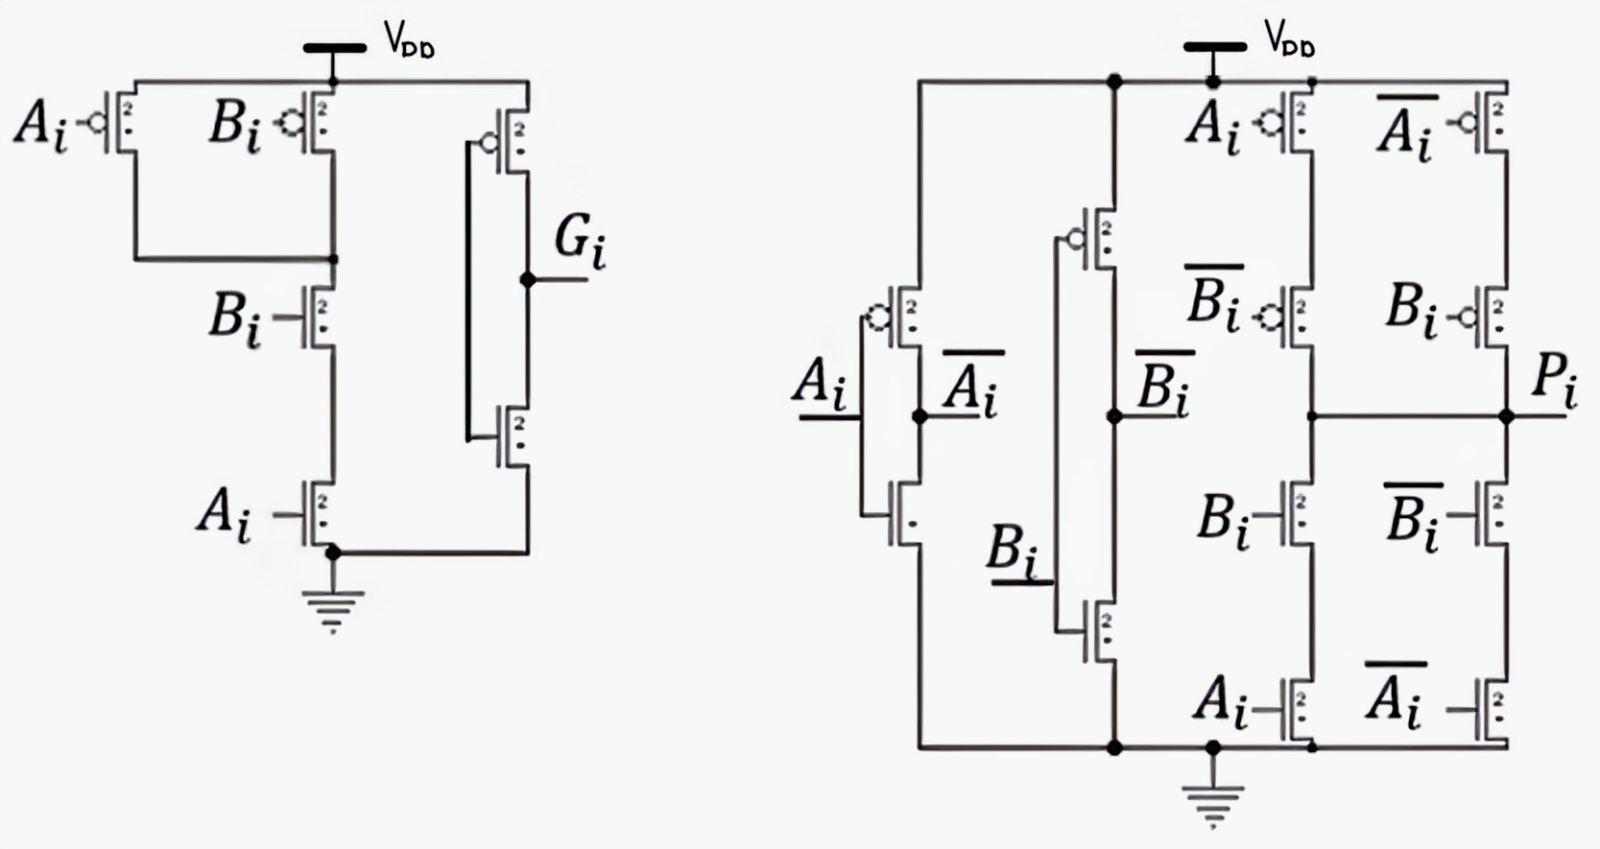
\includegraphics[width=1\linewidth]{gipi.jpg}
    \caption{$G_i$ (AND) and $P_i$ (XOR) gate.}
    \label{fig:enter-label}
\end{figure}
\begin{figure}[H]
    \centering
    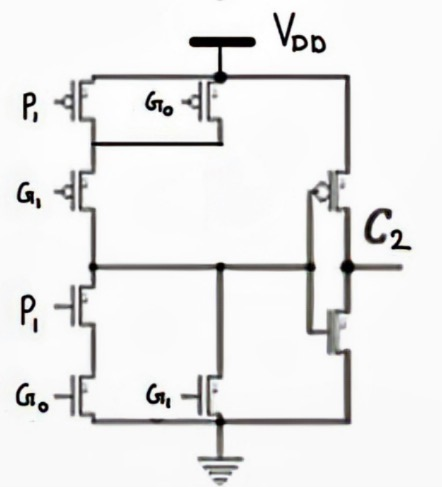
\includegraphics[width=0.5\linewidth]{c2.jpg}
    \caption{$C_2$}
    \label{fig:enter-label}
\end{figure}
\begin{figure}[H]
    \centering
    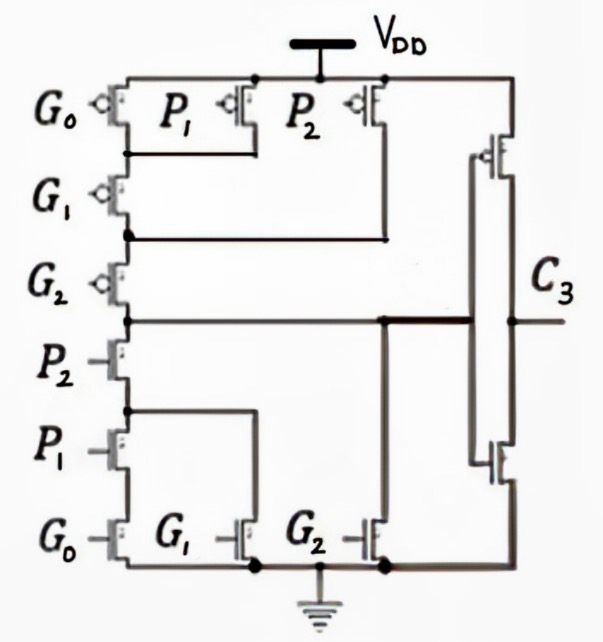
\includegraphics[width=0.5\linewidth]{c3.jpg}
    \caption{$C_3$}
    \label{fig:enter-label}
\end{figure}
\begin{figure}[H]
    \centering
    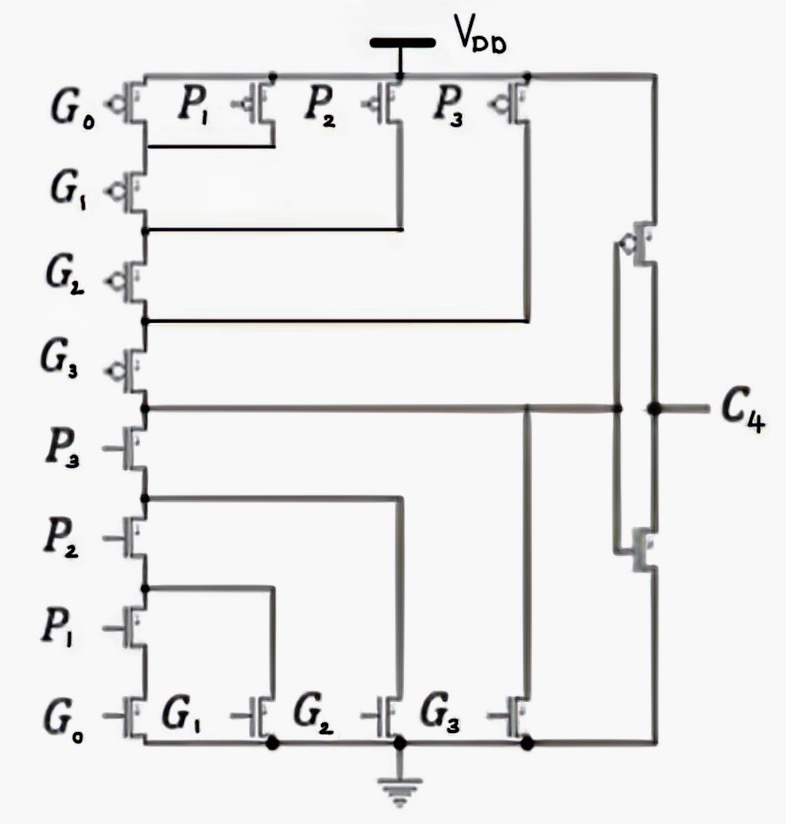
\includegraphics[width=0.5\linewidth]{c4.jpg}
    \caption{$C_4$}
    \label{fig:enter-label}
\end{figure}
Finally, we can realize the complete adder circuit.
\begin{figure}[H]
    \centering
    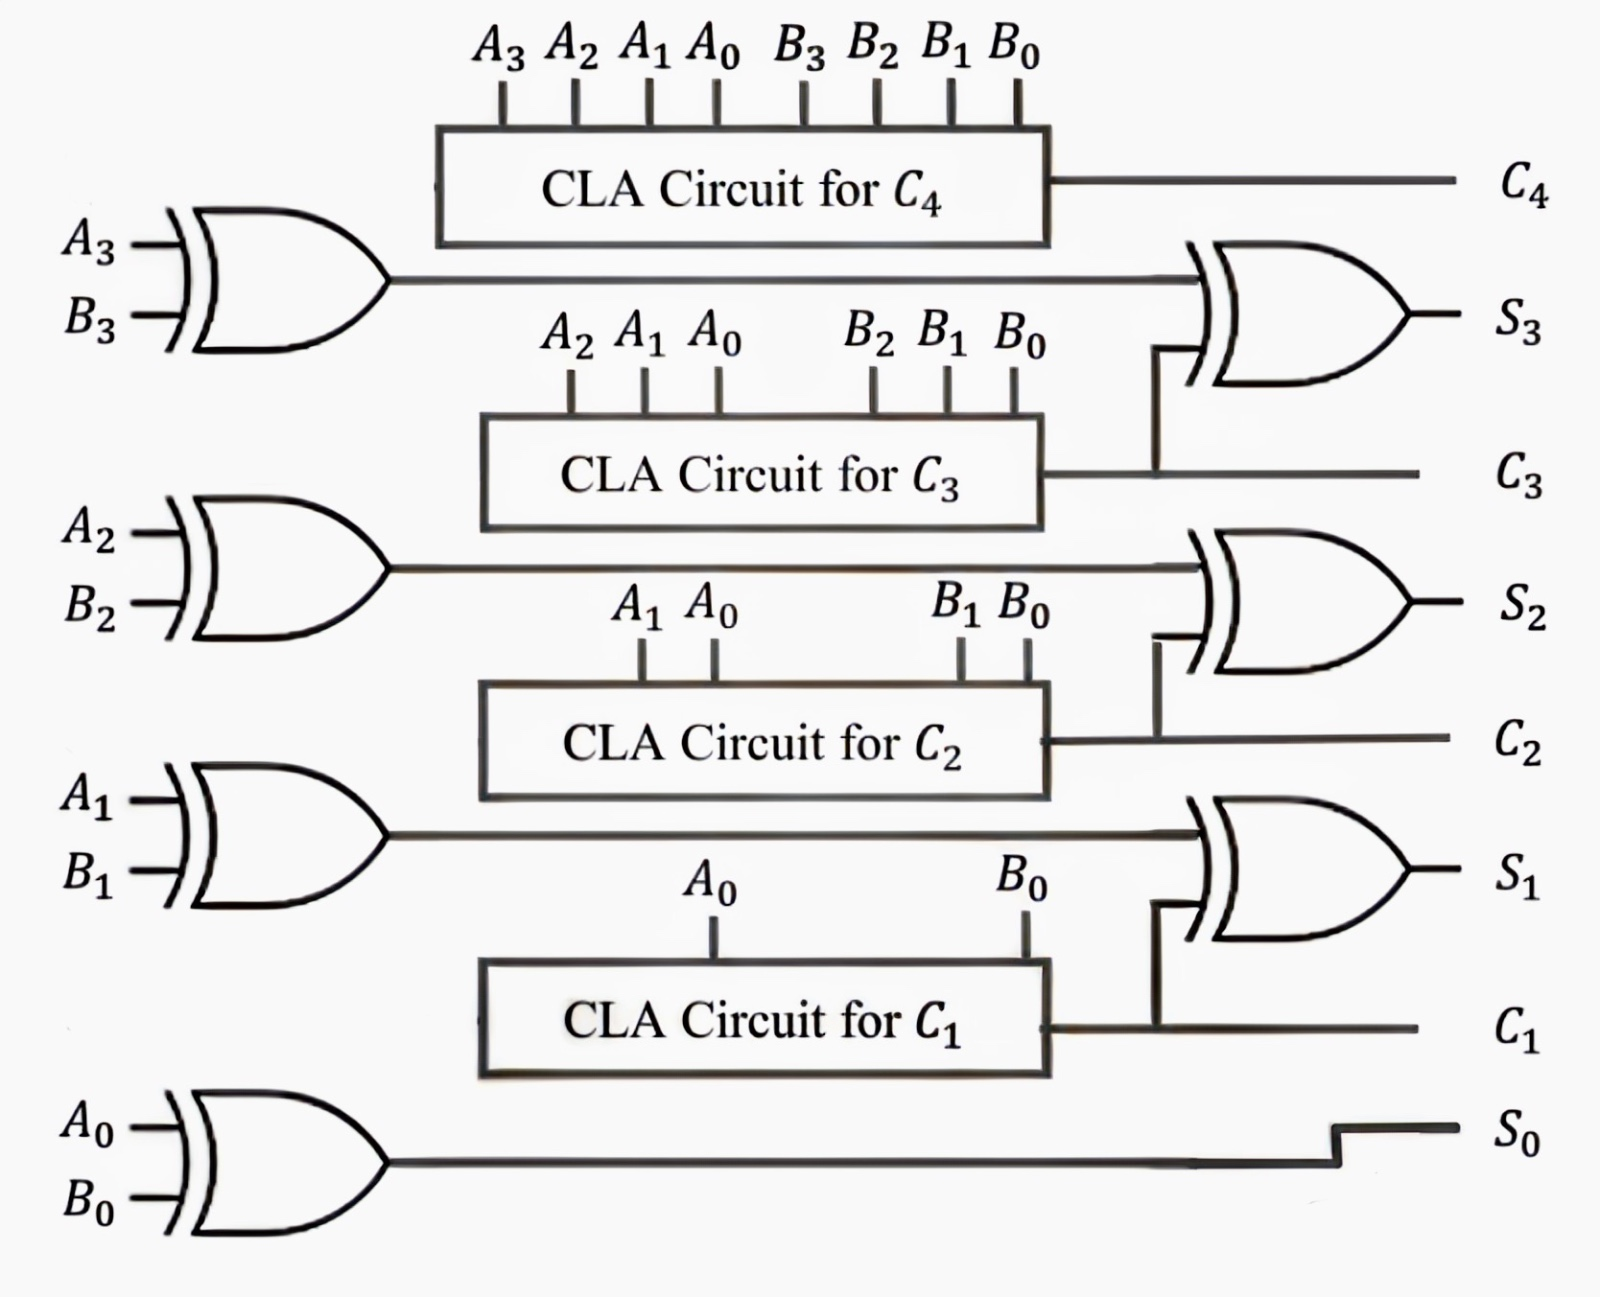
\includegraphics[width=1\linewidth]{cla.jpg}
    \caption{Logic gate level representation of static based CMOS CLA adder}
    \label{fig:enter-label}
\end{figure}
where each carry compute block combines $G_i$ and $P_i$ calculate blocks and carry compute logic circuits as realized before.\newline
The combinational logic is synchronized with clock signal using sequential TSPC logic based D-Flip-Flop. The circuit is shown below. 
\begin{figure}[H]
    \centering
    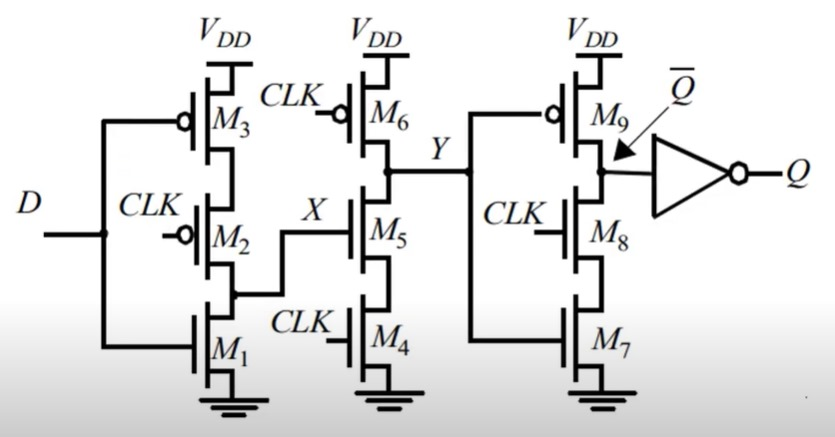
\includegraphics[width=1\linewidth]{dff.jpg}
    \caption{D Flip Flop}
    \label{fig:enter-label}
\end{figure}

\section{CMOS sizing and Layout Design Strategy}
A modified euler path based approach was used to design layout in later section. Therefore a conservative approach was used to size mosfet's with respect to the propagation delay's they provided. Most modules shown before performed best with a constant size ratio of 2W/W. But, it was noticed theoretical size of 2W/2W for AND gate performed best and so 2W/2W was used AND gate only. Also it, was noticed XOR gate performed the best for a 4W/W ratio but the delay improvement was very less so the constant size of 2W/W was chosen to construct a symmetric layout. A symmetric equi-sized static logic was designed to construct a euler path based layout.\newline
An Euler path, in a circuit, is a walk through the graph which uses every edge exactly once. An Euler circuit is an Euler path which starts and stops at the same vertex. Euler path's were constructed for all modules but in this process only one mosfet from PDN/PUN was connected to $V_{DD}$ or Gnd. This resulted in higher rise/fall time which are critical to minimizing delay. Therefore the logic was seperated into smaller parts and the layout was constructed. This is discussed in later stages. \newline
D Flip Flop showed no improvement on increasing size or ratio. Therefore, a small size of 2W/W was chosen for TSPC DFF to add a lesser load on clock signal. 

\section{Simulation of different modules using NGSPICE}
The loaded simulations were performed to determine the functionality of circuit by writing a ngspice netlist. 
\begin{figure}[H]
    \centering
    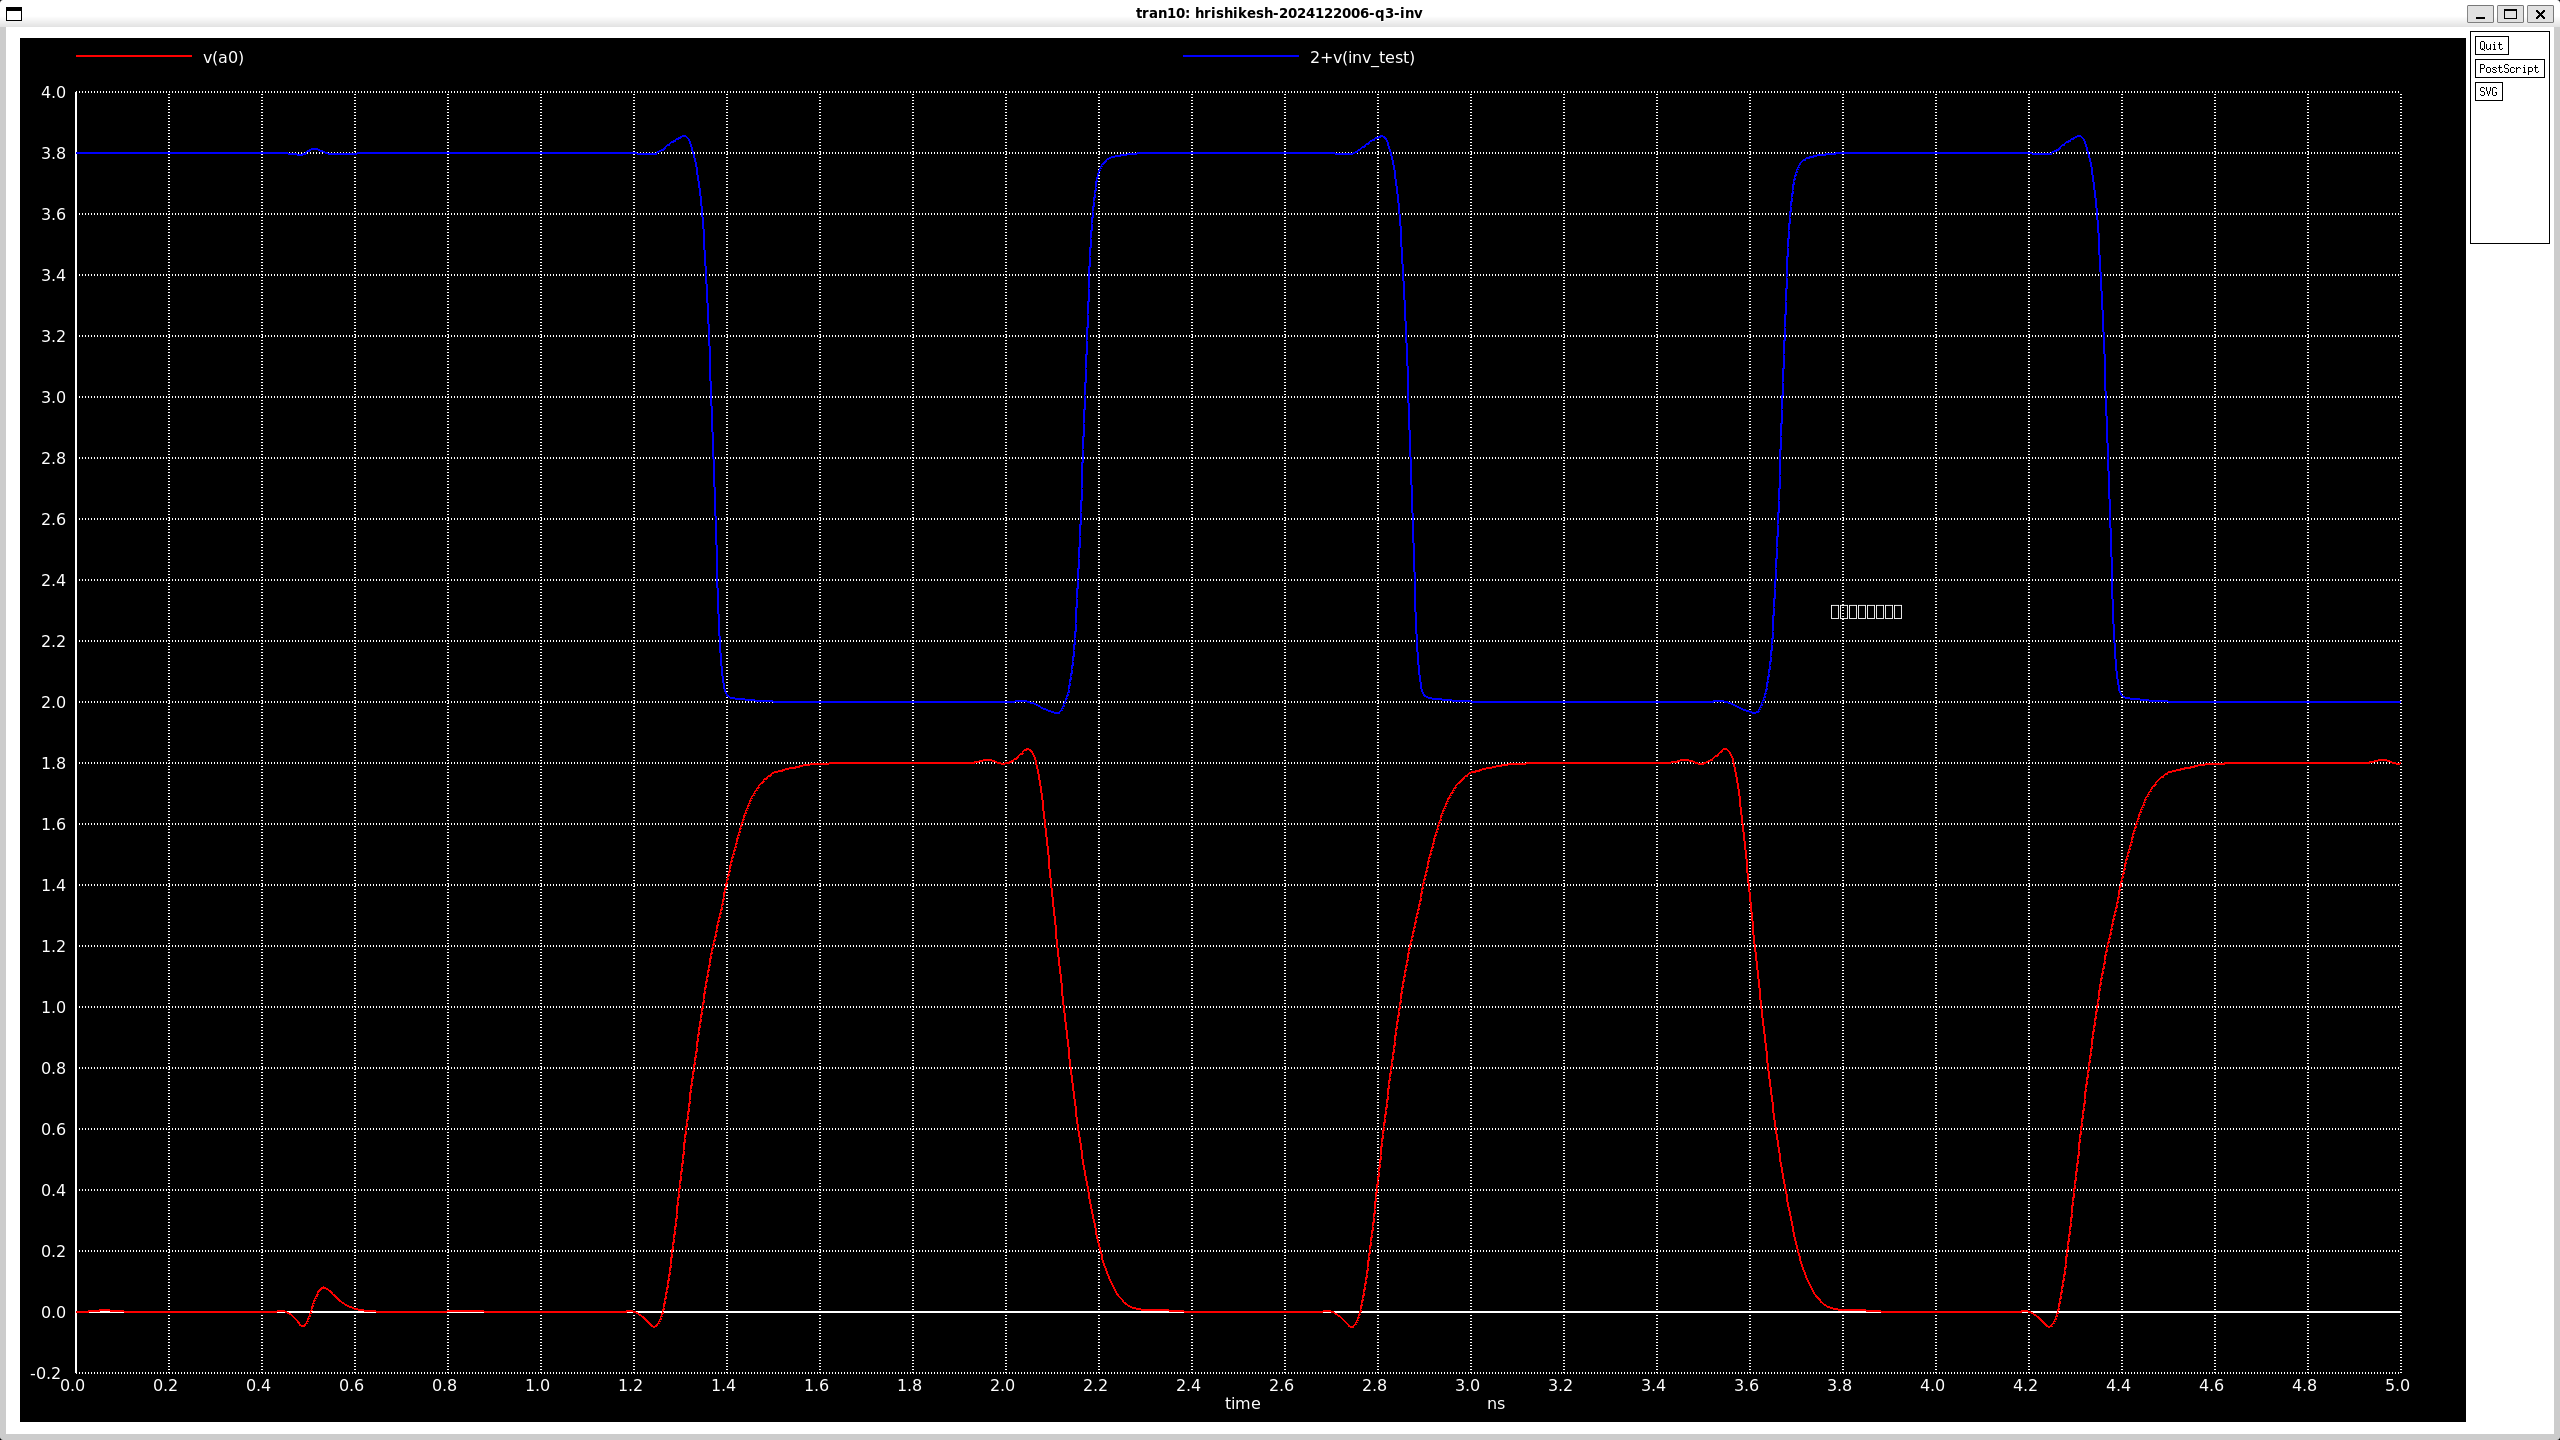
\includegraphics[width=1\linewidth]{inverter_module.png}
    \caption{CMOS Inverter}
    \label{fig:enter-label}
\end{figure}
\begin{figure}[H]
    \centering
    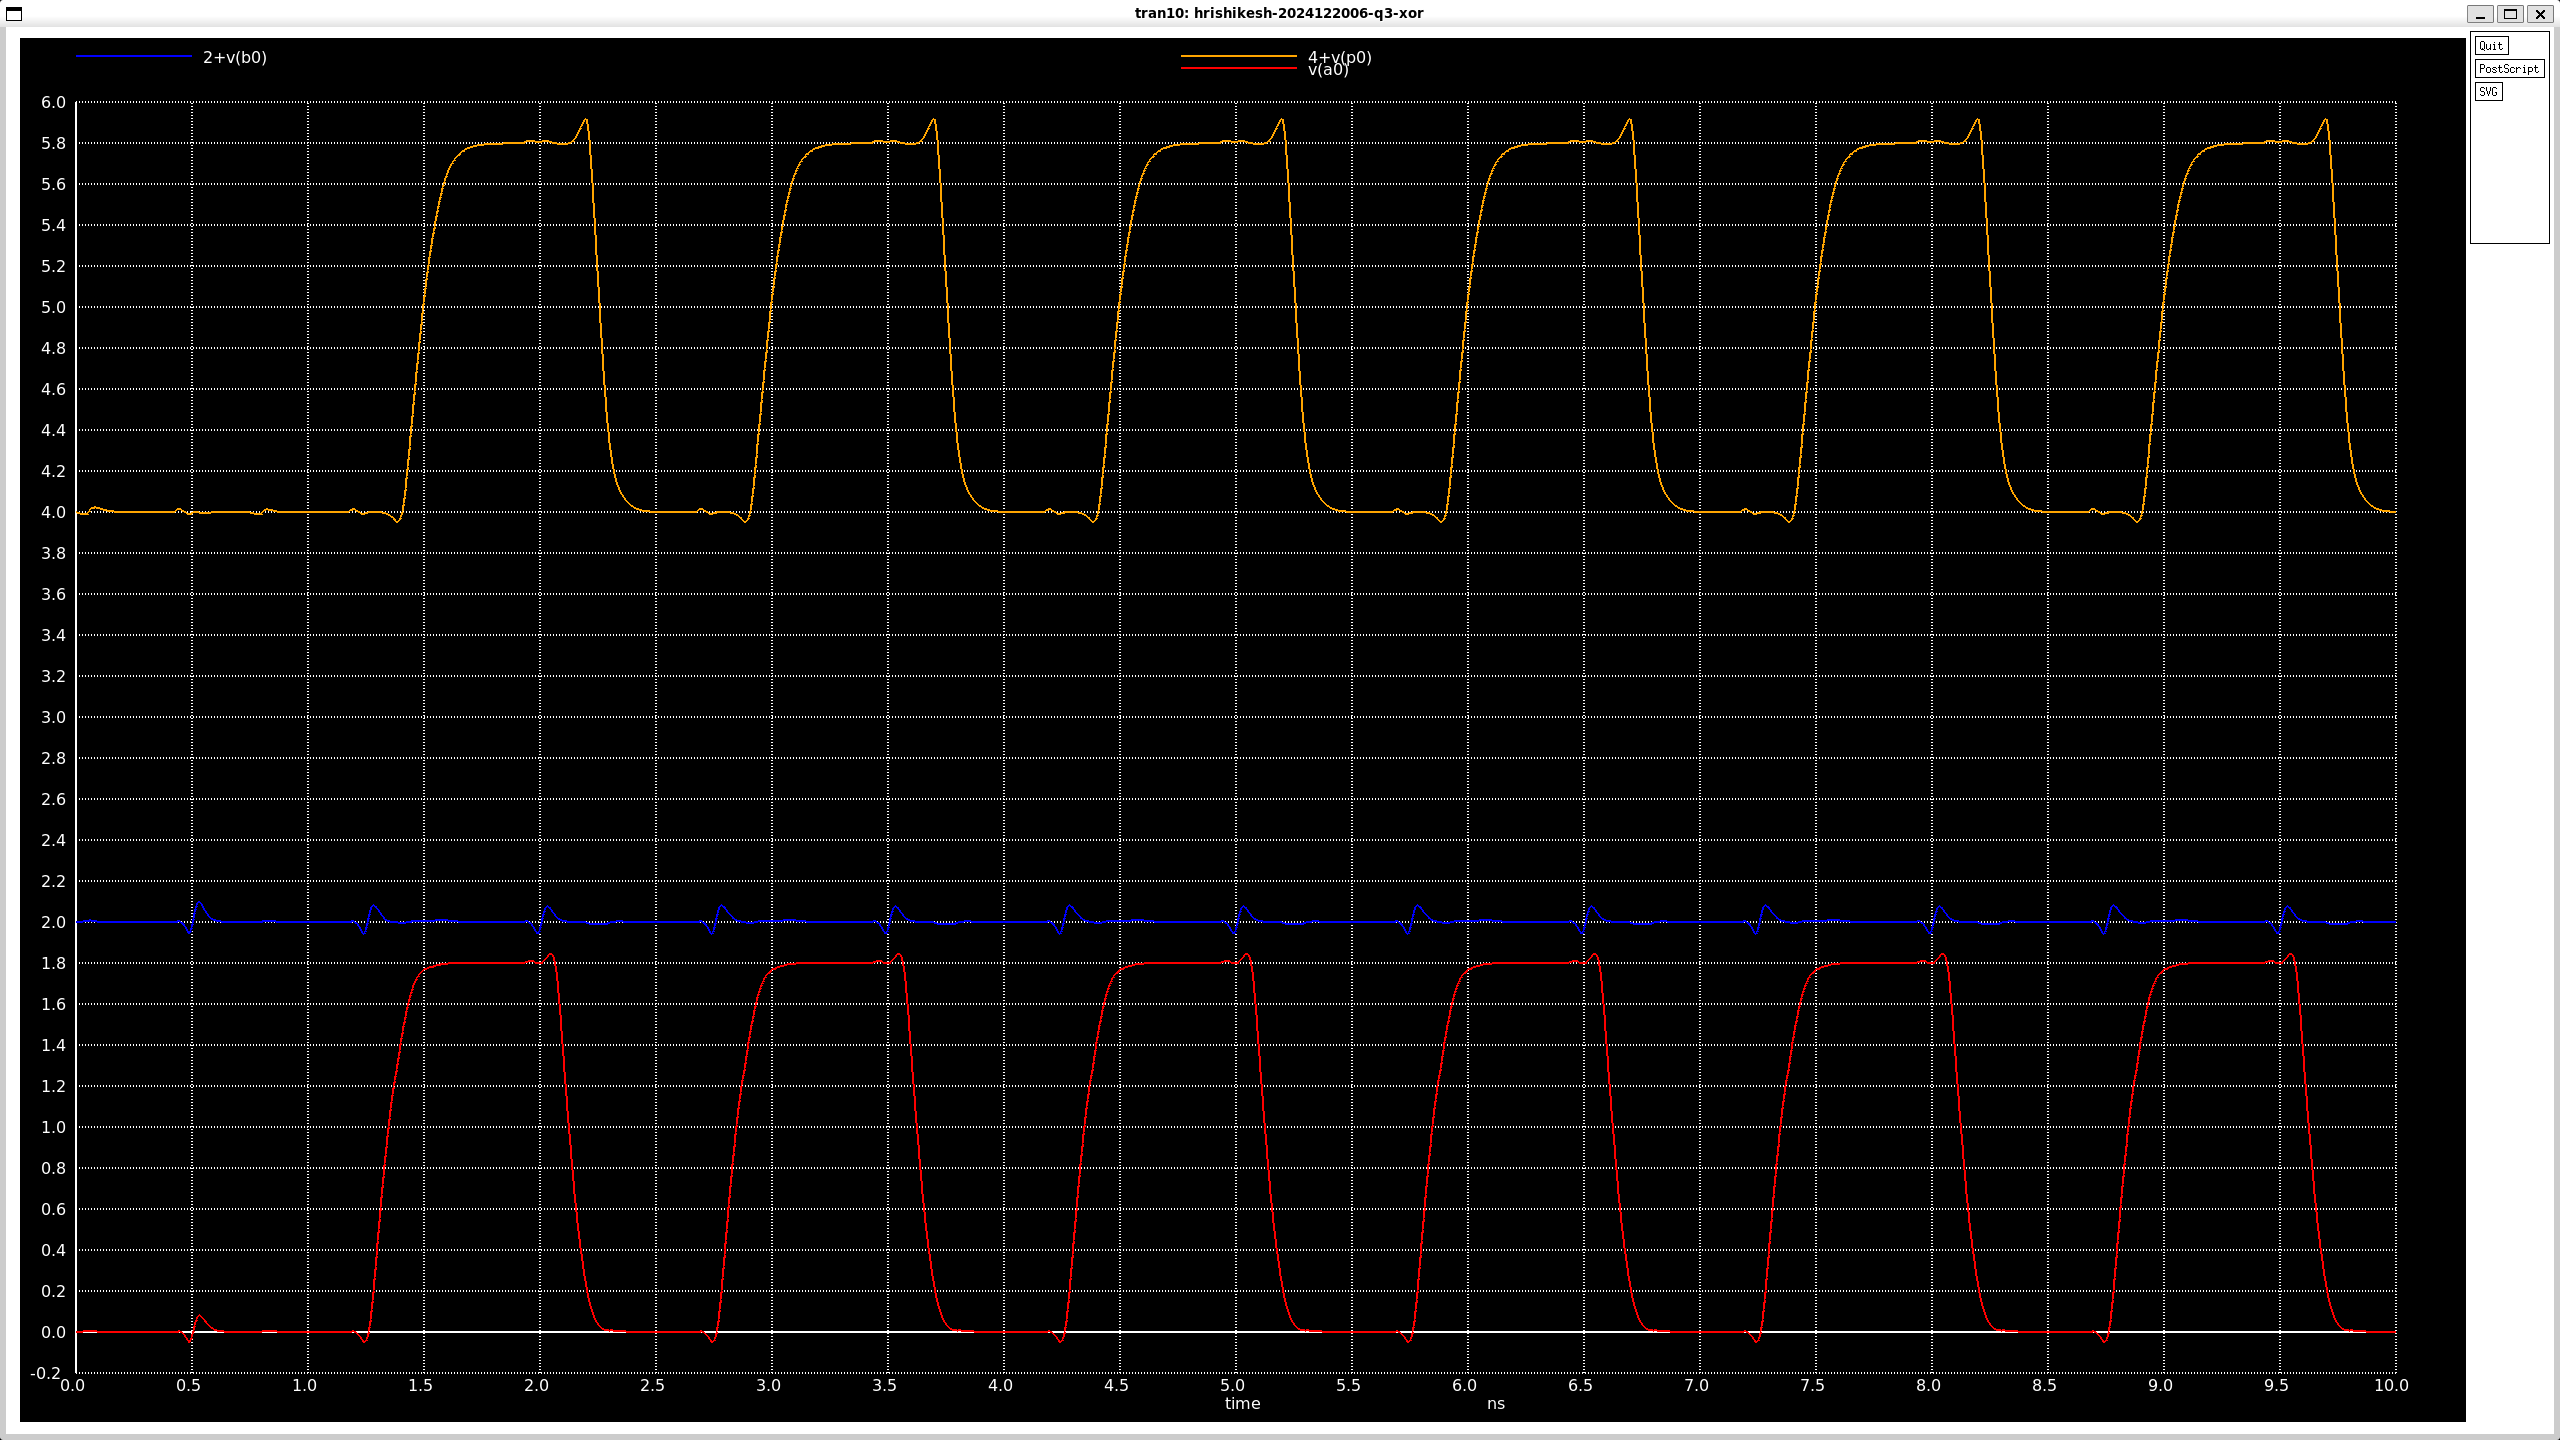
\includegraphics[width=1\linewidth]{xor_module.png}
    \caption{XOR Gate}
    \label{fig:enter-label}
\end{figure}
\begin{figure}[H]
    \centering
    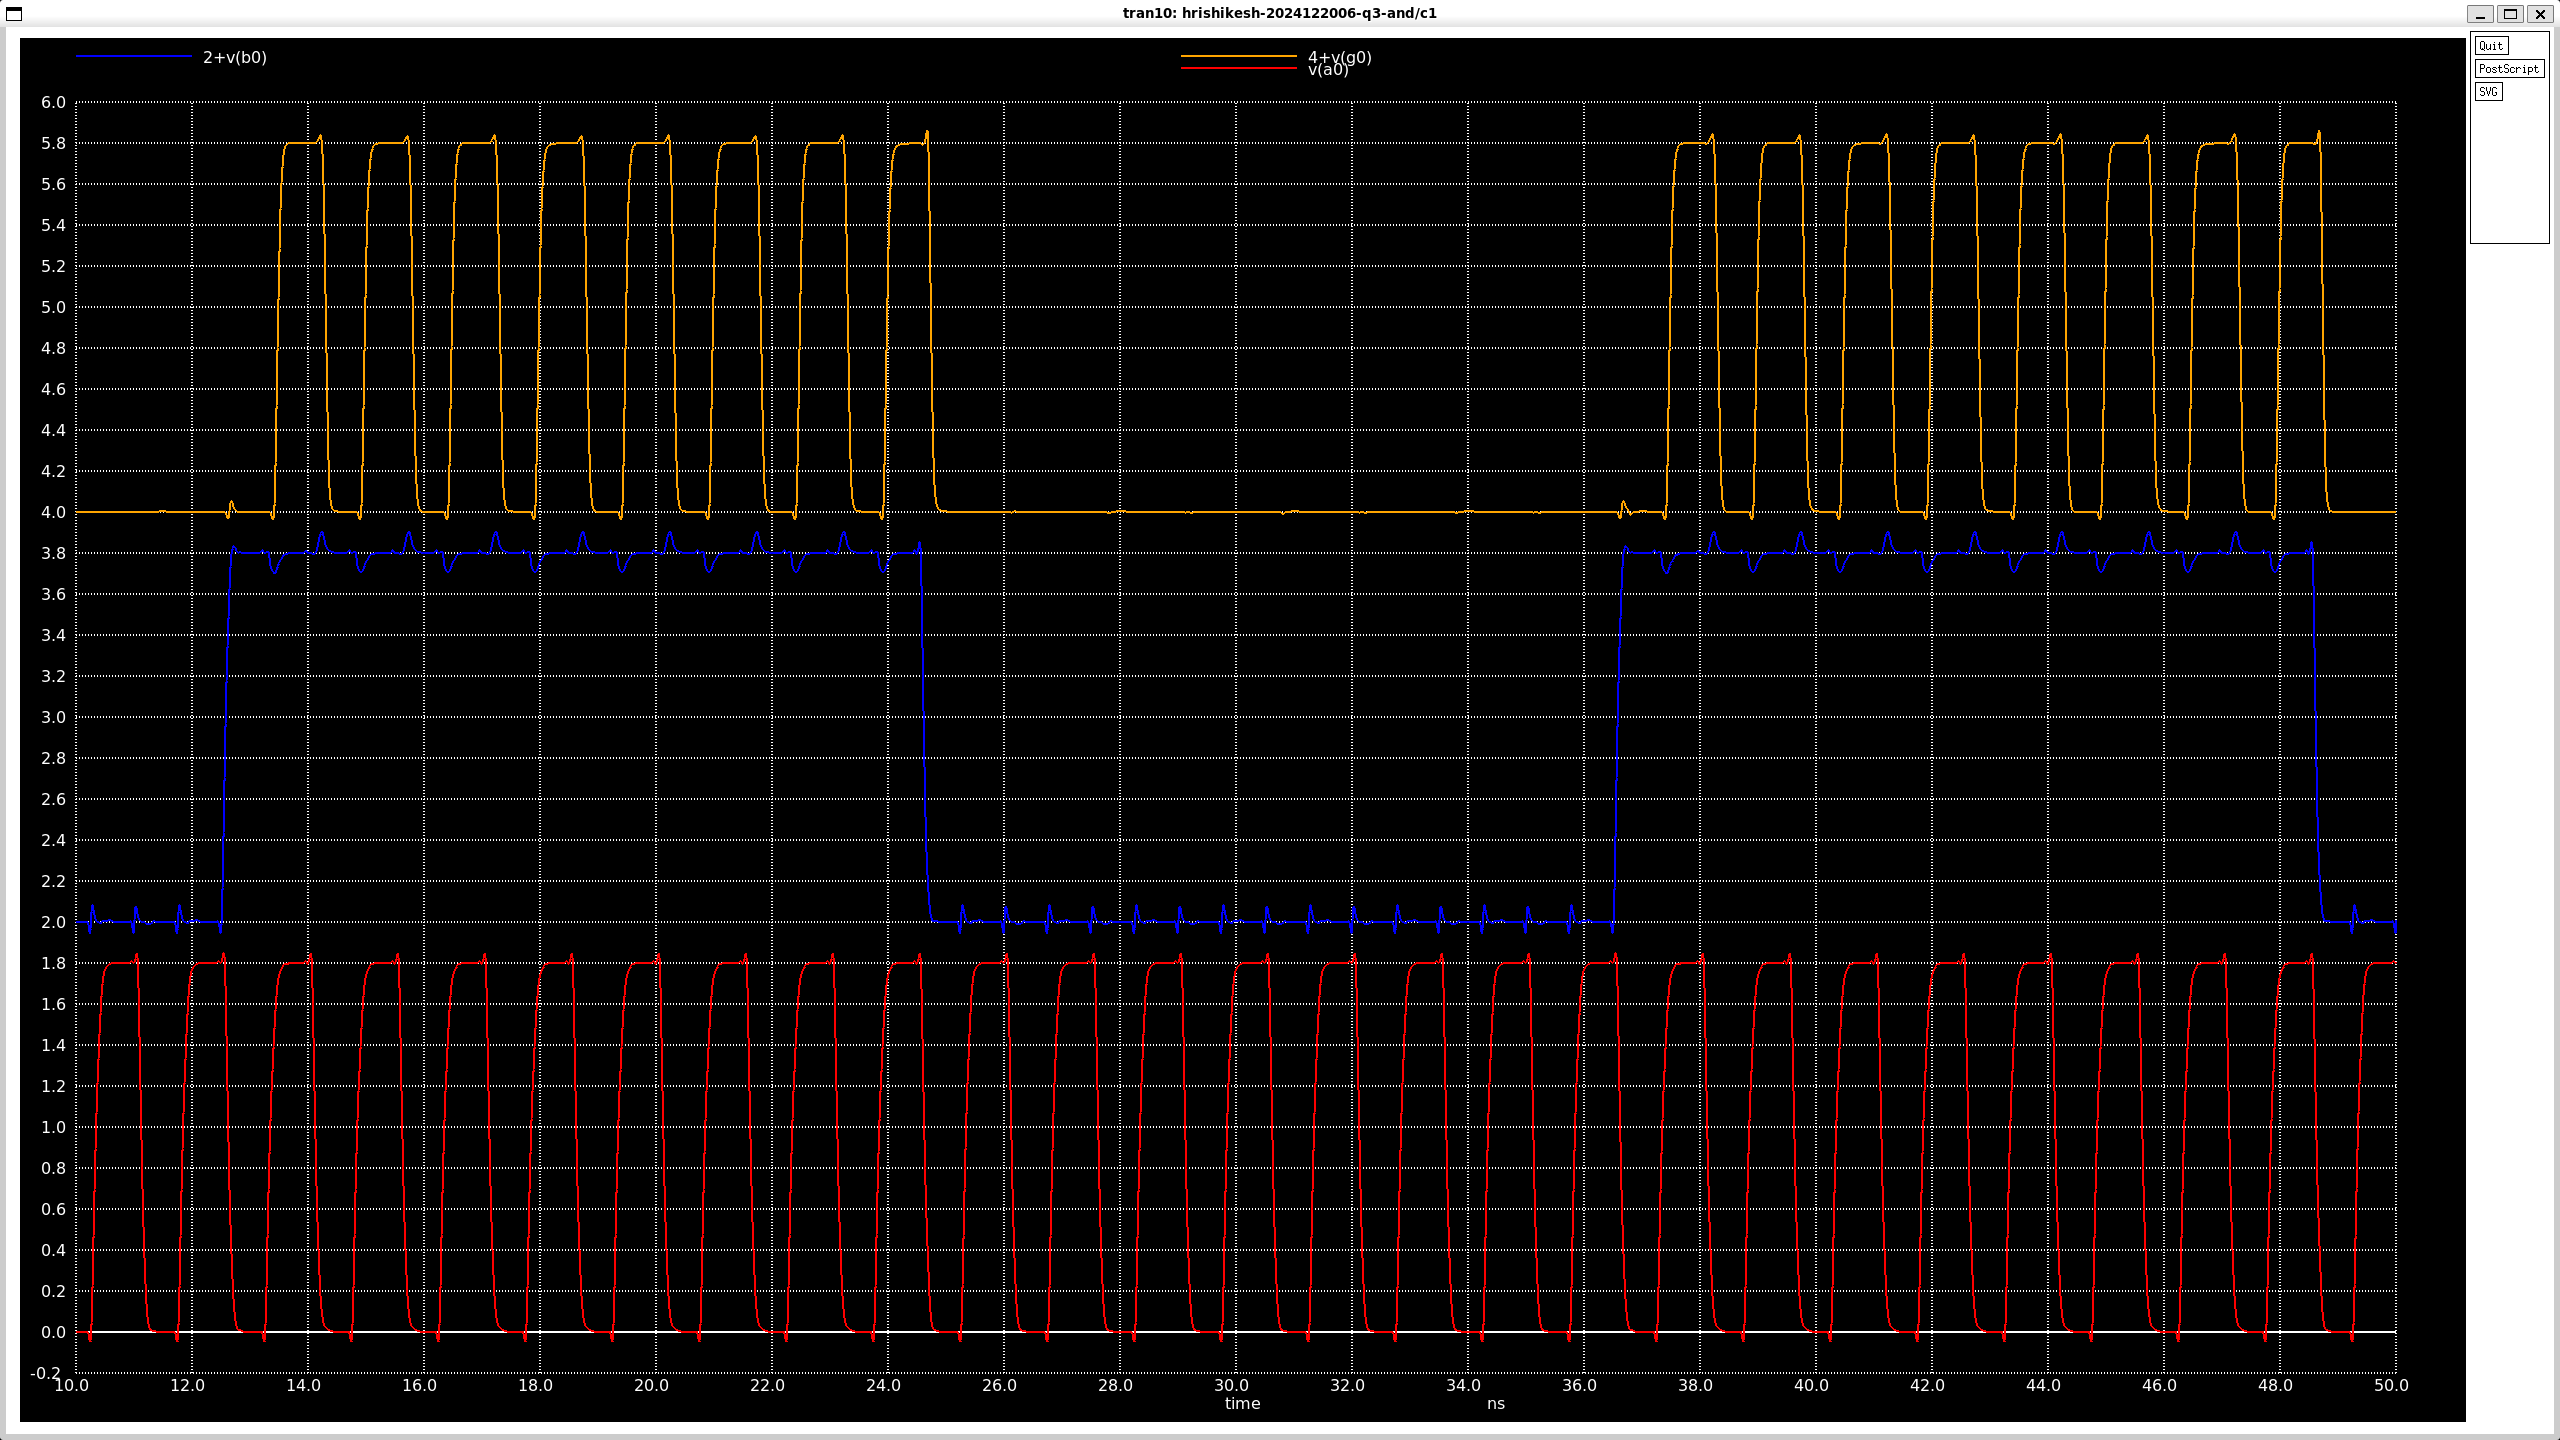
\includegraphics[width=1\linewidth]{and_module.png}
    \caption{AND Gate}
    \label{fig:enter-label}
\end{figure}
\begin{figure}[H]
    \centering
    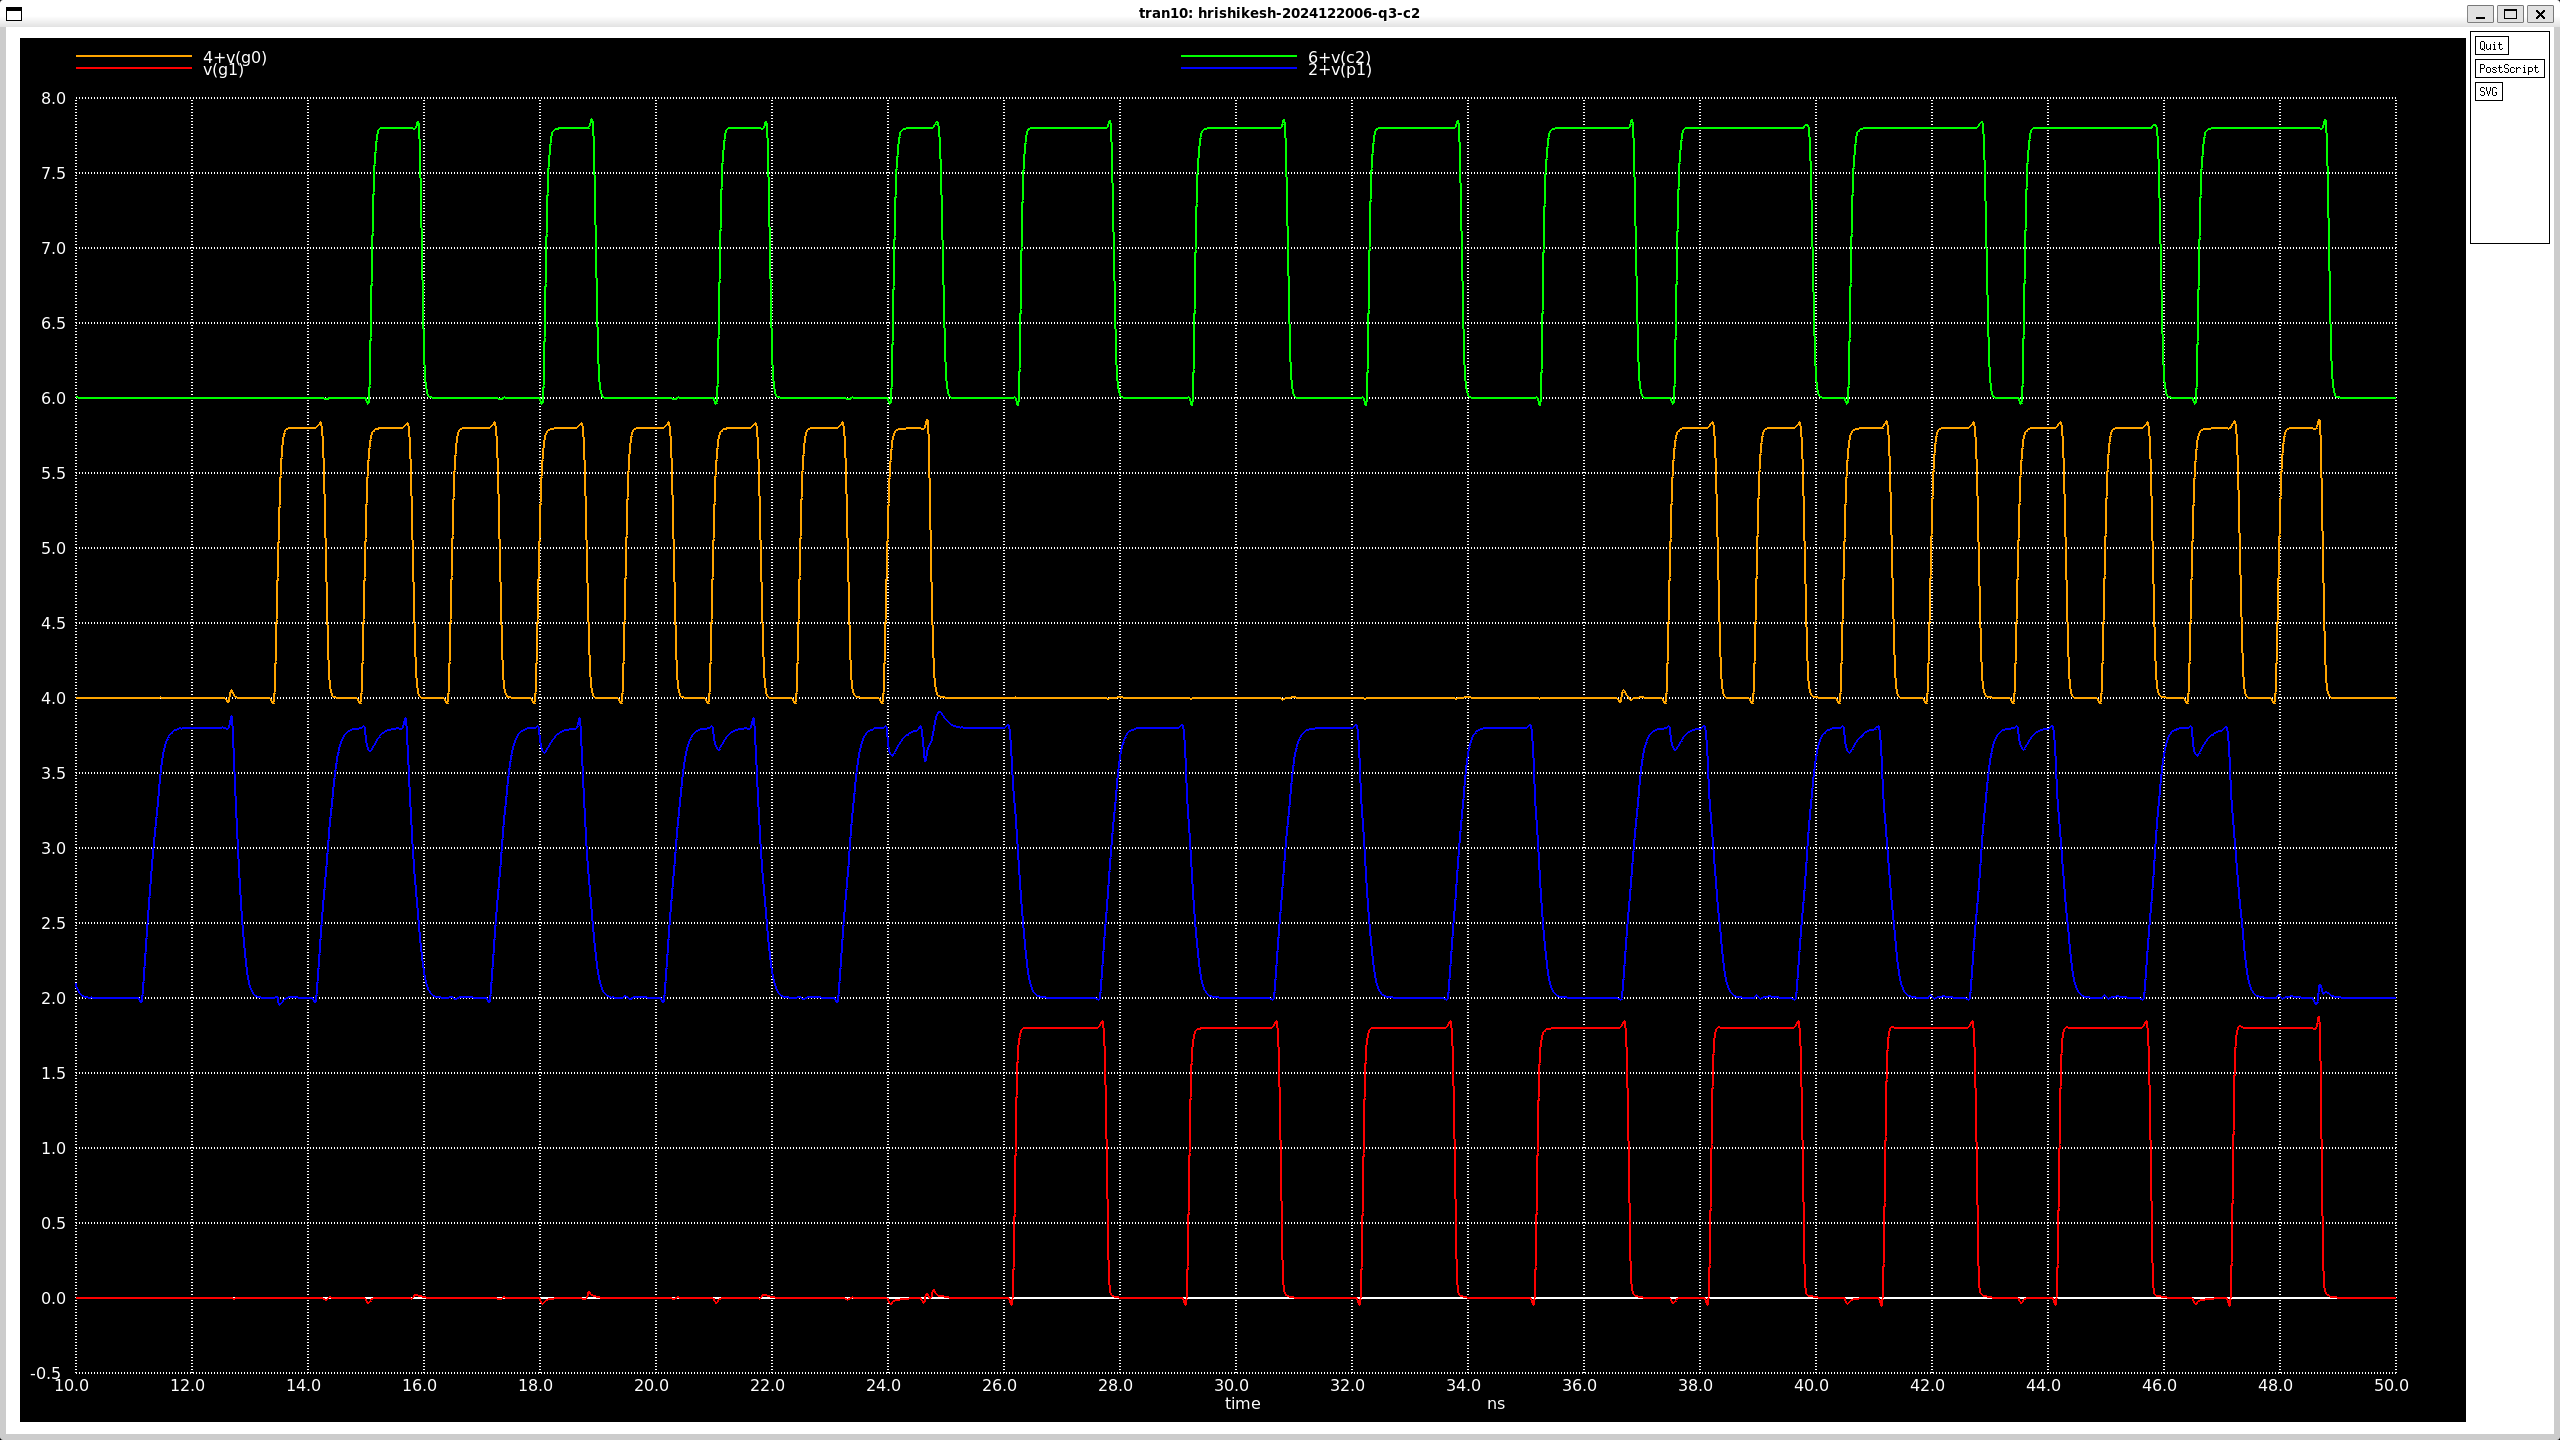
\includegraphics[width=1\linewidth]{c2_module.png}
    \caption{$C_2$ Logic}
    \label{fig:enter-label}
\end{figure}
\begin{figure}[H]
    \centering
    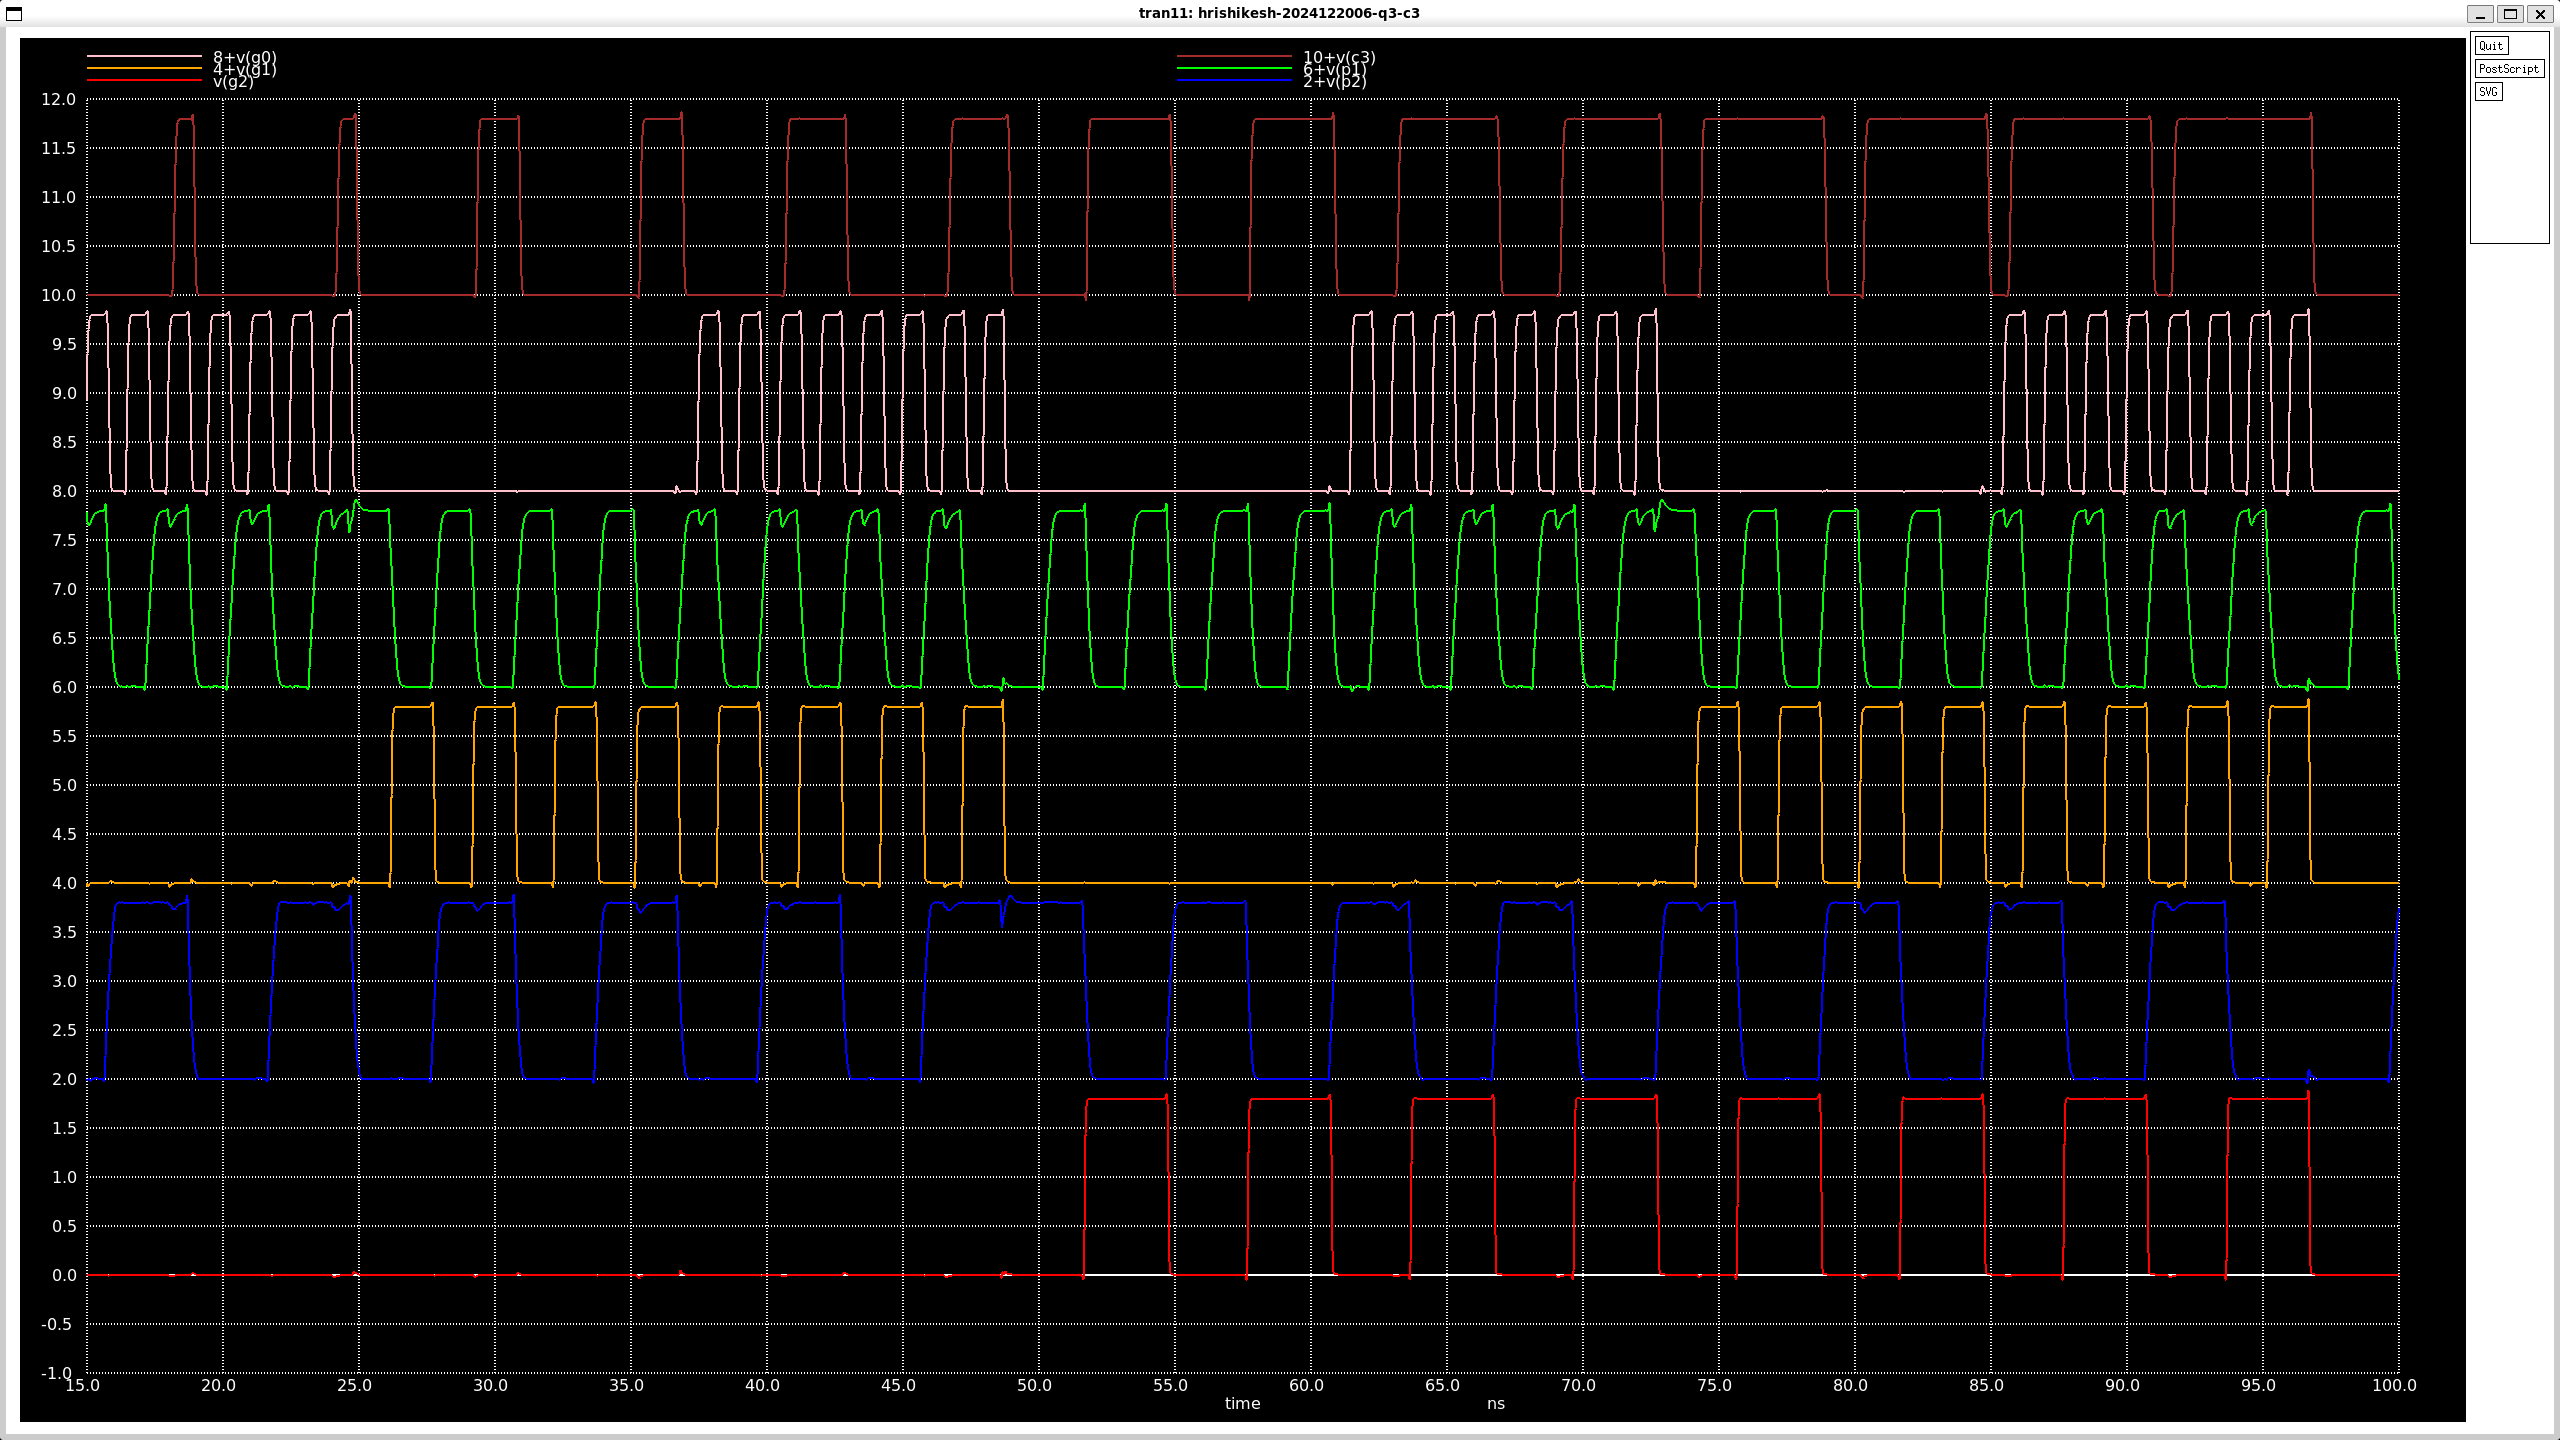
\includegraphics[width=1\linewidth]{c3_module.png}
    \caption{$C_3$ Logic}
    \label{fig:enter-label}
\end{figure}
\begin{figure}[H]
    \centering
    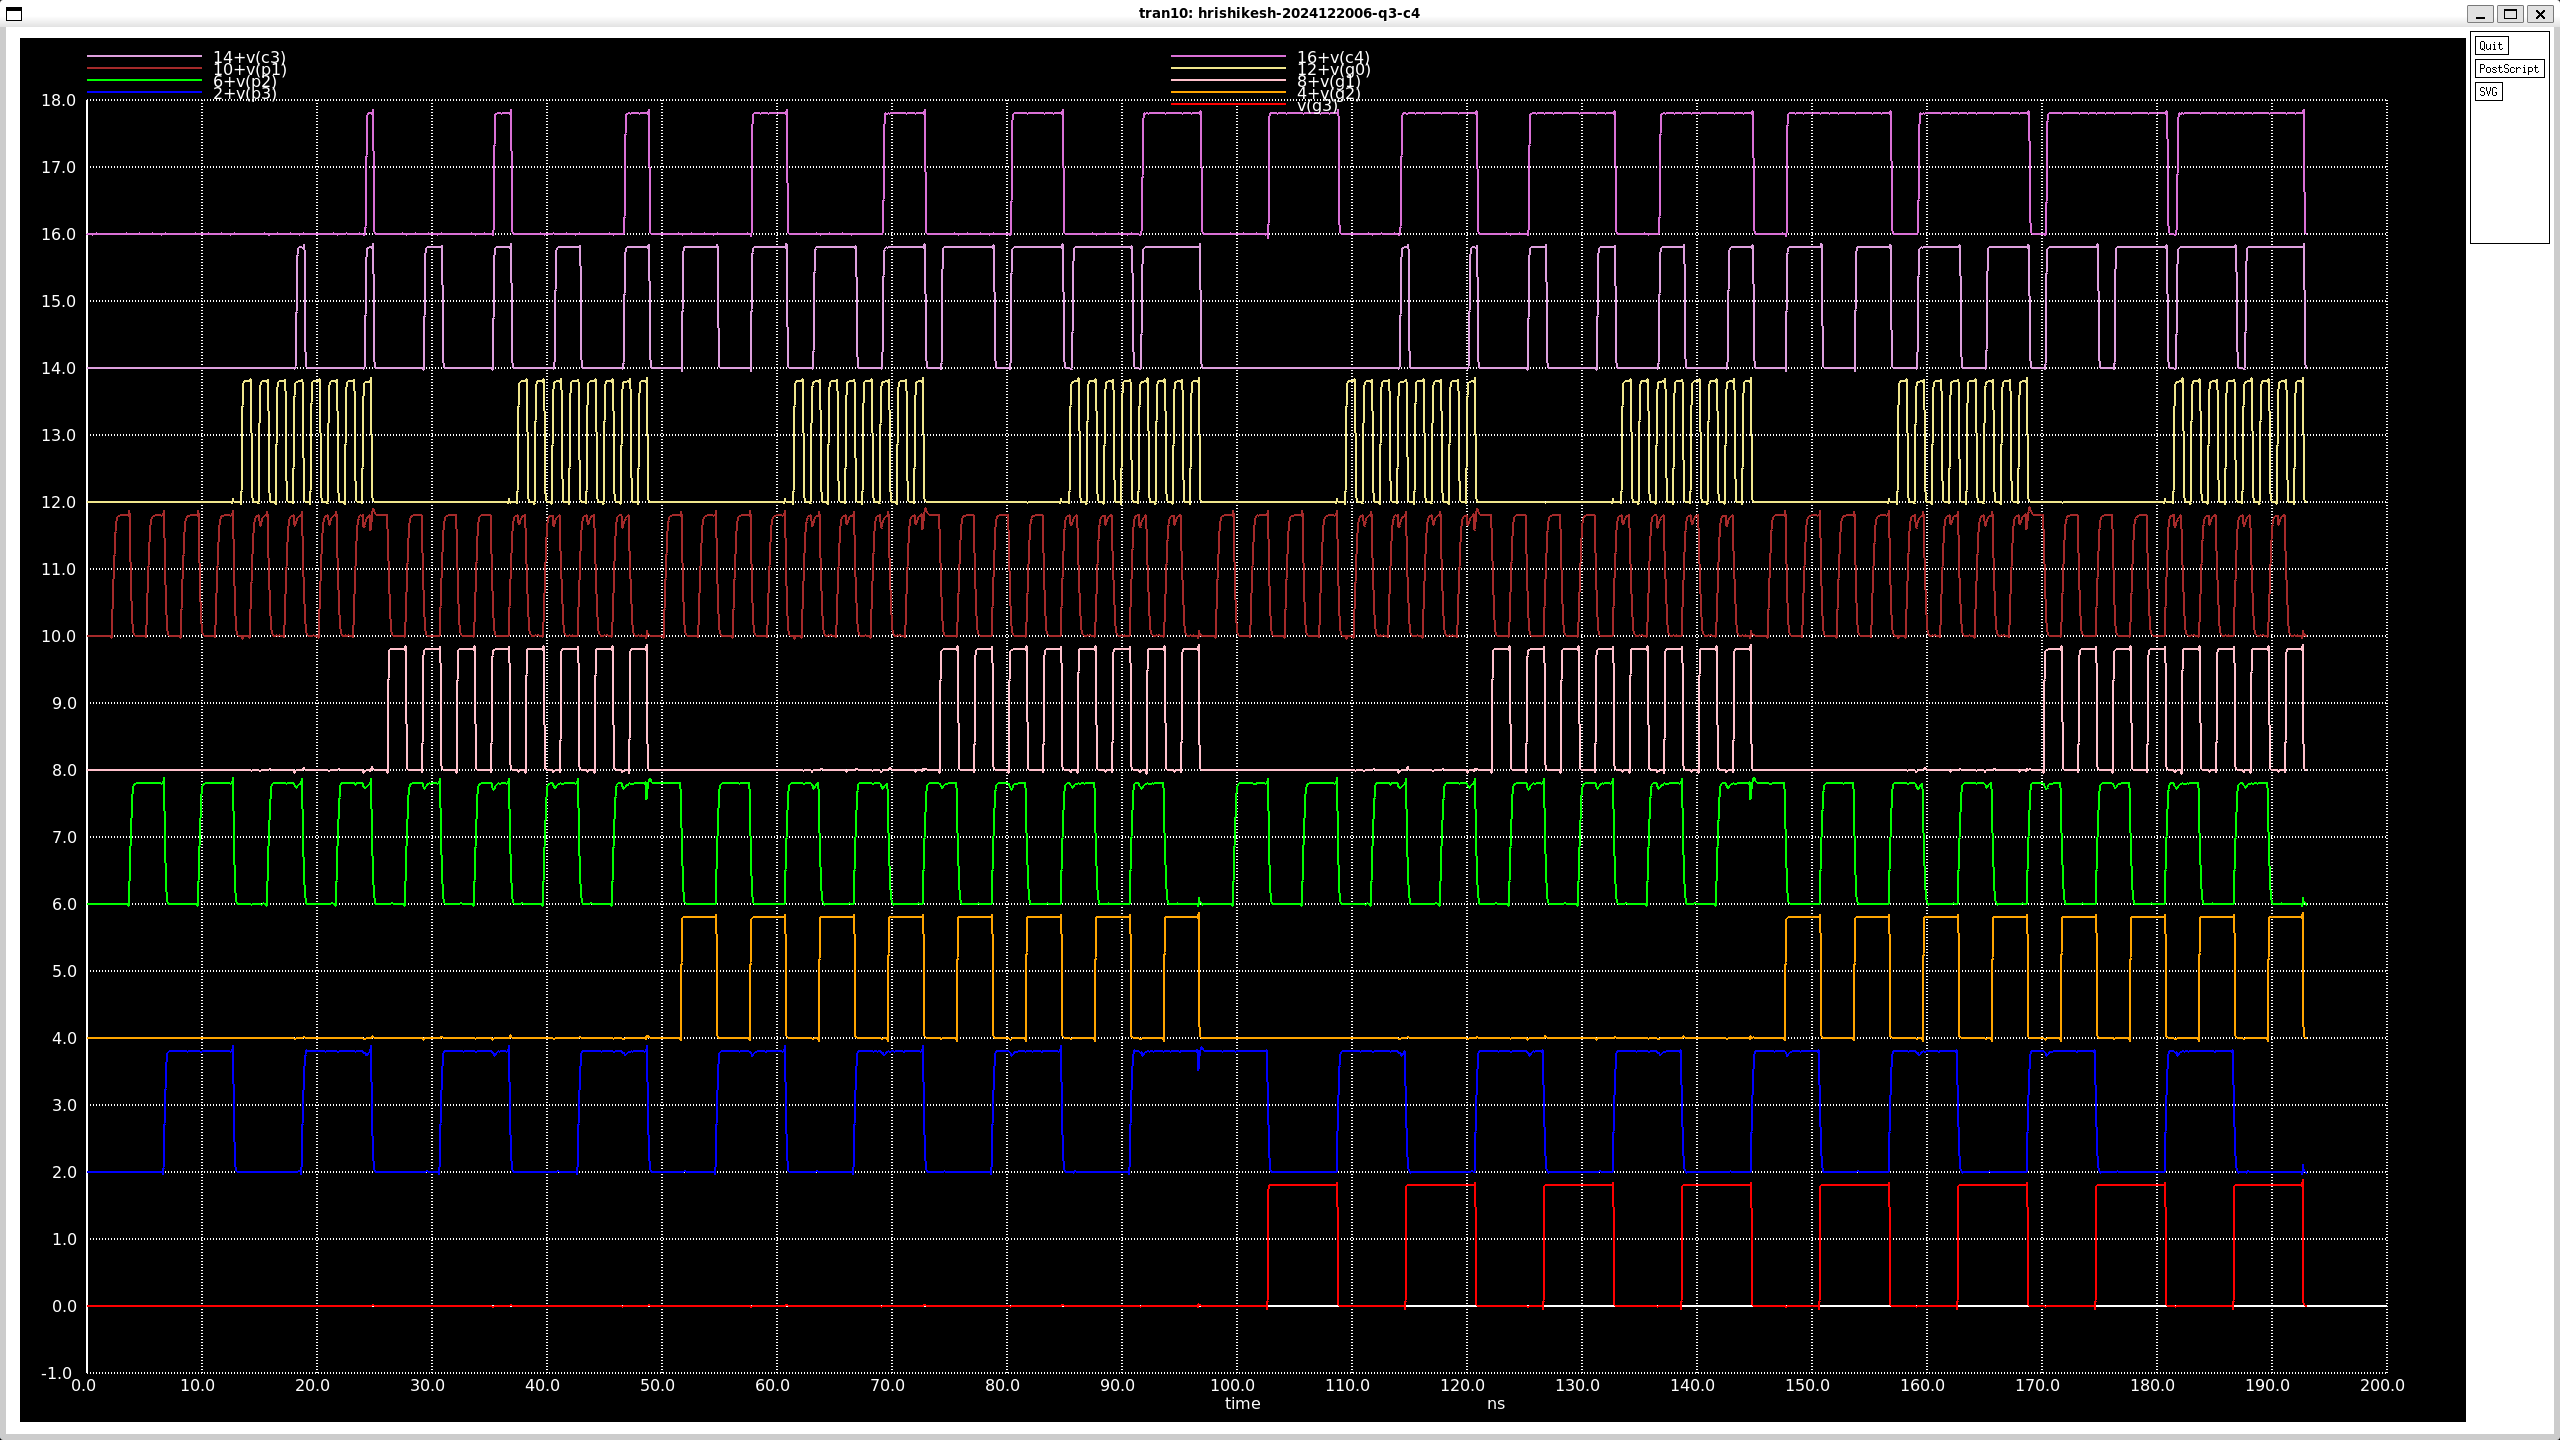
\includegraphics[width=1\linewidth]{c4_module.png}
    \caption{$C_4$ Logic}
    \label{fig:enter-label}
\end{figure}
The modules' propagation delay and power consumed are tabulated below.
\begin{center}
\begin{tabular}{ | m{2cm} | m{2cm}| m{2.5cm} | } 
  \hline
  Module & Delay (s) & RMS Power (W) \\ 
  \hline
  Inverter & 5.30549e-11 & 2.08383e-04 \\ 
  \hline
  XOR Gate & 1.38618e-10 & 3.34009e-04 \\ 
  \hline
  AND Gate & 1.59971e-10 & 4.97616e-04 \\ 
  \hline
  $C_2$ Logic & 2.86838e-10 & 2.43924e-04 \\ 
  \hline
  $C_3$ Logic & 3.89675e-10 & 1.90786e-04 \\ 
  \hline
  $C_4$ Logic & 4.97499e-10 & 1.47645e-04 \\ 
  \hline
\end{tabular}
\end{center}

\section{D Flip-Flop}
A positive edge-triggered D flip-flop based on TSPC logic is used to synchronize CLA i/o's with clock and for data storage which provides better timing control. The schematic for this flip flop is provided in section I.
\[
\begin{array}{|c|c|c|}
\hline
\textbf{Clock} (\uparrow) & \textbf{D} (\text{Input}) & \textbf{Q} (\text{NextState}) \\ \hline
\uparrow & 0 & 0 \\ \hline
\uparrow & 1 & 1 \\ \hline
X & X & Q \\ \hline
\end{array}
\]
To find the propagation delay from CLK edge to Q, a clock signal with 50 ps rise and fall time was used and a sufficiently long time period was chosen. 
\begin{figure}[H]
    \centering
    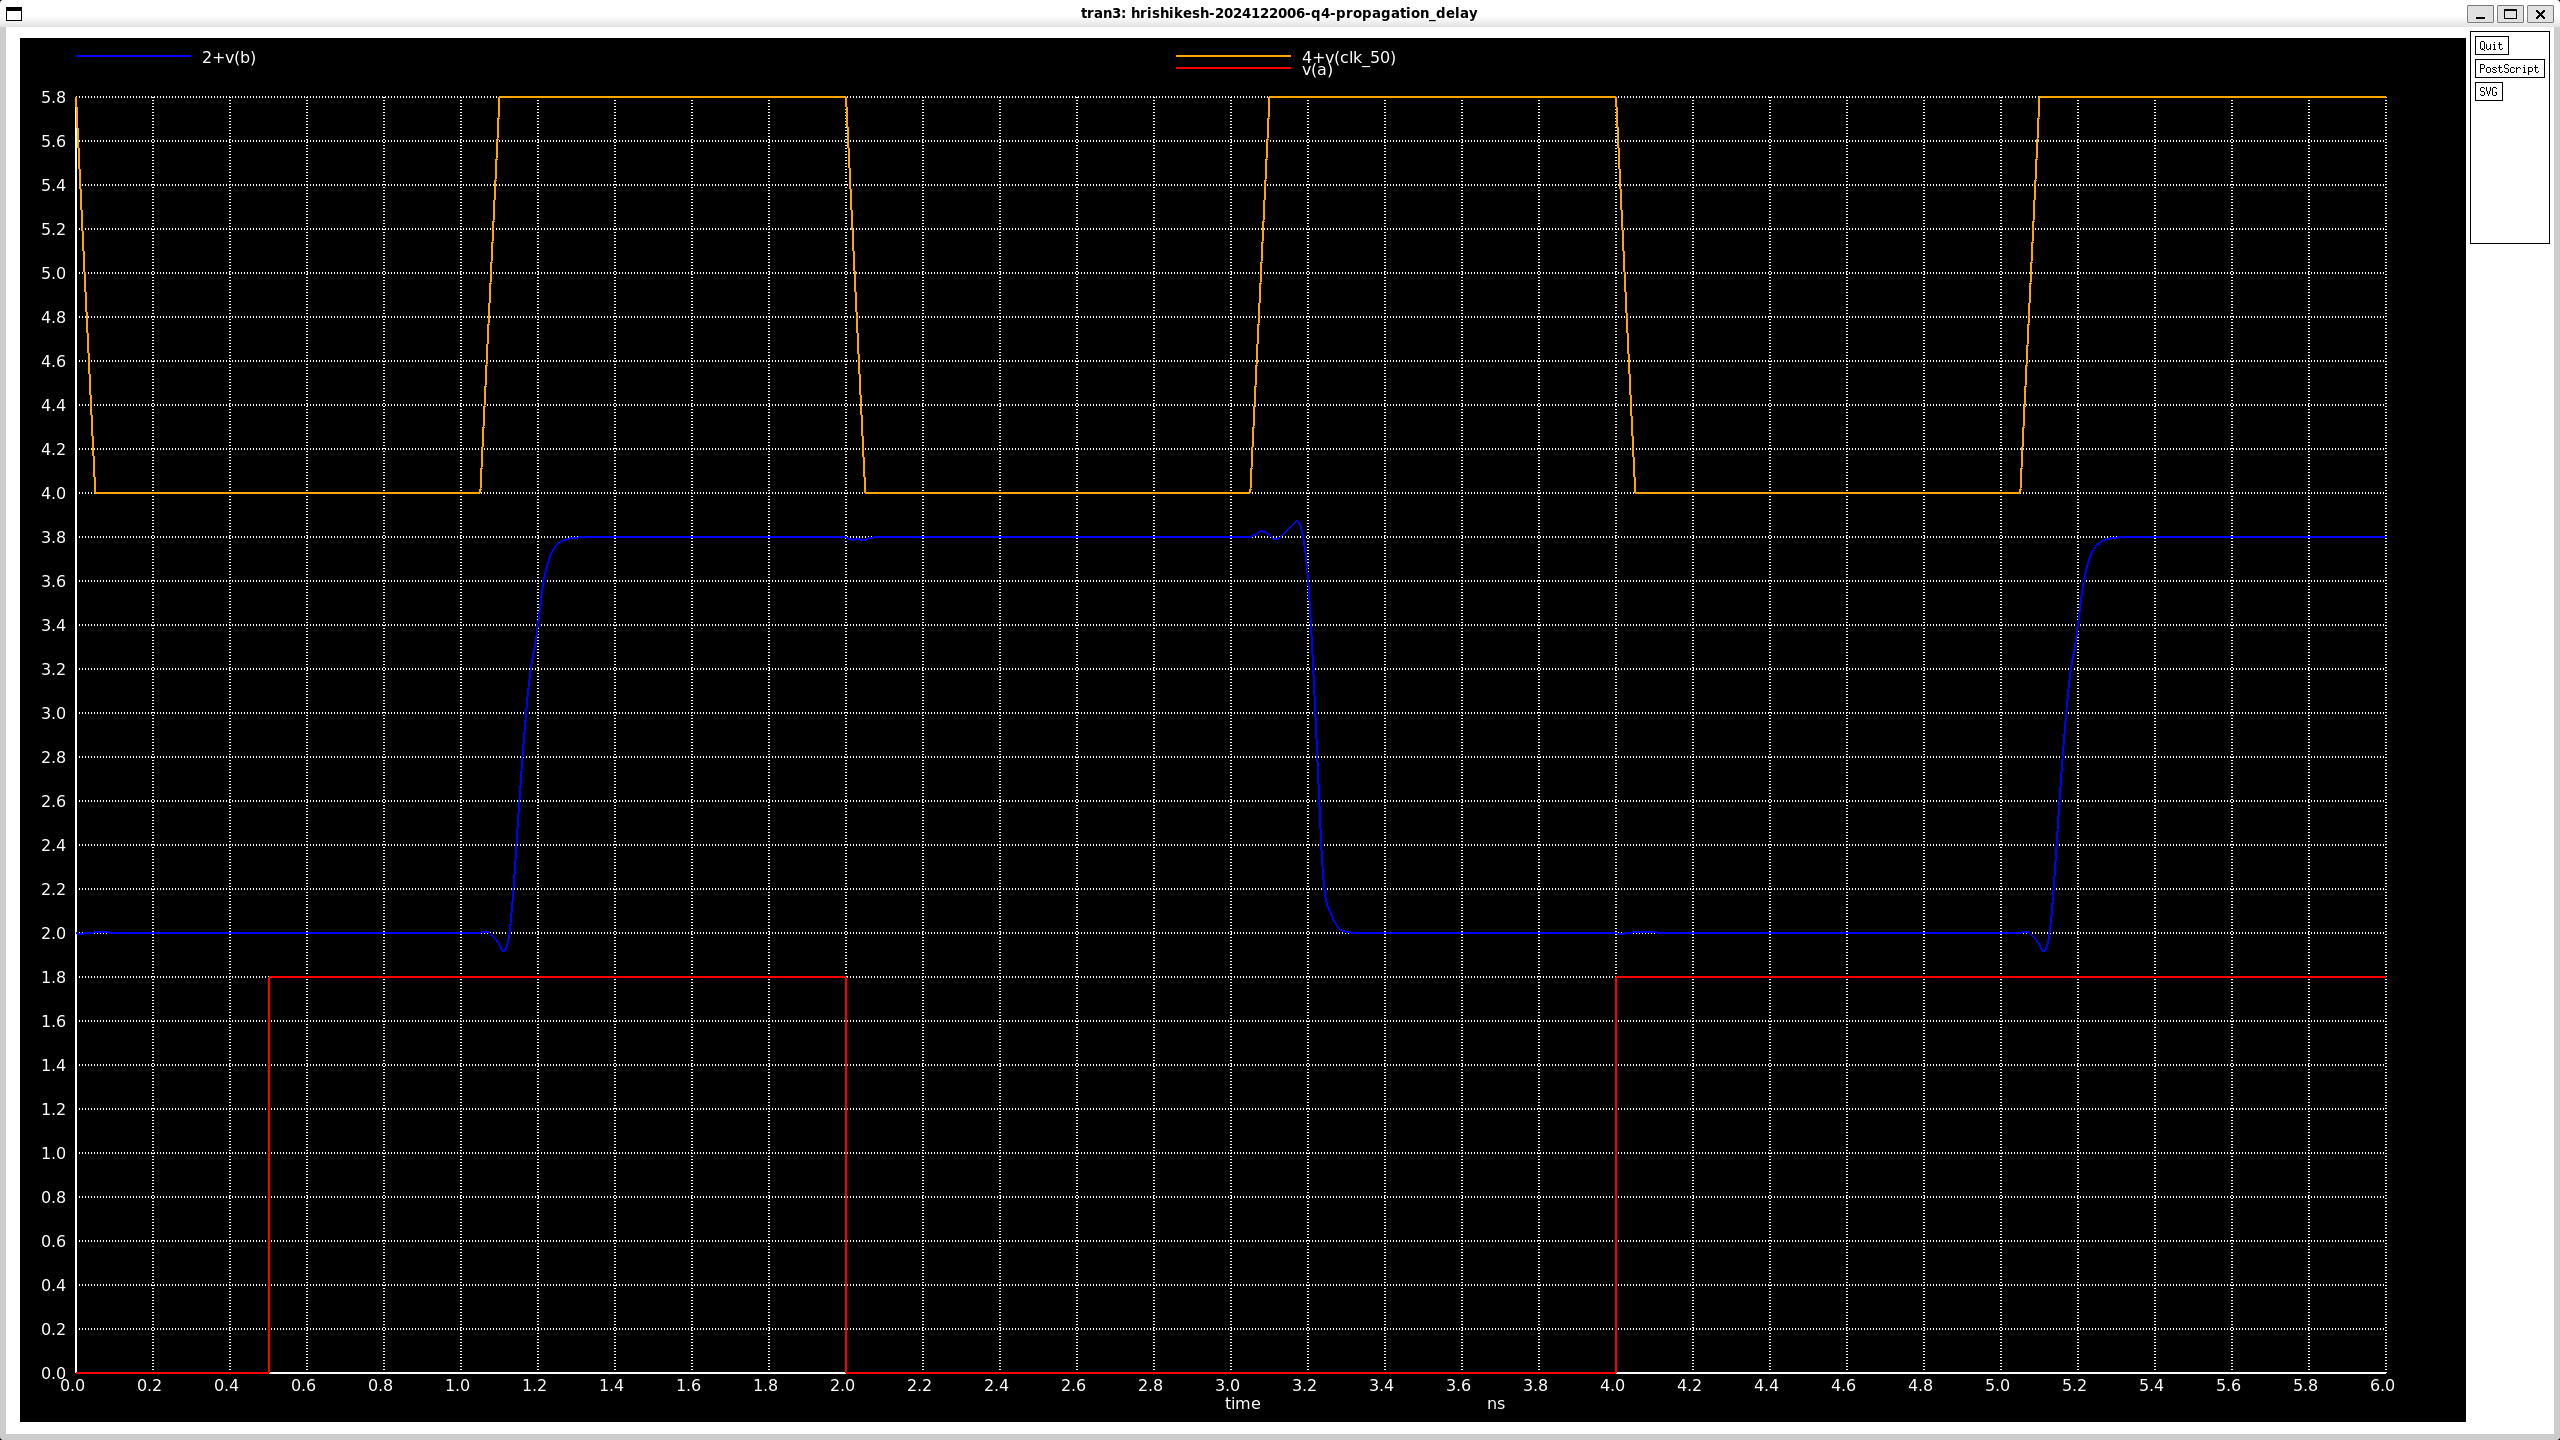
\includegraphics[width=1\linewidth]{dff_pd.png}
    \caption{DFF Propagation Delay}
    \label{fig:enter-label}
\end{figure}
\begin{figure}[H]
    \centering
    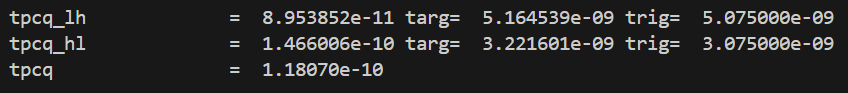
\includegraphics[width=1\linewidth]{pre_tpcq.png}
    \caption{Pre-Layout DFF Propagation Delay}
    \label{fig:enter-label}
\end{figure}
\textbf{Setup Time: }
It is the time period before clock edge before which data should arrive for reliable operation of flip flop. Therefore, to find setup time a very precise (ideal) clock was generated with a rise/fall time of 0 ps. The figure shows the best possible case with minimum setup time possible avoiding any flaws/corruption of output. 
\begin{figure}[H]
    \centering
    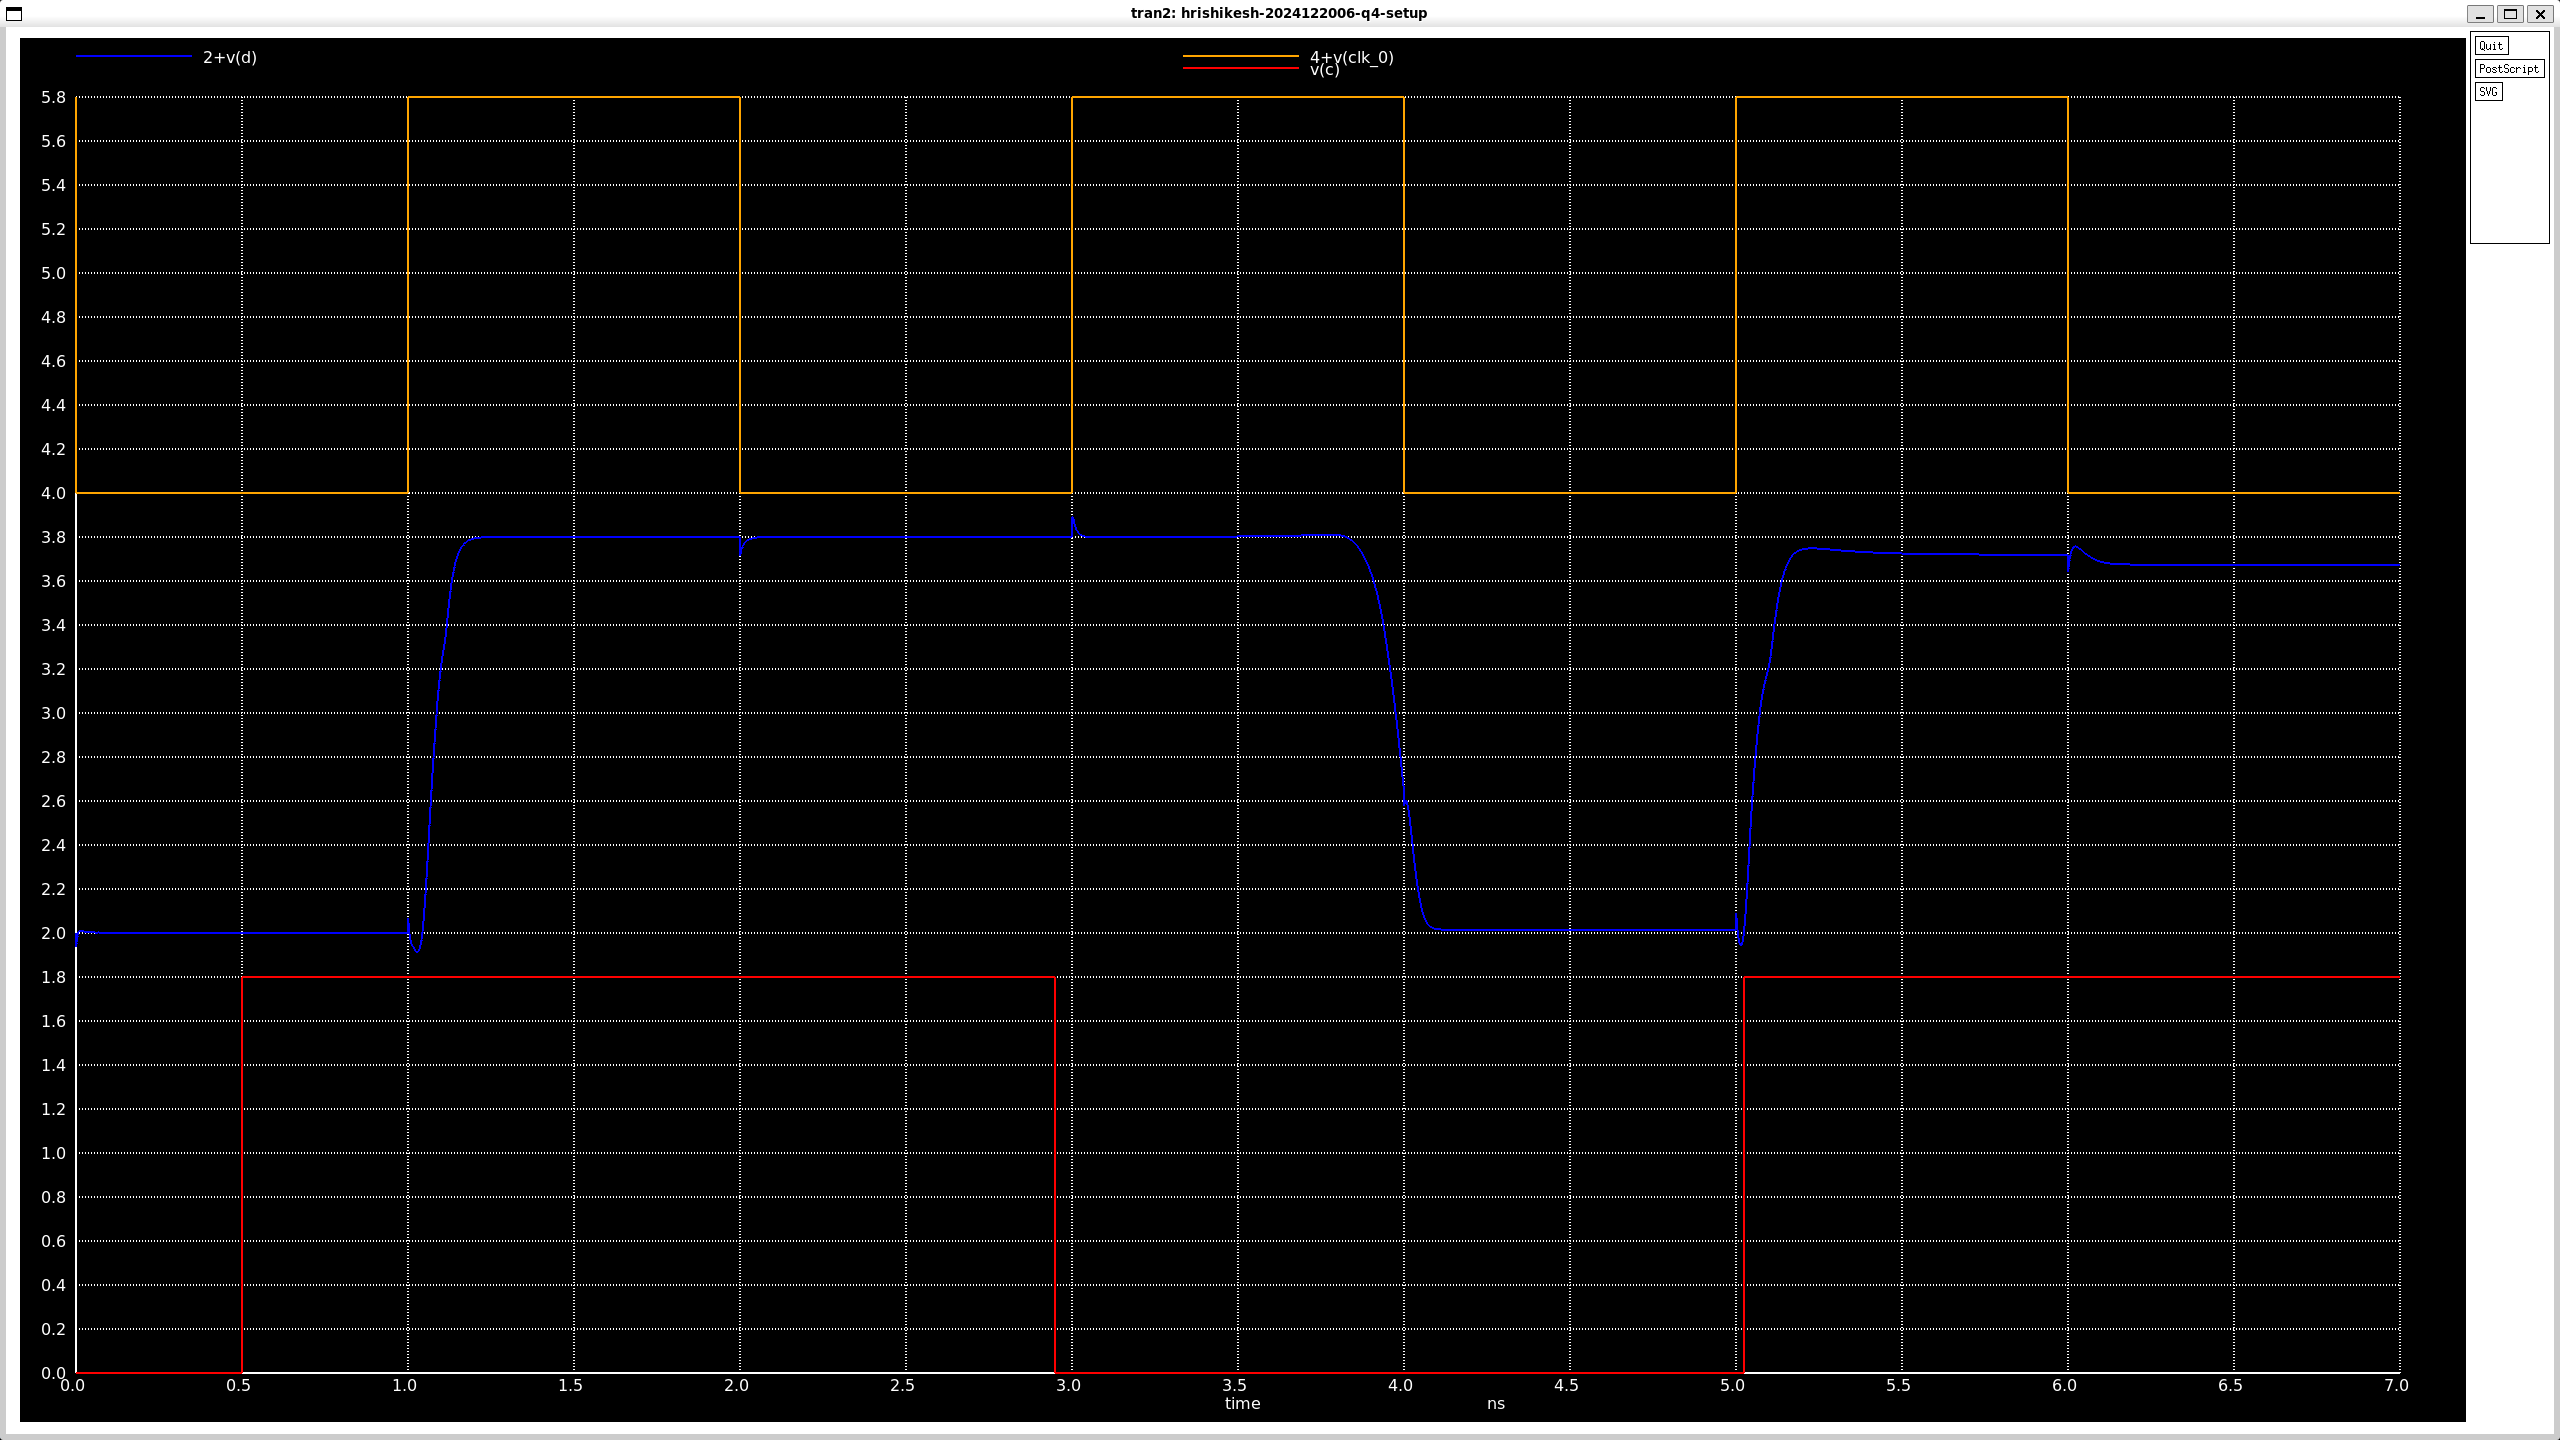
\includegraphics[width=1\linewidth]{pre_setup.png}
    \caption{Setup Time (Best Case)}
    \label{fig:enter-label}
\end{figure}
Any further decrease in results in flaws / data corruption. It was noticed that during low to high case, the output had a flaw. We try to avoid such scenarios when calculating hold and setup time in later parts of report to find the best possible results.
\begin{figure}[H]
    \centering
    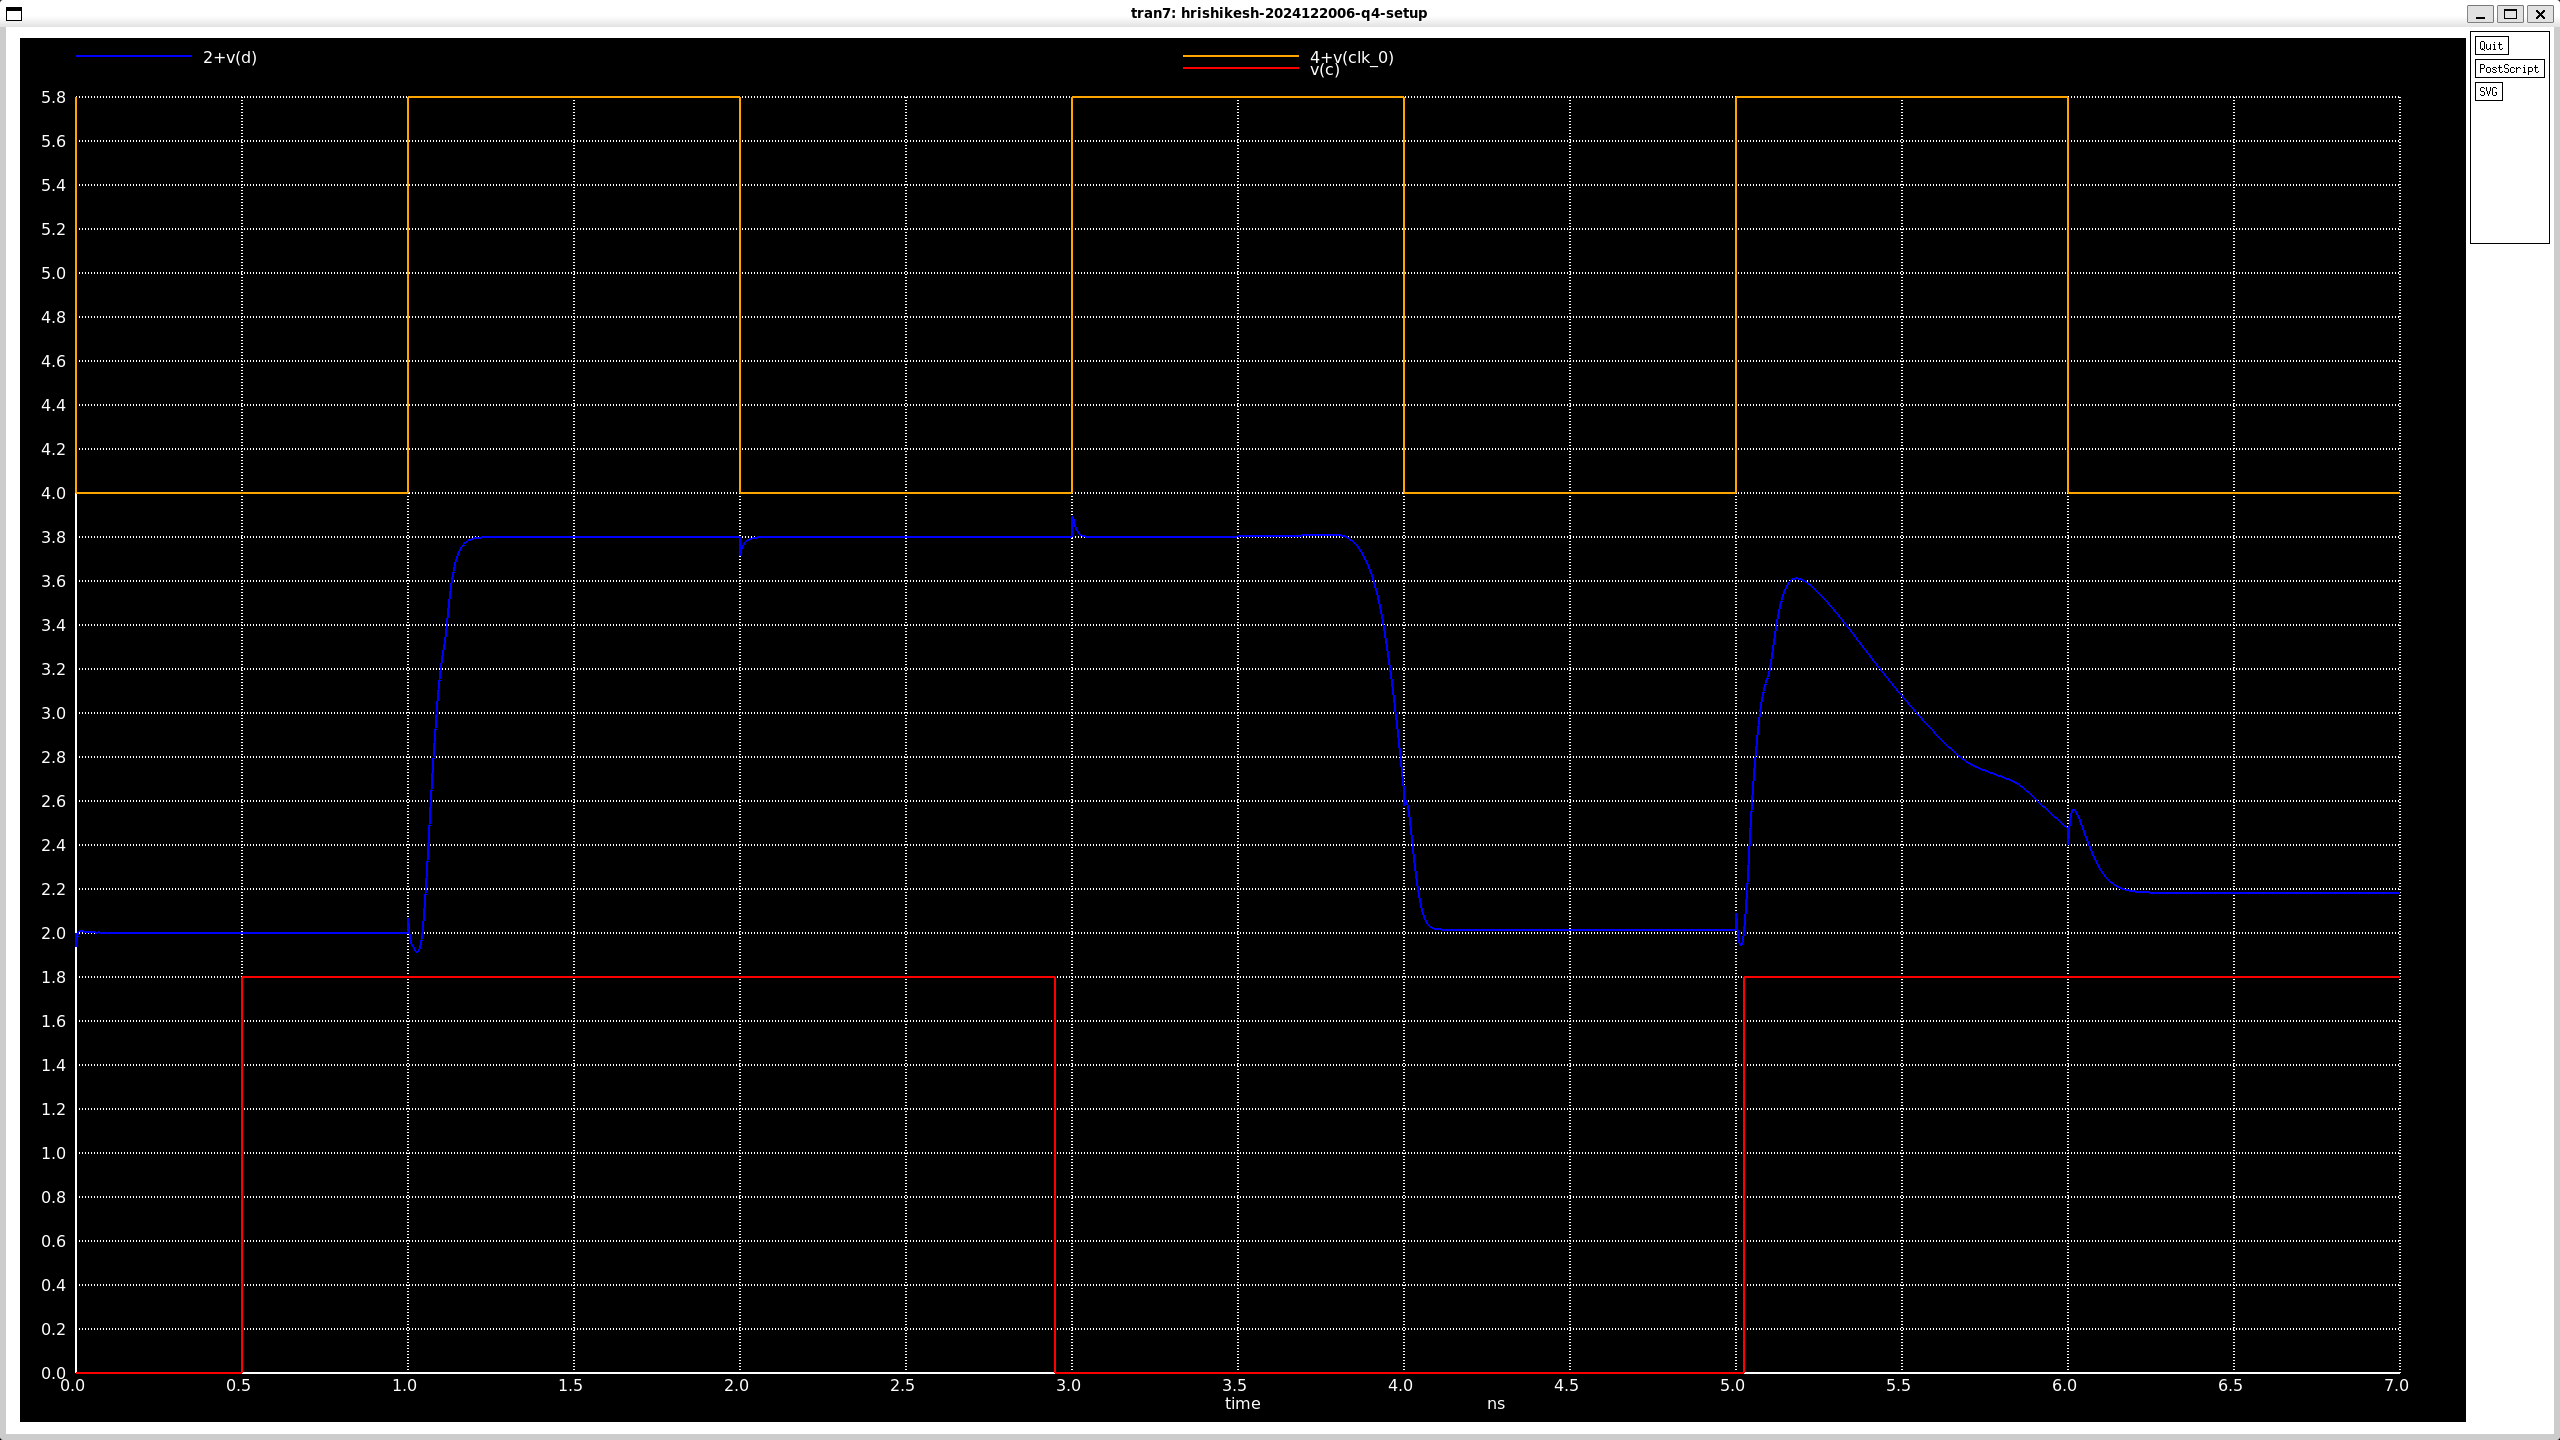
\includegraphics[width=1\linewidth]{pre_setup_flaw.png}
    \caption{Low to High Flaw}
    \label{fig:enter-label}
\end{figure}
\textbf{Hold Time: }
It is the time period after clock edge until which data should remain available for reliable operation of flip flop. Therefore, to find hold time a very precise (ideal) clock was generated with a rise/fall time of 0 ps. The figure shows the best possible case with minimum hold time possible avoiding any flaws/corruption of output. 
\begin{figure}[H]
    \centering
    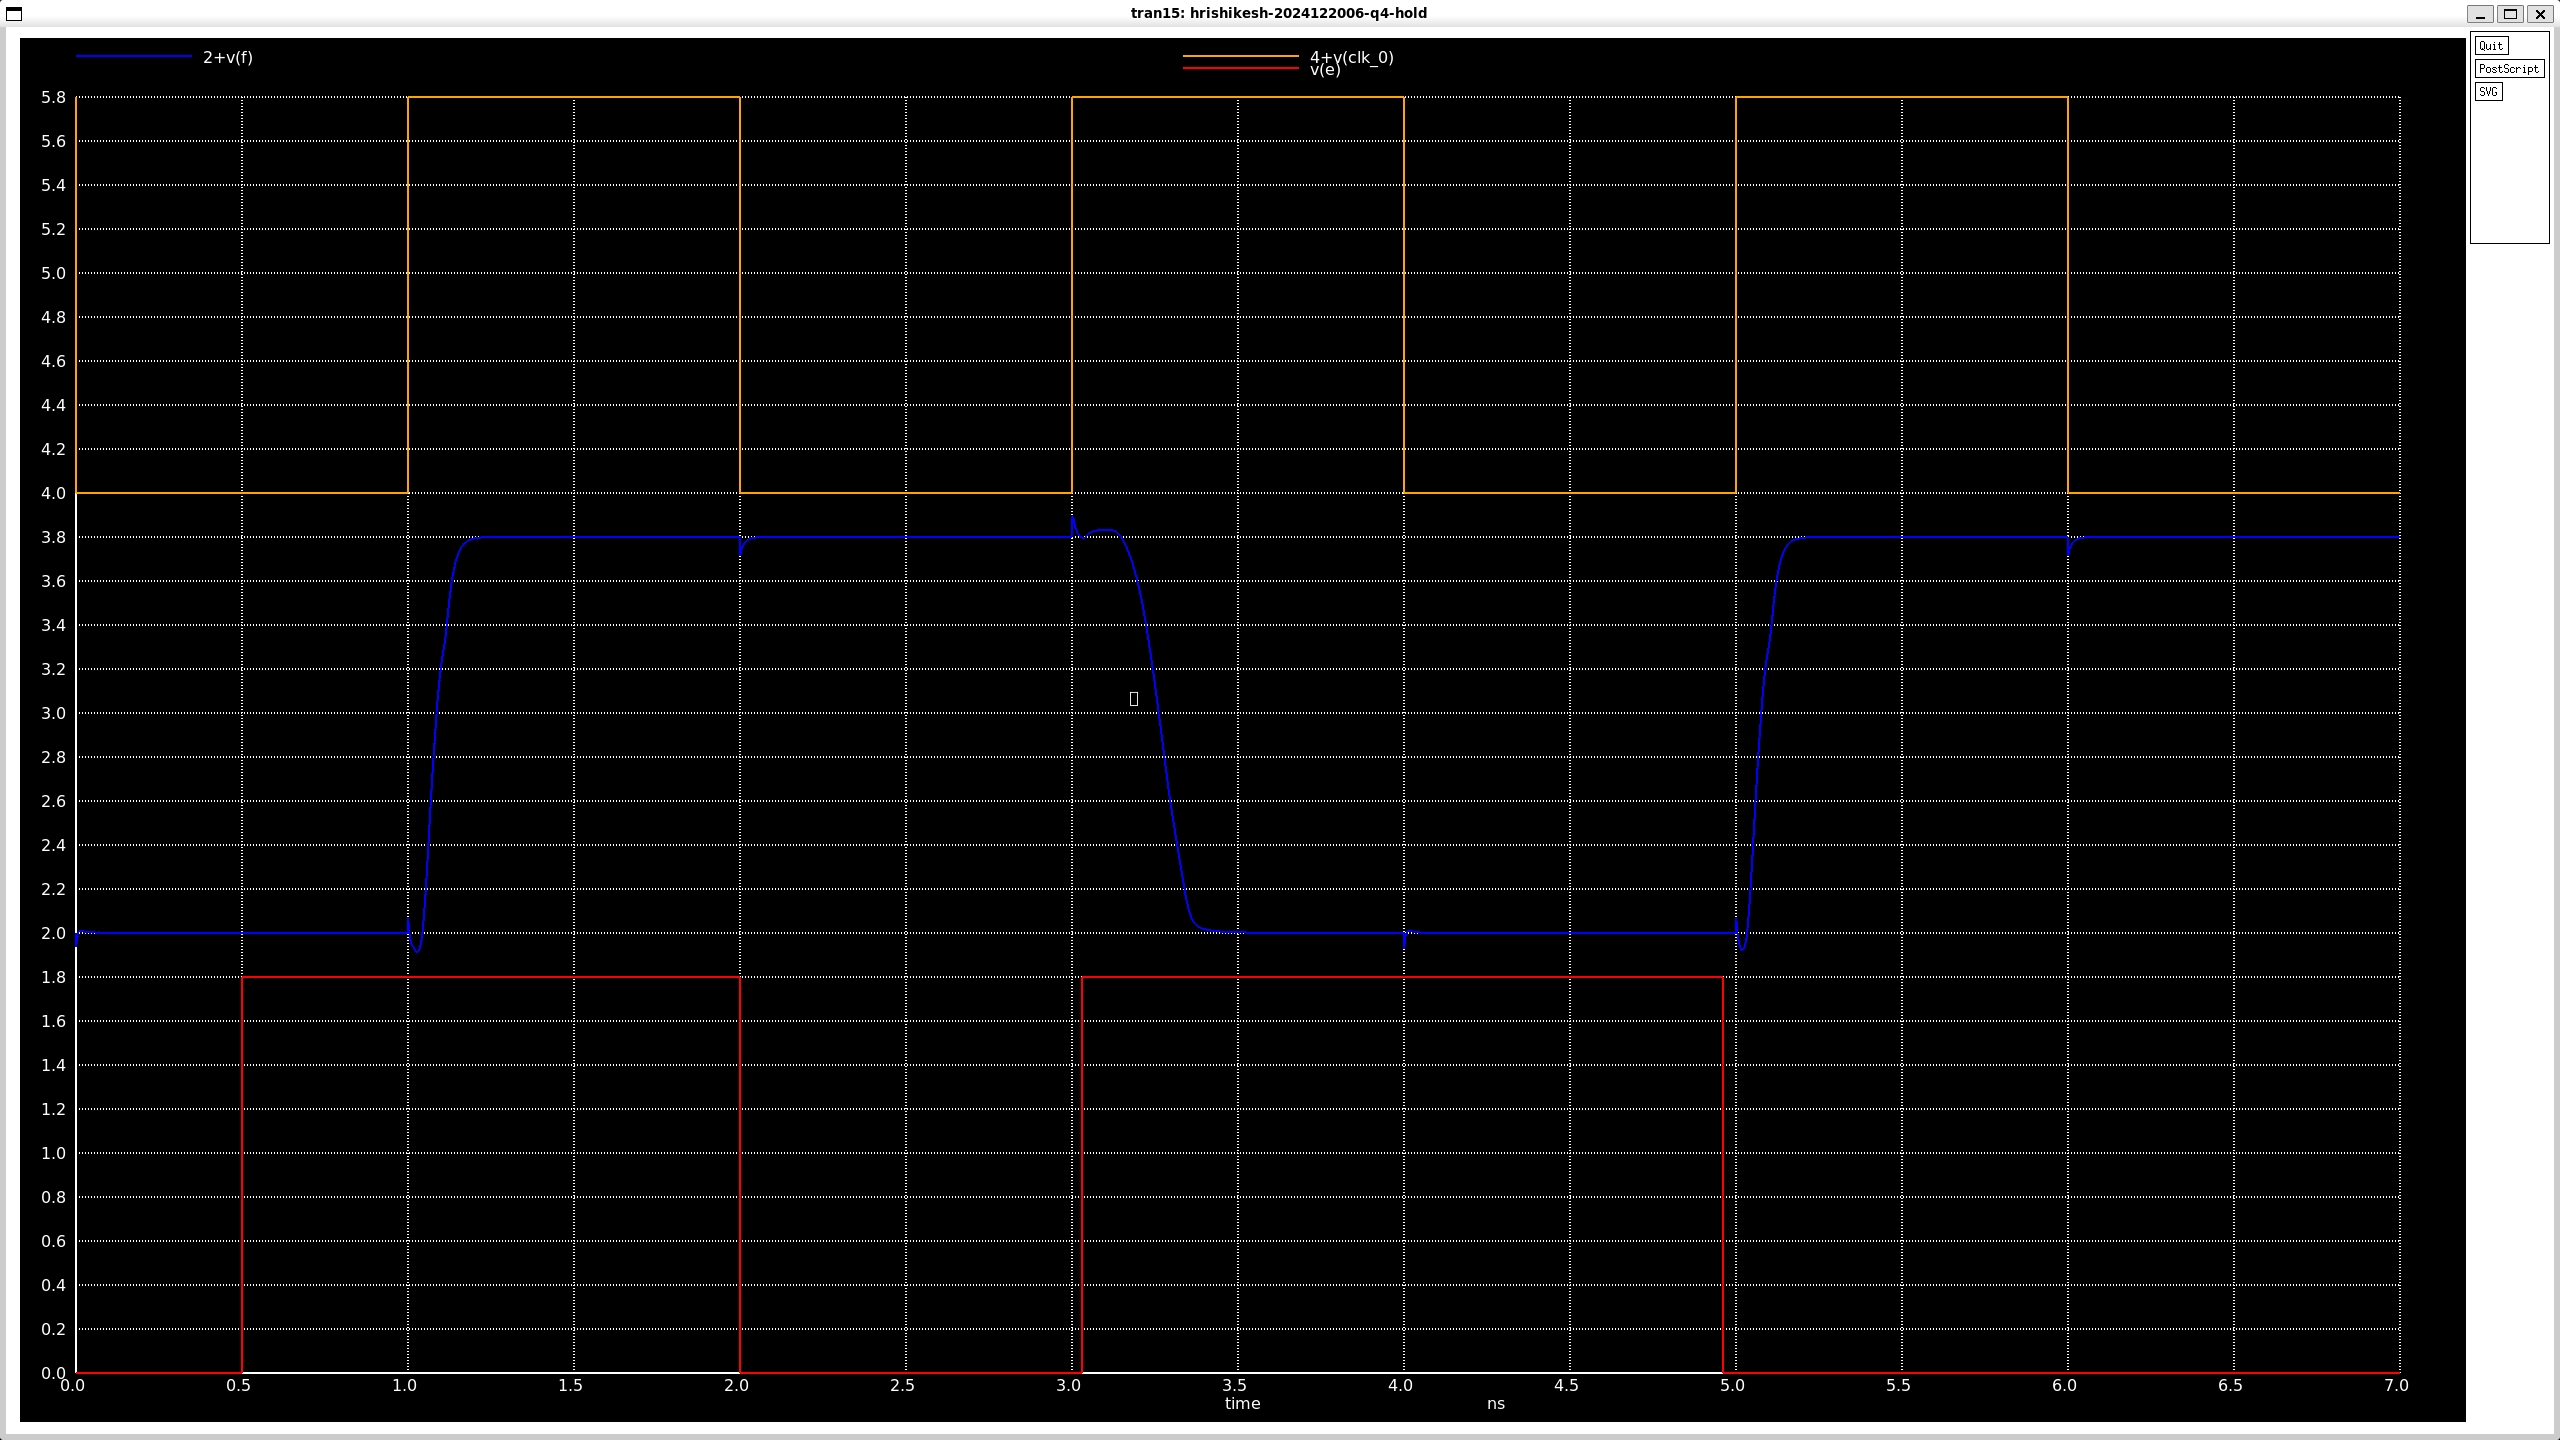
\includegraphics[width=1\linewidth]{pre_hold.png}
    \caption{Hold Time (Best Case)}
    \label{fig:enter-label}
\end{figure}
Decreasing this hold time for high to low case increases $t_p$ which is not suitable for reliable operation of cla at high frequency.
\begin{figure}[H]
    \centering
    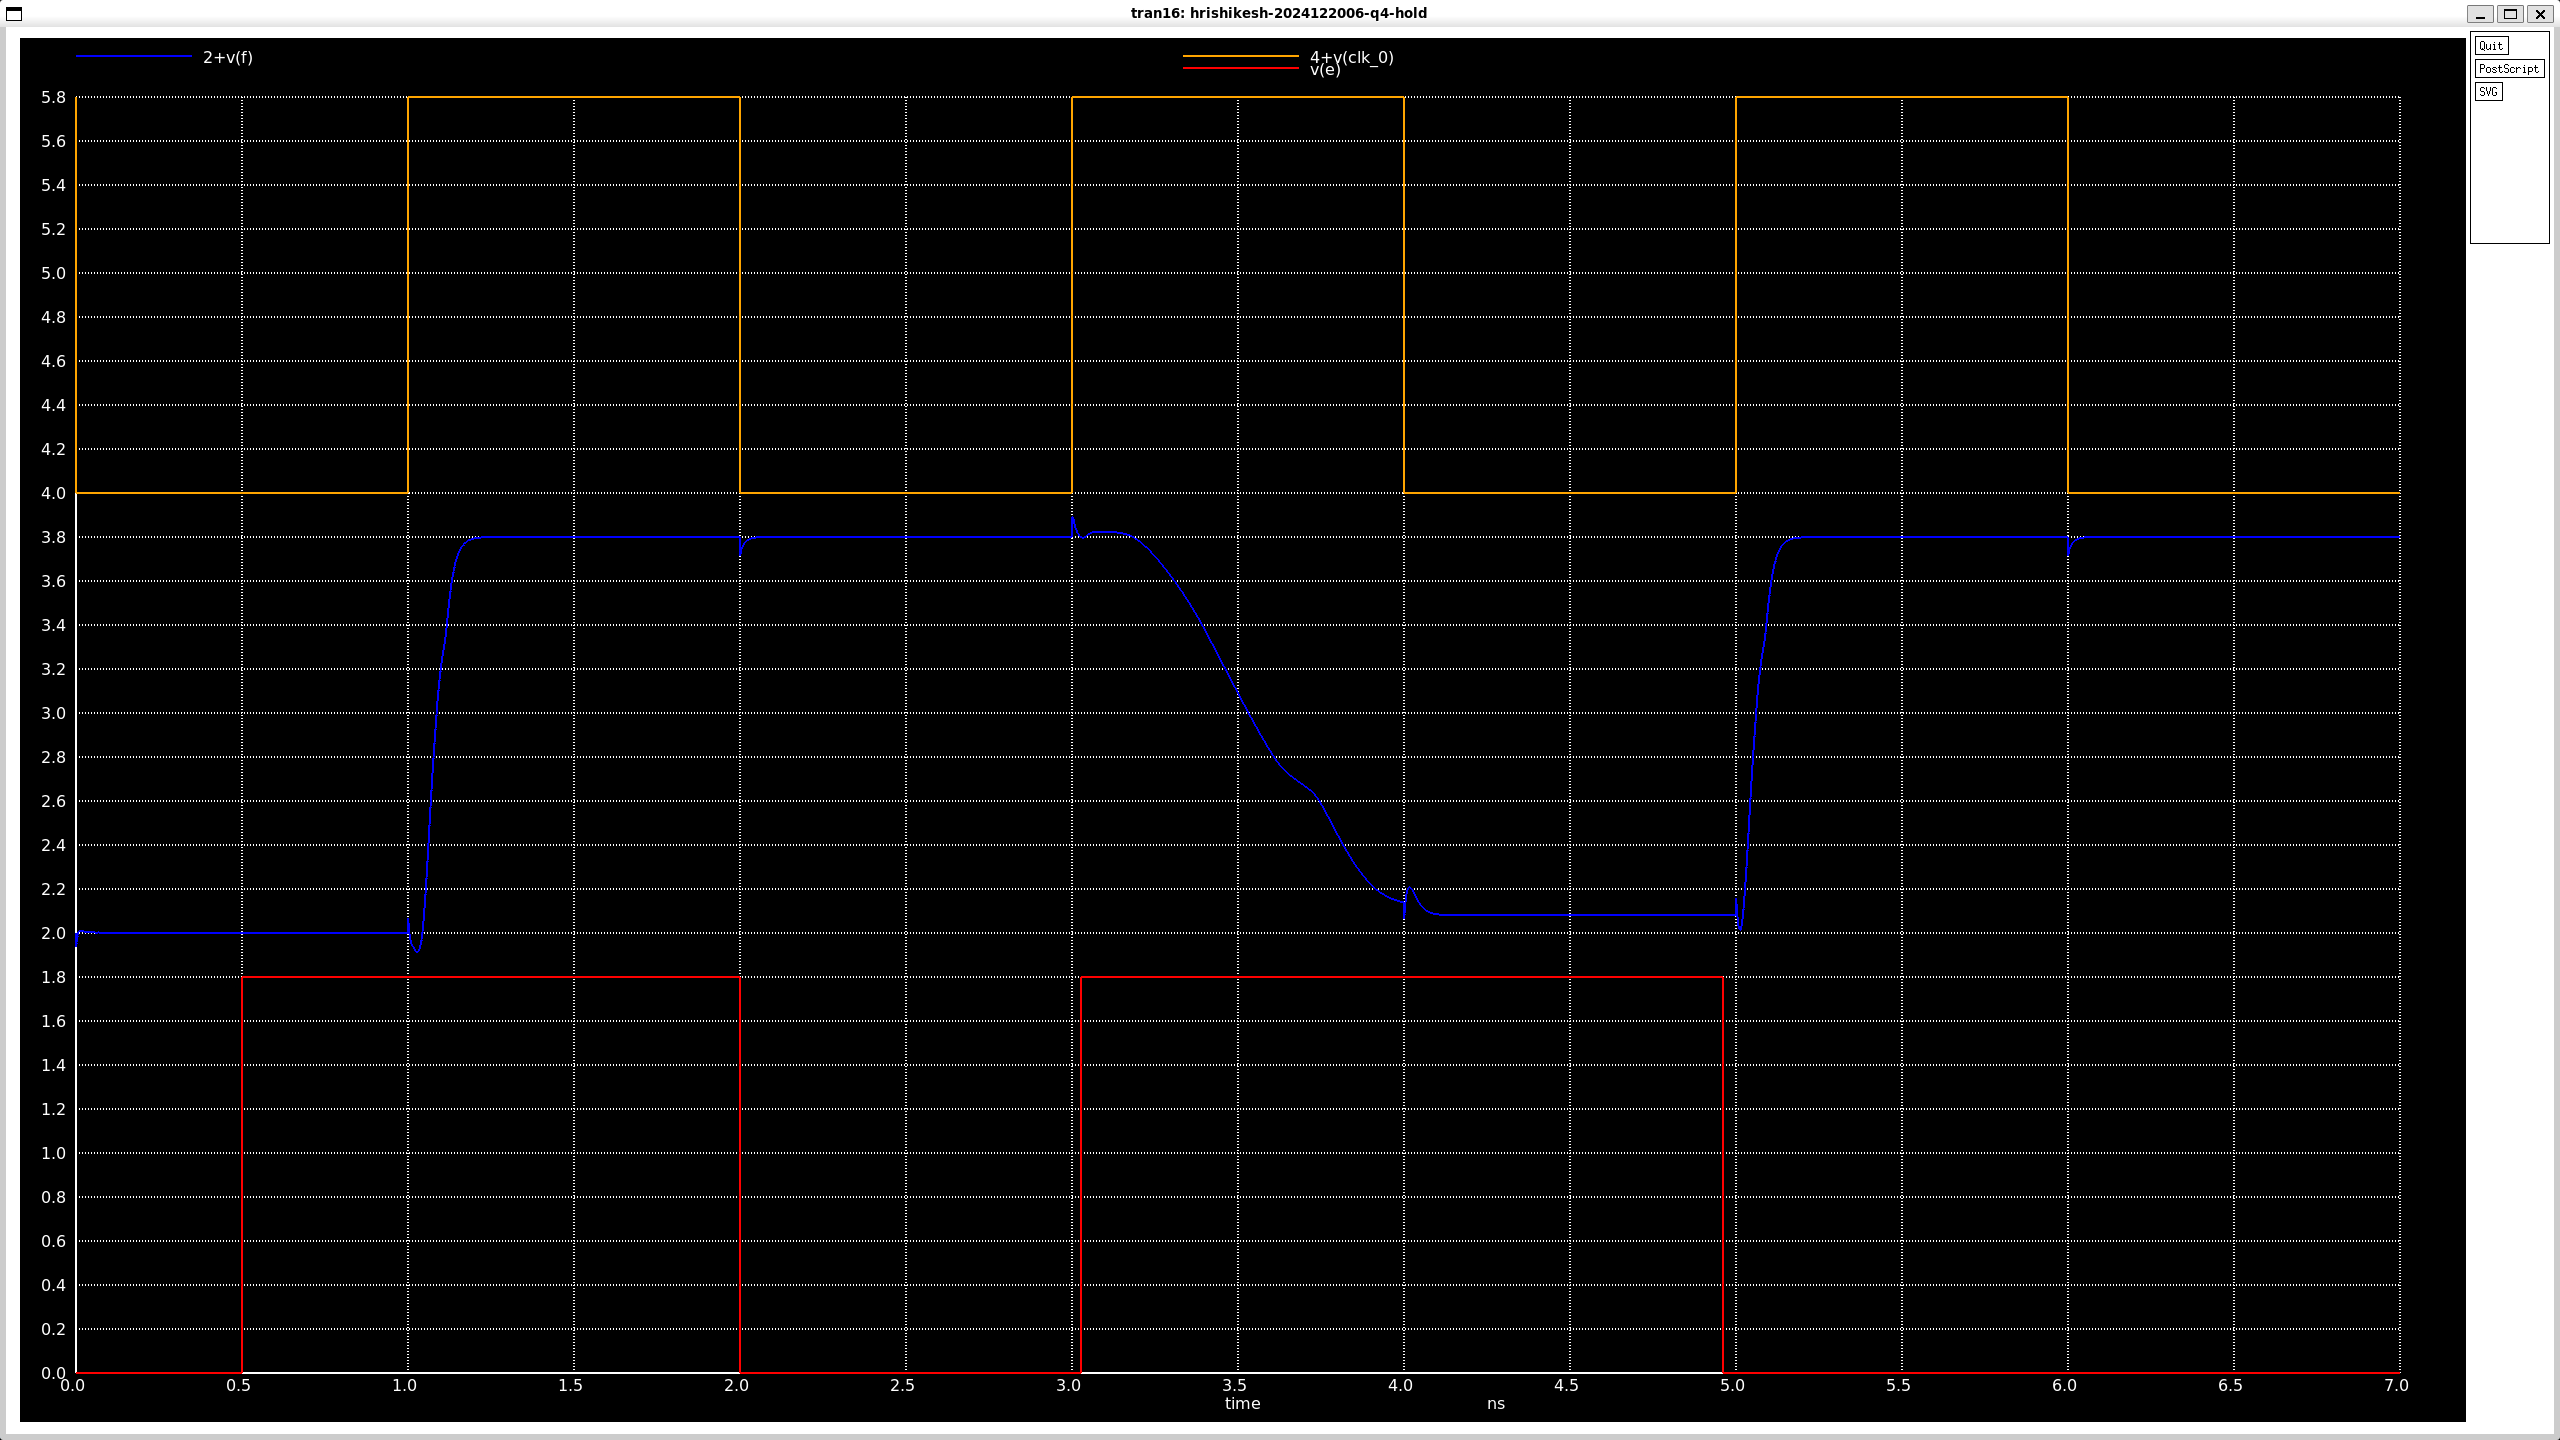
\includegraphics[width=1\linewidth]{pre_hold_flaw.png}
    \caption{High to Low Flaw}
    \label{fig:enter-label}
\end{figure}
Timing Parameters for a Pre-Layout D Flip-Flop are shown below.
\begin{center}
\begin{tabular}{|c|c|c|c|}
\hline
\textbf{Transition} & \boldmath$t_{\text{setup}}$ & \boldmath$t_{\text{hold}}$ & \boldmath$t_p$ \\ \hline
Low to High & 24 ps * & 40 ps * & 8.953852e-11 s \\ \hline
High to Low & 50 ps & 30 ps & 1.466006e-10 s \\ \hline
Final & 50 ps & 30 ps & 1.18070e-10 s \\ \hline
\end{tabular}
\end{center}
* denotes time post clock edge for $t_{setup}$ and prior clock edge for $t_{hold}$. Finally, we consider the maximum time before clock edge for setup and maximum time after clock edge for hold time. Also average propagation delay is found and noted.
\section{Stick Diagrams}
\begin{figure}[H]
    \centering
    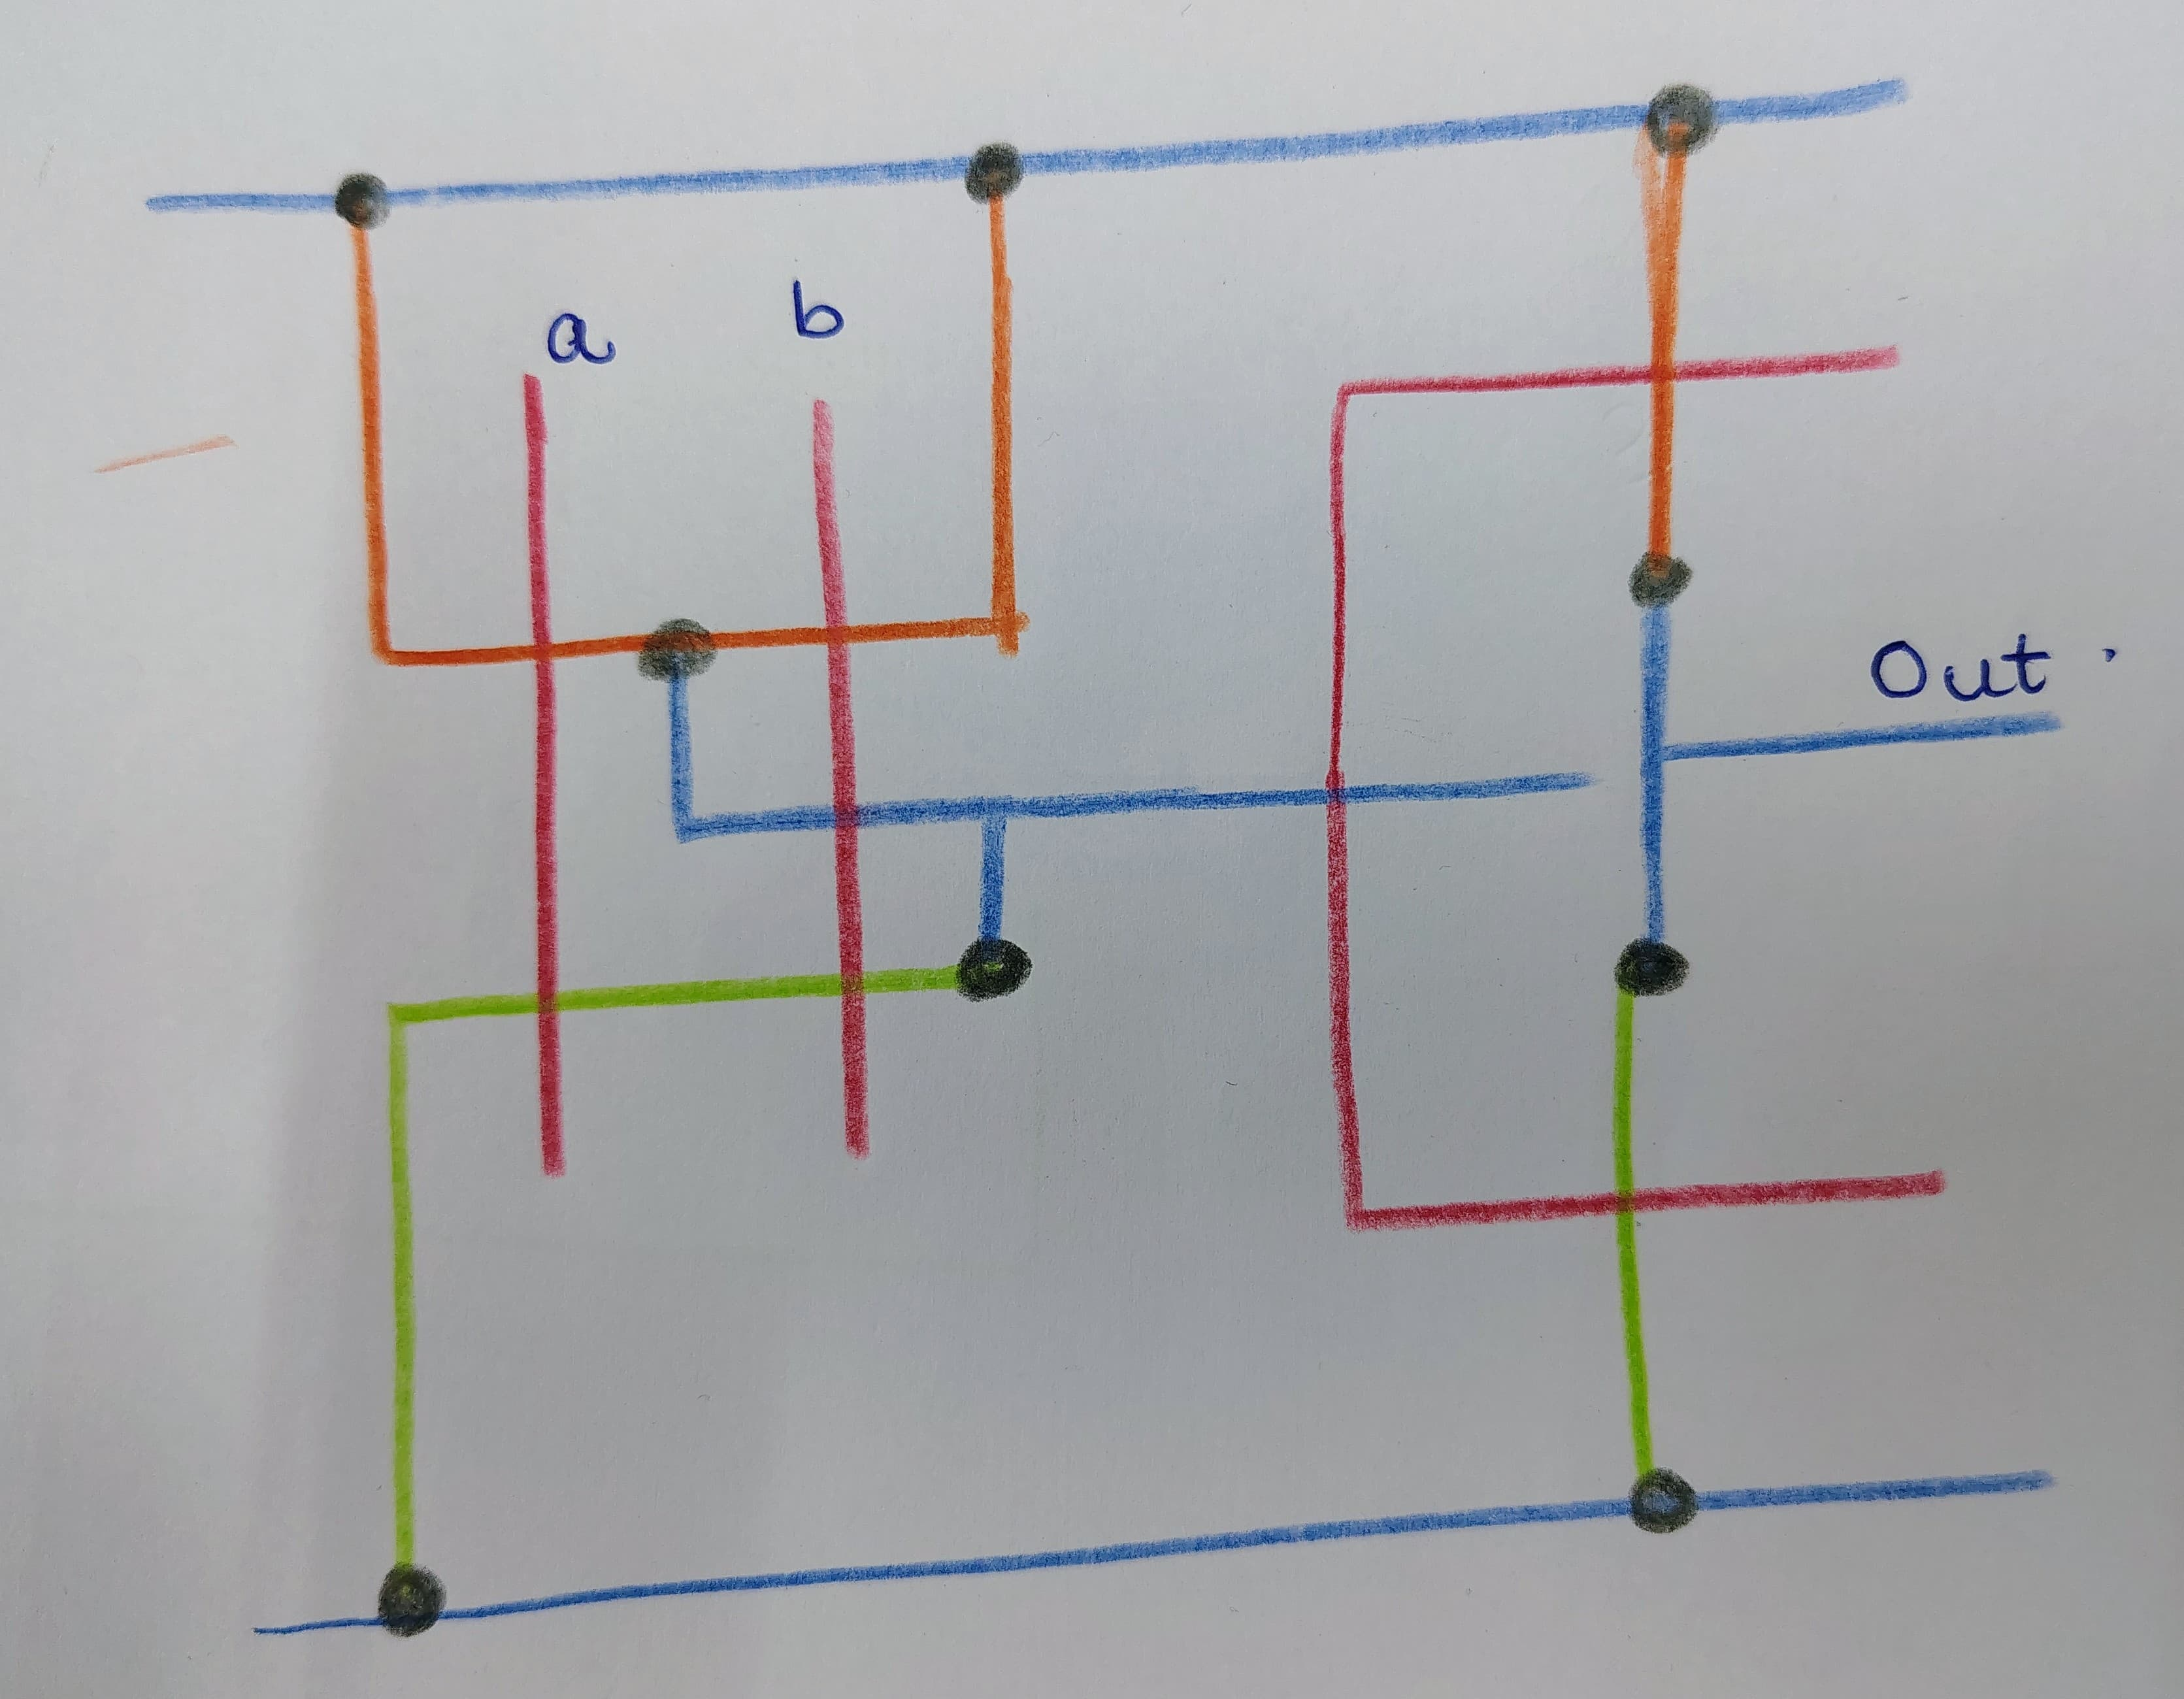
\includegraphics[width=1\linewidth]{stick_and.jpg}
    \caption{AND Gate}
    \label{fig:enter-label}
\end{figure}
\begin{figure}[H]
    \centering
    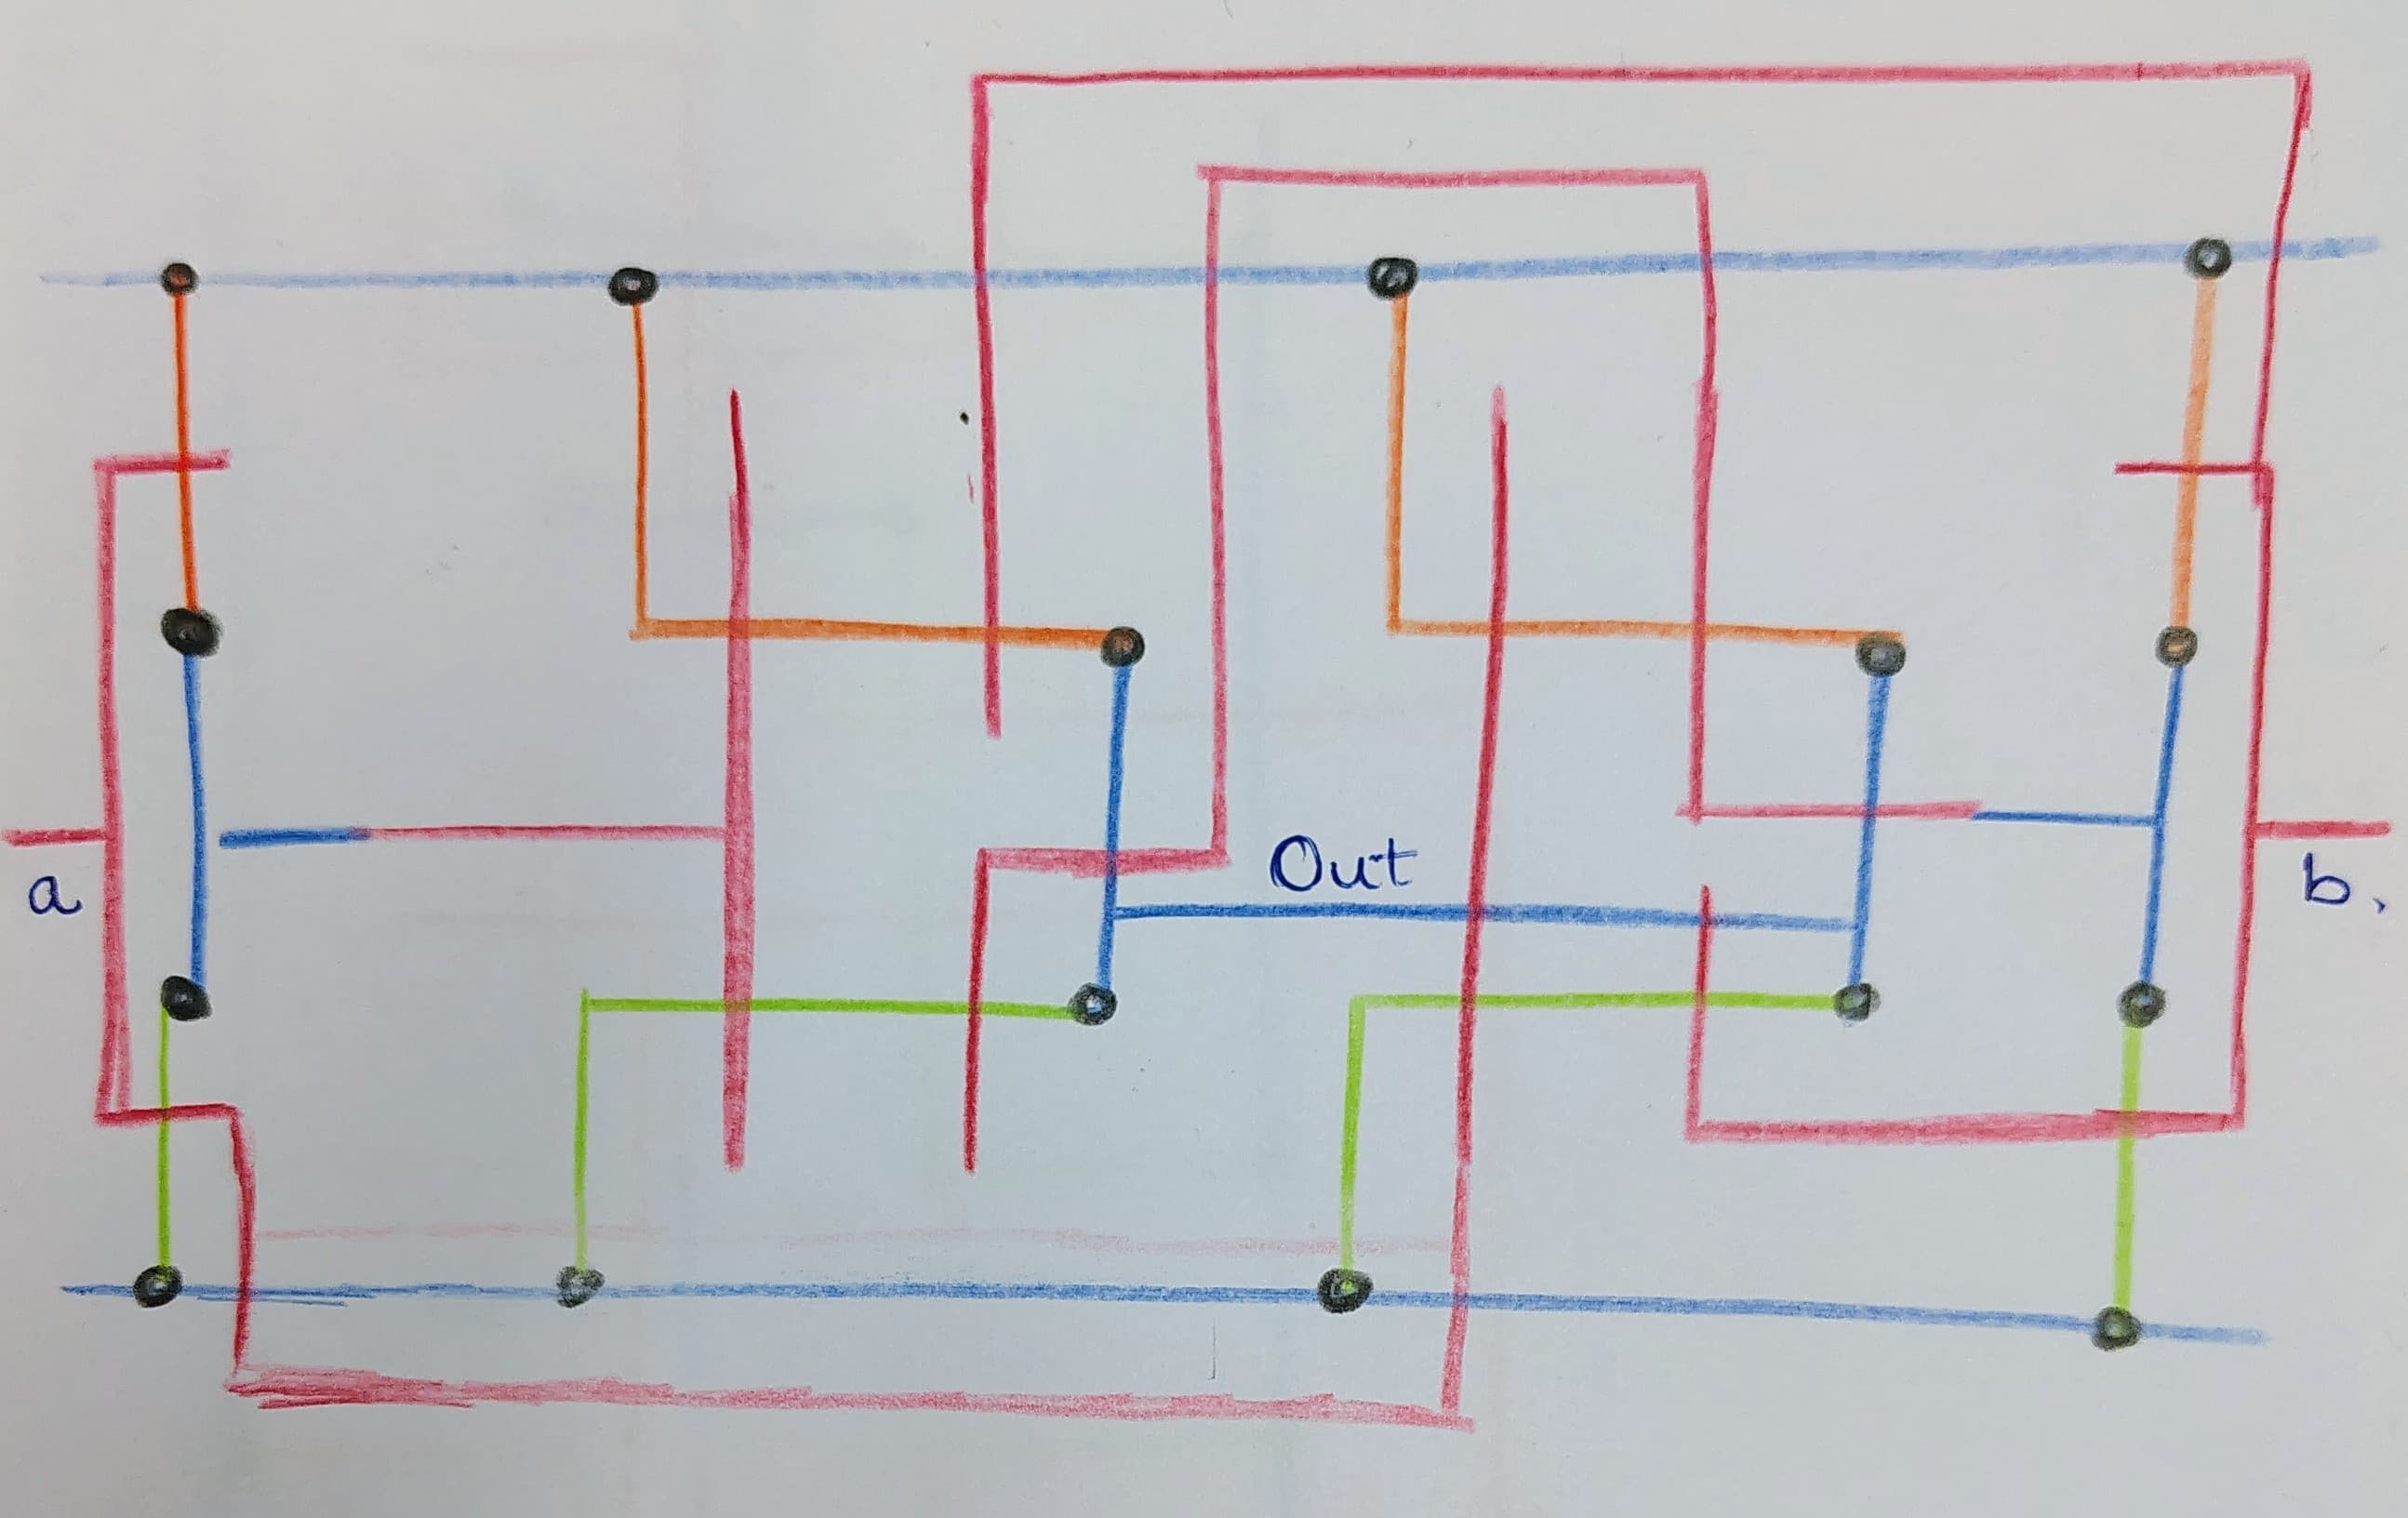
\includegraphics[width=1\linewidth]{stick_xor.jpg}
    \caption{XOR Gate}
    \label{fig:enter-label}
\end{figure}
\begin{figure}[H]
    \centering
    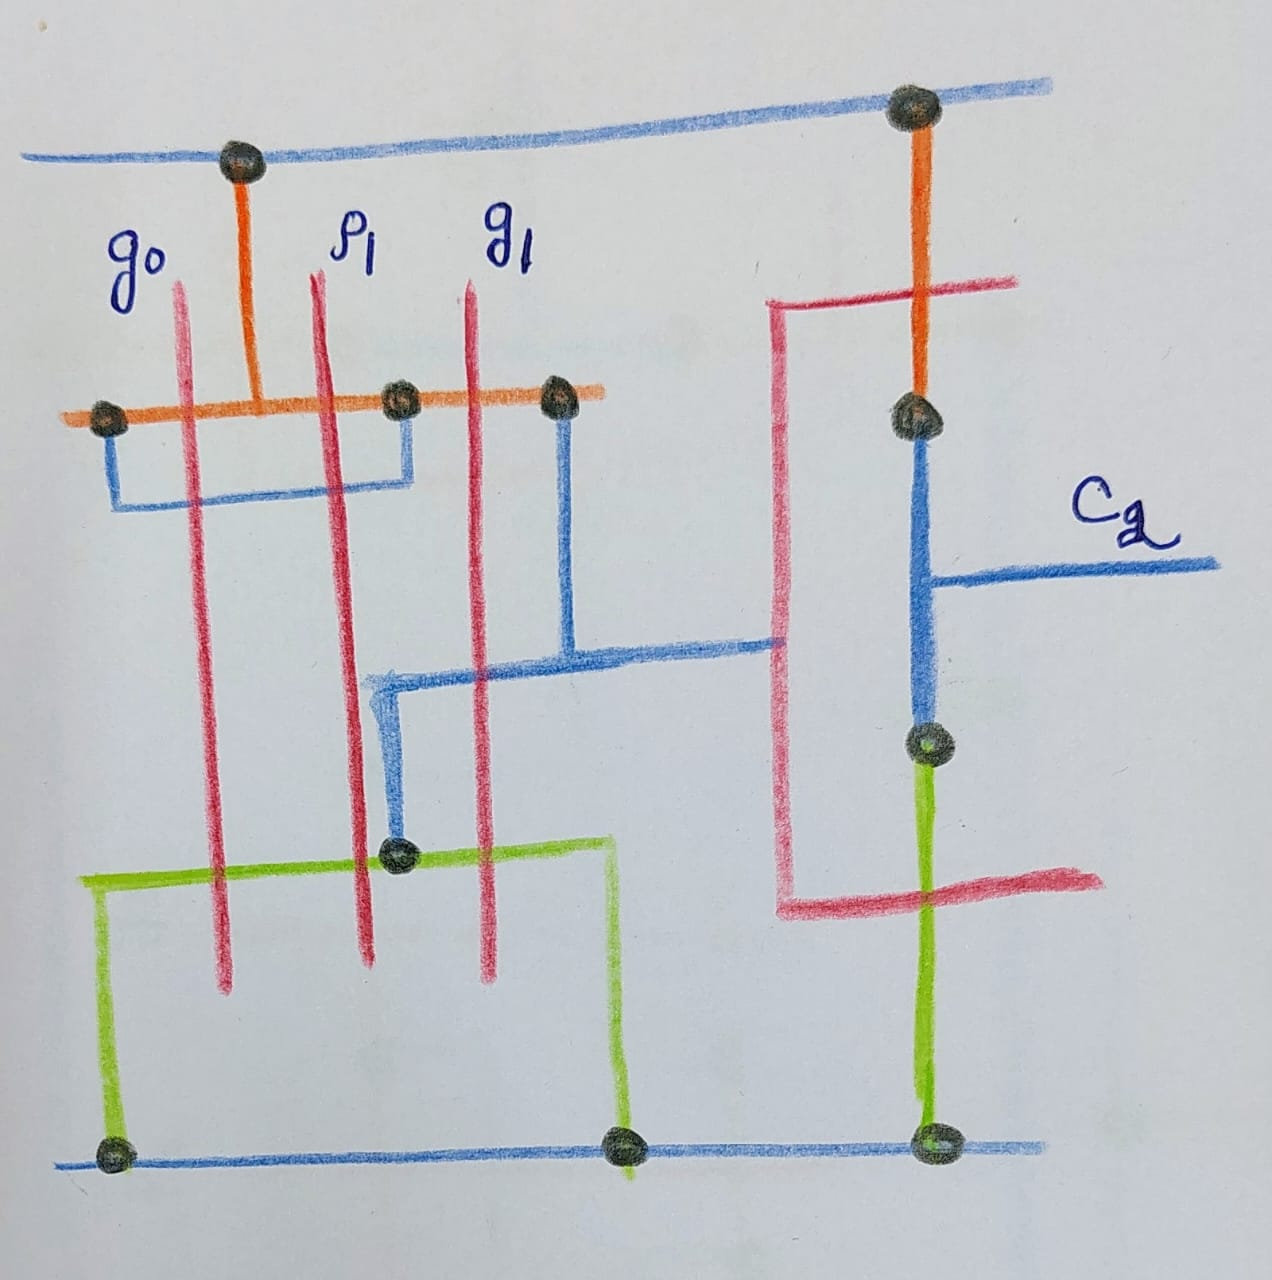
\includegraphics[width=1\linewidth]{stick_c2.jpg}
    \caption{C2 Logic}
    \label{fig:enter-label}
\end{figure}
\begin{figure}[H]
    \centering
    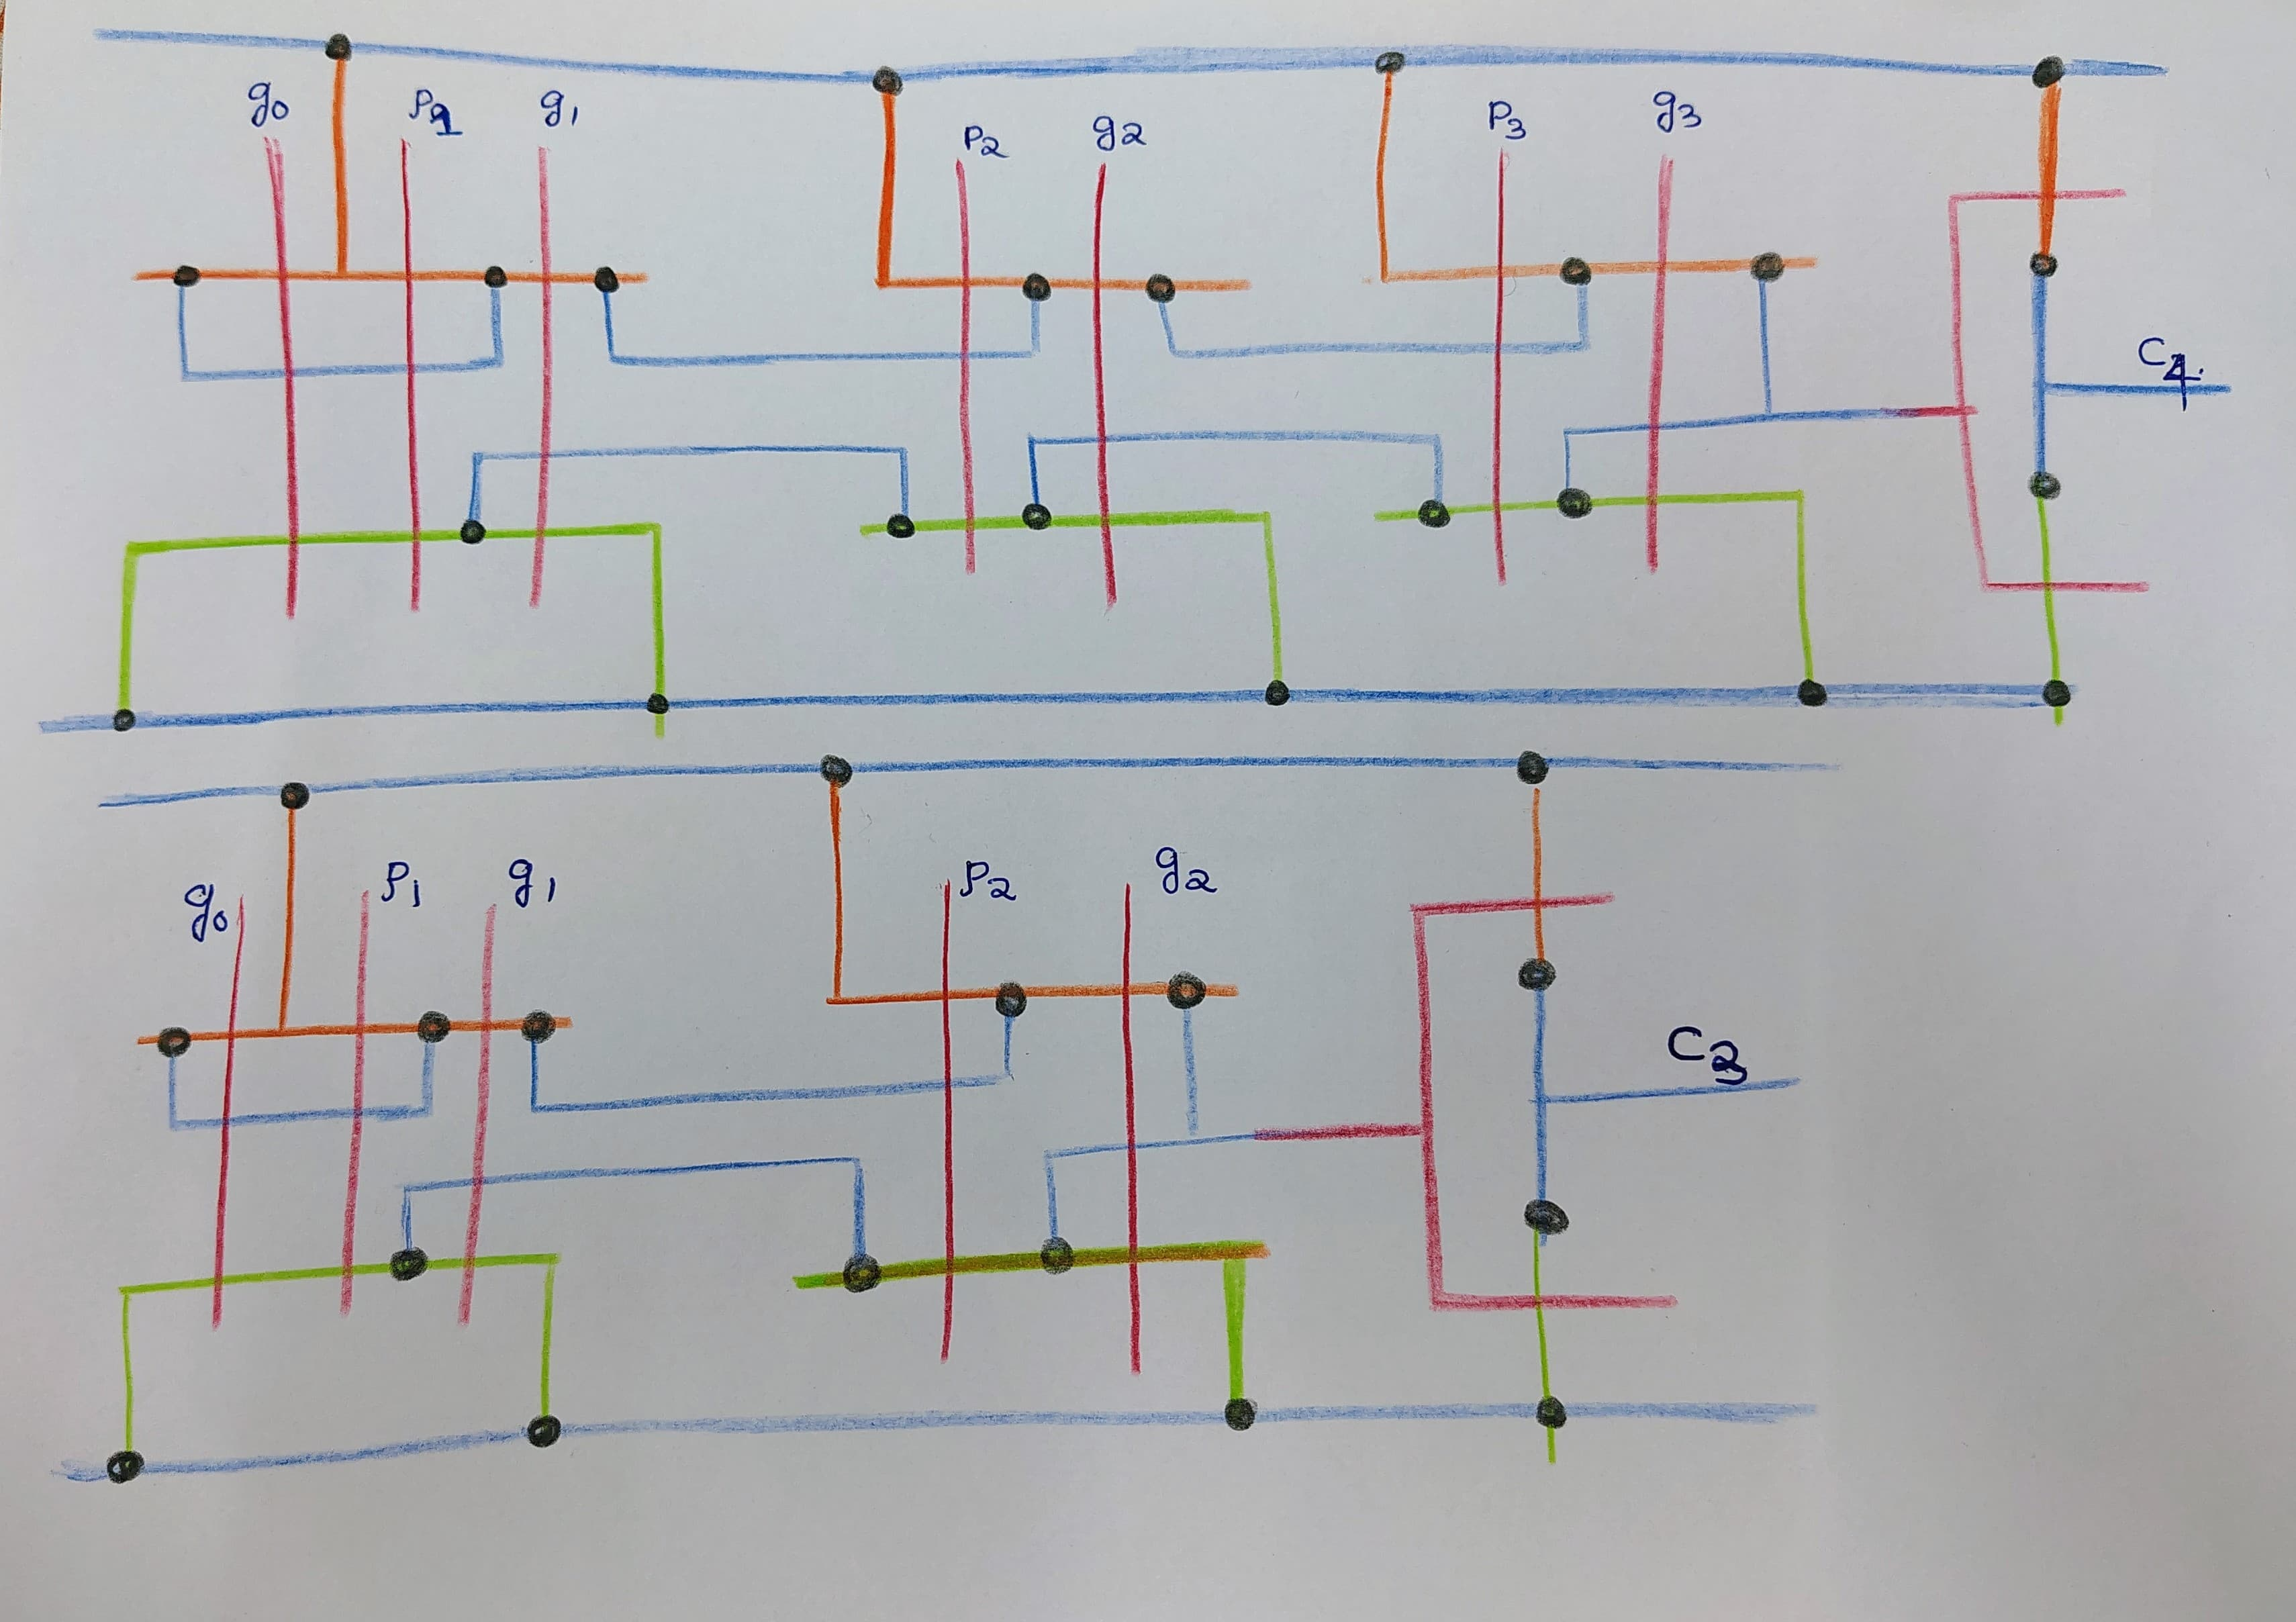
\includegraphics[width=1\linewidth]{stick_c3_c4.jpg}
    \caption{C3 and C4 Logic}
    \label{fig:enter-label}
\end{figure}
\begin{figure}[H]
    \centering
    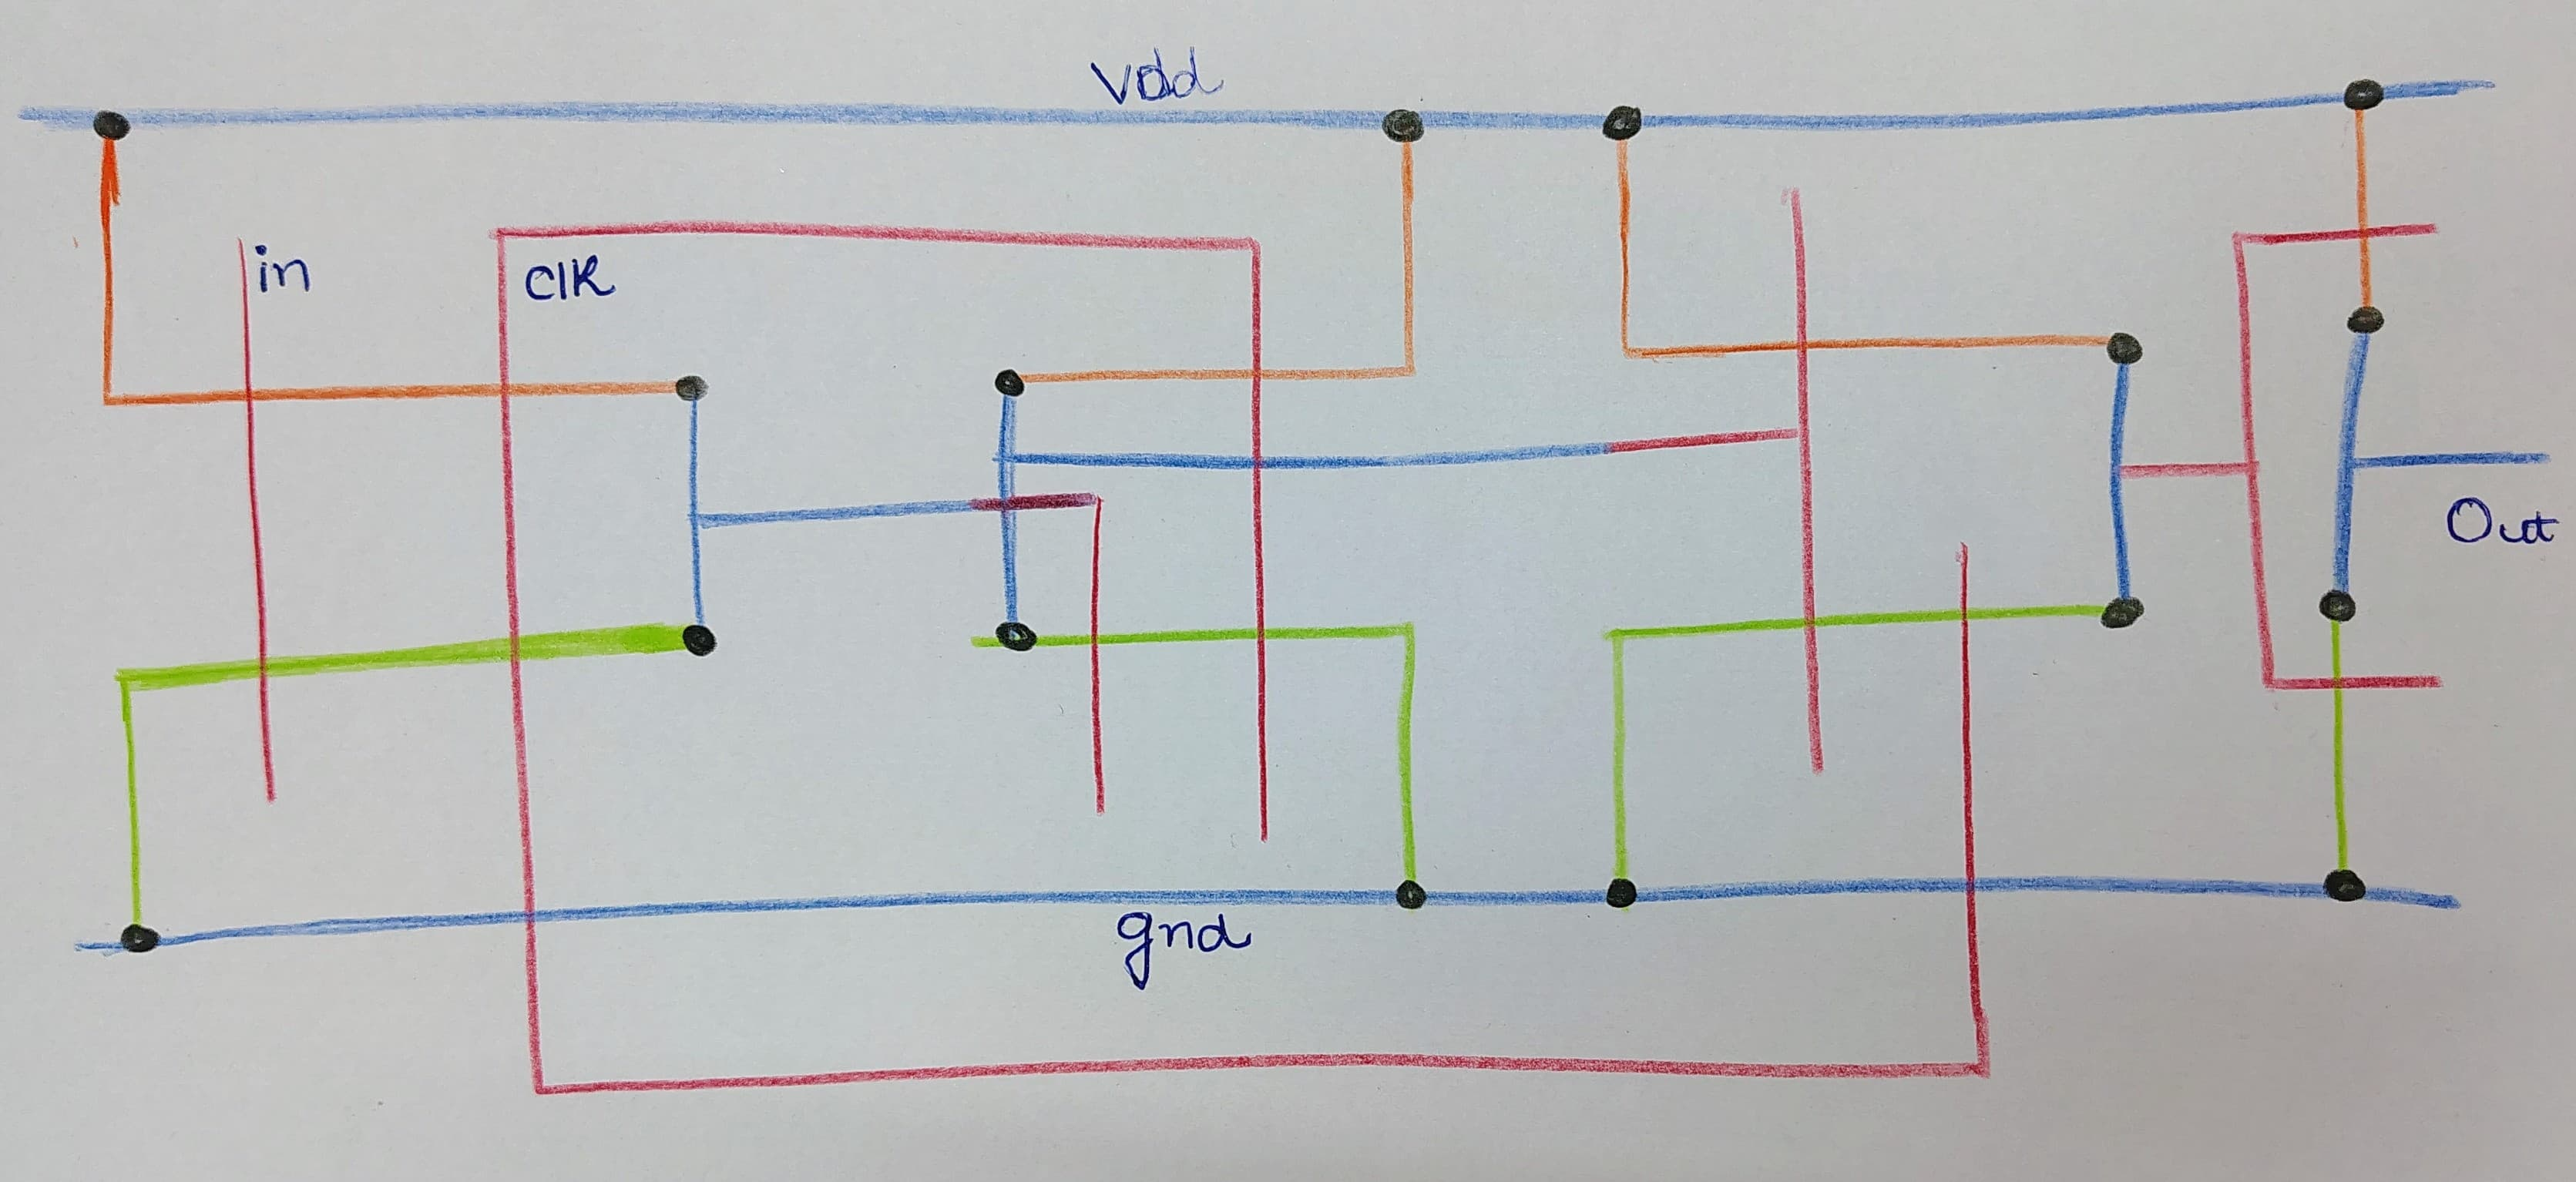
\includegraphics[width=1\linewidth]{stick_dff.jpg}
    \caption{TSPC D Flip Flop}
    \label{fig:enter-label}
\end{figure}
\begin{figure}[H]
    \centering
    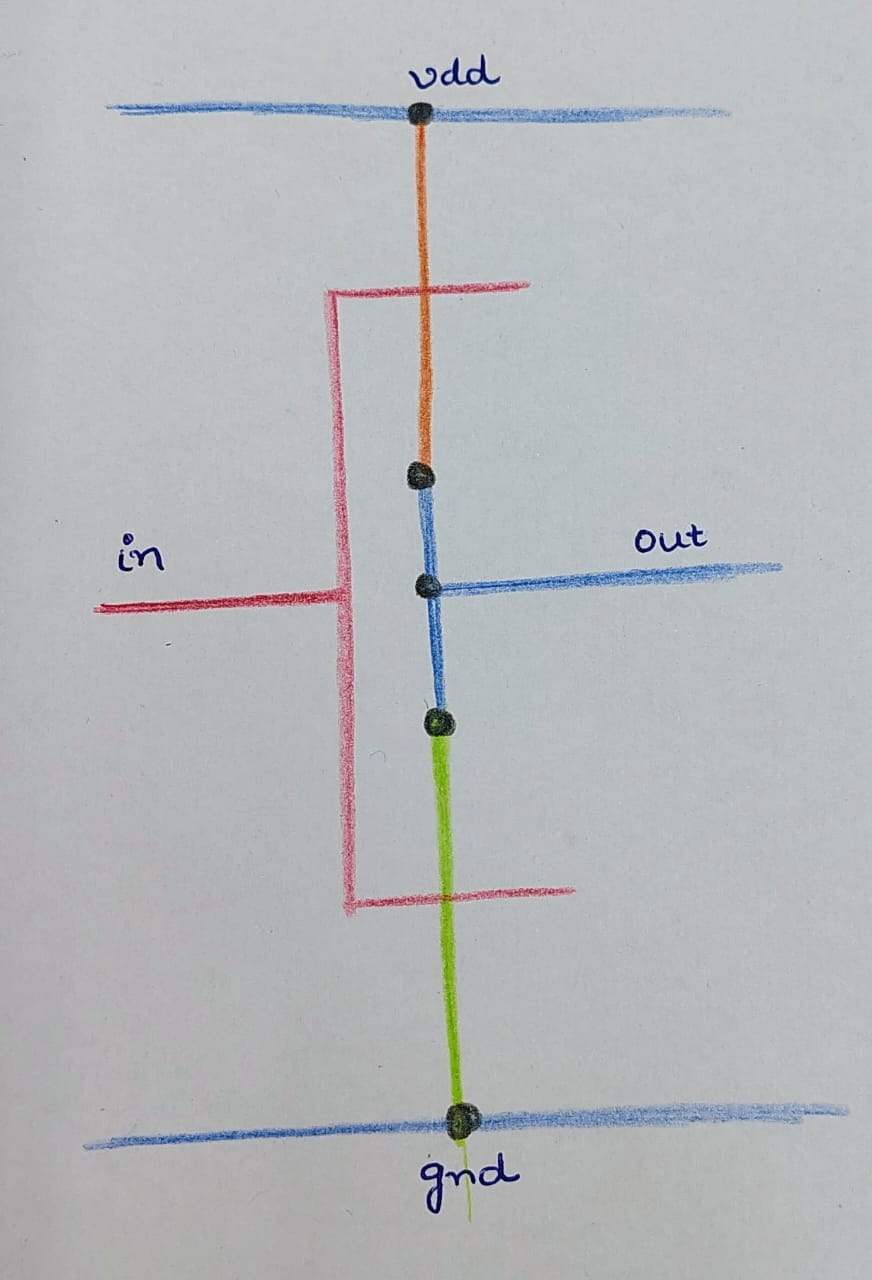
\includegraphics[width=1\linewidth]{stick_inv.jpg}
    \caption{Minimum Size Inverter}
    \label{fig:enter-label}
\end{figure}

\section{Block Wise Layout}
Layout of each block was designed using MAGIC layout editor and previously given technology file. Post layout parasitics are extracted, simulated and compared with the results from schematic simulation.\newline
As explained in section III about Layout Design Strategy, euler path method was used to construct Stick Diagrams and these have been used to make MAGIC Layout for each Block.
\begin{figure}[H]
    \centering
    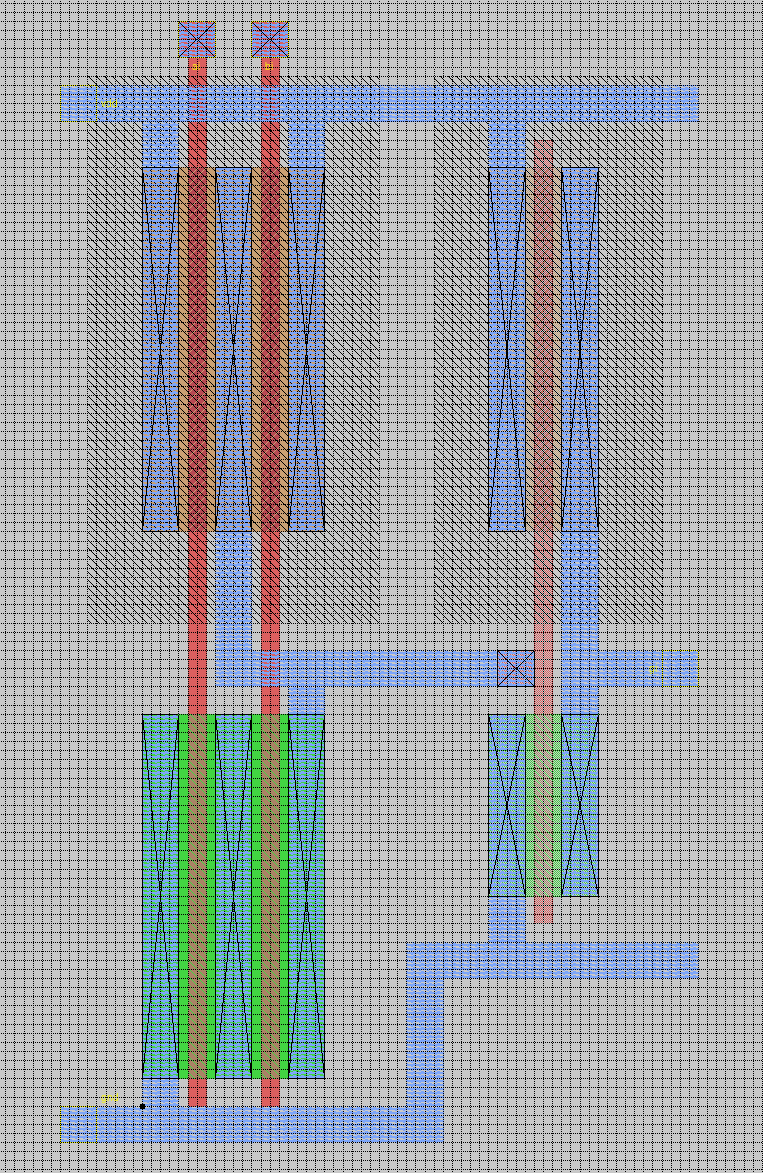
\includegraphics[width=1\linewidth]{Block_and.png}
    \caption{AND Gate}
    \label{fig:enter-label}
\end{figure}
\begin{figure}[H]
    \centering
    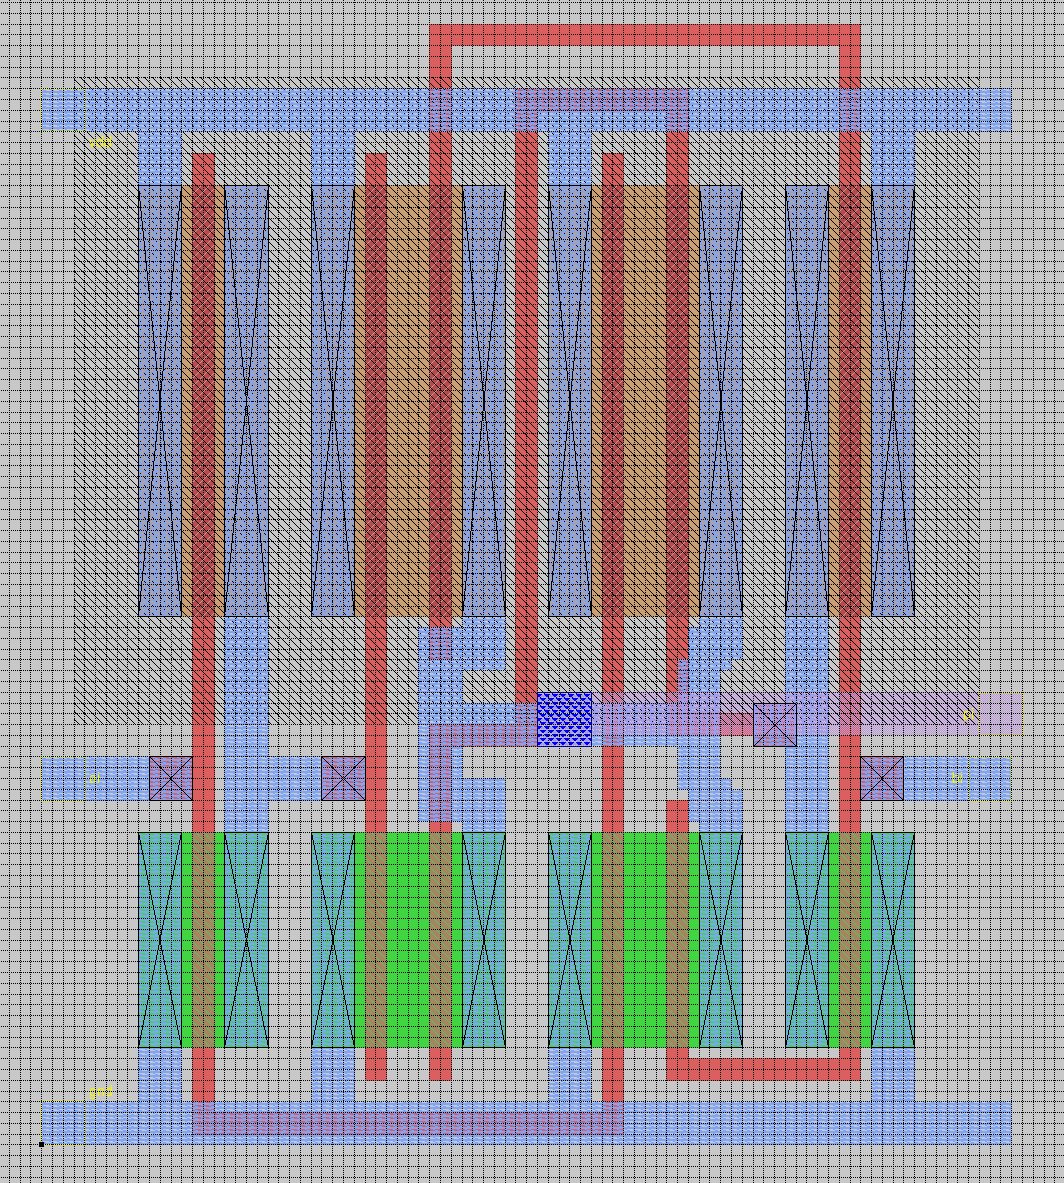
\includegraphics[width=0.9\linewidth]{Block_XOR.png}
    \caption{XOR Gate}
    \label{fig:enter-label}
\end{figure}
\begin{figure}[H]
    \centering
    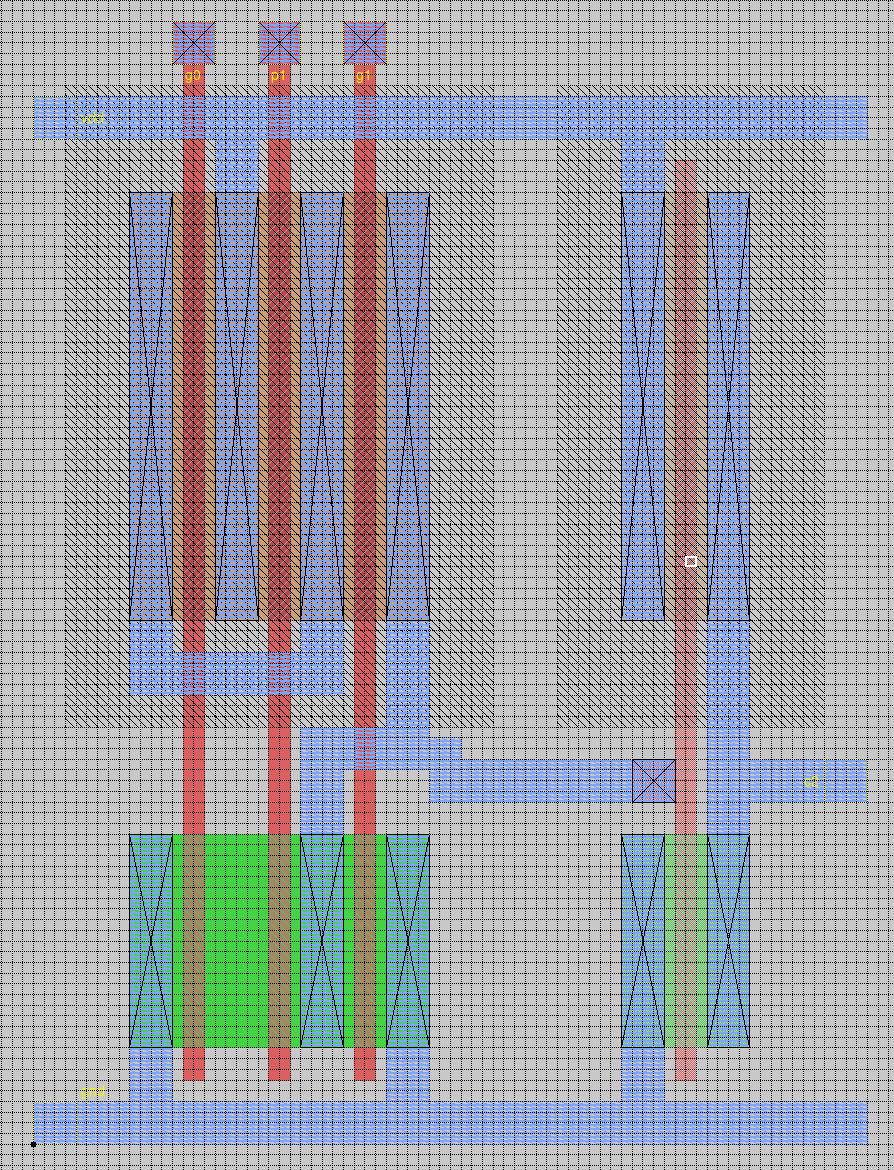
\includegraphics[width=0.9\linewidth]{Block_C2.png}
    \caption{C2 Logic}
    \label{fig:enter-label}
\end{figure}
\begin{figure}[H]
    \centering
    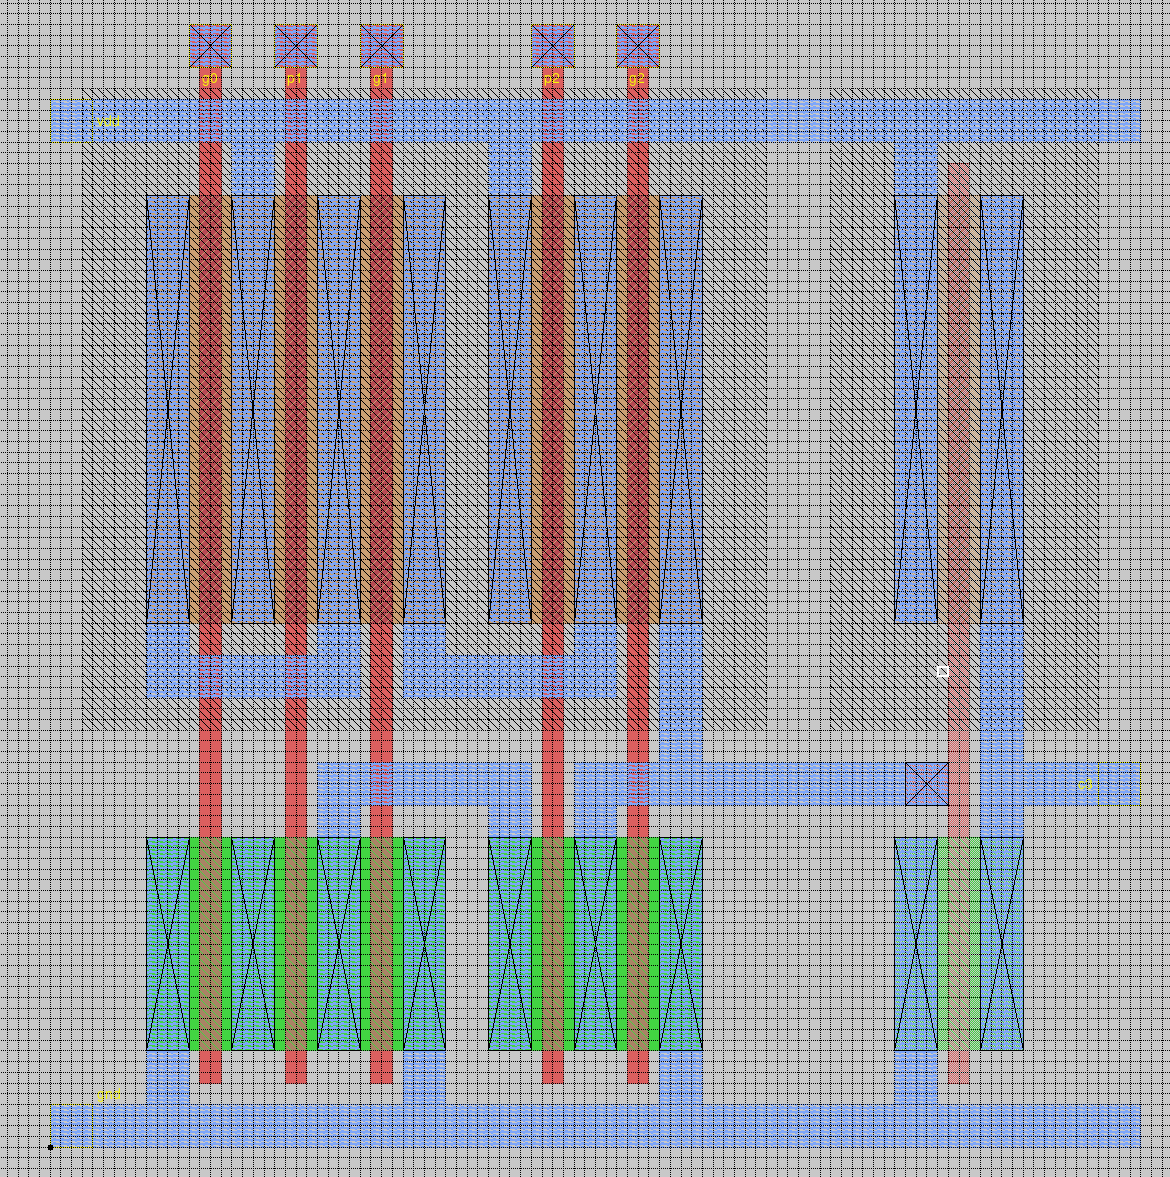
\includegraphics[width=1\linewidth]{Block_C3.png}
    \caption{C3 Logic}
    \label{fig:enter-label}
\end{figure}
\begin{figure}[H]
    \centering
    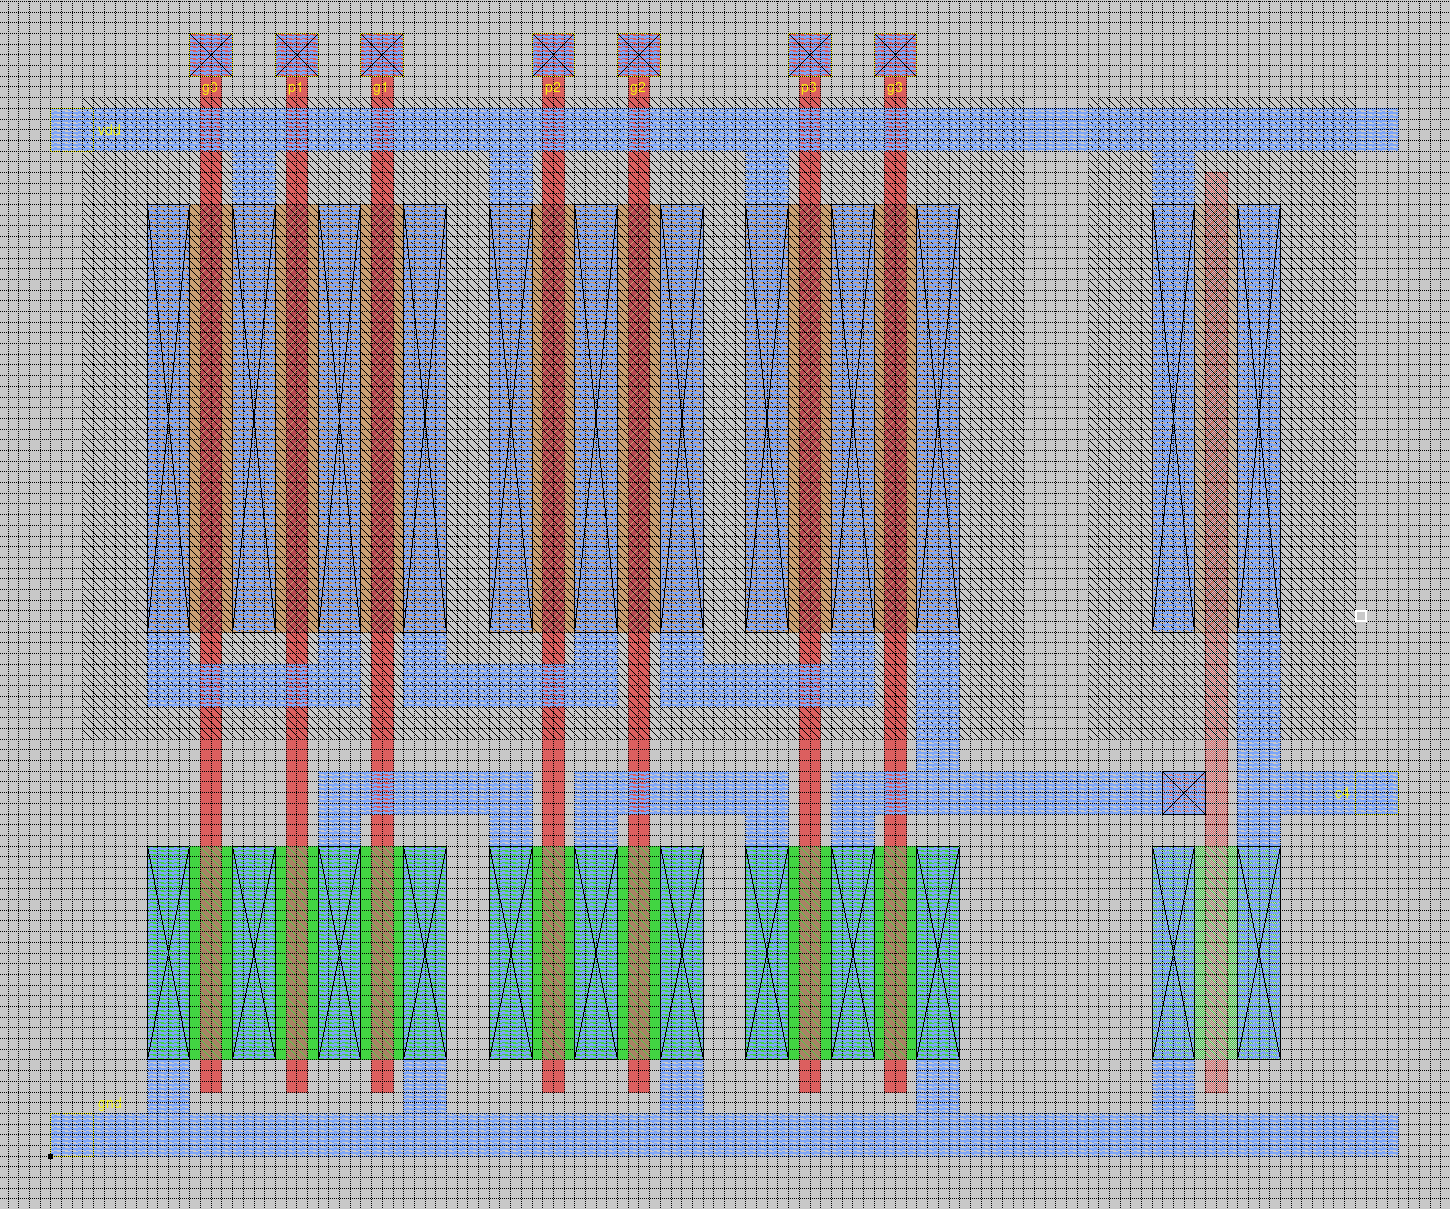
\includegraphics[width=1\linewidth]{Block_C4.png}
    \caption{C4 Logic}
    \label{fig:enter-label}
\end{figure}
\begin{figure}[H]
    \centering
    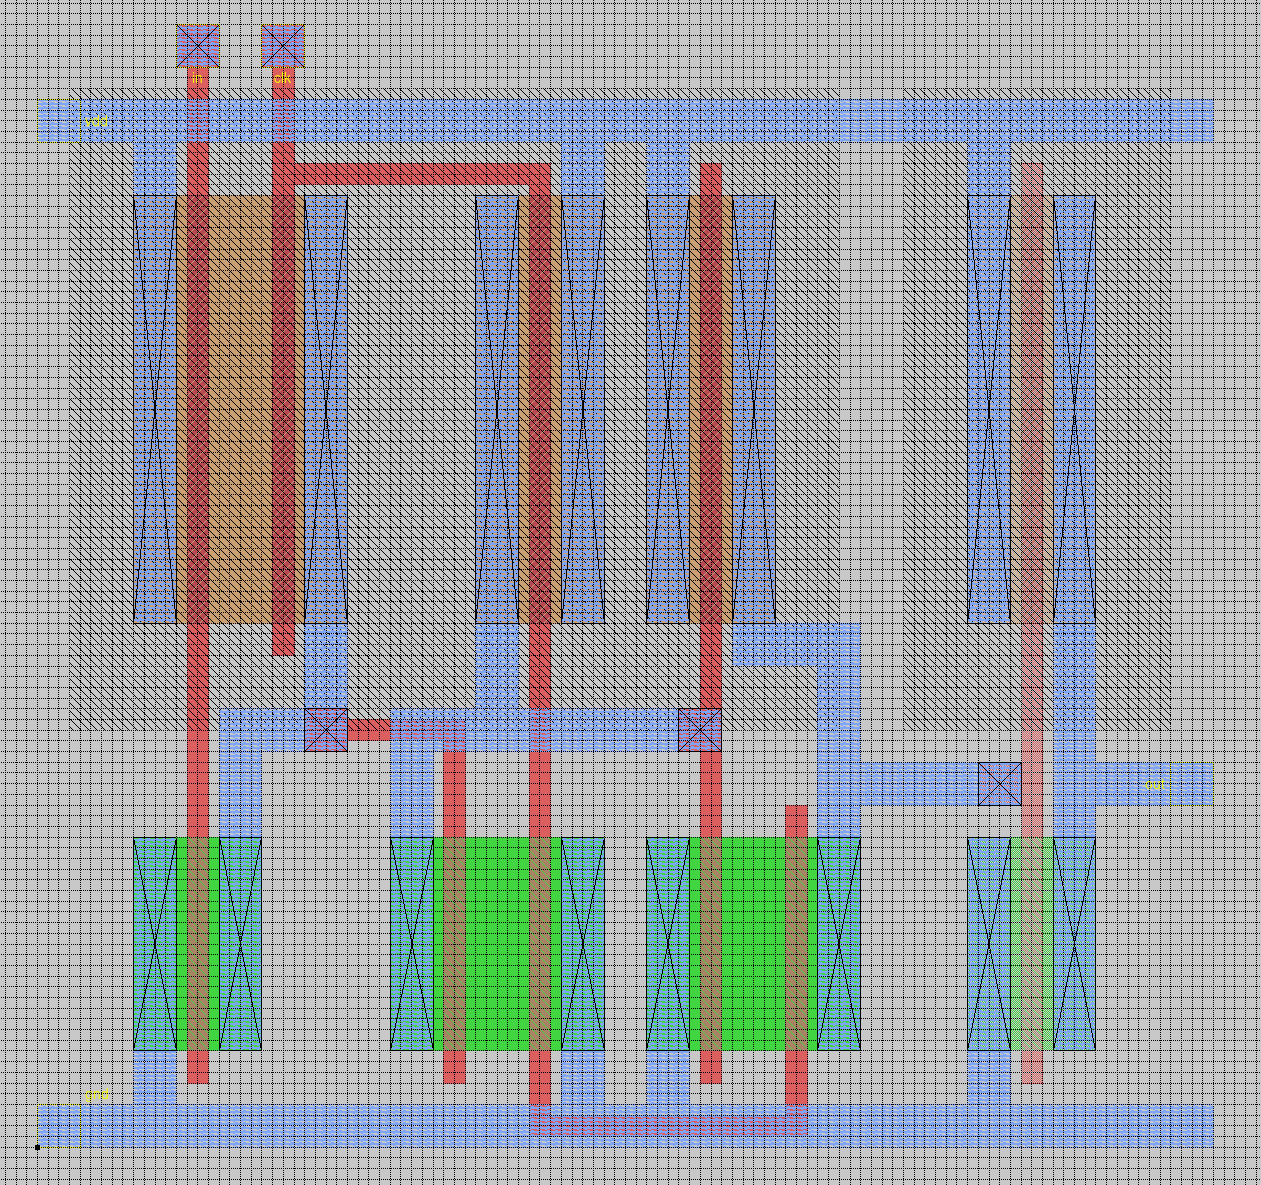
\includegraphics[width=1\linewidth]{Block_DFF.png}
    \caption{D Flip Flop}
    \label{fig:enter-label}
\end{figure}
\begin{figure}[H]
    \centering
    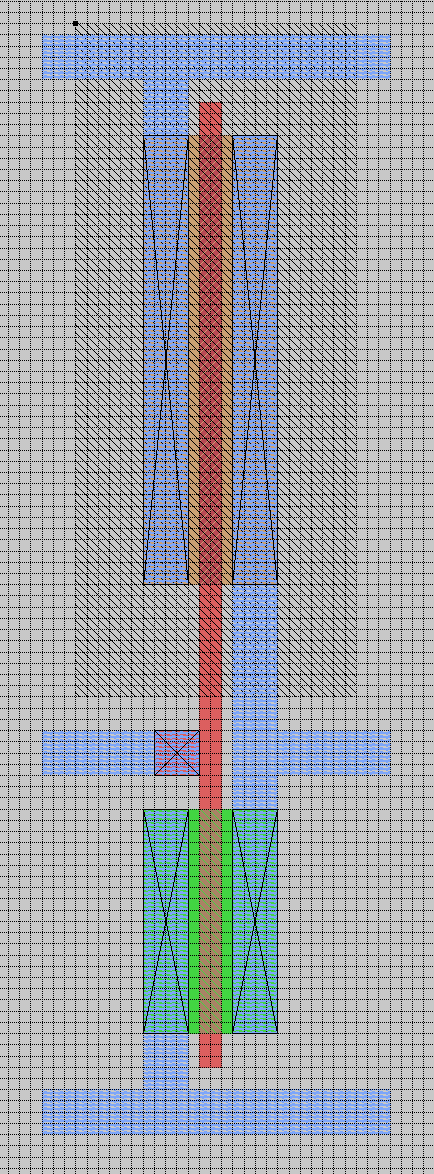
\includegraphics[width=0.5\linewidth]{Block_inv.png}
    \caption{Minimum Size Inverter (Used as subcell in other Layouts)}
    \label{fig:enter-label}
\end{figure}
As we can notice the circuit which could be constructed in single diffusion area is separated to decrease rise/fall times by increasing the amount of contacts to vdd and gnd thereby reducing resistance.\newline
\begin{figure}[H]
    \centering
    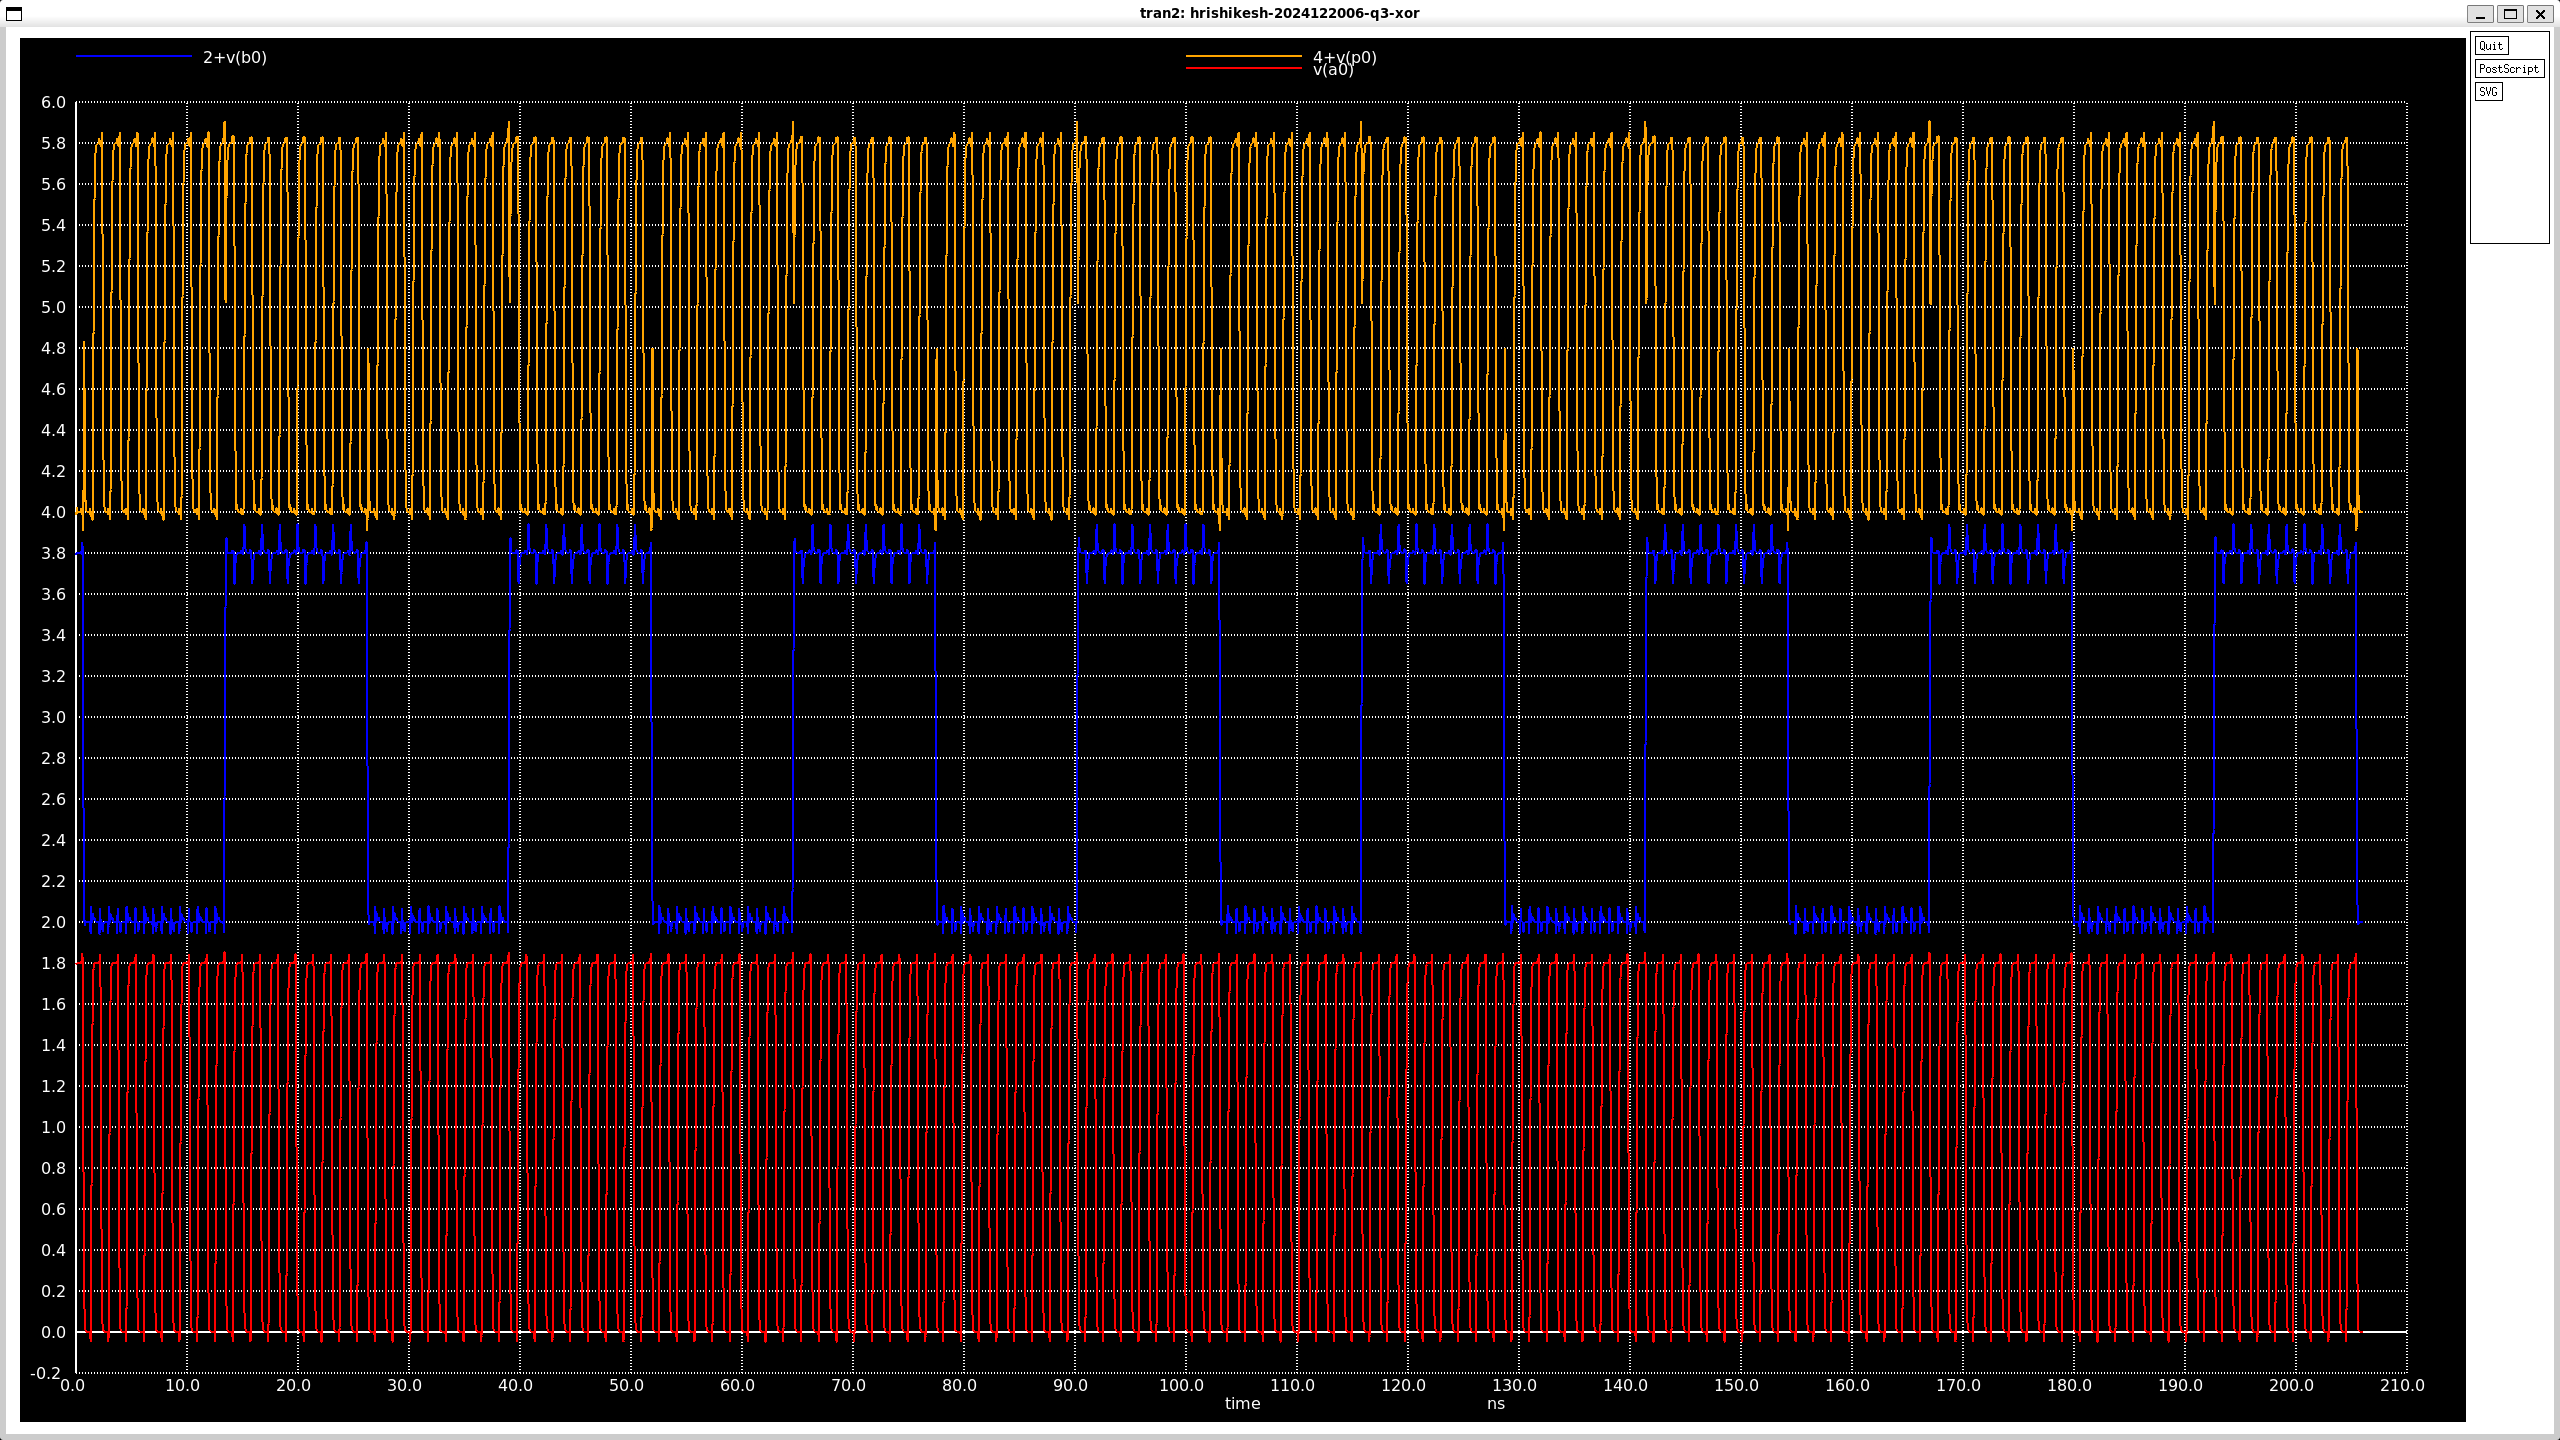
\includegraphics[width=1\linewidth]{module_xor.png}
    \caption{XOR Gate}
    \label{fig:enter-label}
\end{figure}
\begin{figure}[H]
    \centering
    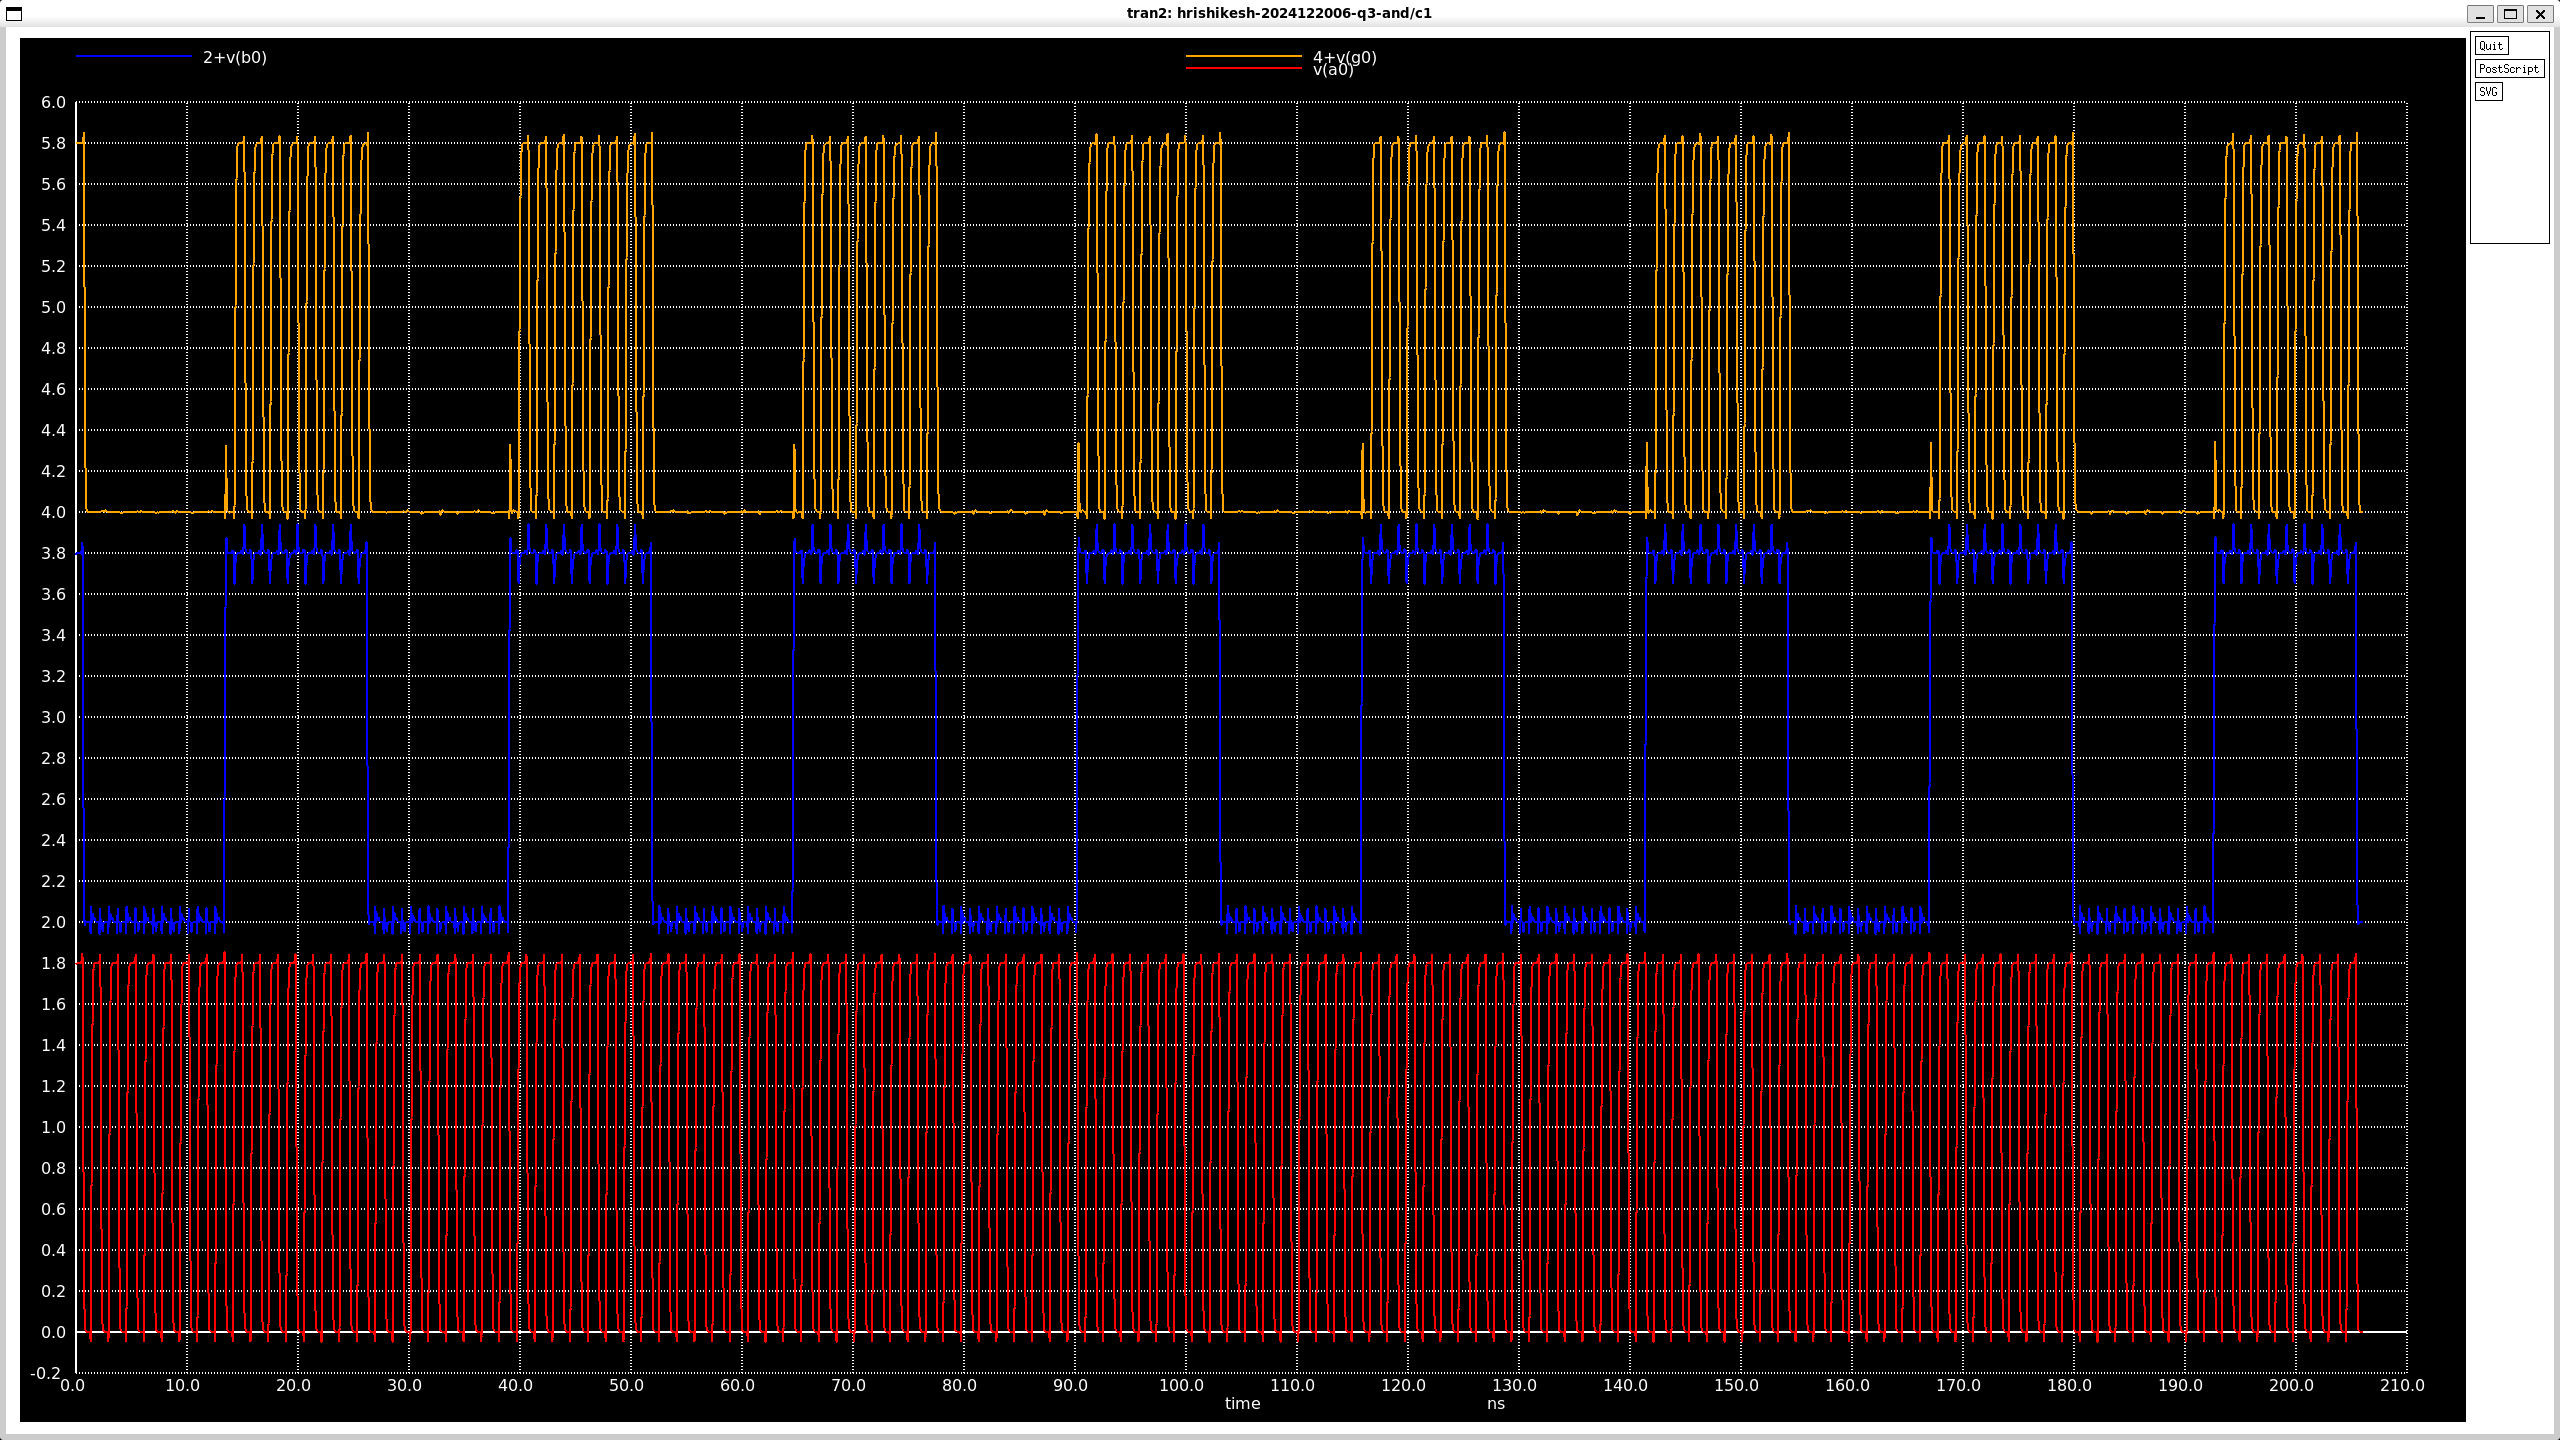
\includegraphics[width=1\linewidth]{module_and.png}
    \caption{AND Gate}
    \label{fig:enter-label}
\end{figure}
\begin{figure}[H]
    \centering
    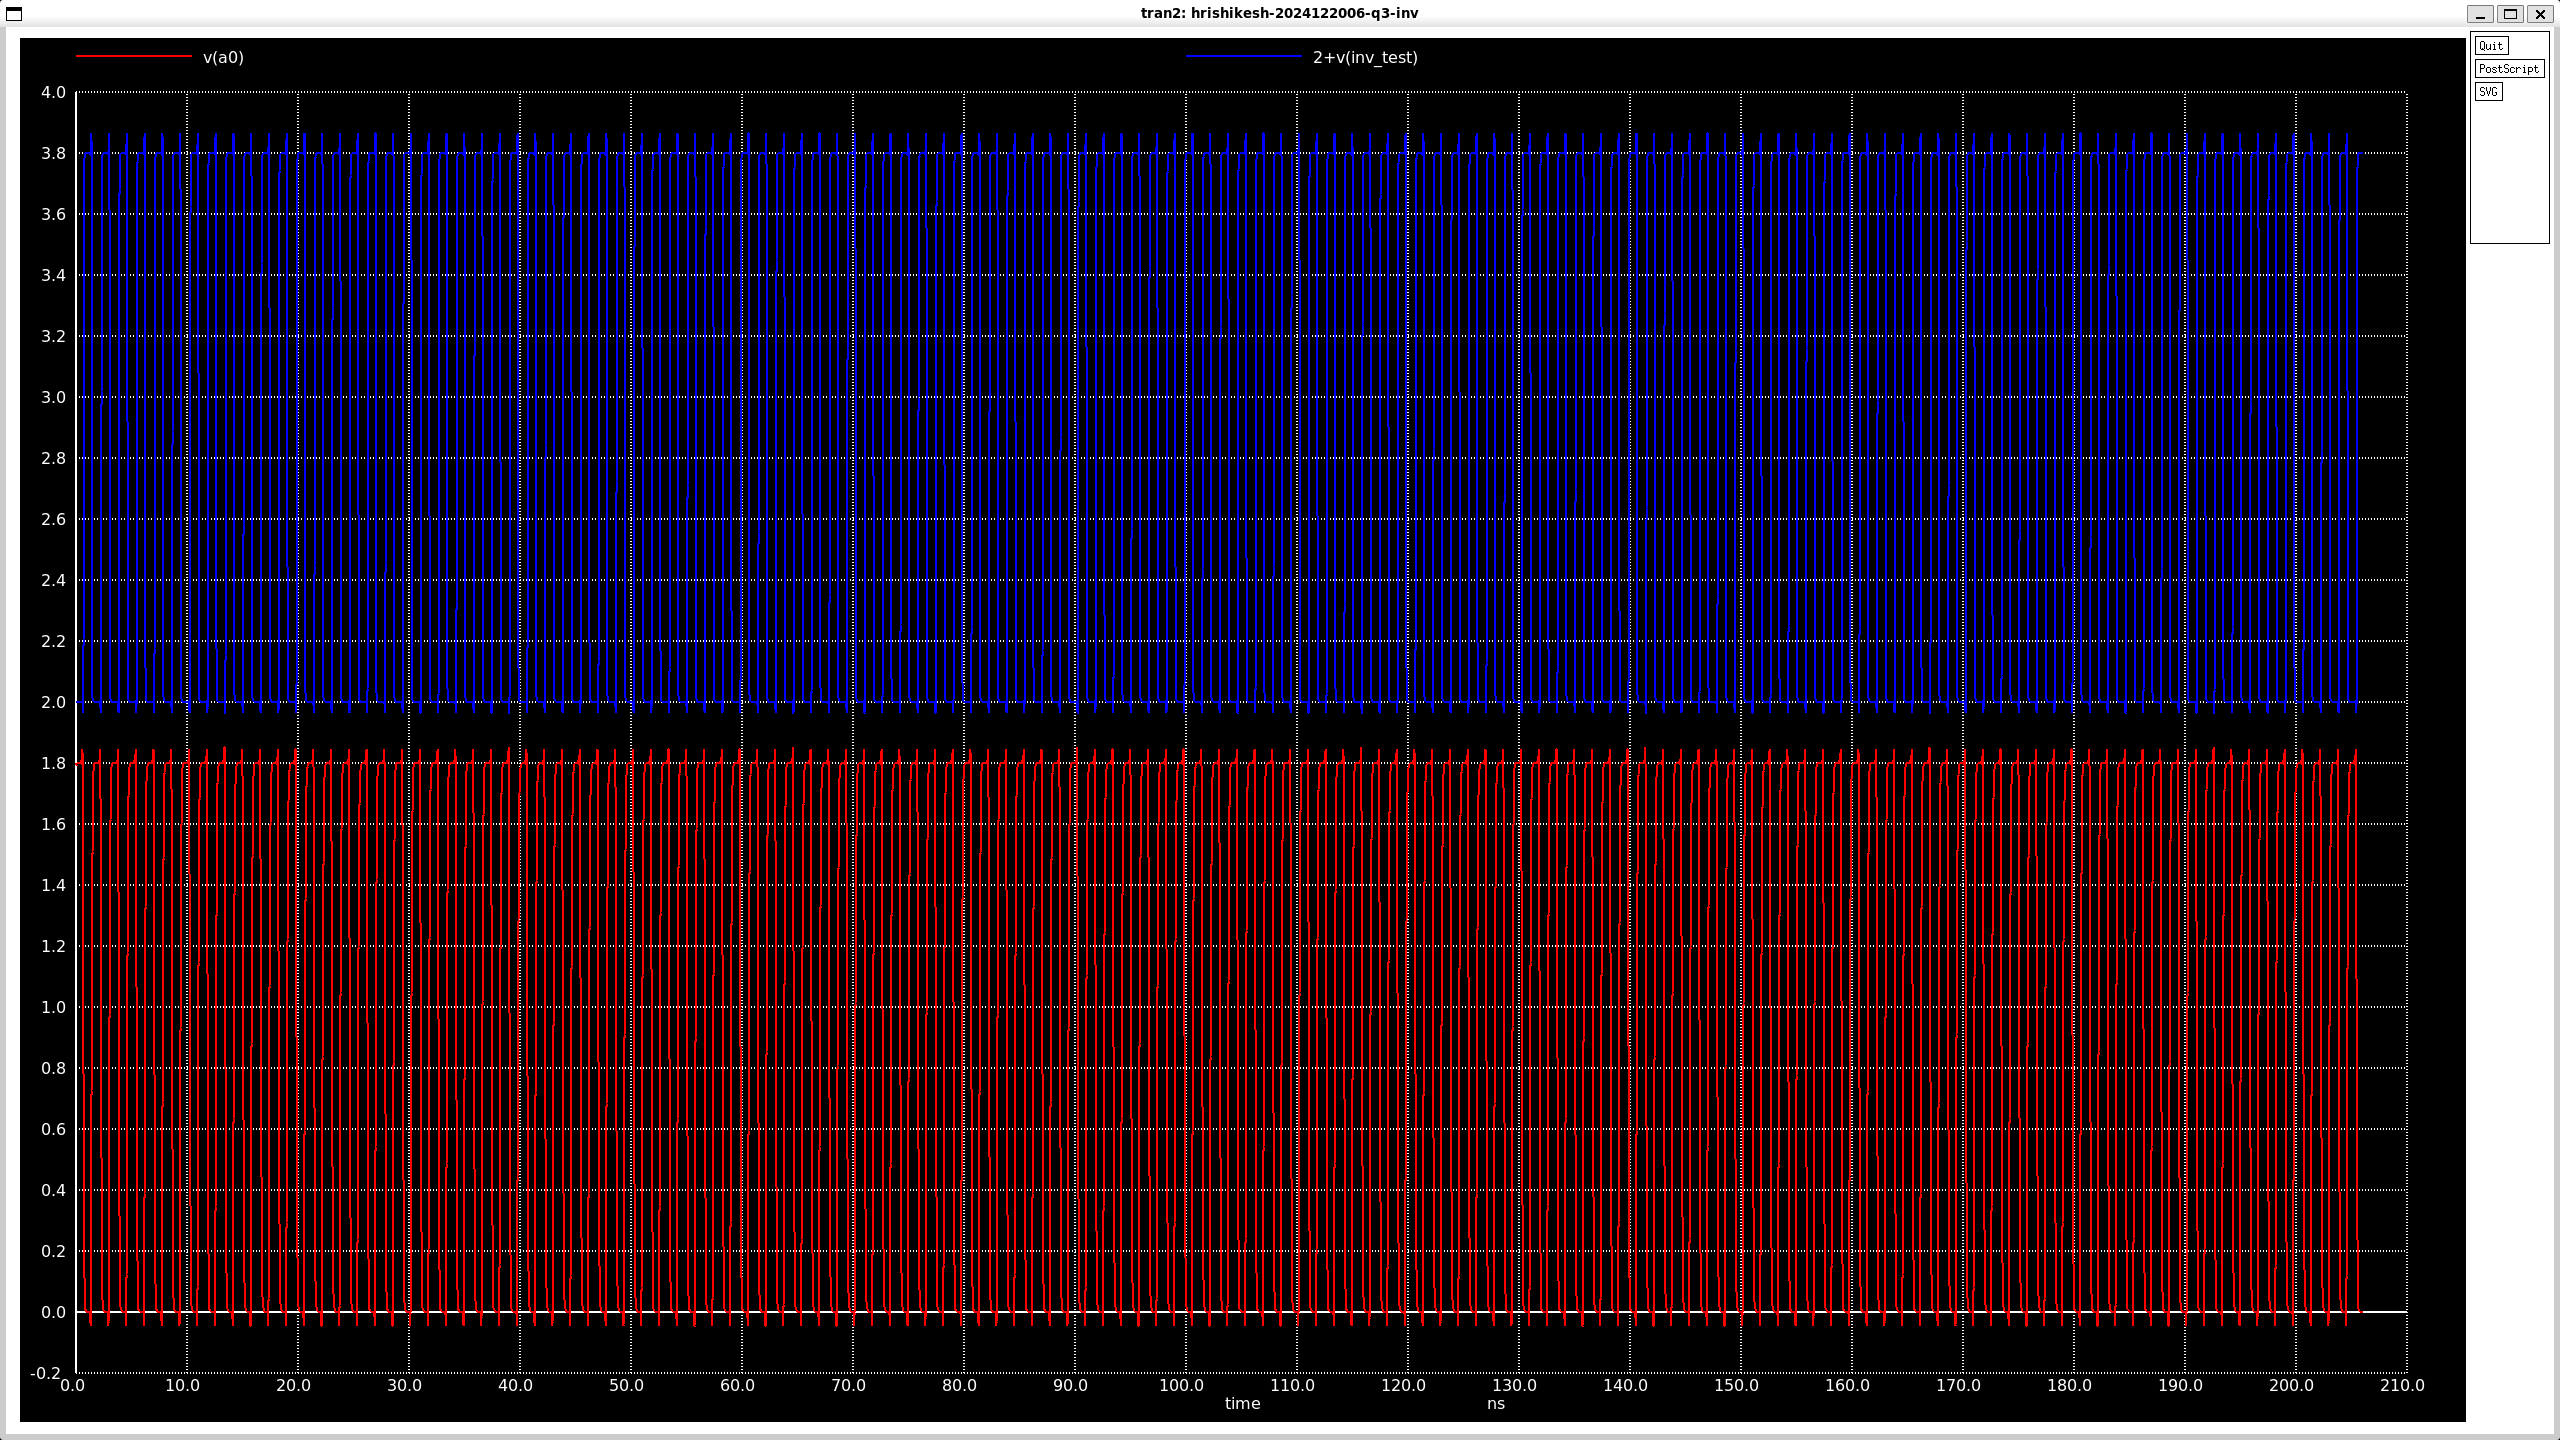
\includegraphics[width=1\linewidth]{module_inv.png}
    \caption{Inverter}
    \label{fig:enter-label}
\end{figure}
\begin{figure}[H]
    \centering
    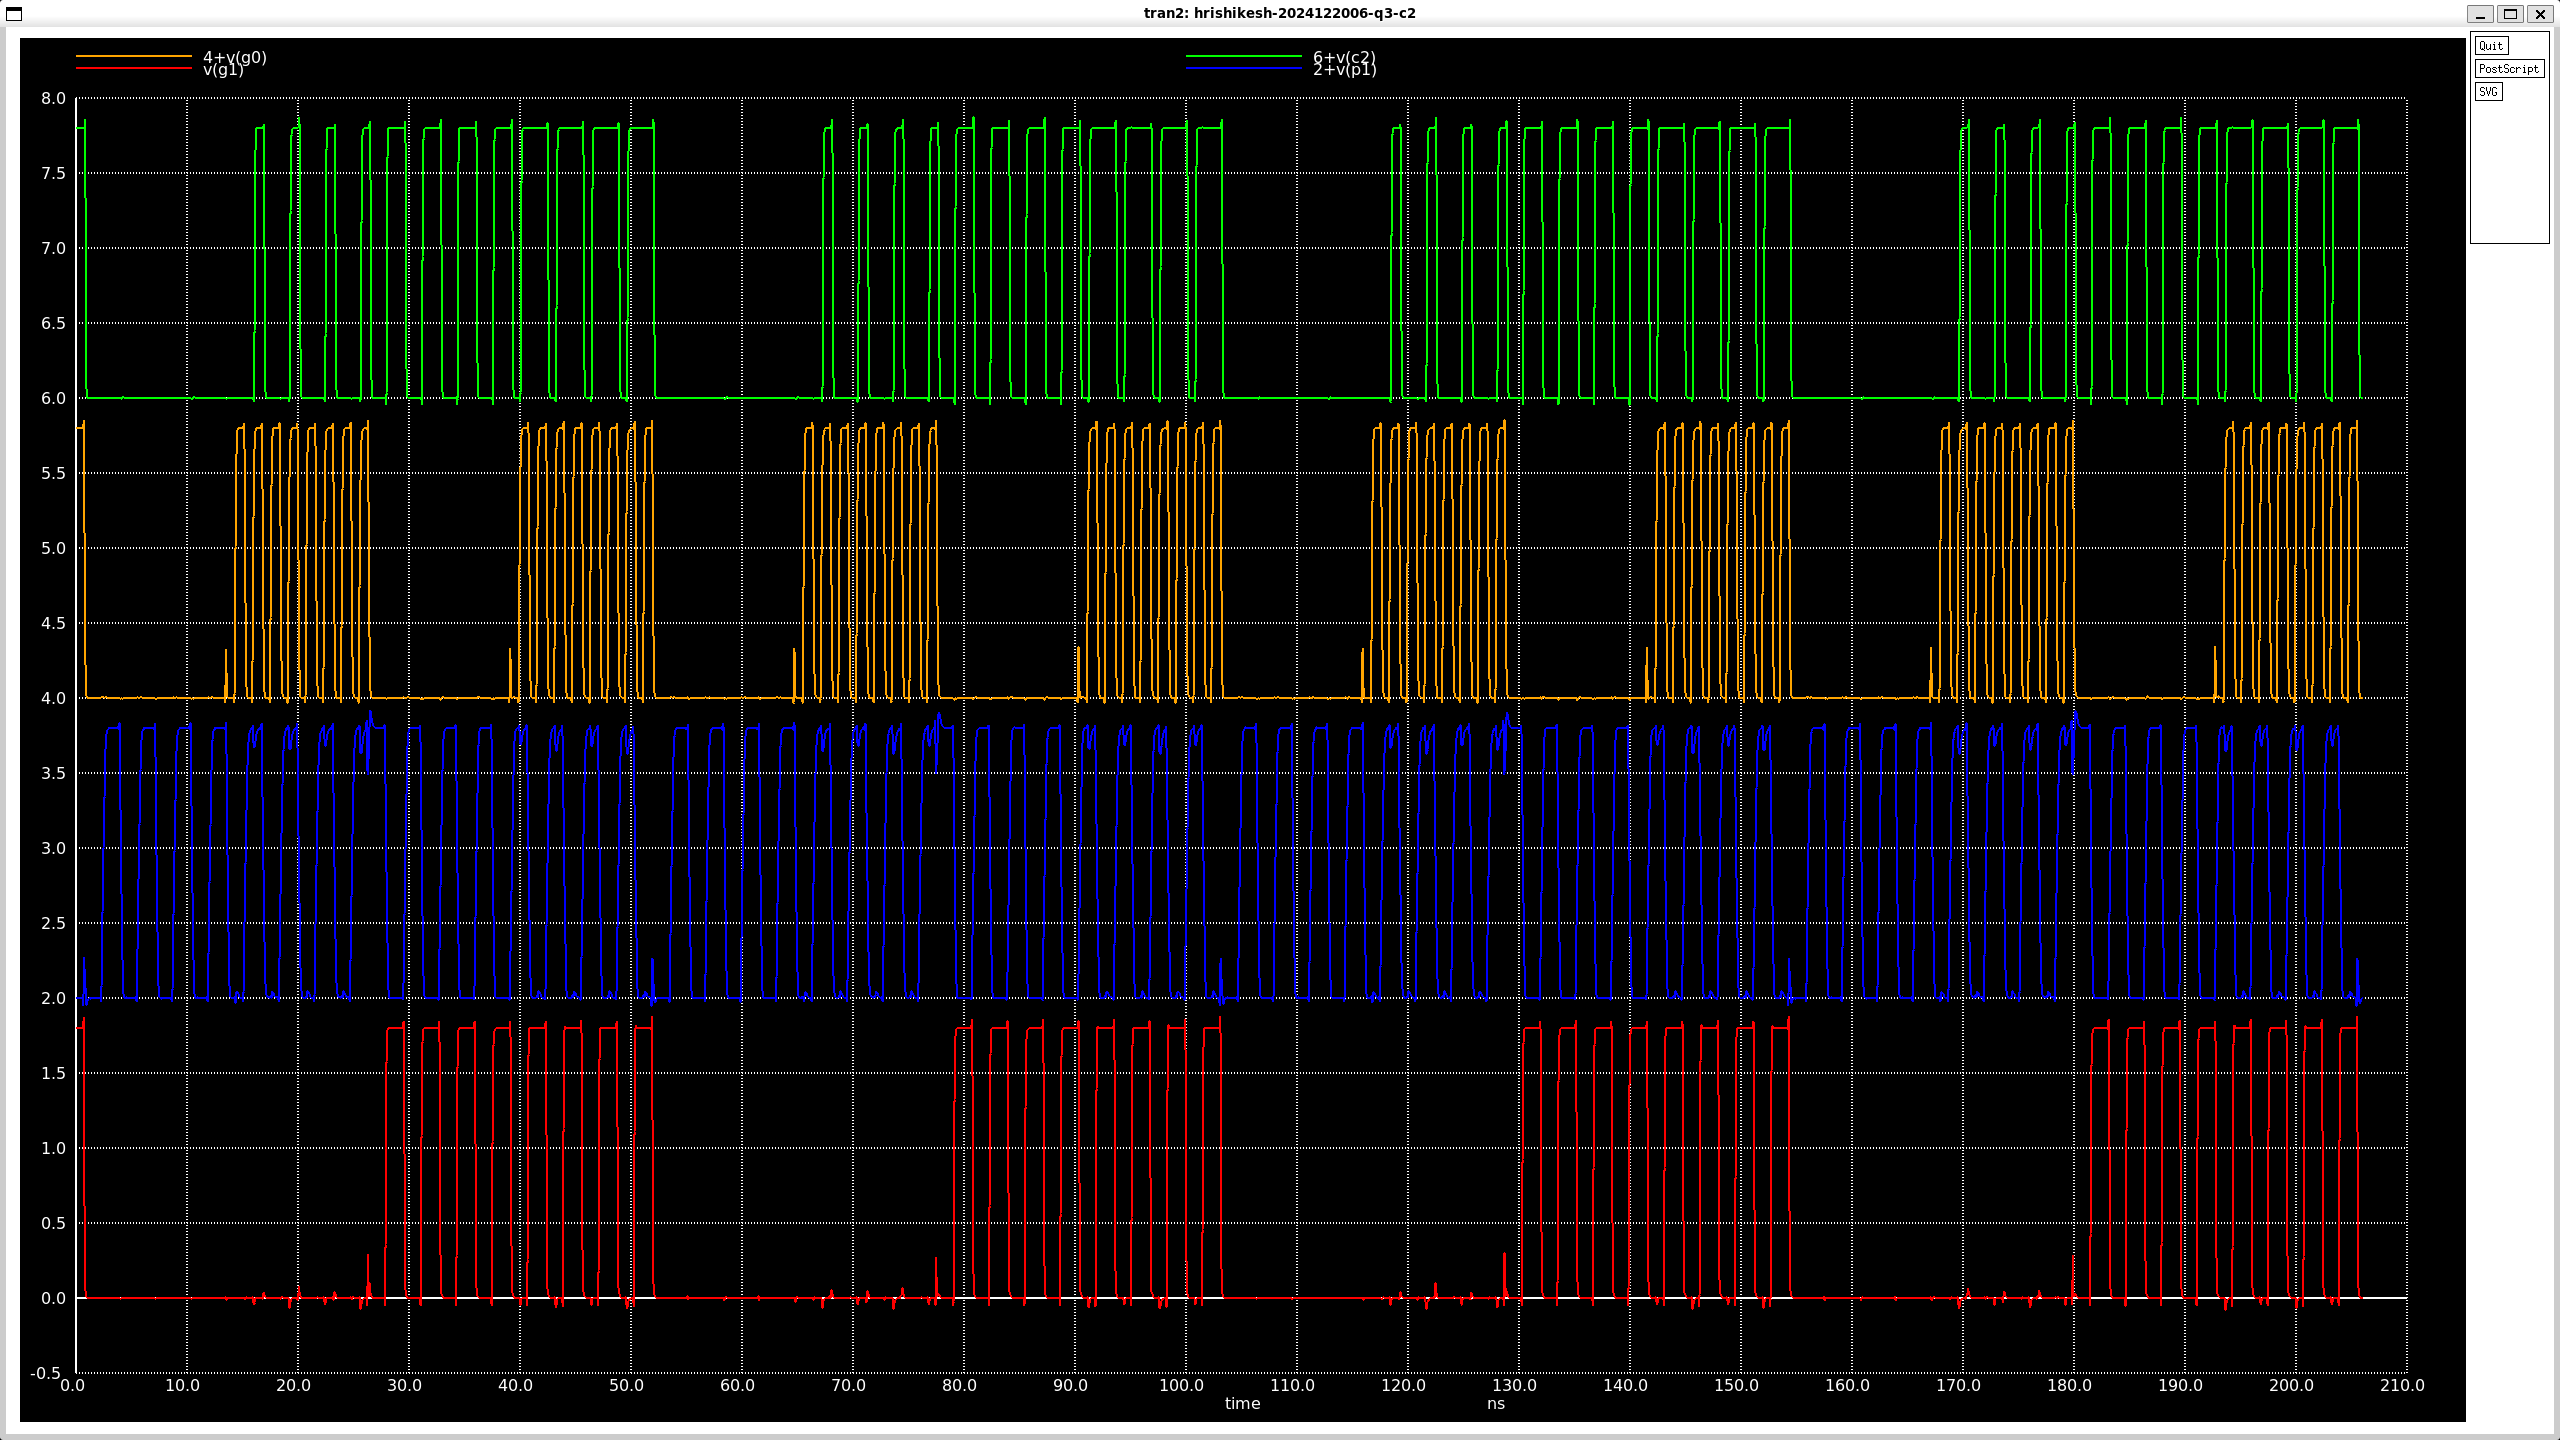
\includegraphics[width=1\linewidth]{C2 Logic.png}
    \caption{C2 Logic}
    \label{fig:enter-label}
\end{figure}
\begin{figure}[H]
    \centering
    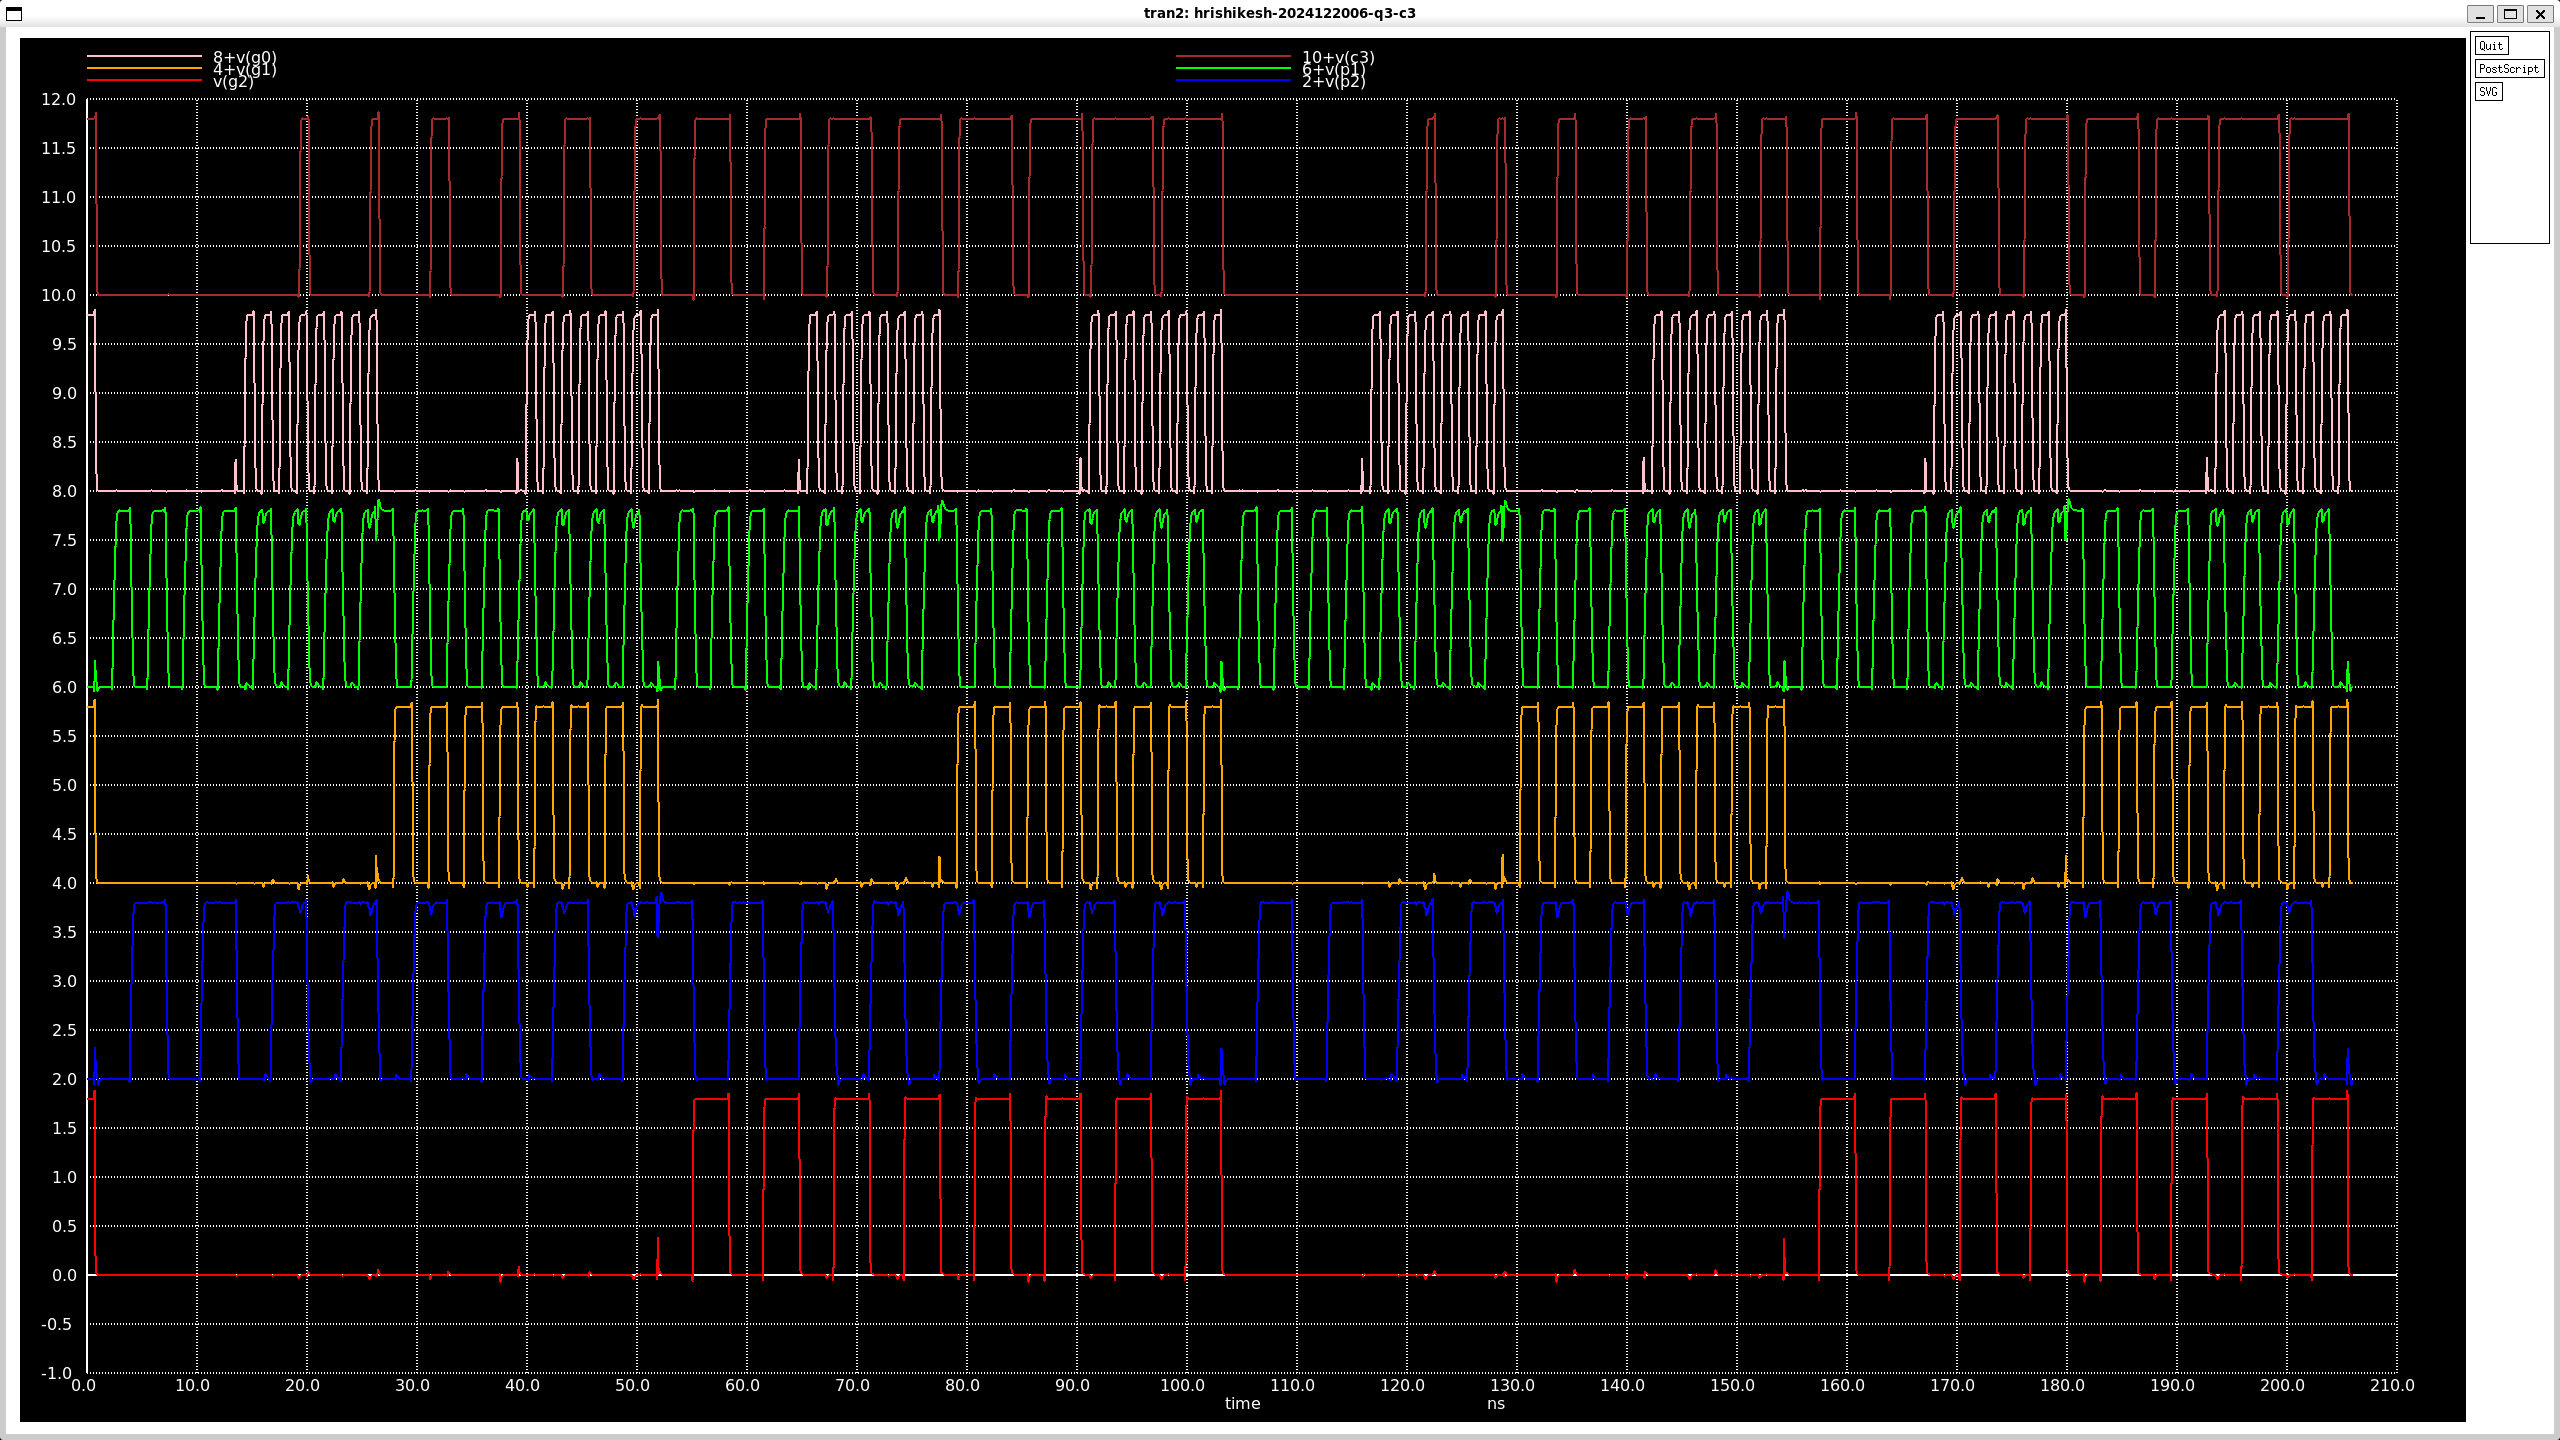
\includegraphics[width=1\linewidth]{module_c3.png}
    \caption{C3 Logic}
    \label{fig:enter-label}
\end{figure}
\begin{figure}[H]
    \centering
    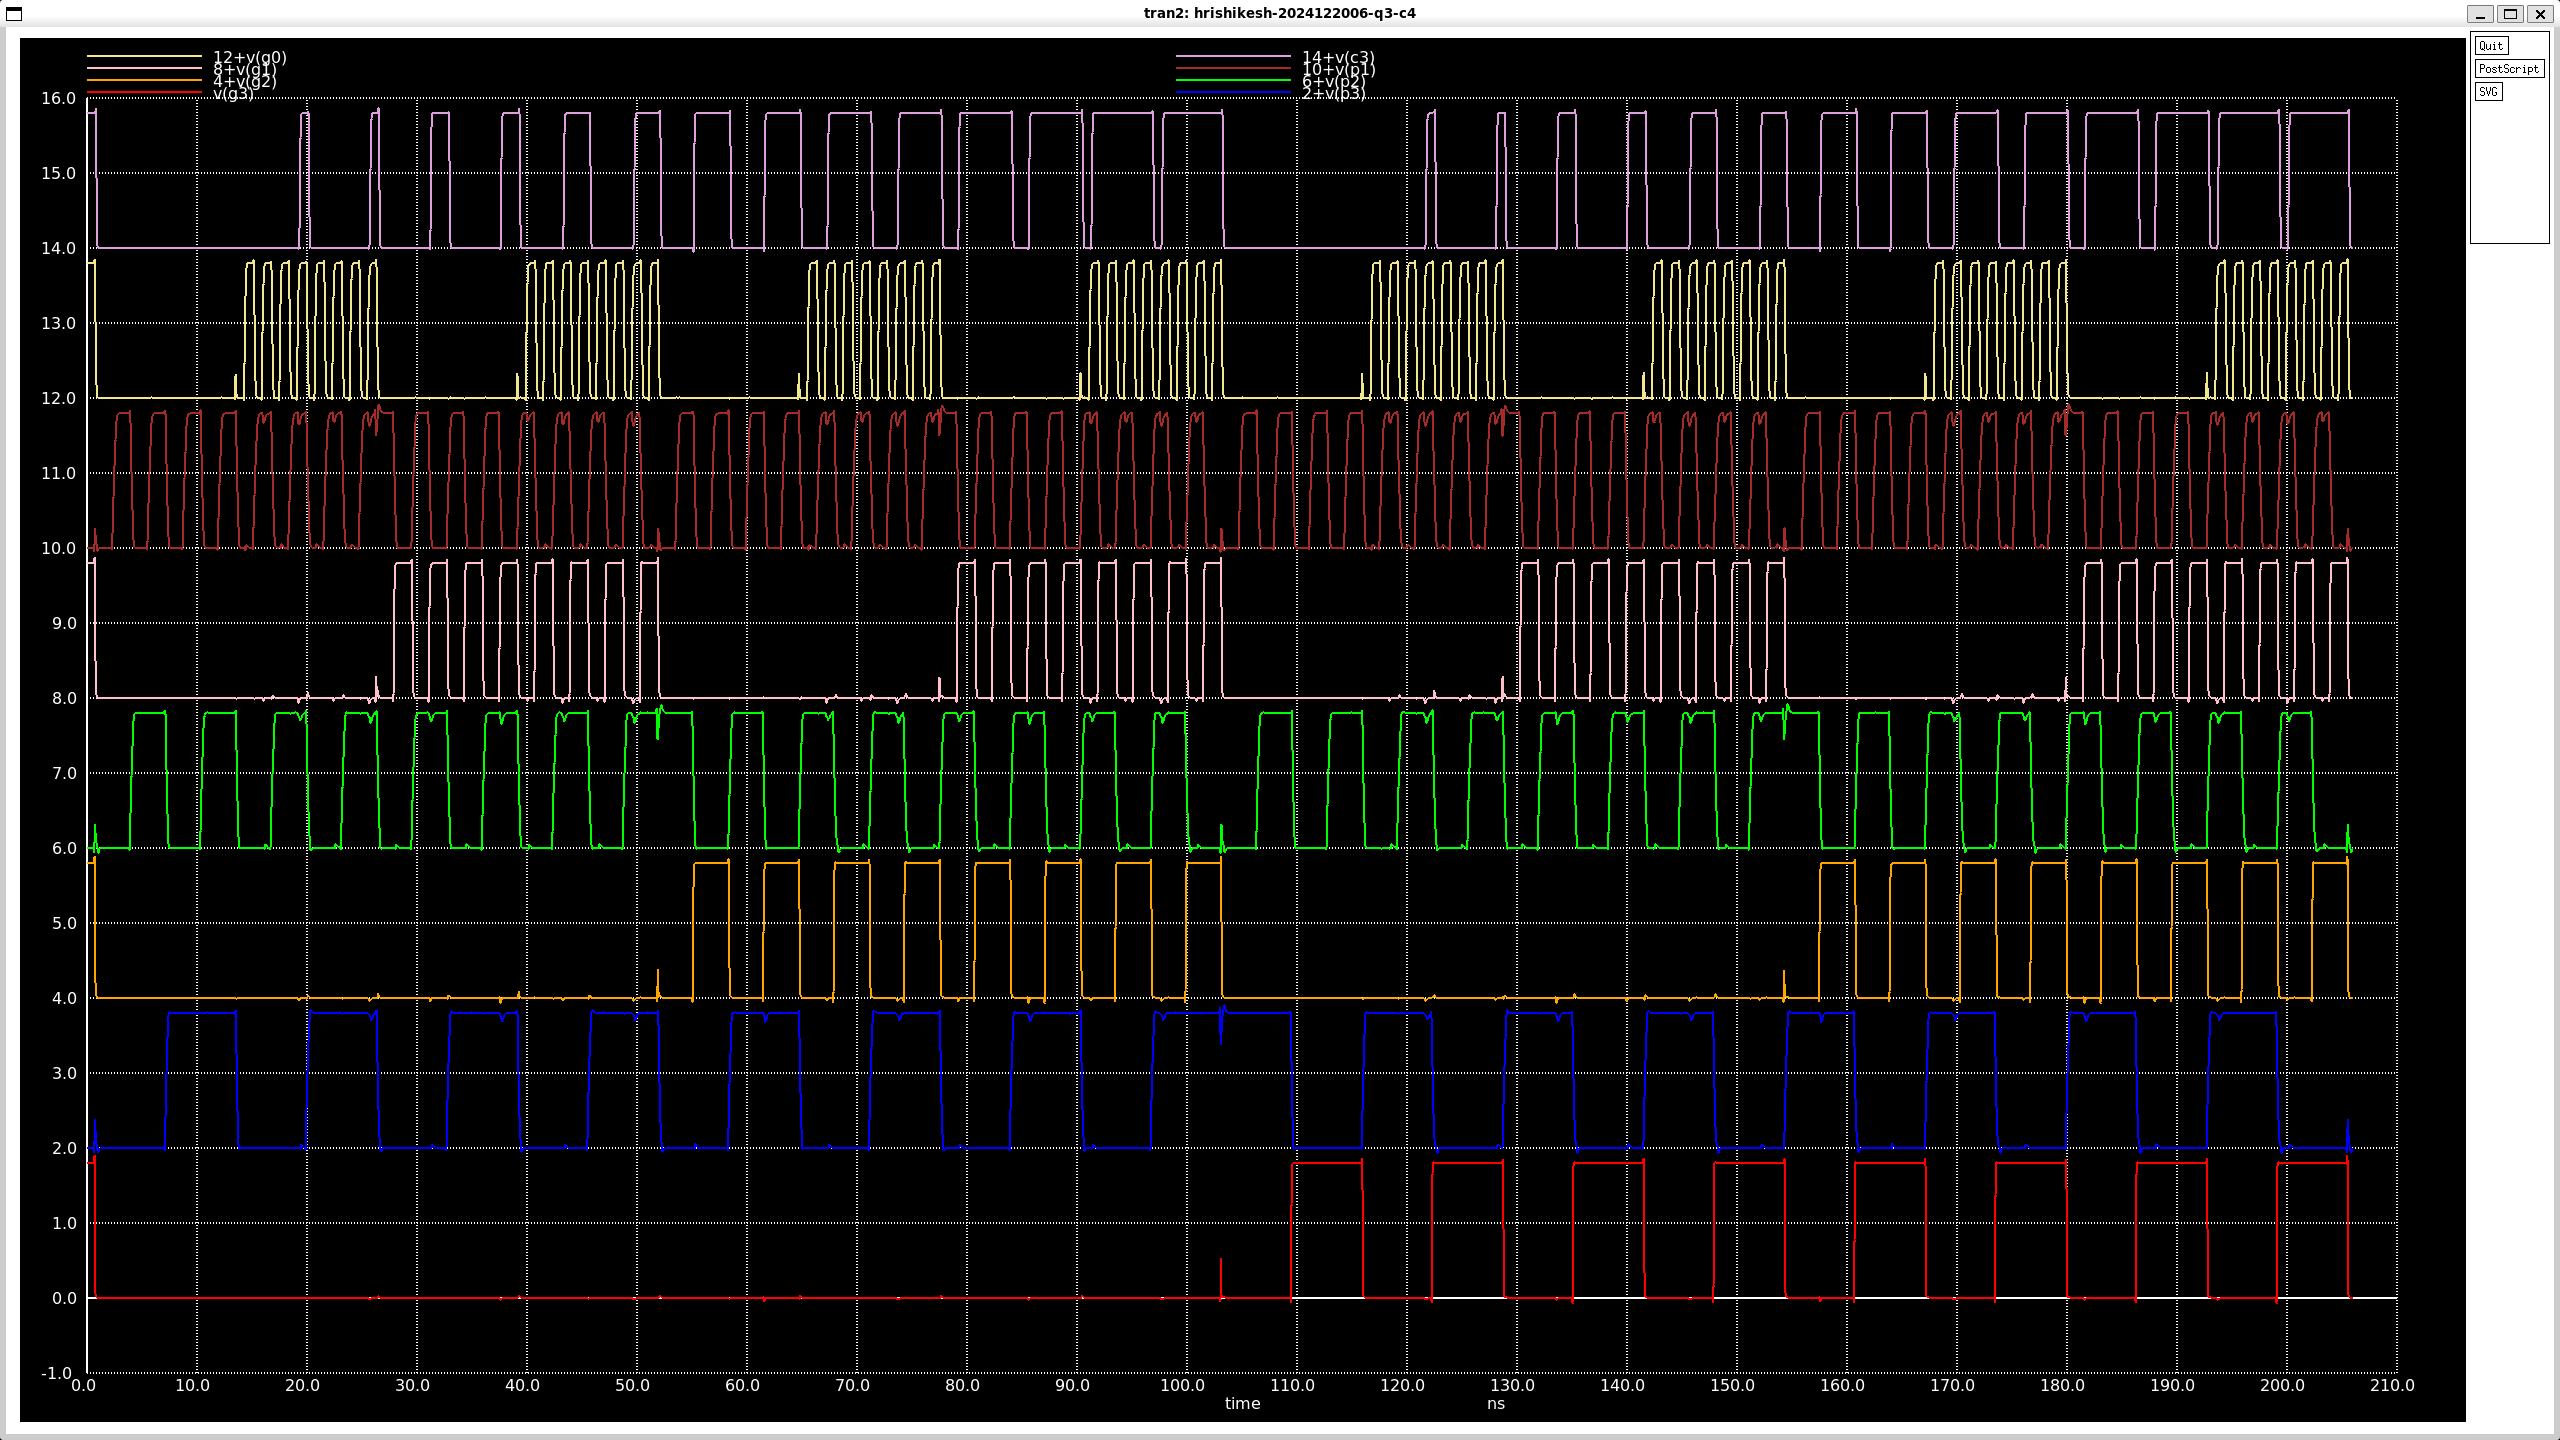
\includegraphics[width=1\linewidth]{module_c4.png}
    \caption{C4 Logic}
    \label{fig:enter-label}
\end{figure}
Results are compared with pre layout in Table I and II.

\begin{table*}[ht]
\centering
\caption{Comparison of Pre-Layout and Post-Layout Characteristics for Modules}
\begin{tabular}{|m{4cm}|m{3cm}|m{3cm}|m{3cm}|m{3cm}|}
\hline
\multirow{2}{*}{\textbf{Module}} & \multicolumn{2}{c|}{\textbf{Pre-Layout Characteristics}} & \multicolumn{2}{c|}{\textbf{Post-Layout Characteristics}} \\ \cline{2-5}
& \textbf{Delay (s)} & \textbf{RMS Power (W)} & \textbf{Delay (s)} & \textbf{RMS Power (W)} \\ 
\hline
Inverter & $5.30549 \times 10^{-11}$ & $2.08383 \times 10^{-4}$ & $5.34761 \times 10^{-11}$ & $2.13370 \times 10^{-4}$ \\ 
\hline
XOR Gate & $1.38618 \times 10^{-10}$ & $3.34009 \times 10^{-4}$ & $9.59316 \times 10^{-10}$ & $3.46414 \times 10^{-4}$ \\ 
\hline
AND Gate & $1.59971 \times 10^{-10}$ & $4.97616 \times 10^{-4}$ & $1.60520 \times 10^{-10}$ & $3.68890 \times 10^{-4}$ \\ 
\hline
$C_2$ Logic & $2.86838 \times 10^{-10}$ & $2.43924 \times 10^{-4}$ & $2.89997 \times 10^{-10}$ & $2.22642 \times 10^{-4}$ \\ 
\hline
$C_3$ Logic & $3.89675 \times 10^{-10}$ & $1.90786 \times 10^{-4}$ & $3.63056 \times 10^{-10}$ & $1.82896 \times 10^{-4}$ \\ 
\hline
$C_4$ Logic & $4.97499 \times 10^{-10}$ & $1.47645 \times 10^{-4}$ & $4.52454 \times 10^{-10}$ & $1.41928 \times 10^{-4}$ \\ 
\hline
\end{tabular}
\label{tab:module_comparison}
\end{table*}

% DFF Comparison Table
\begin{table*}[ht]
\centering
\caption{Comparison of Pre-Layout and Post-Layout Characteristics for DFF}
\begin{tabular}{|c|c|c|c|c|c|c|}
\hline
\multirow{2}{*}{\textbf{Transition}} & \multicolumn{3}{c|}{\textbf{Pre-Layout Characteristics}} & \multicolumn{3}{c|}{\textbf{Post-Layout Characteristics}} \\ \cline{2-7}
& \boldmath$t_{\text{setup}}$ & \boldmath$t_{\text{hold}}$ & \boldmath$t_p$ & \boldmath$t_{\text{setup}}$ & \boldmath$t_{\text{hold}}$ & \boldmath$t_p$ \\ \hline
Low to High & 24 ps * & 40 ps * & $8.953852 \times 10^{-11}$ & 24 ps * & 20 ps * & $9.642945 \times 10^{-11}$ \\ \hline
High to Low & 50 ps & 30 ps & $1.466006 \times 10^{-10}$ & 24 ps & 33 ps & $1.468210 \times 10^{-10}$ \\ \hline
Final & 50 ps & 30 ps & $1.18070 \times 10^{-10}$ & 24 ps & 33 ps & $1.21625 \times 10^{-10}$ \\ \hline
\end{tabular}
\label{tab:dff_comparison}
\end{table*}


\section{Final Netlist}
Different blocks designed in previous steps are integrated and a netlist is written for the full circuit shown below.
\begin{figure}[H]
    \centering
    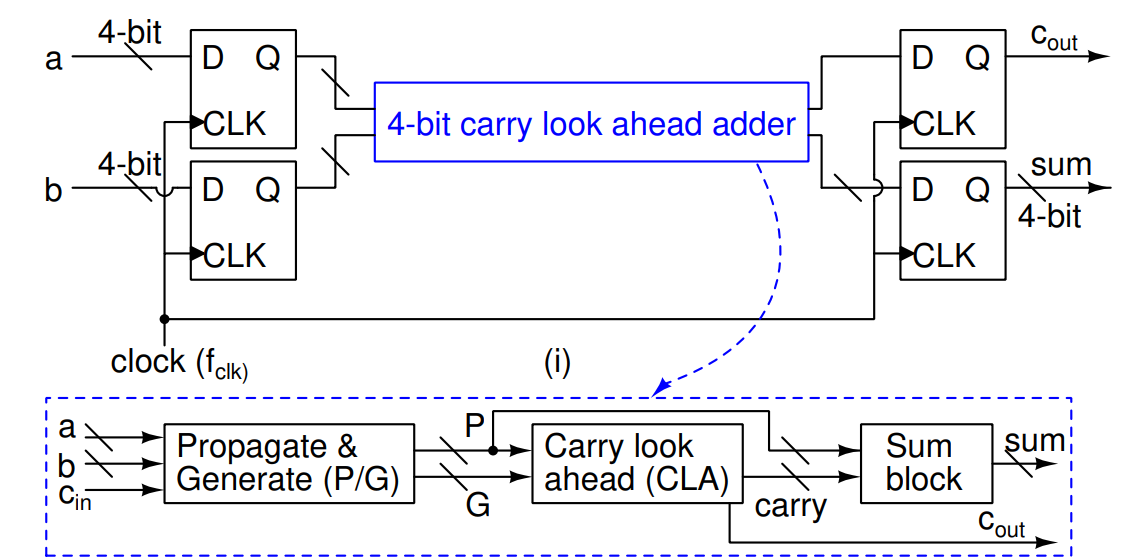
\includegraphics[width=1\linewidth]{Full_schematic.png}
    \caption{Full Schematic}
    \label{fig:enter-label}
\end{figure}
Using NGSPICE the functionality of the circuit is verified.
\begin{figure}[H]
    \centering
    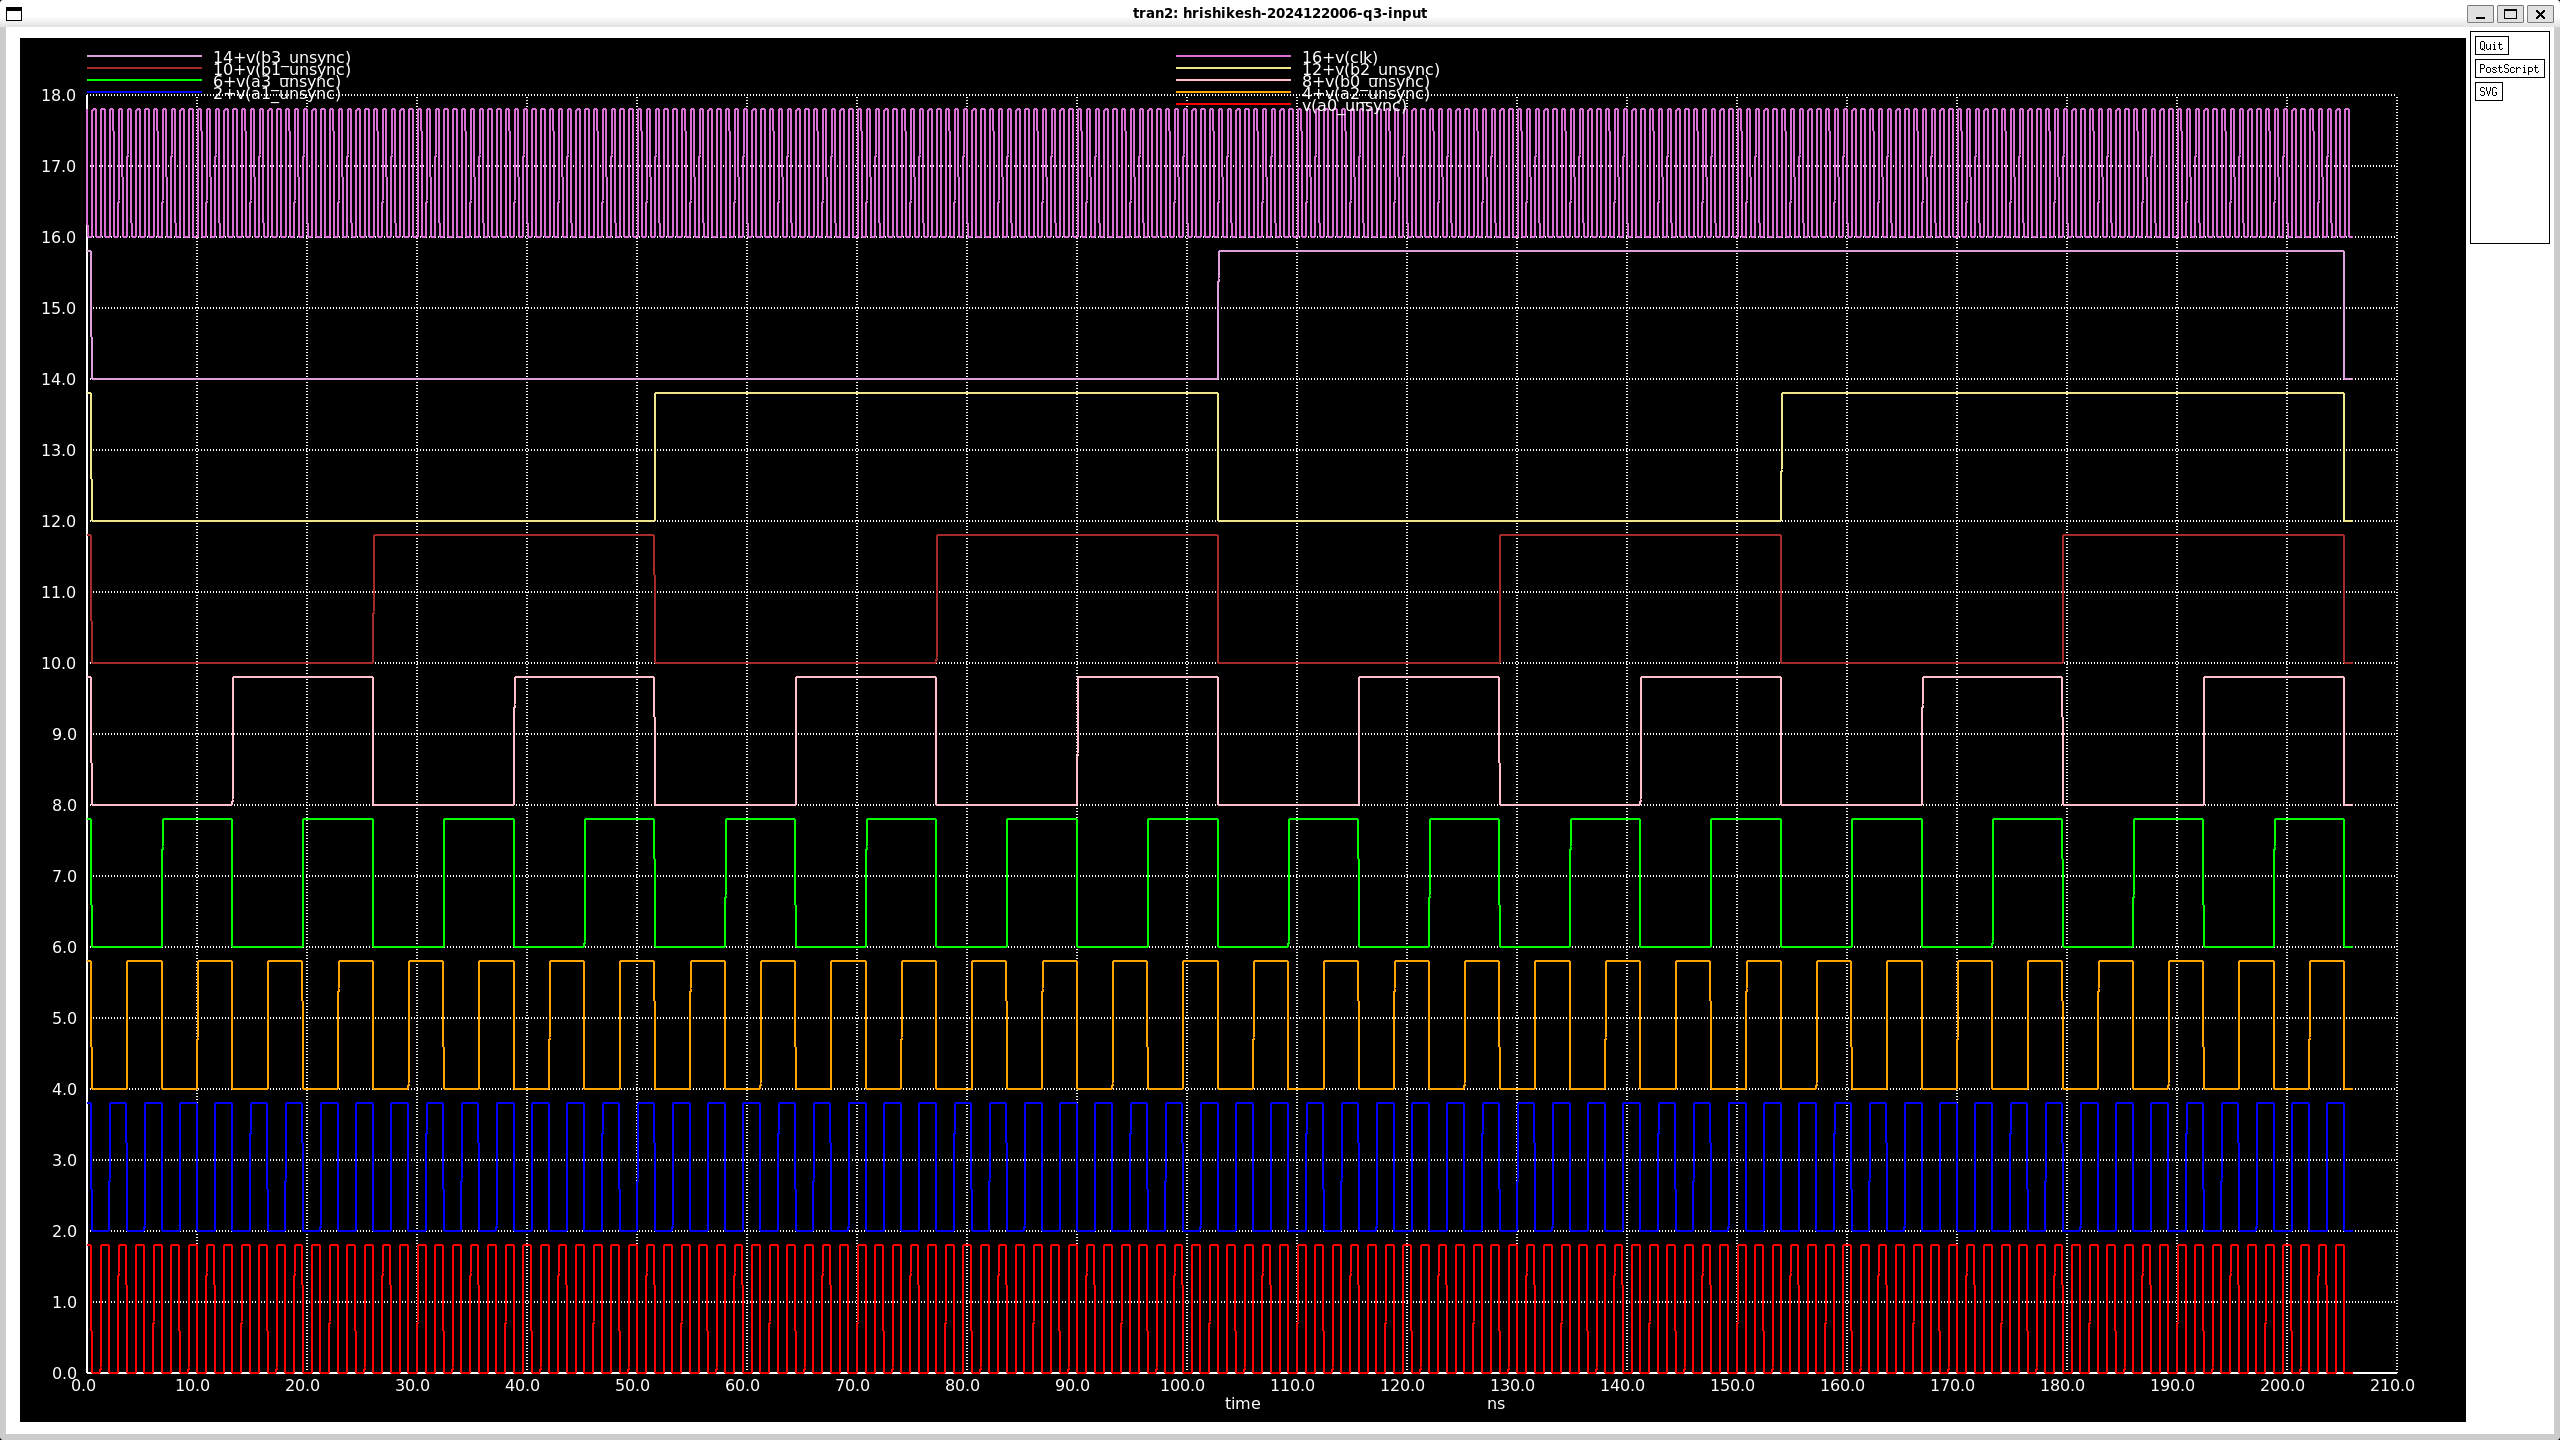
\includegraphics[width=1\linewidth]{modulewise_input.png}
    \caption{Test Inputs a and b}
    \label{fig:enter-label}
\end{figure}
\begin{figure}[H]
    \centering
    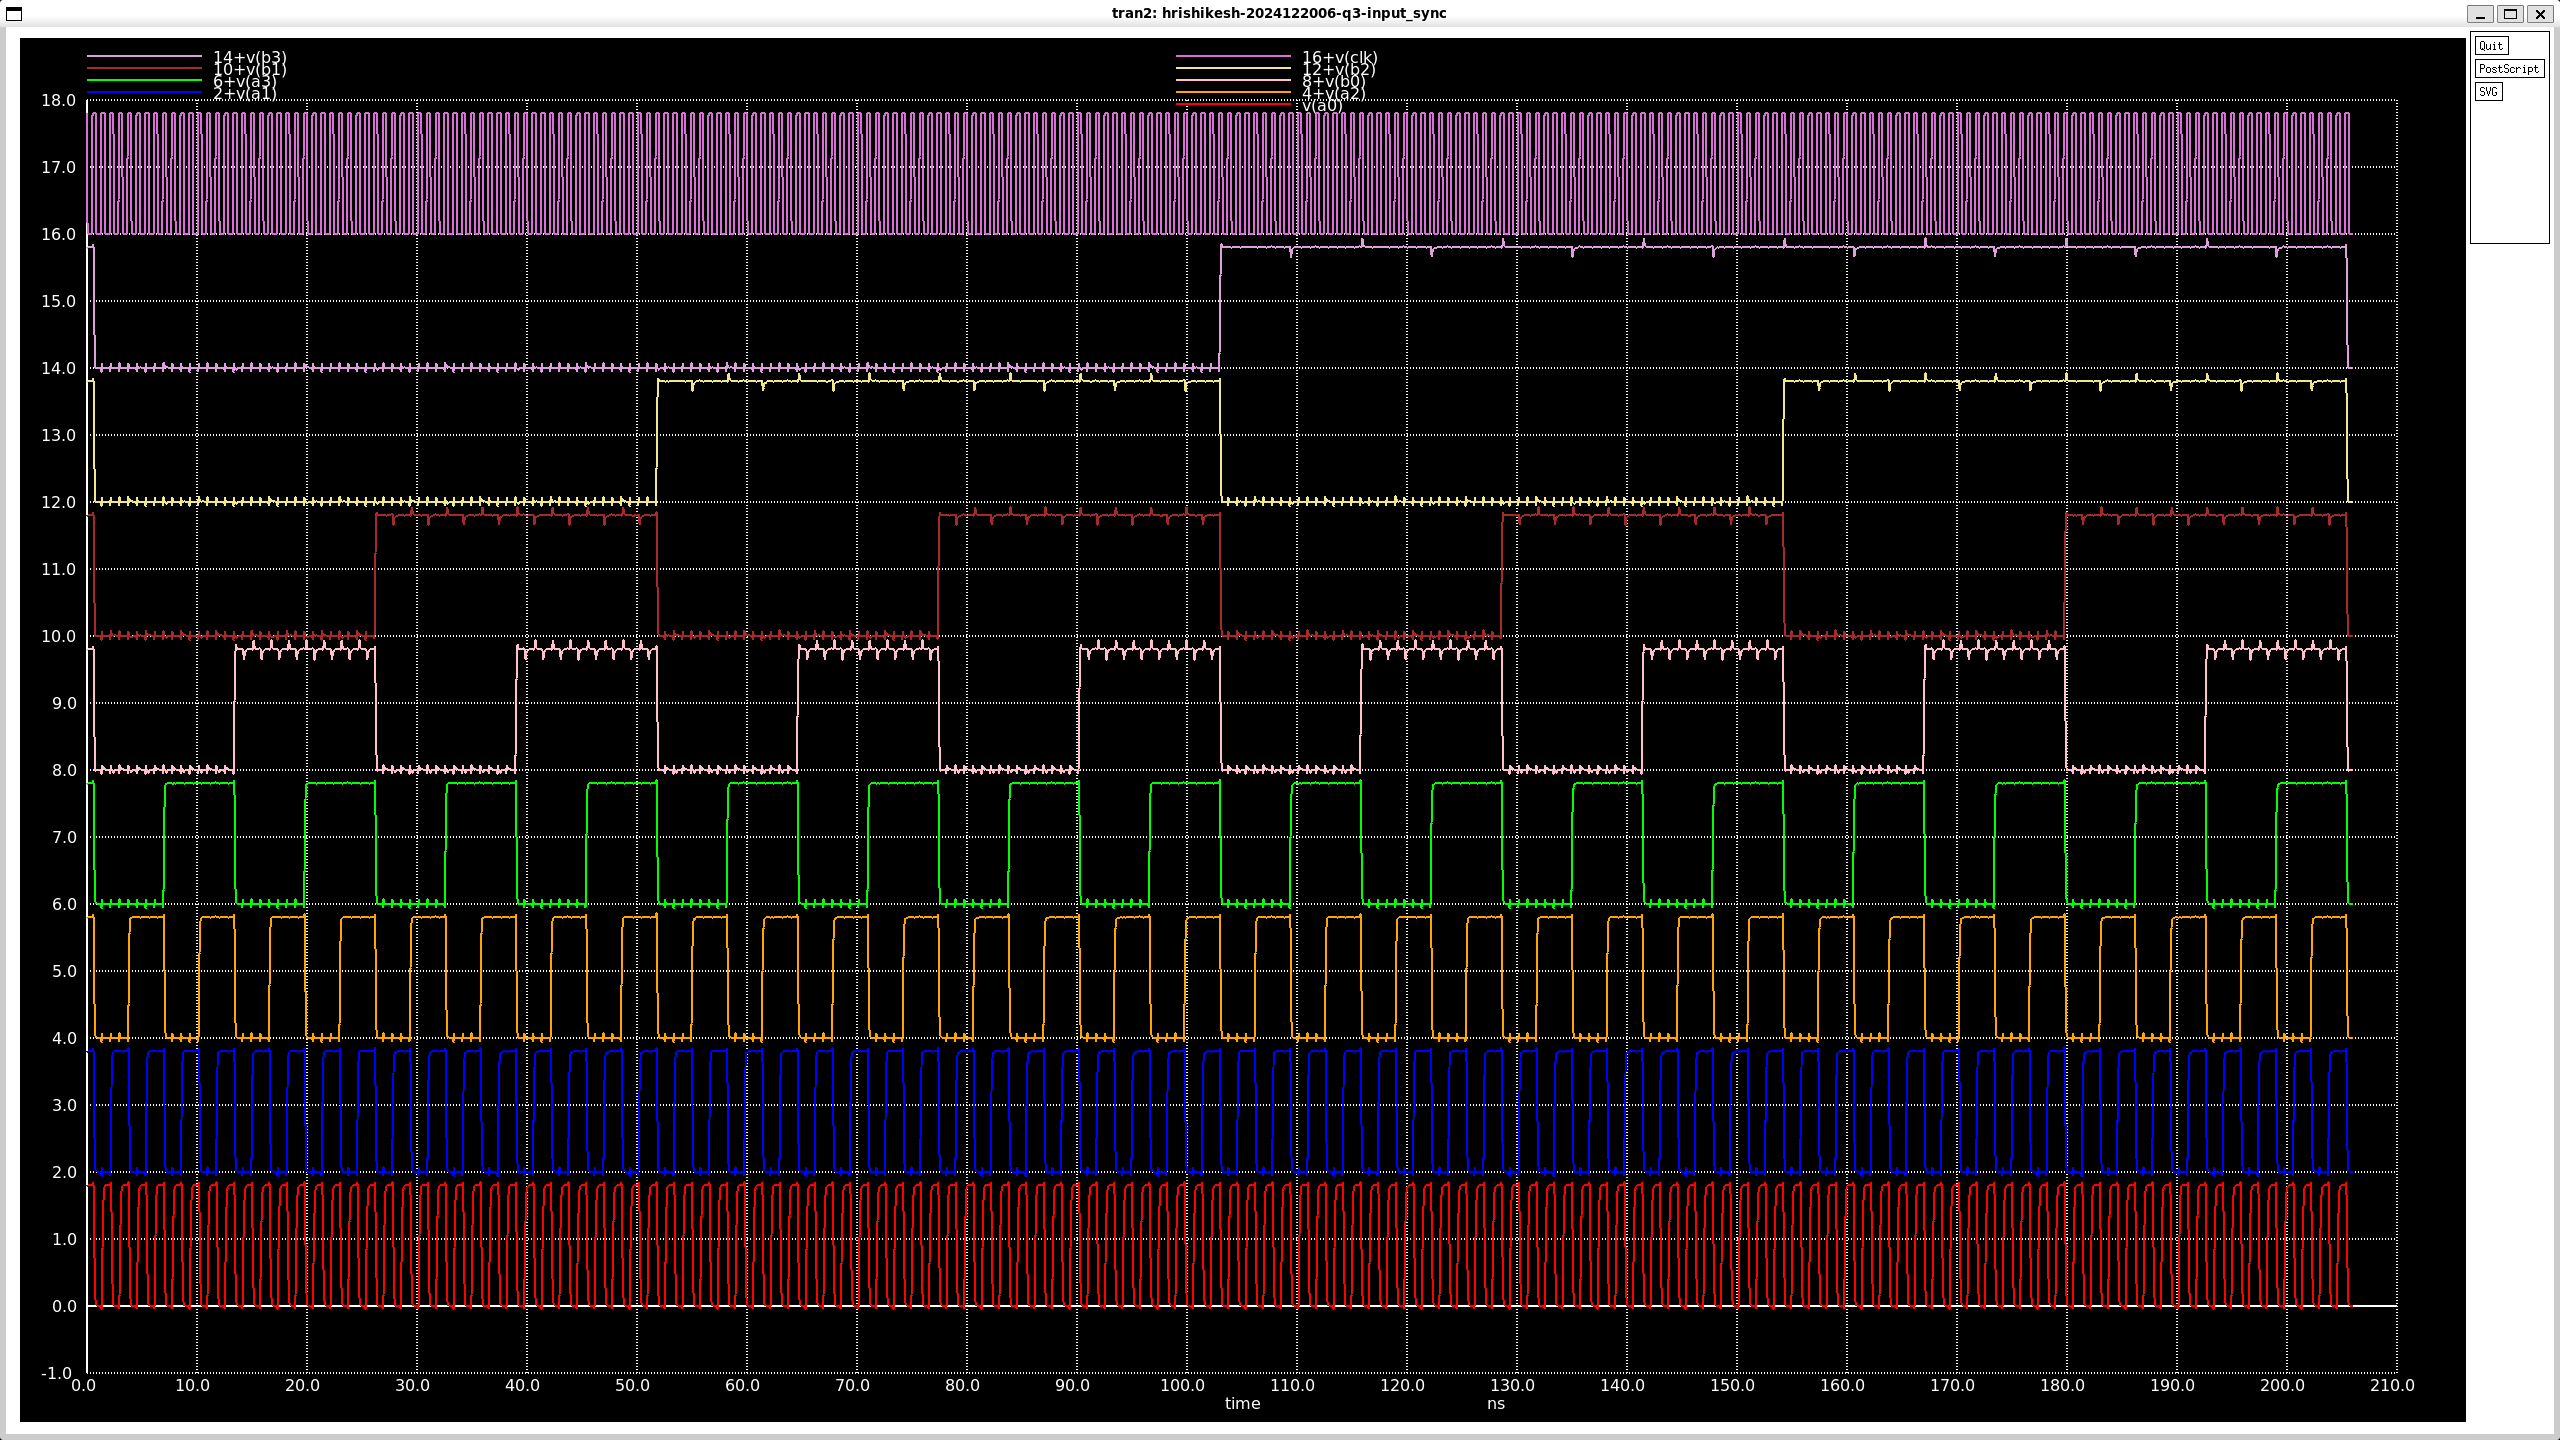
\includegraphics[width=1\linewidth]{modulewise_inputdffout.png}
    \caption{CLA Input}
    \label{fig:enter-label}
\end{figure}
\begin{figure}[H]
    \centering
    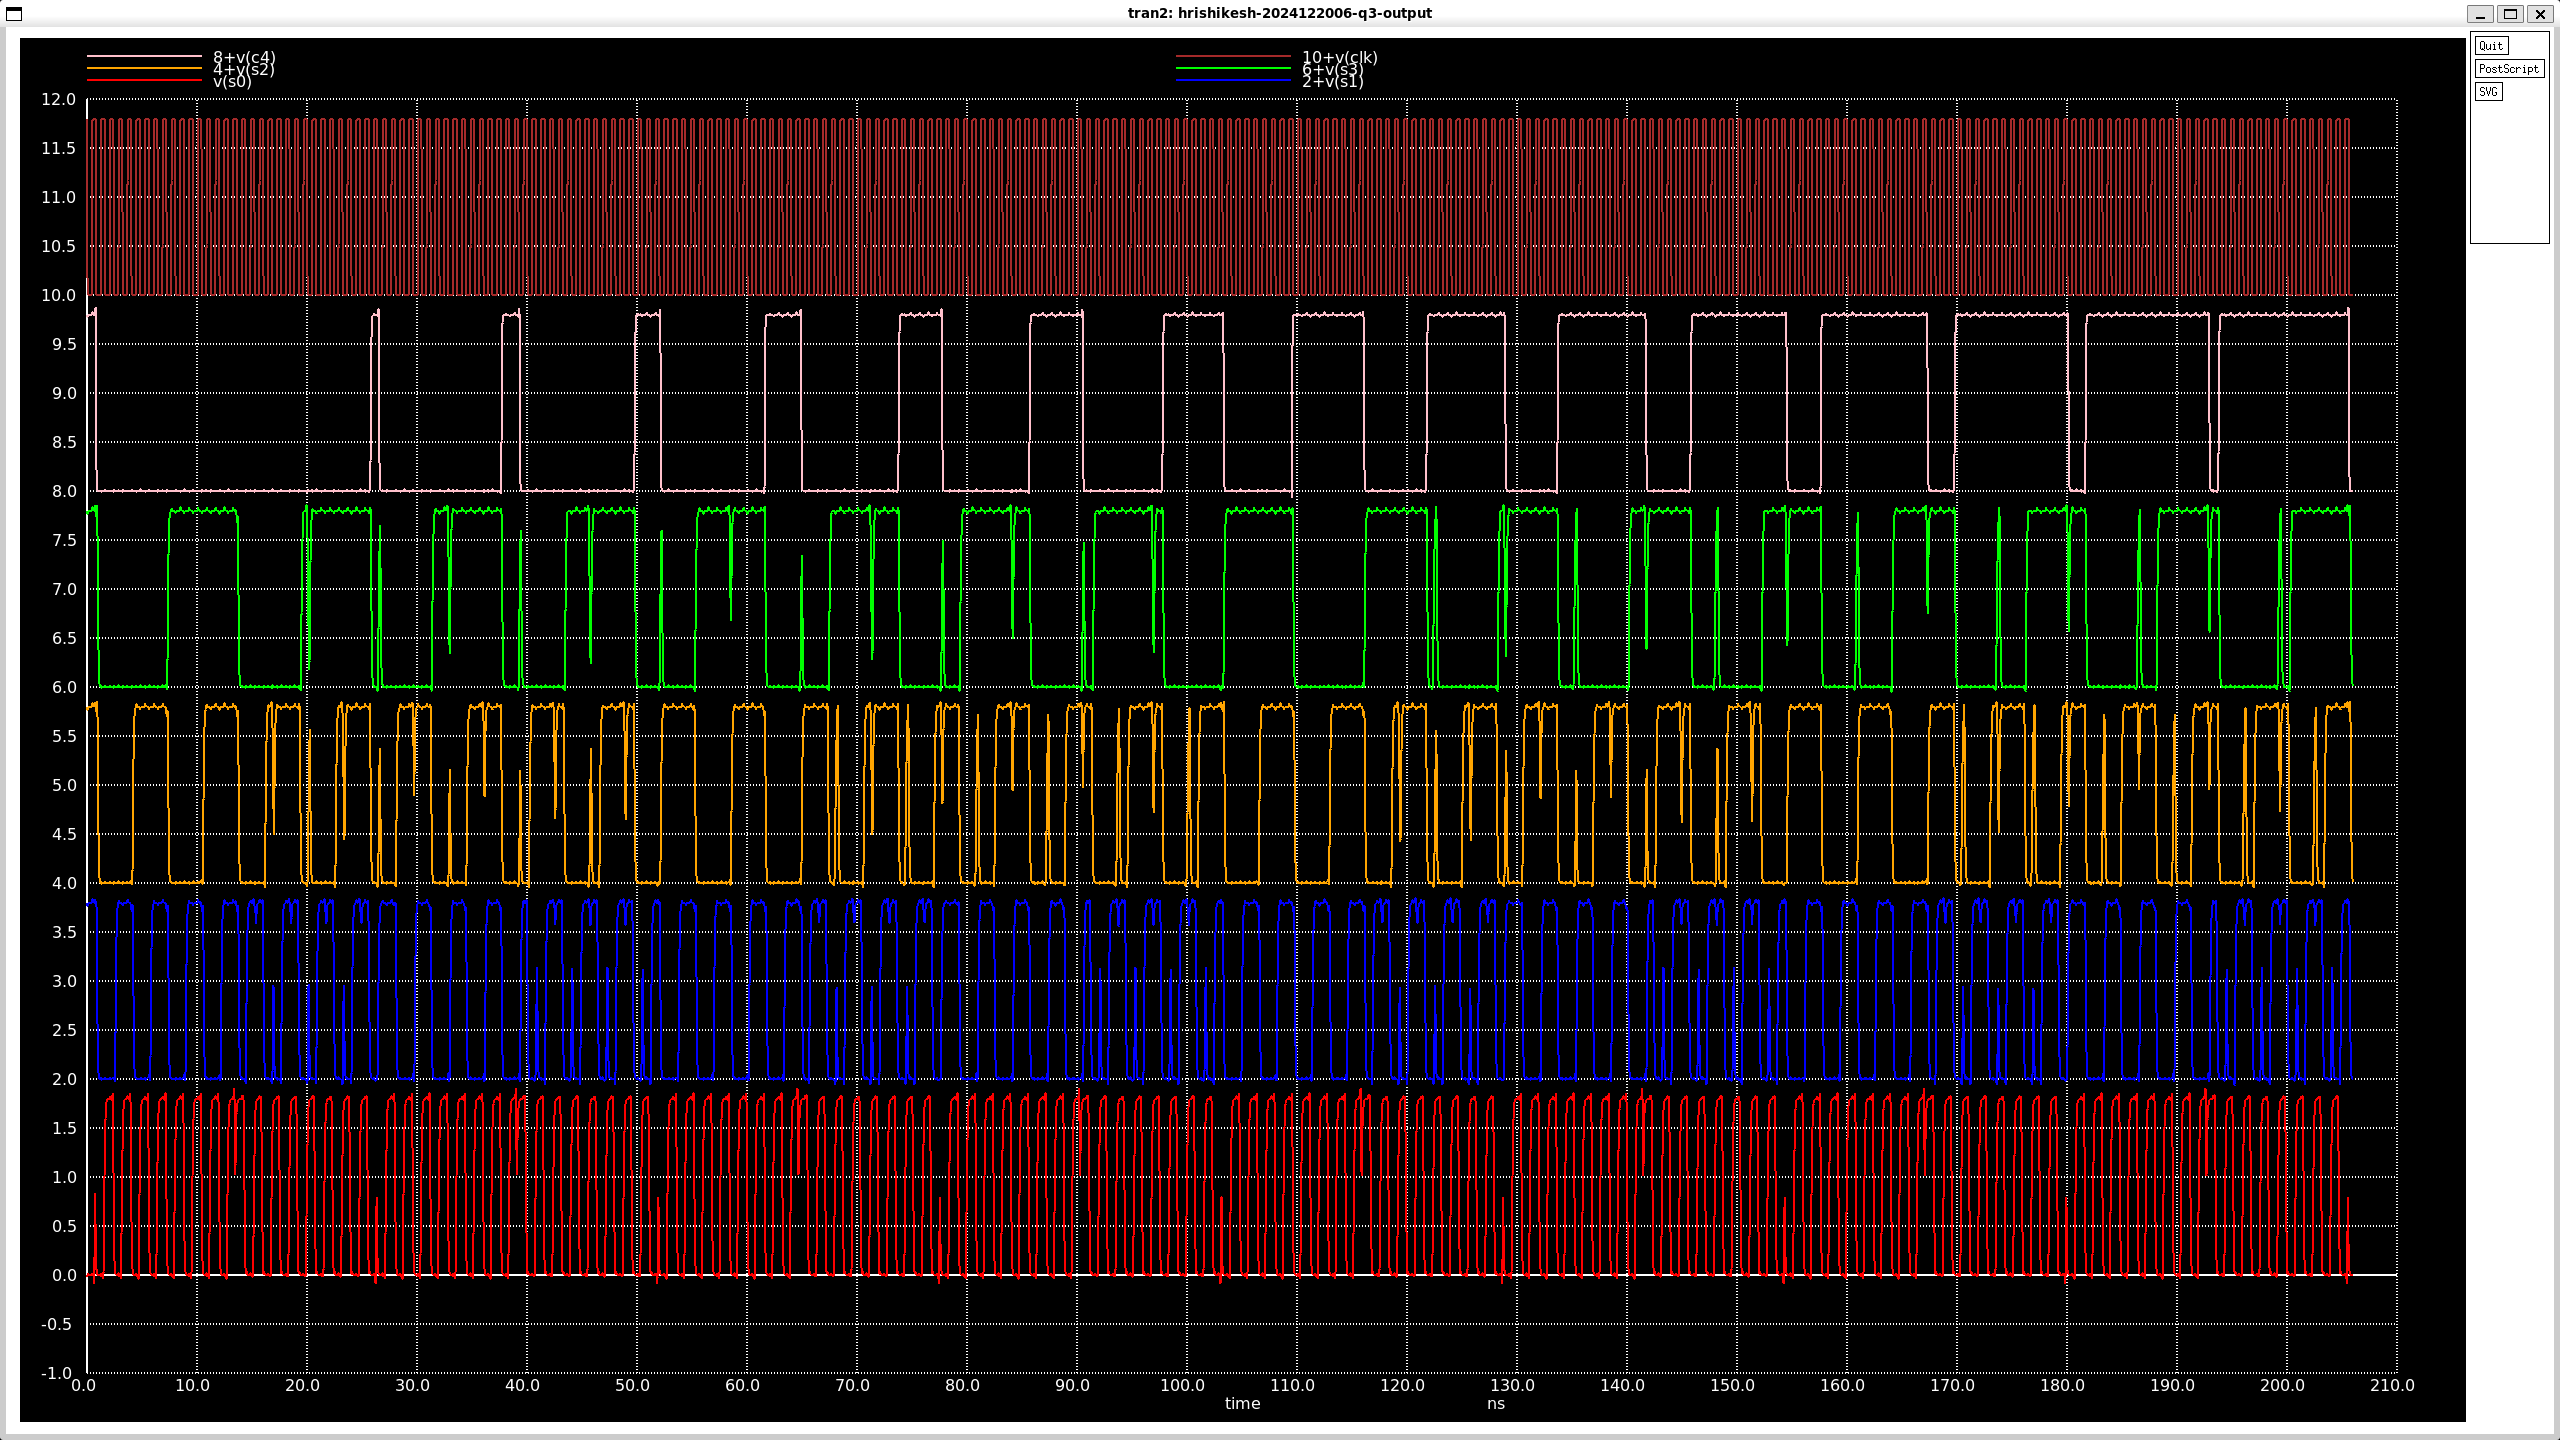
\includegraphics[width=1\linewidth]{modulewise_output.png}
    \caption{CLA Output}
    \label{fig:enter-label}
\end{figure}
\begin{figure}[H]
    \centering
    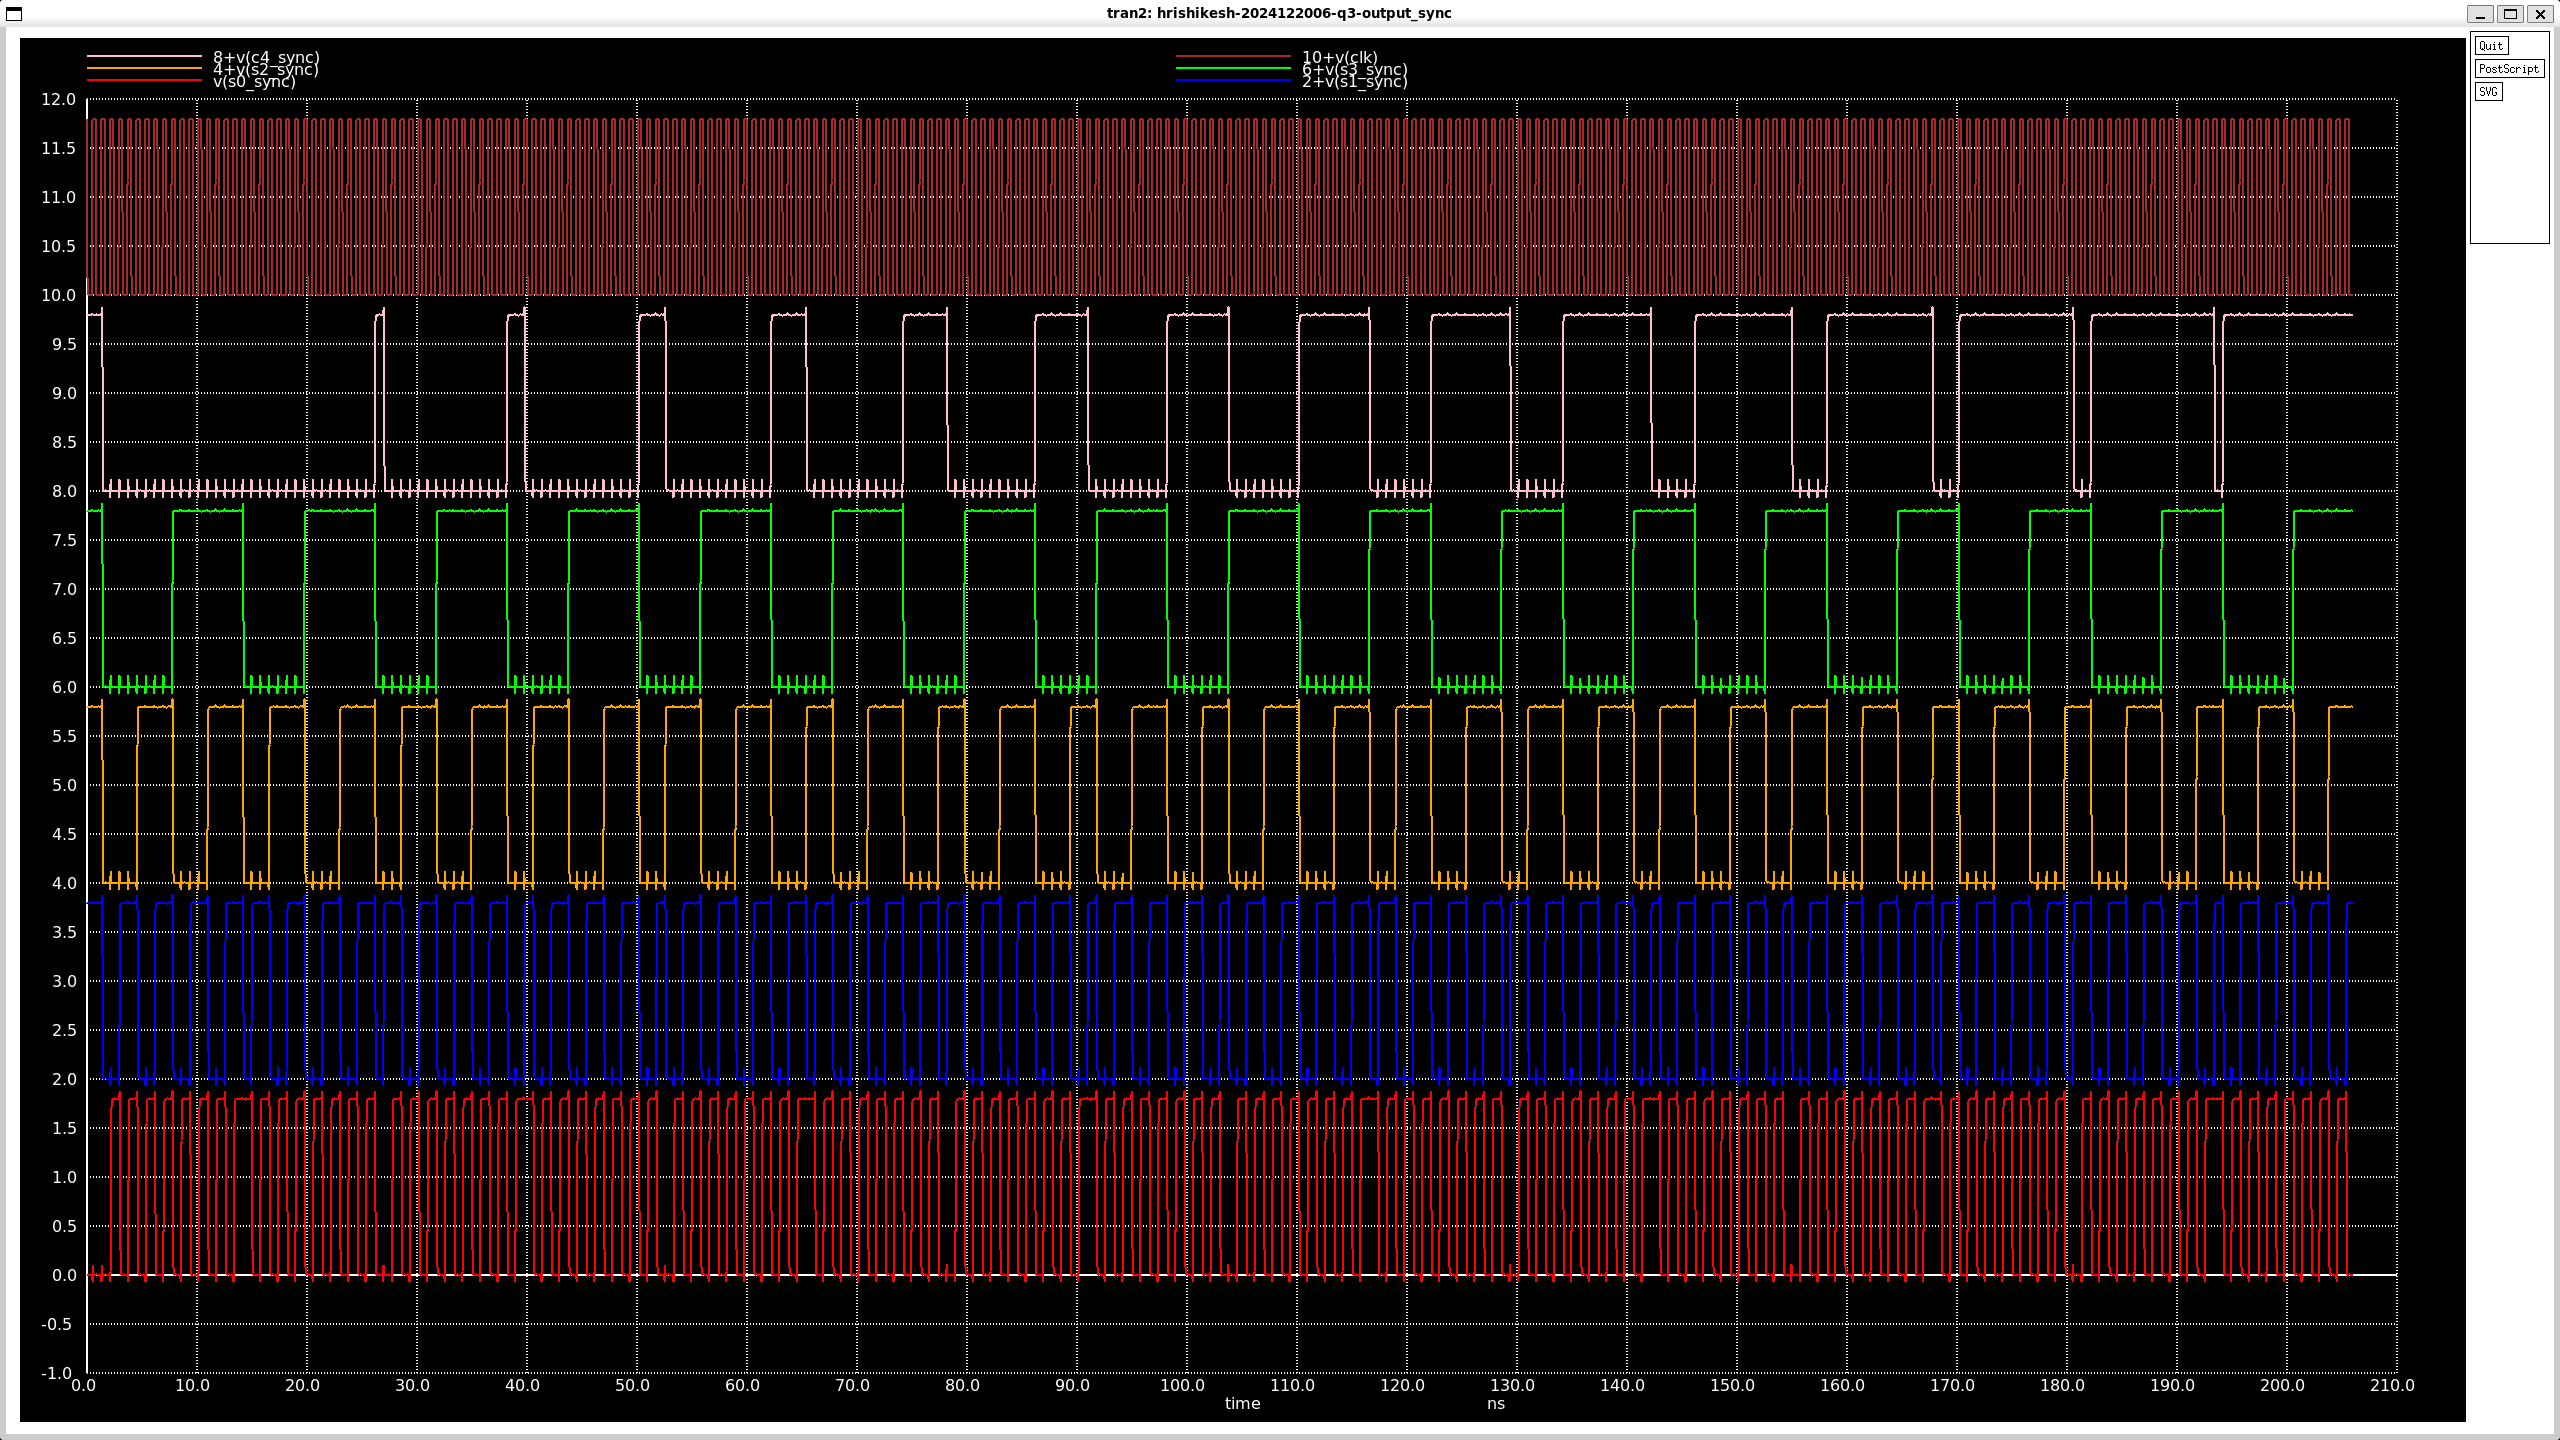
\includegraphics[width=1\linewidth]{modulewise_finalout.png}
    \caption{Final Outputs from DFF}
    \label{fig:enter-label}
\end{figure}
In these diagrams, a0\_unsync,b0\_unsync,.... represent test input provided to input flip flops. a0,b0,.... represent output of input flip flops or the inputs to the CLA. c4,s3,s2,s1,s0 represent outputs of CLA or the inputs to the output flip flops. Finally, c4\_sync,s3\_sync,s2\_sync,s1\_sync,s0\_sync represent the final processed outputs from the output flip flops which are in sync with time. \newline
\textbf{Worst Case Delay: } Worst case delay if obtained on the critical path. Inputs to all other paths are kept constant. Inputs are chosen such that by only toggling the critical path input, the critical path output changes. The rise and fall time propagation delays are noted.\newline
In this case, a0 to s3 is the critical path.
\begin{figure}[H]
    \centering
    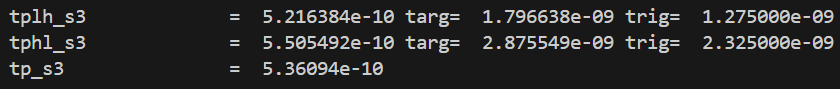
\includegraphics[width=1\linewidth]{modulewise_tp.png}
    \caption{Critical Delays}
    \label{fig:enter-label}
\end{figure}
The case with maximum $t_p$ (lh or hl) was chosen to calculate Maximum Clock Frequency.
\[
    t_{CLK} \geq t_p + t_{setup} + t_{pcq} = 551 + 24 + 147 = 722 ps
\]
But certain flaws were noticed at exact time period of 722 ps, therefore for reliable operation a time period of 800 ps was chosen. This equates to 1.25 GHZ of max clock frequency.

\section{Final Layout}
Floor plan of the layout for the complete circuit is shown below. 
\begin{figure}[H]
    \centering
    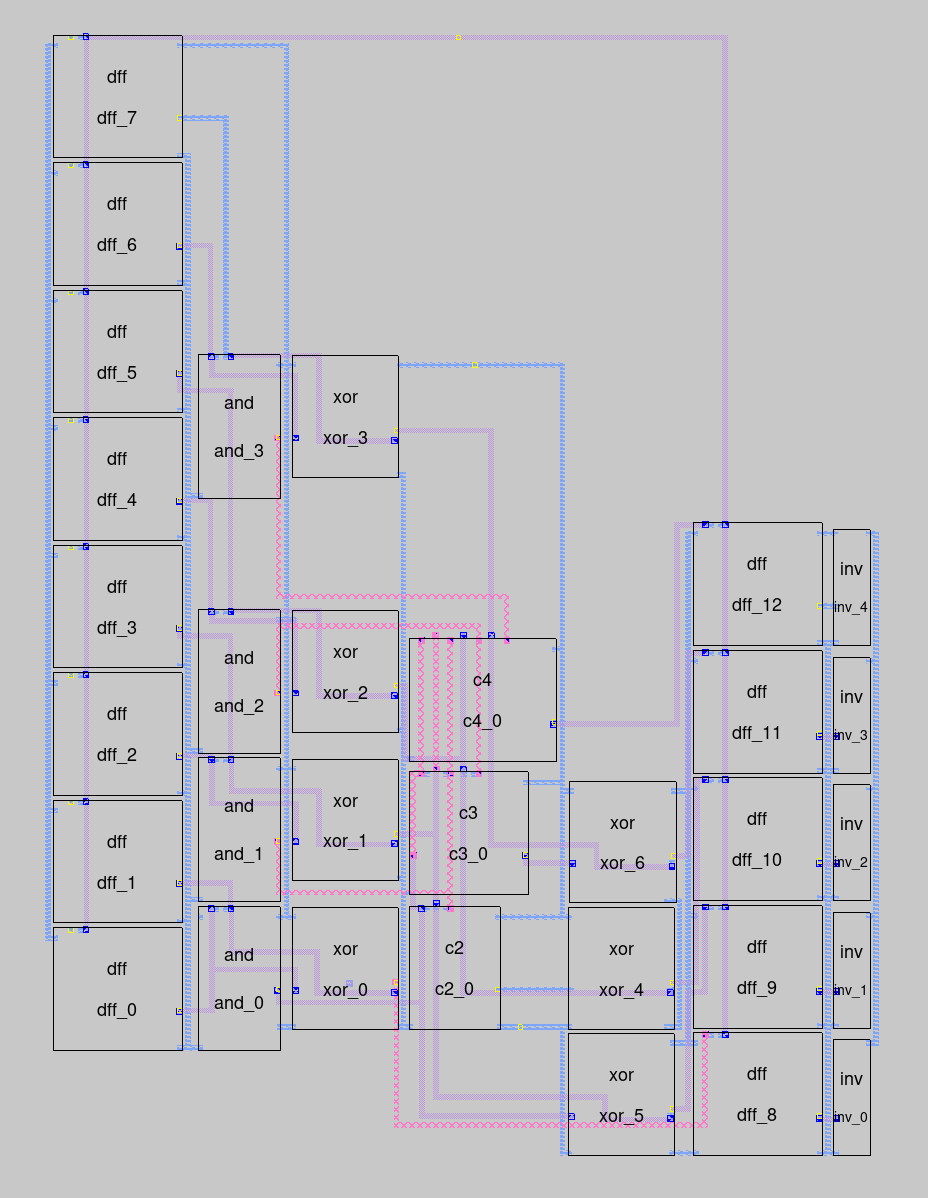
\includegraphics[width=0.9\linewidth]{floor_plan.png}
    \caption{Floor Plan}
    \label{fig:enter-label}
\end{figure}
\begin{figure}[H]
    \centering
    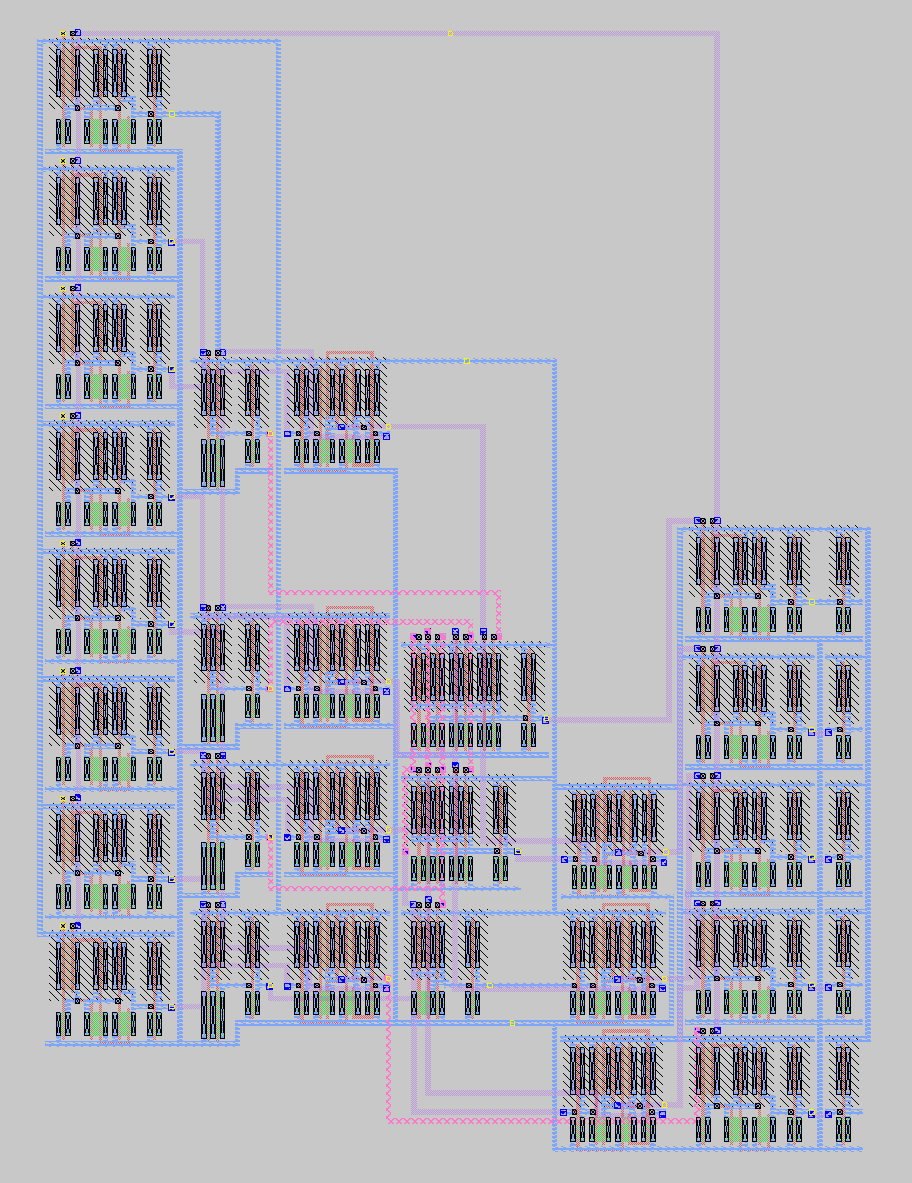
\includegraphics[width=0.9\linewidth]{FinalLayout.png}
    \caption{Final Layout}
    \label{fig:enter-label}
\end{figure}
\begin{table}[H]
\begin{tabular}{|c|c|c|}
\hline
Horizontal Pitch & Vertical Pitch & Area\\ \hline
64.08 microns & 86.31 microns & 5.5307448e-10 $m^2$ \\ \hline
\end{tabular}
\end{table}
Simulations discussed above are repeated for the extracted netlist of final layout.
\begin{figure}[H]
    \centering
    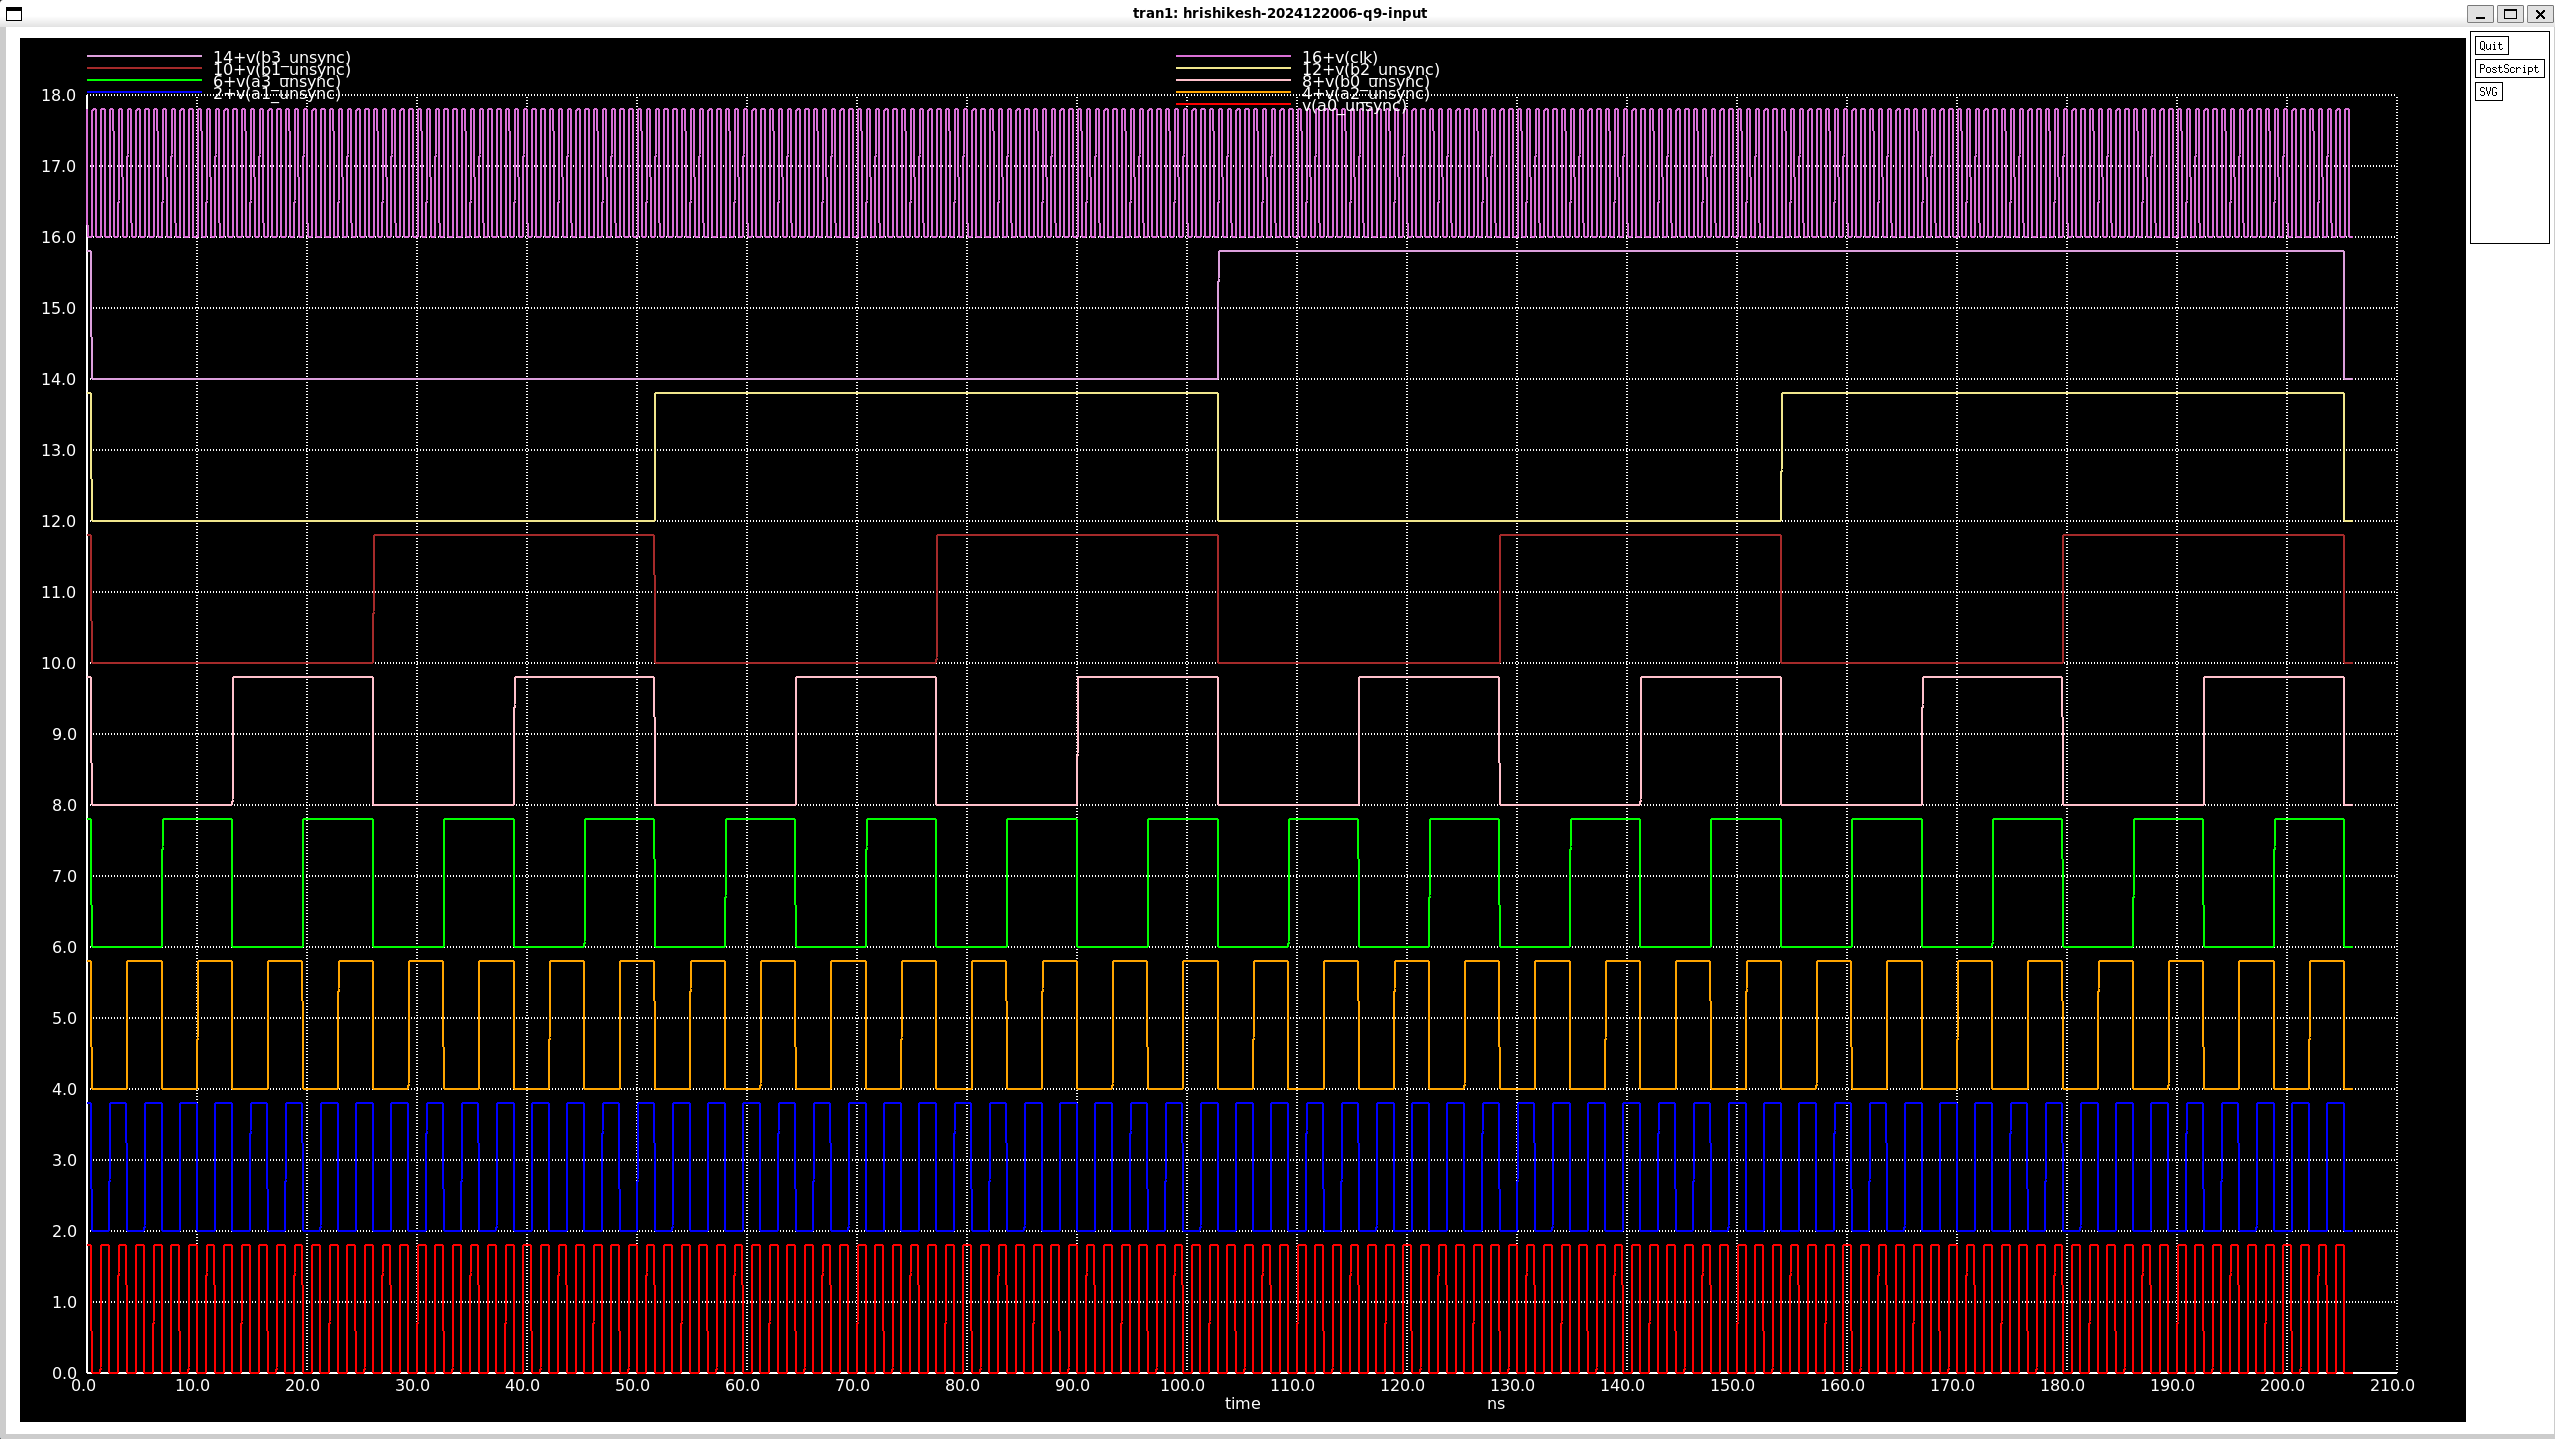
\includegraphics[width=1\linewidth]{q9_testinput.png}
    \caption{Test Inputs a and b}
    \label{fig:enter-label}
\end{figure}
\begin{figure}[H]
    \centering
    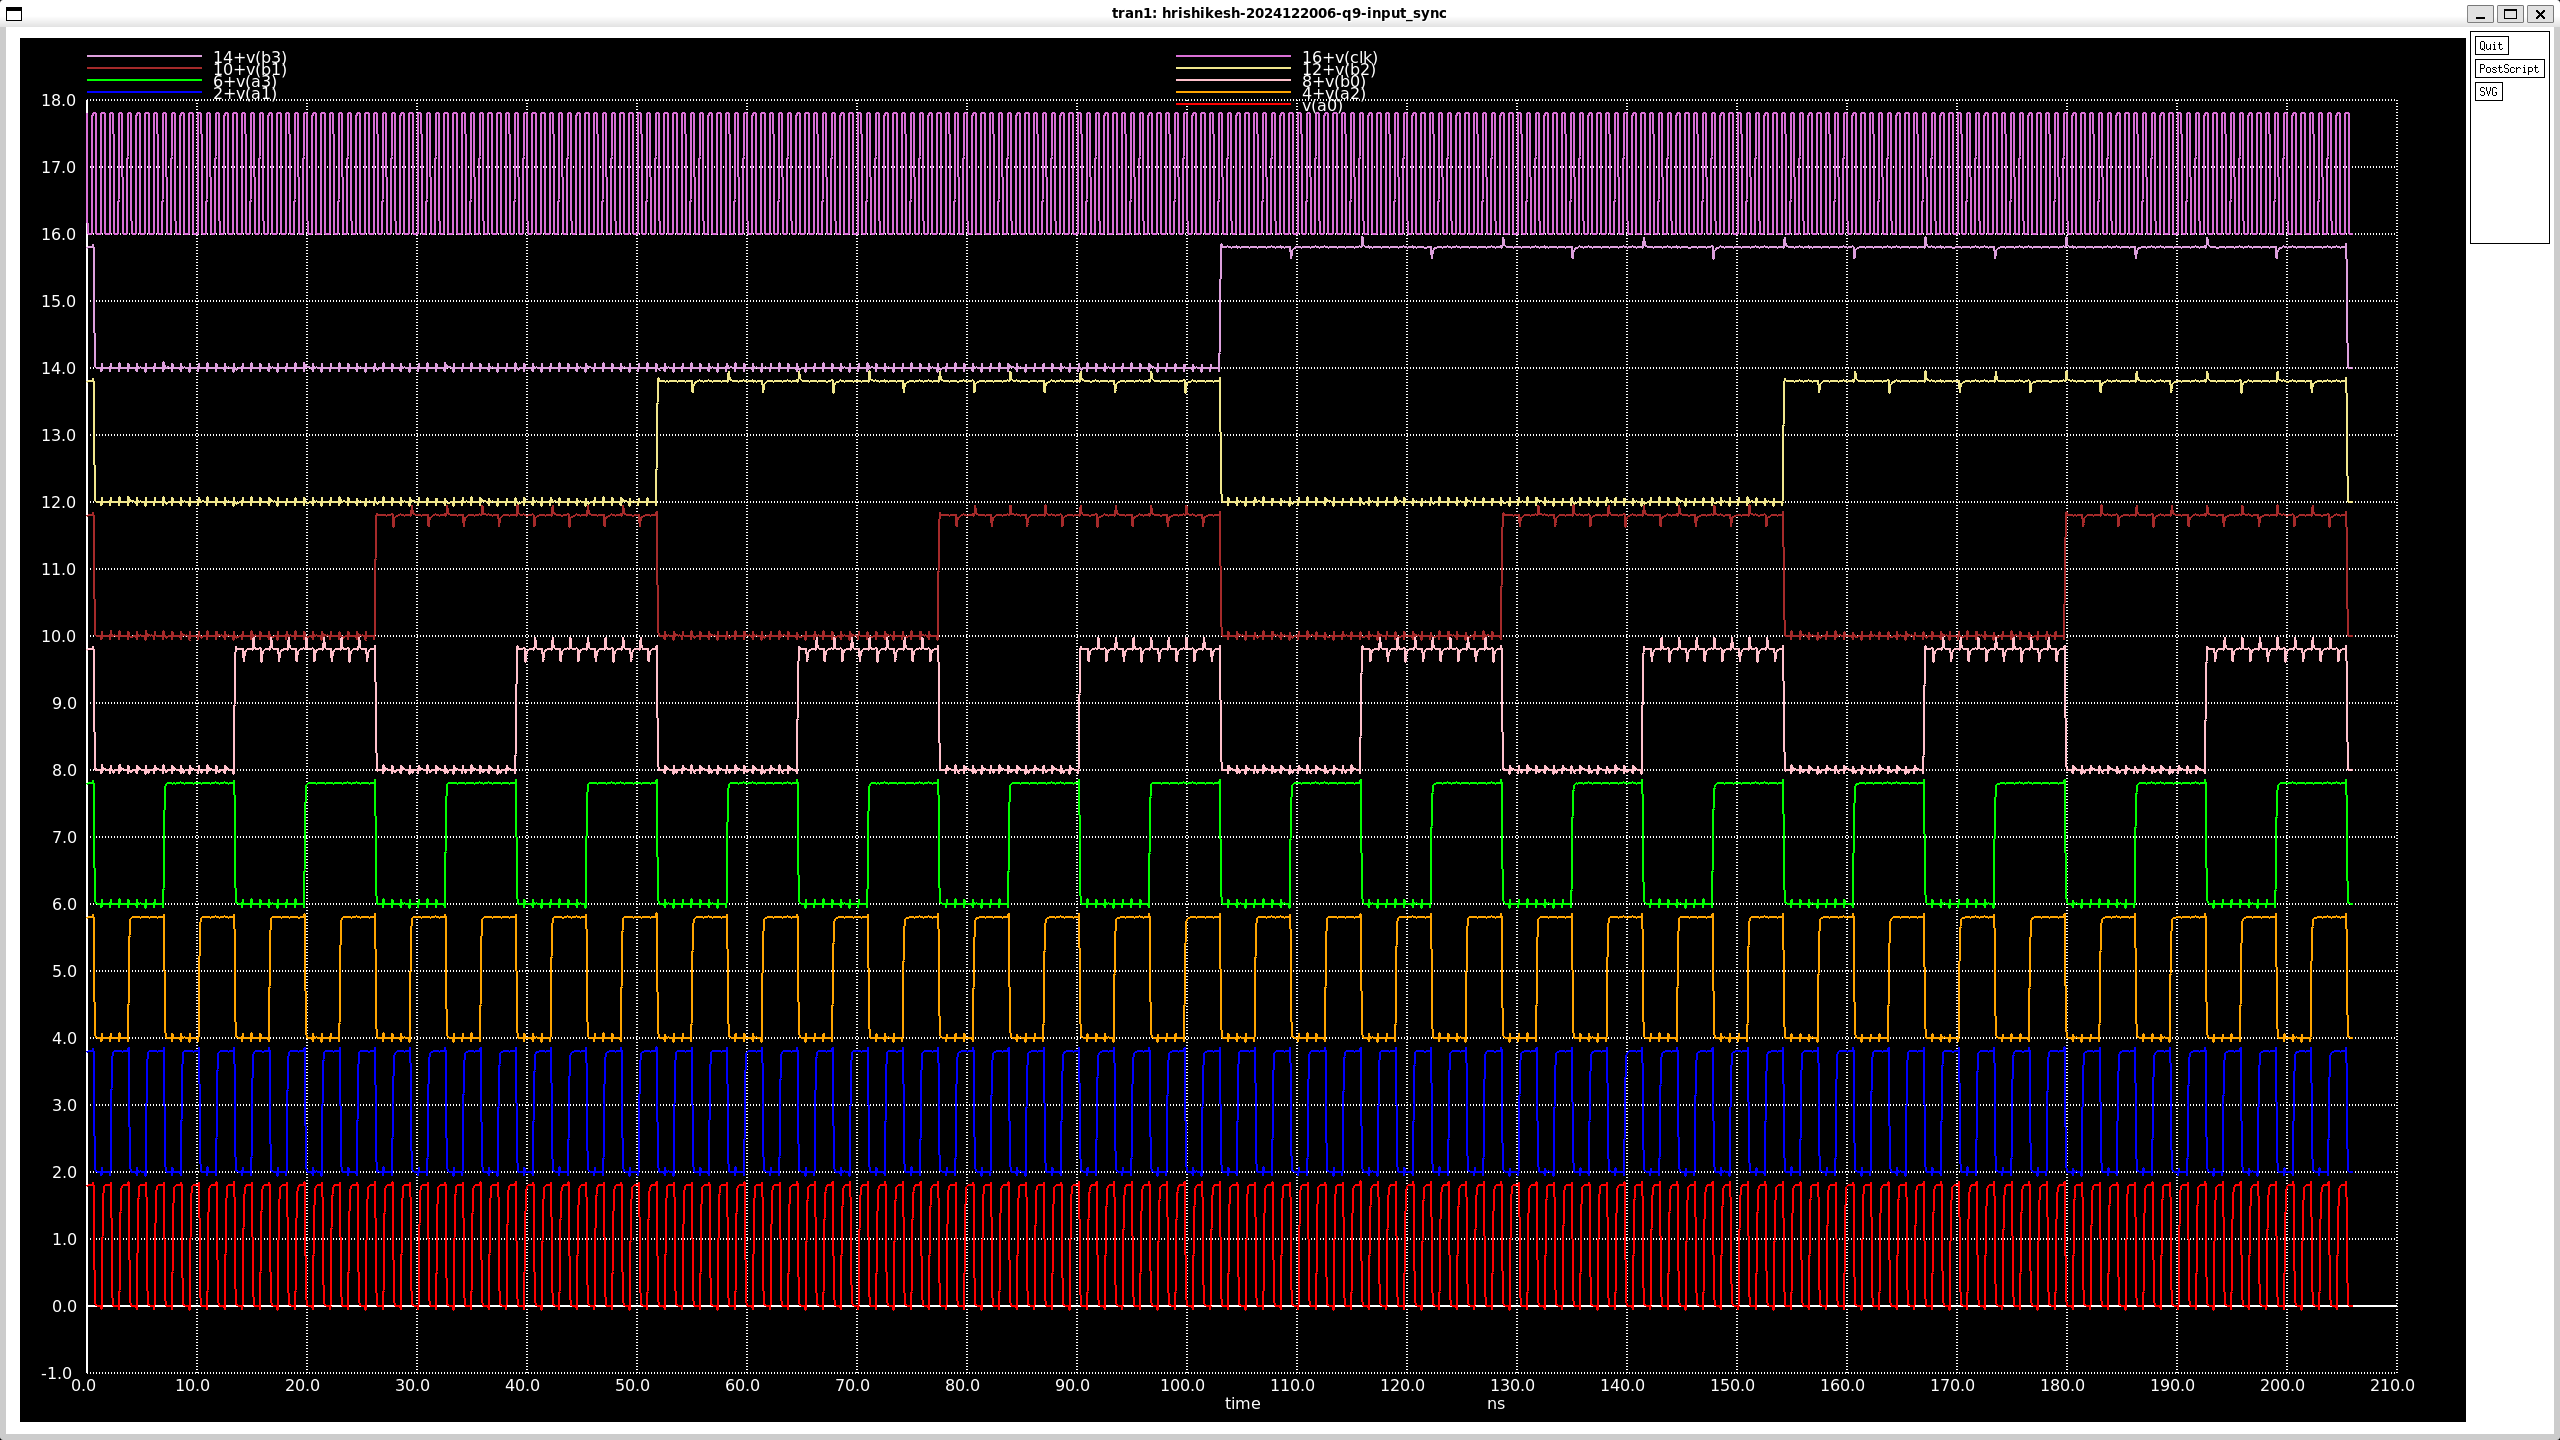
\includegraphics[width=1\linewidth]{q9_inputsync.png}
    \caption{CLA Input}
    \label{fig:enter-label}
\end{figure}
\begin{figure}[H]
    \centering
    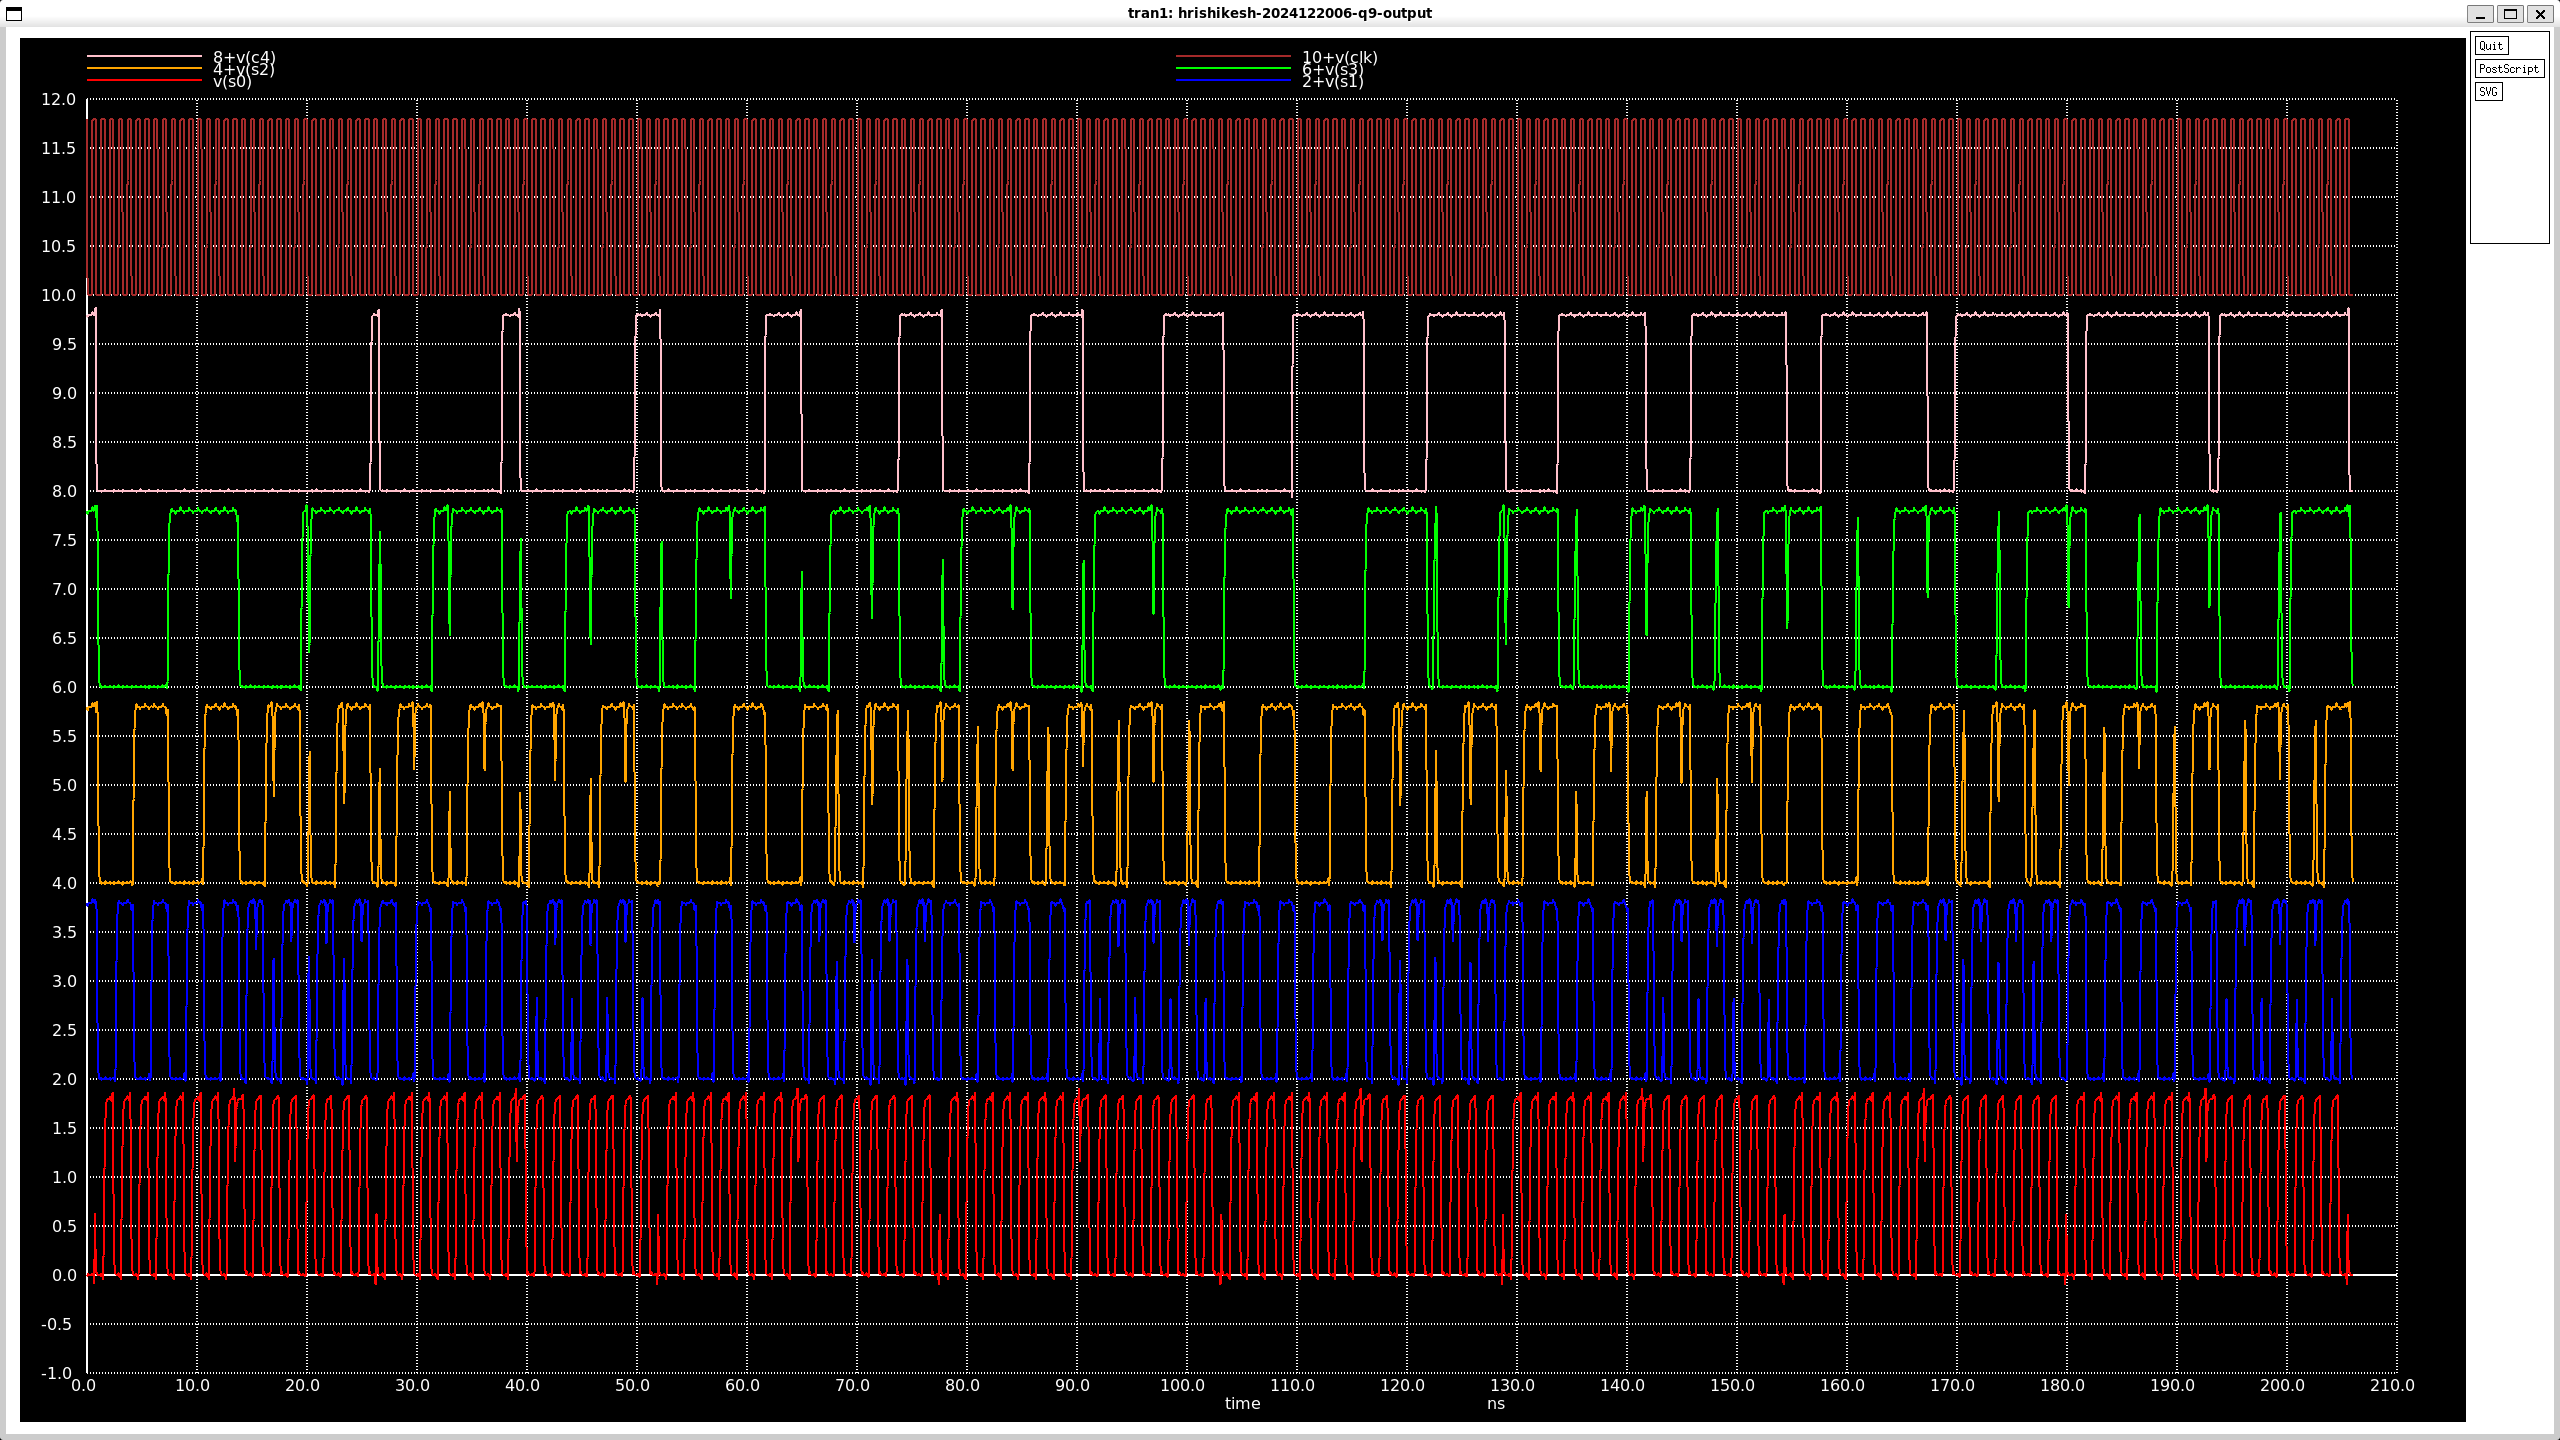
\includegraphics[width=1\linewidth]{q9_claout.png}
    \caption{CLA Output}
    \label{fig:enter-label}
\end{figure}
\begin{figure}[H]
    \centering
    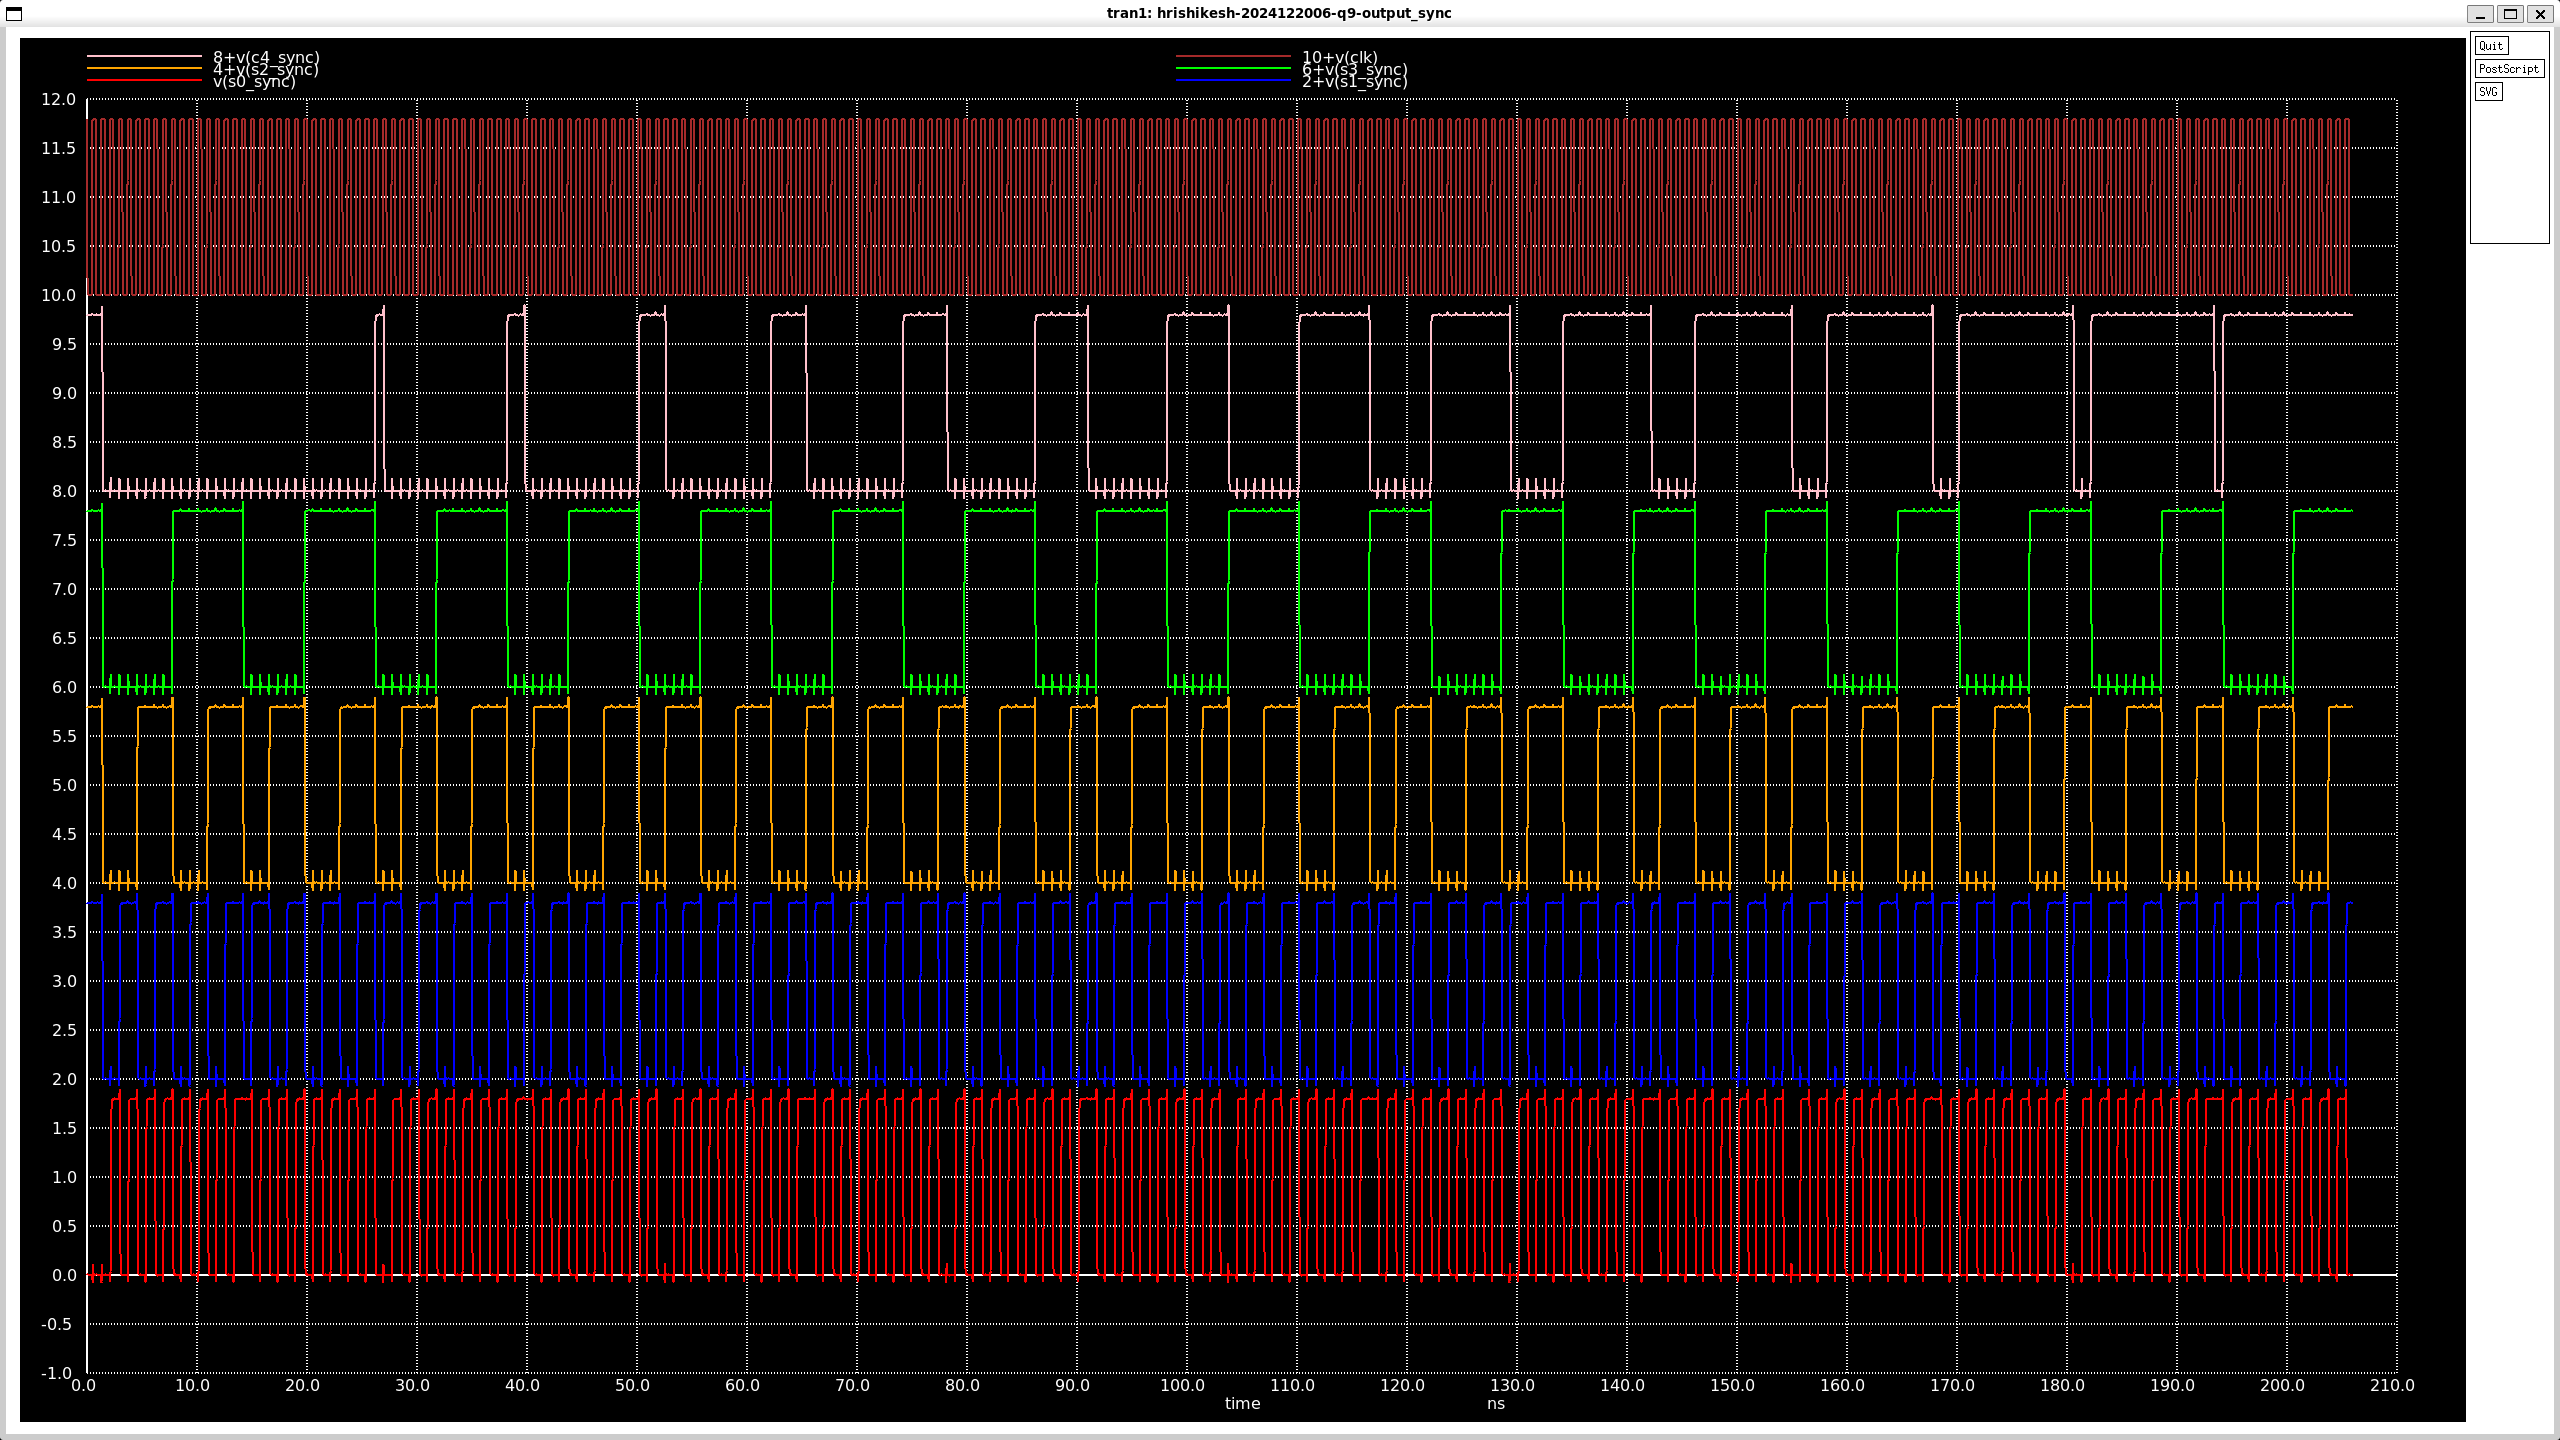
\includegraphics[width=1\linewidth]{q9_finalout.png}
    \caption{Final Outputs from DFF}
    \label{fig:enter-label}
\end{figure}
\begin{figure}[H]
    \centering
    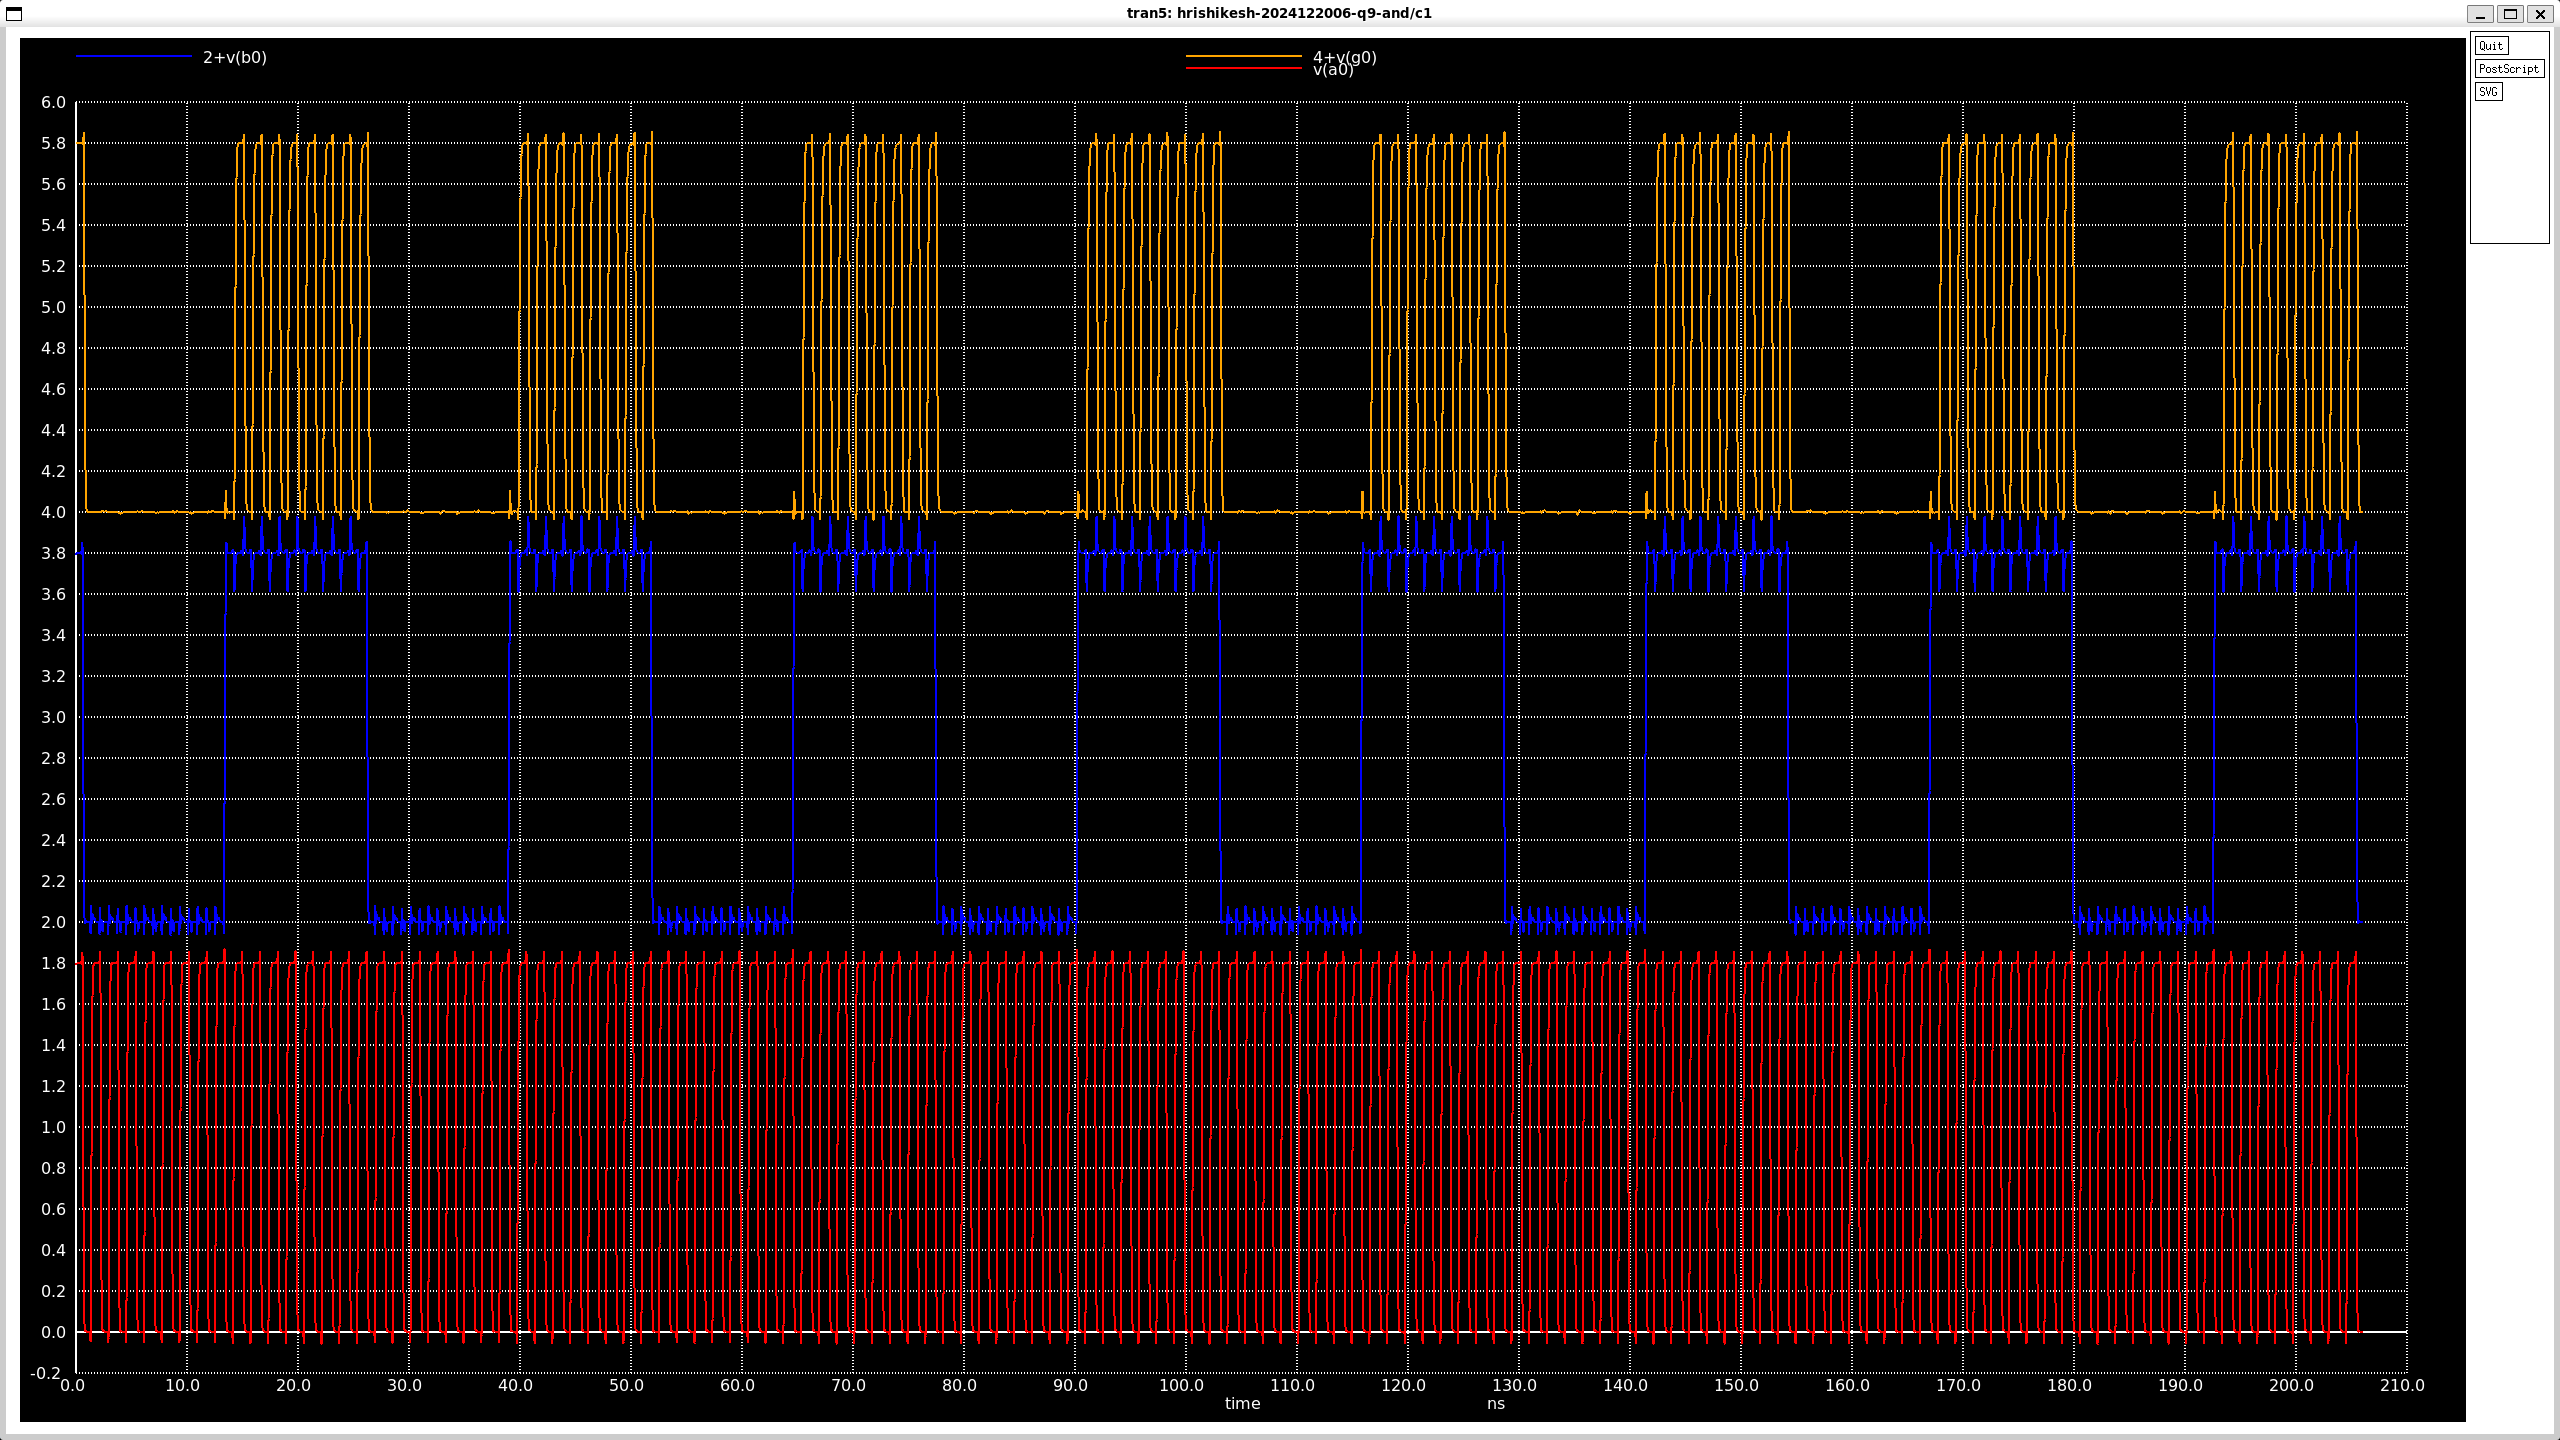
\includegraphics[width=1\linewidth]{final_and.png}
    \caption{AND Gate}
    \label{fig:enter-label}
\end{figure}
\begin{figure}[H]
    \centering
    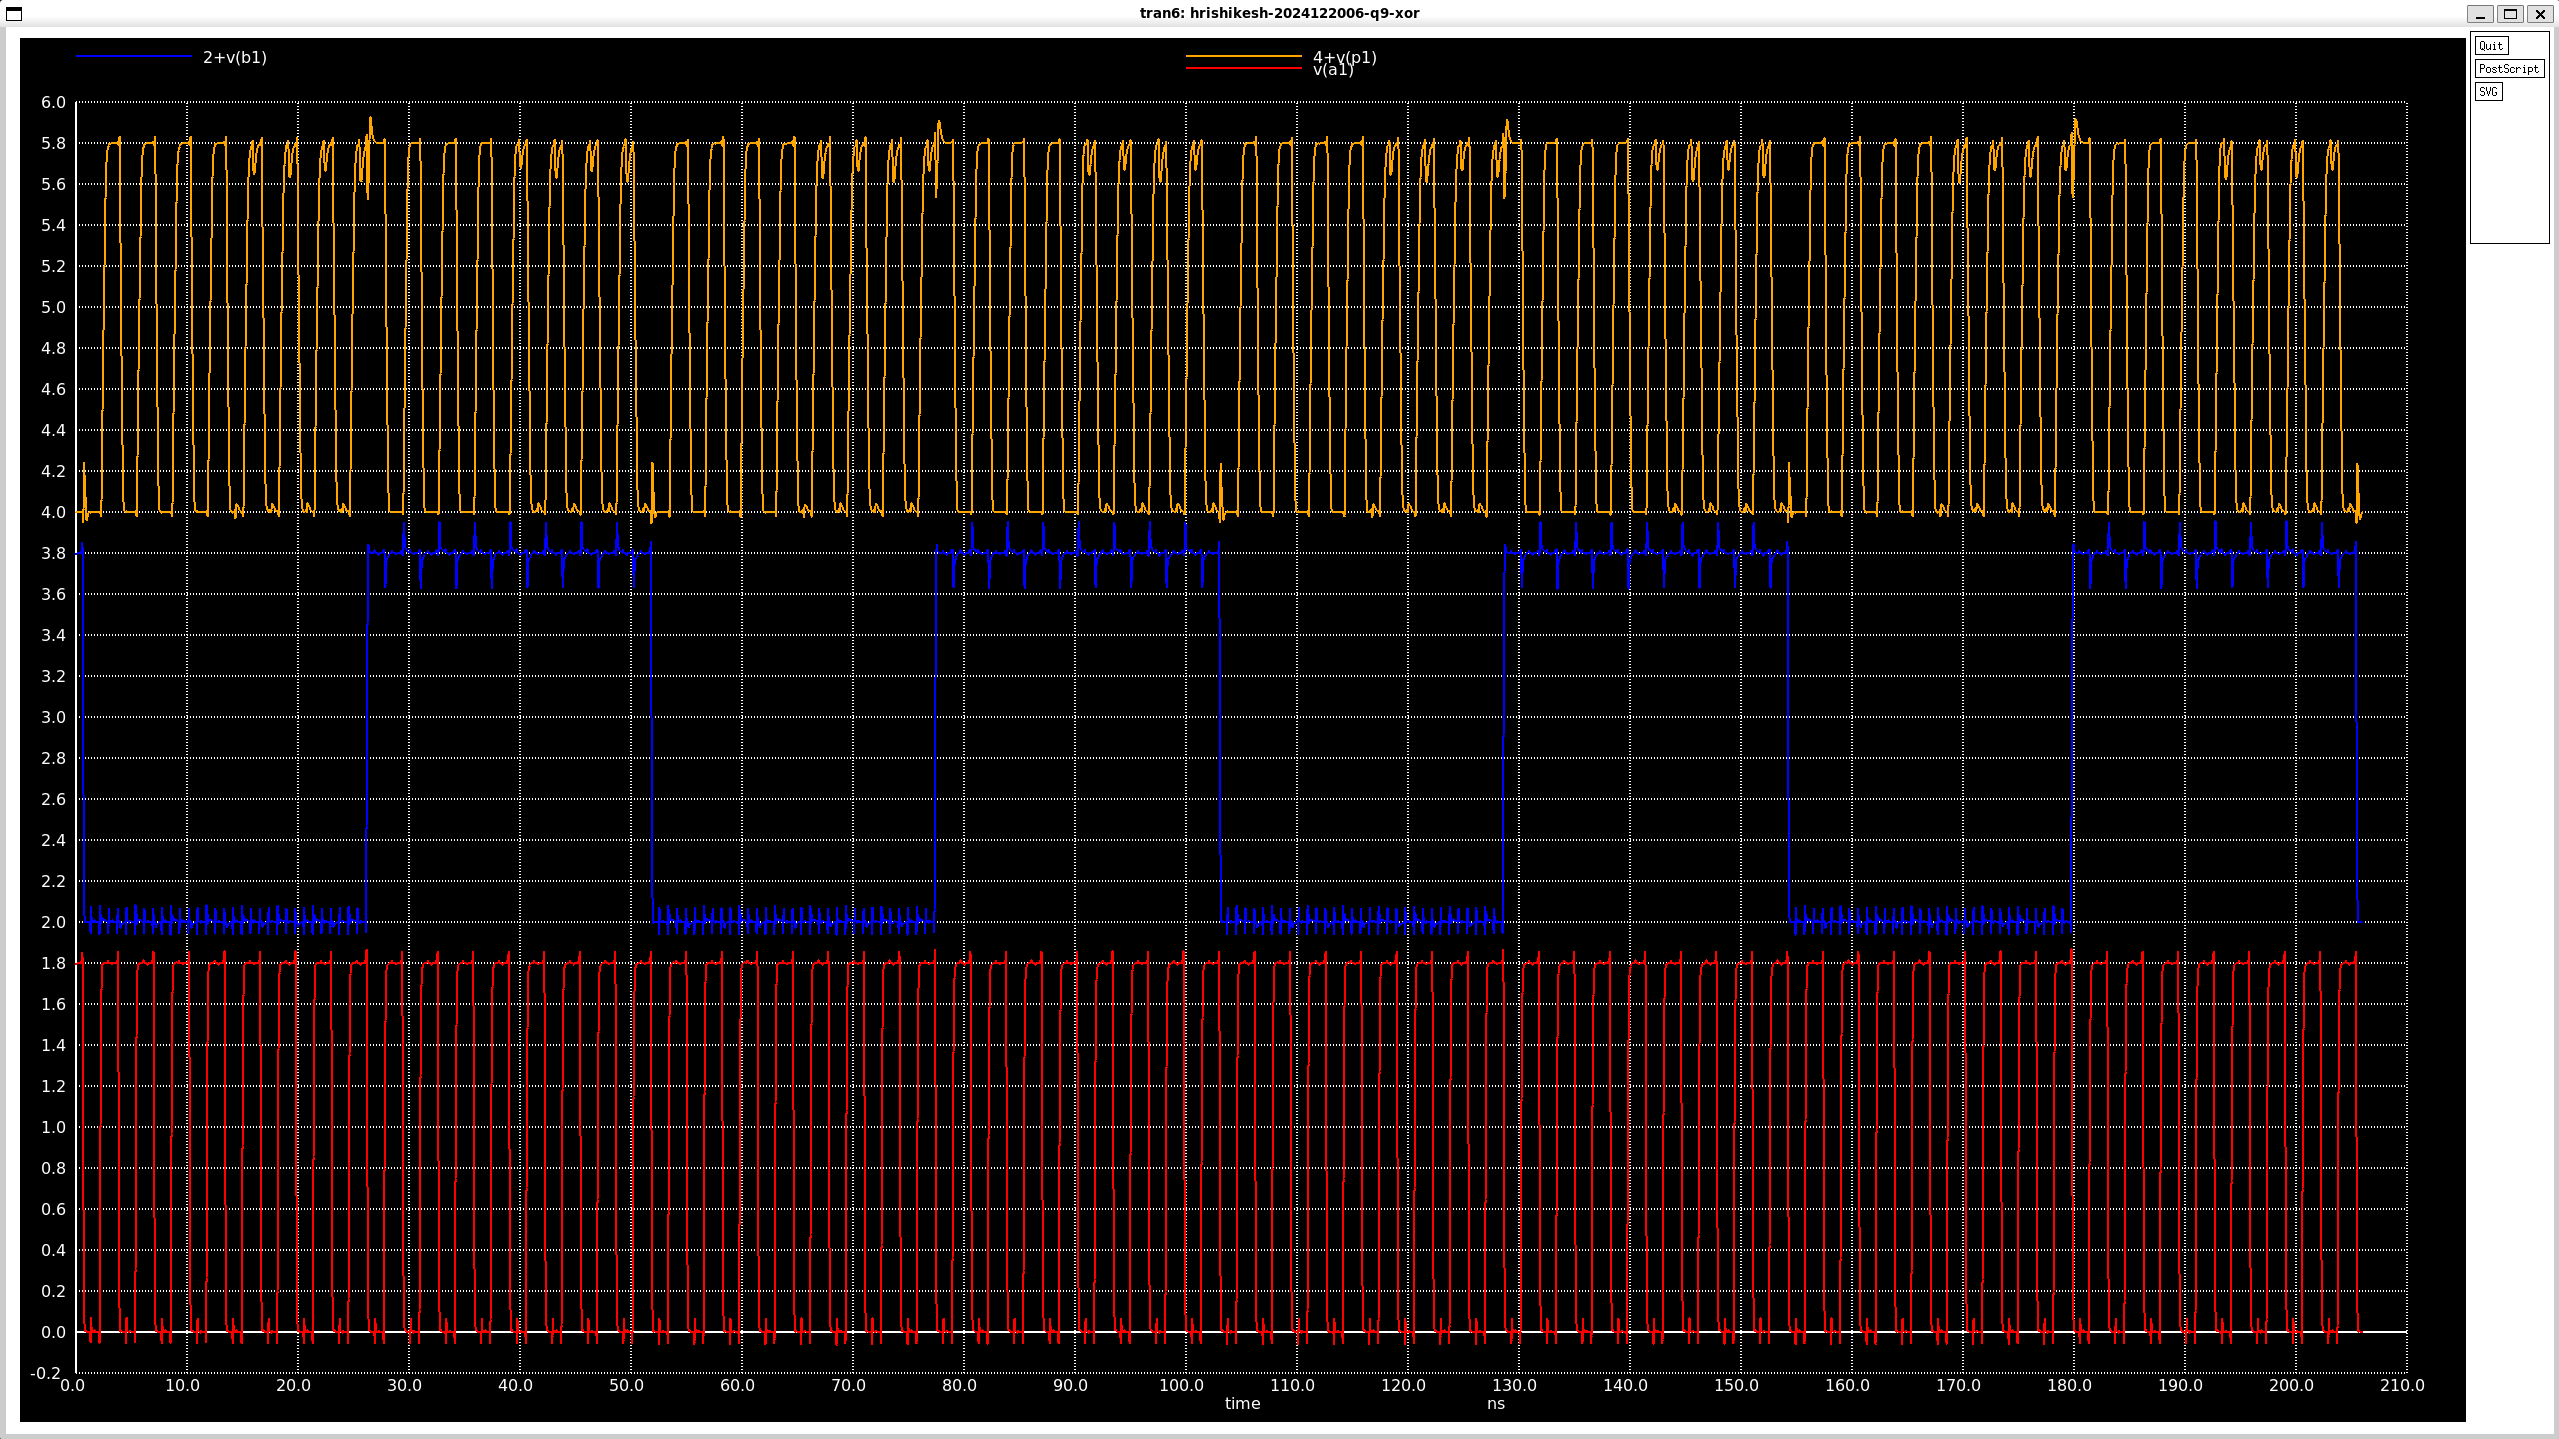
\includegraphics[width=1\linewidth]{final_xor.png}
    \caption{XOR Gate}
    \label{fig:enter-label}
\end{figure}
\begin{figure}[H]
    \centering
    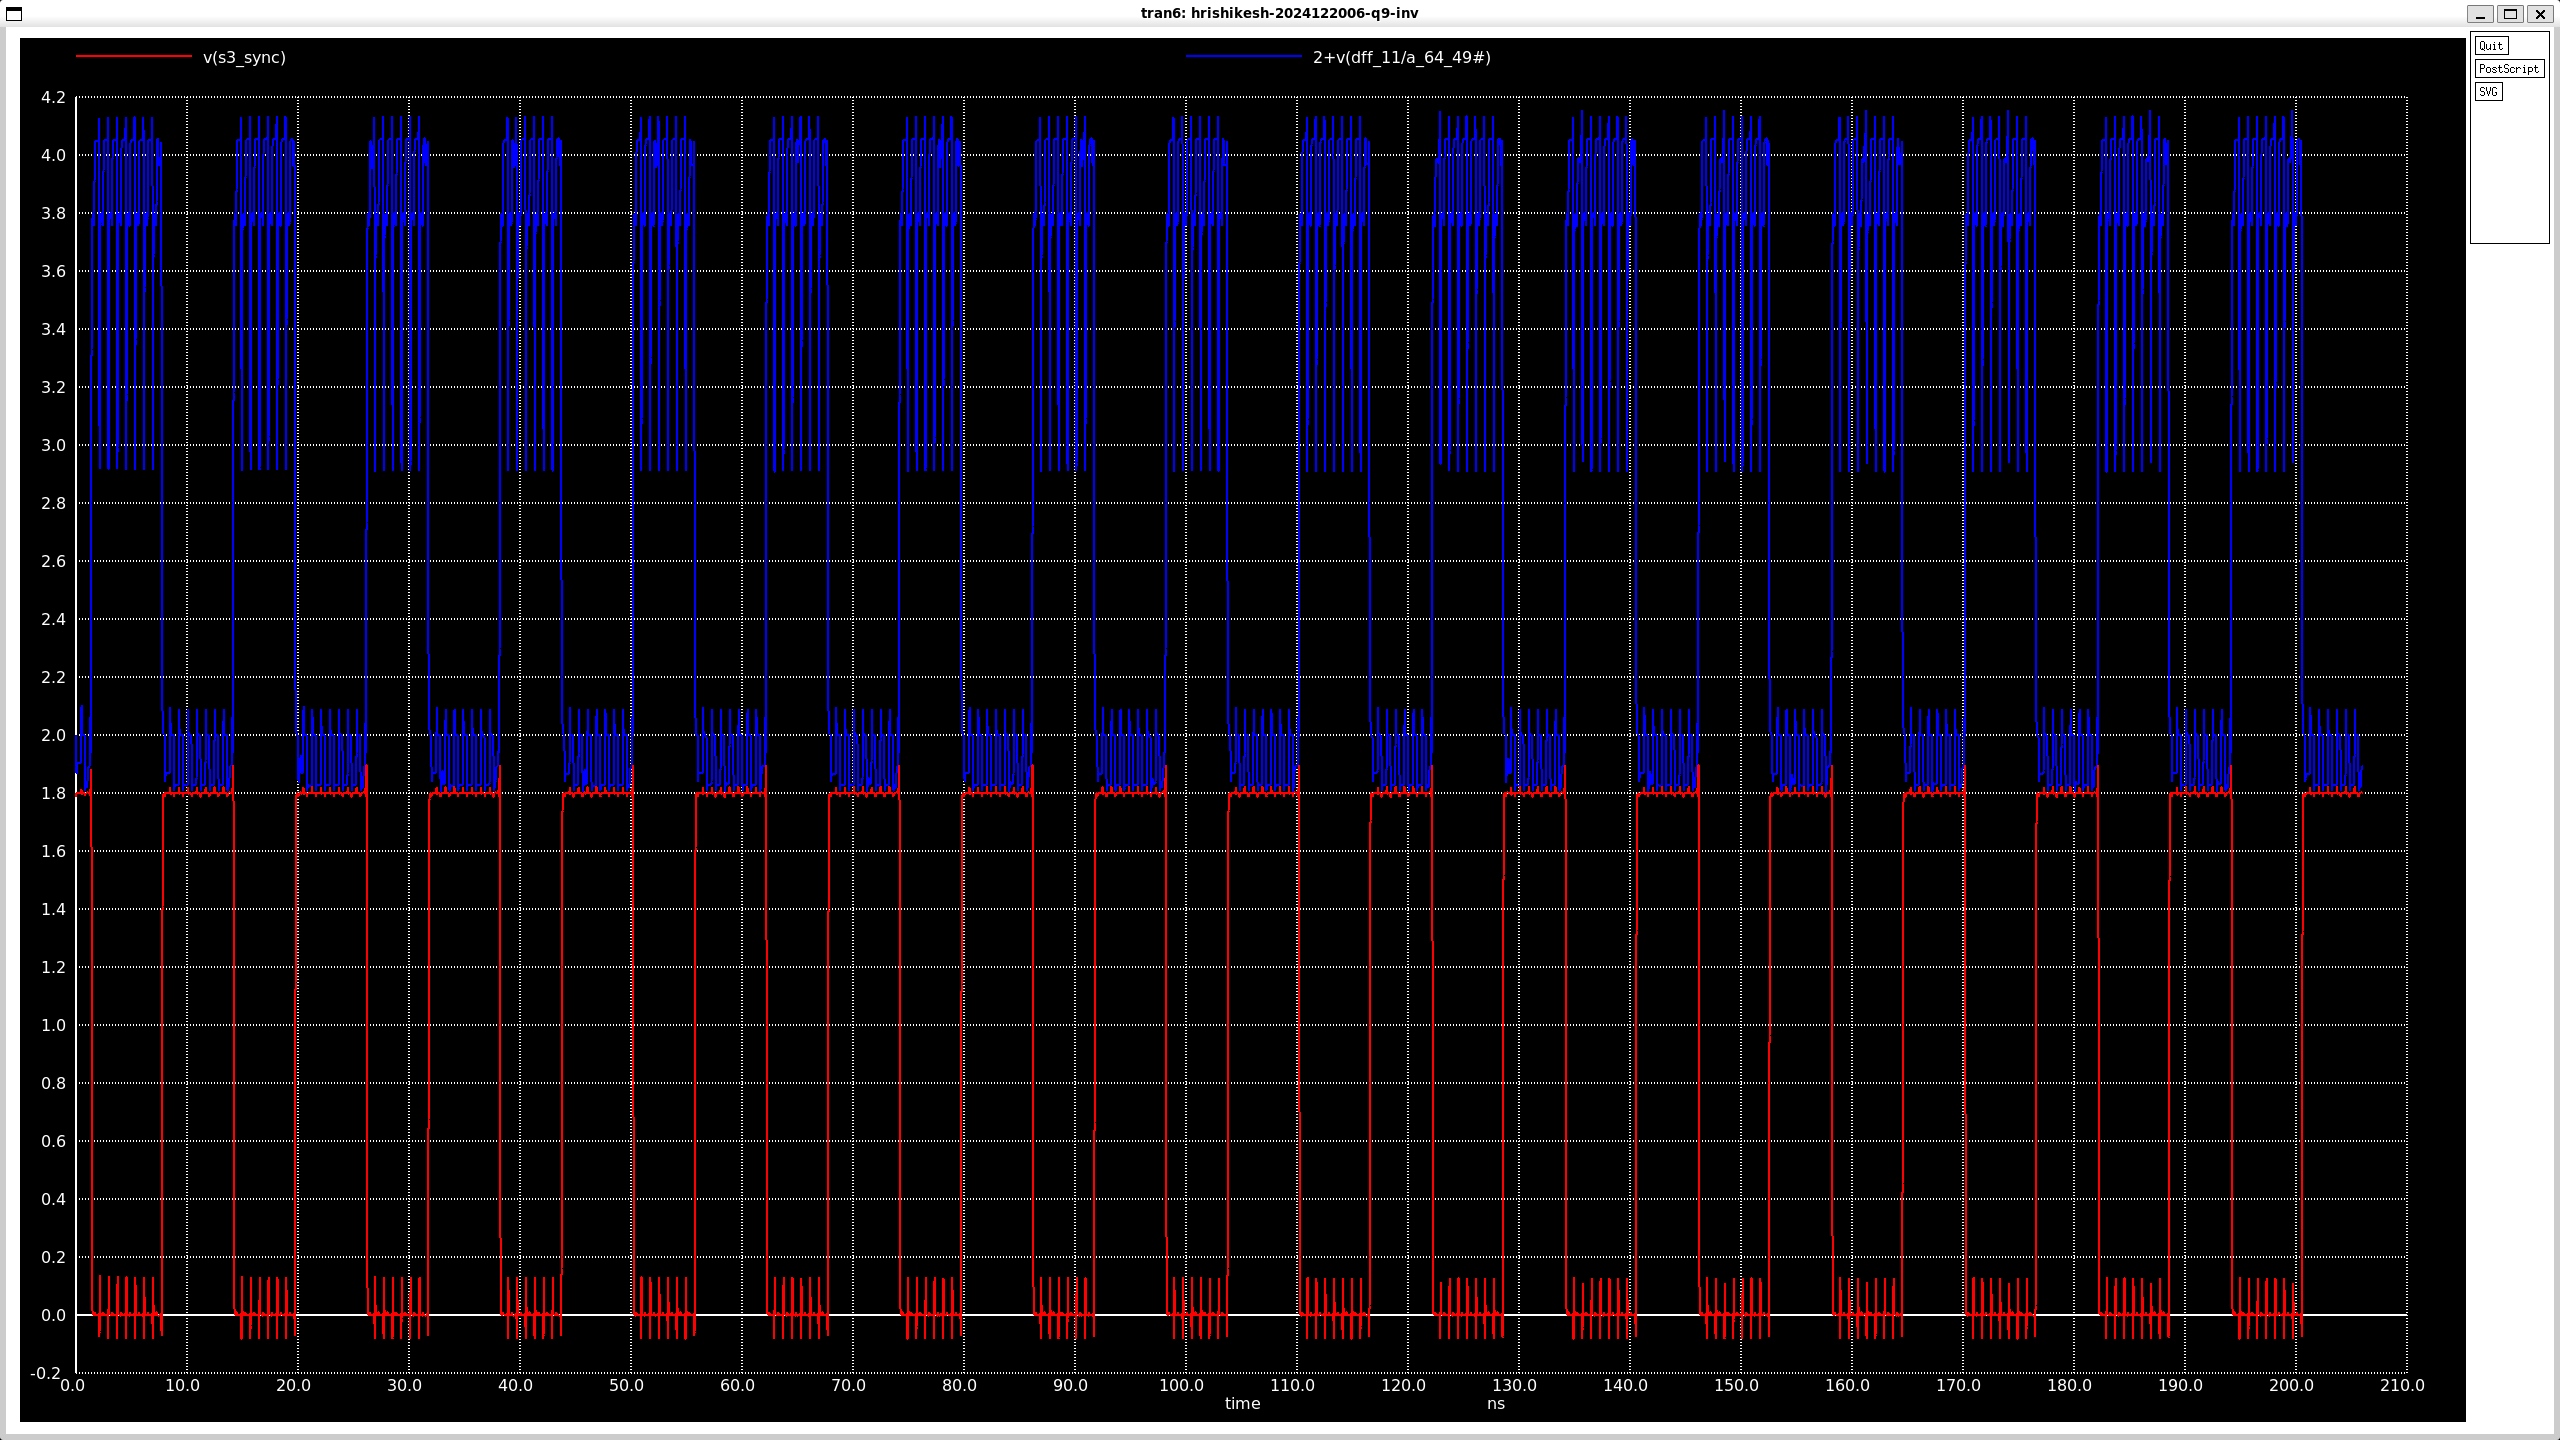
\includegraphics[width=1\linewidth]{final_inv.png}
    \caption{Inverter}
    \label{fig:enter-label}
\end{figure}
\begin{figure}[H]
    \centering
    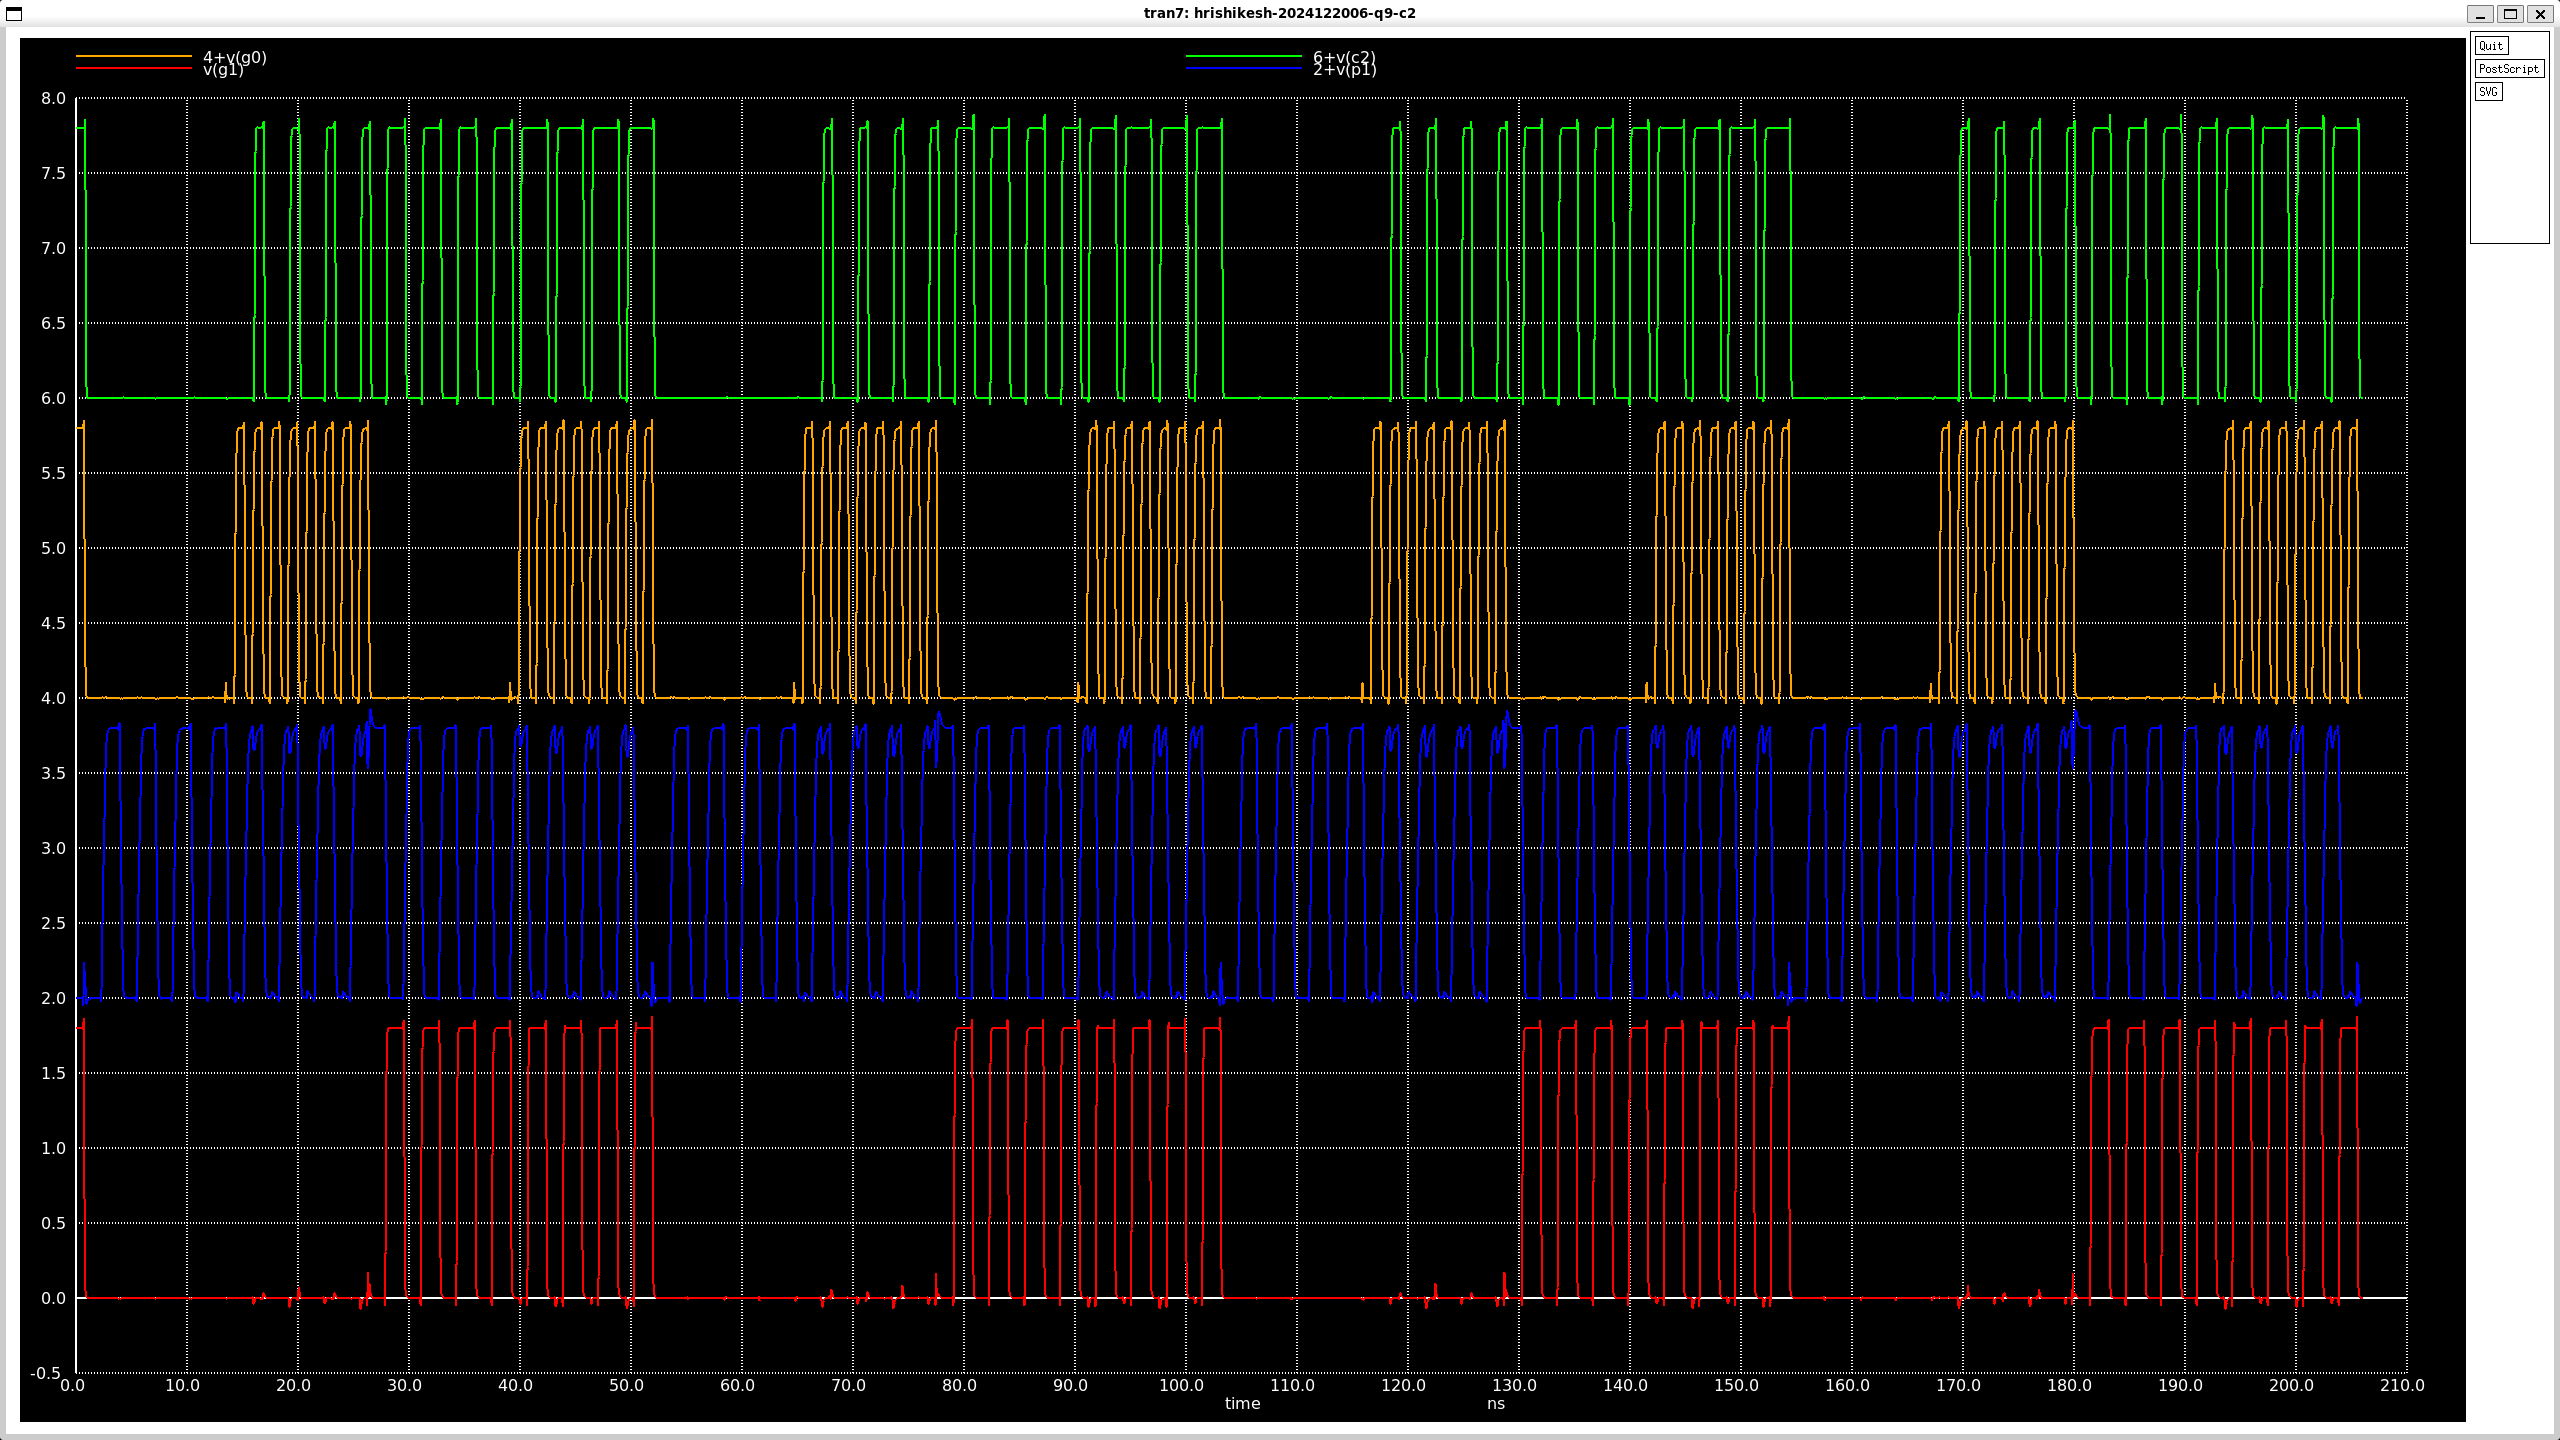
\includegraphics[width=1\linewidth]{final_c2.png}
    \caption{C2 Logic}
    \label{fig:enter-label}
\end{figure}
\begin{figure}[H]
    \centering
    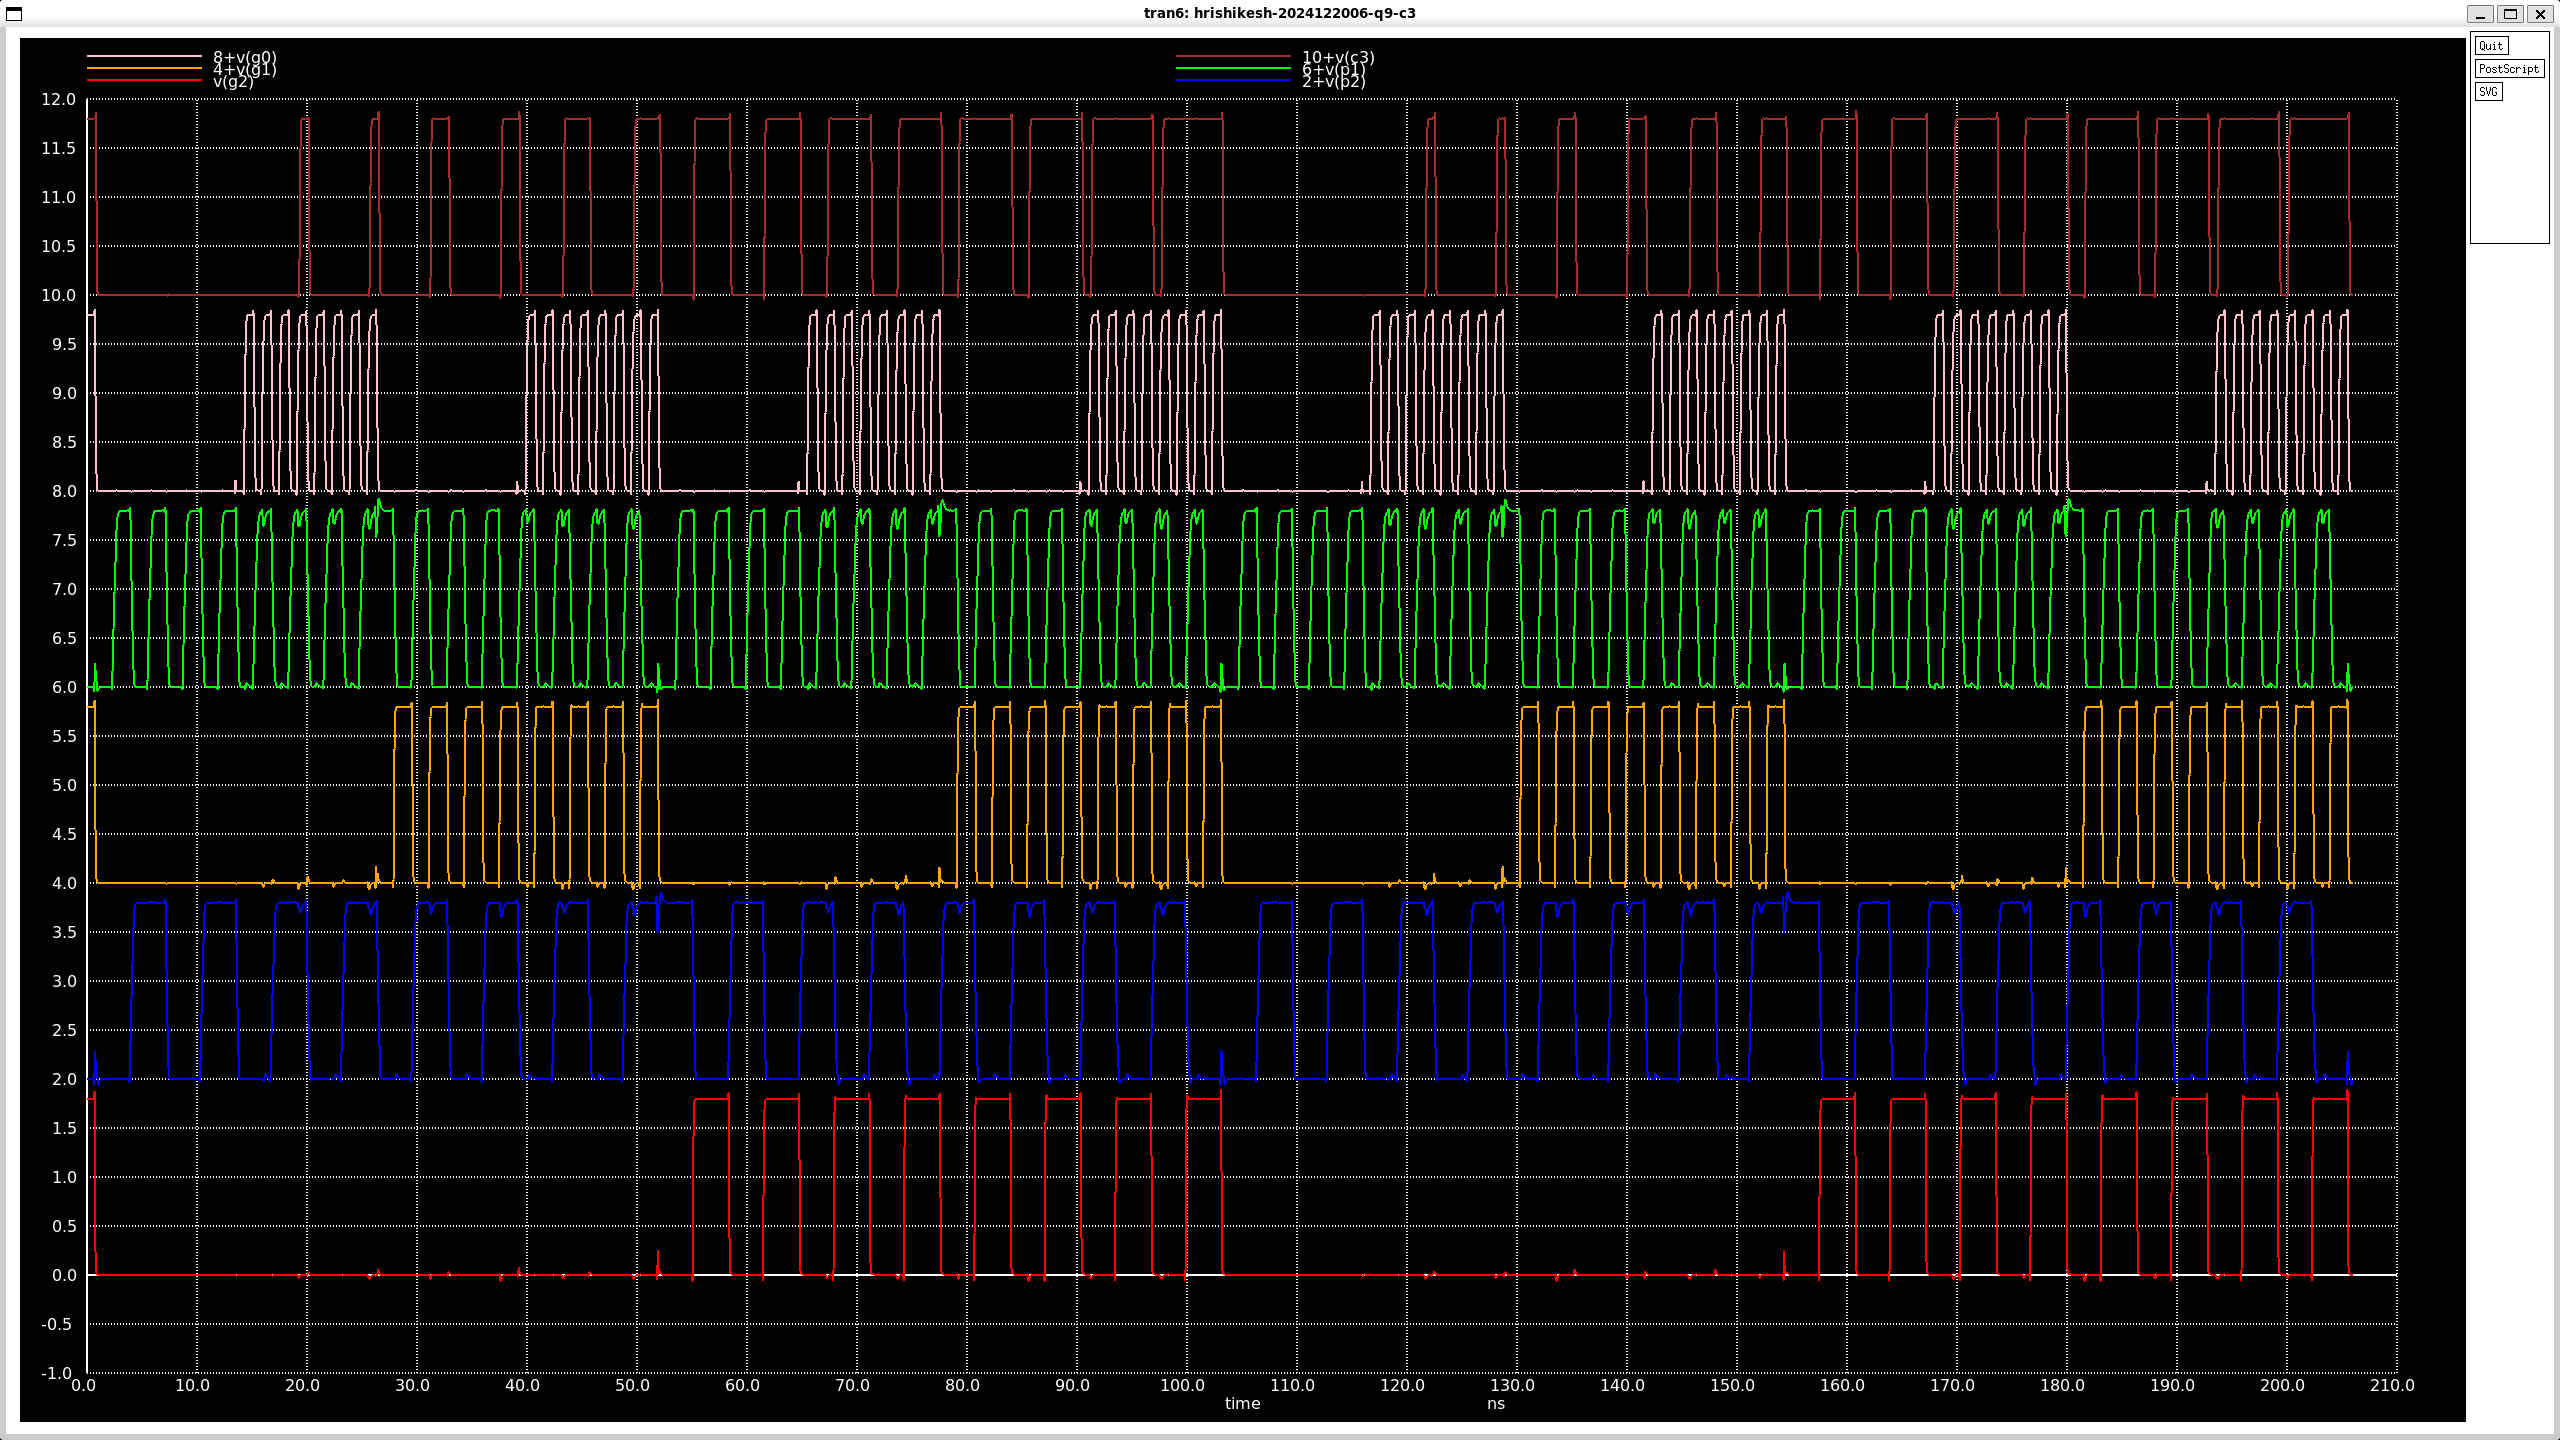
\includegraphics[width=1\linewidth]{final_c3.png}
    \caption{C3 Logic}
    \label{fig:enter-label}
\end{figure}
\begin{figure}[H]
    \centering
    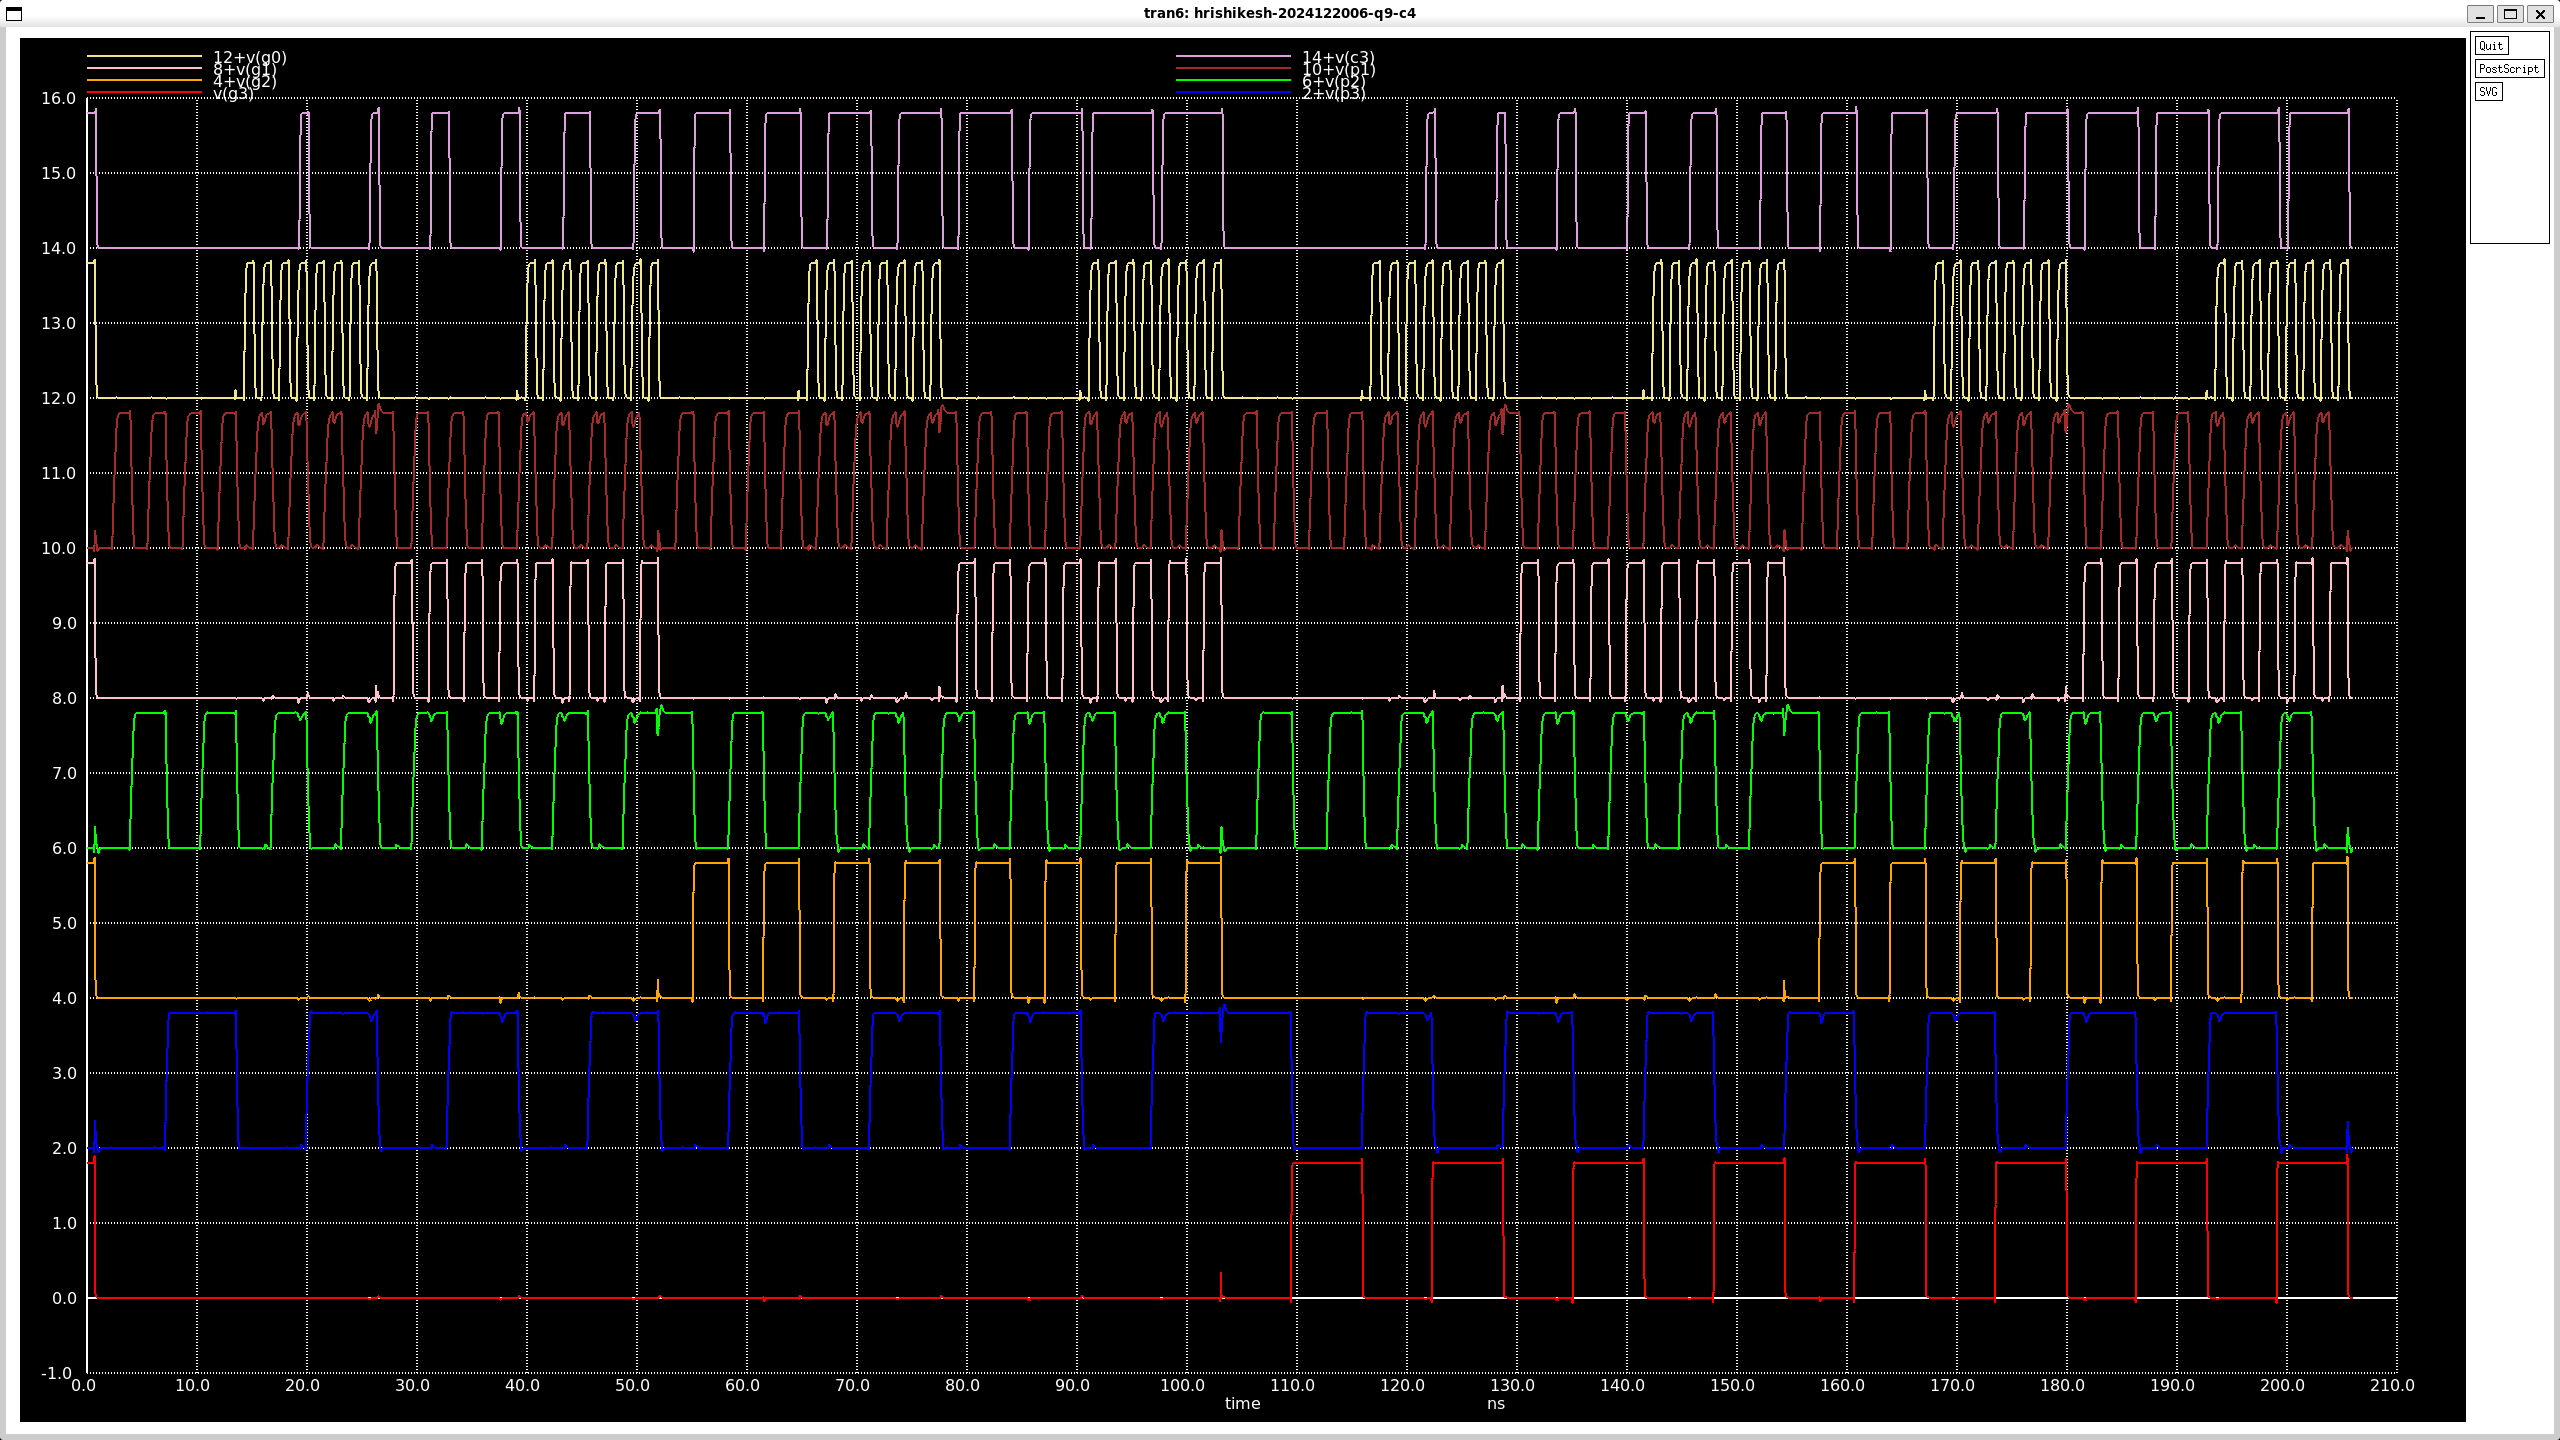
\includegraphics[width=1\linewidth]{final_c4.png}
    \caption{C4 Logic}
    \label{fig:enter-label}
\end{figure}
Post Final Layout Characteristics are compared with schematic and tabulated in TABLE III and IV.
\begin{table*}[ht]
\centering
\caption{Comparison of Pre-Layout and Post-Layout Characteristics for Modules}
\begin{tabular}{|m{4cm}|m{3cm}|m{3cm}|}
\hline
\multirow{2}{*}{\textbf{Module}} & \multicolumn{1}{c|}{\textbf{Pre-Layout Delay (s)}} & \multicolumn{1}{c|}{\textbf{Post-Layout Delay (s)}} \\ 
\hline
Inverter & $5.30549 \times 10^{-11}$ & $5.30549 \times 10^{-11}$ \\ 
\hline
XOR Gate & $1.38618 \times 10^{-10}$ & $2.53084 \times 10^{-10}$ \\ 
\hline
AND Gate & $1.59971 \times 10^{-10}$ & $1.56867 \times 10^{-10}$ \\ 
\hline
$C_2$ Logic & $2.86838 \times 10^{-10}$ & $2.98419 \times 10^{-10}$ \\ 
\hline
$C_3$ Logic & $3.89675 \times 10^{-10}$ & $3.70521 \times 10^{-10}$ \\ 
\hline
$C_4$ Logic & $4.97499 \times 10^{-10}$ & $4.47938 \times 10^{-10}$ \\ 
\hline
\end{tabular}
\label{tab:module_comparison}
\end{table*}
% DFF Comparison Table
\begin{table*}[ht]
\centering
\caption{Comparison of Pre-Layout and Final Post-Layout Characteristics for DFF}
\begin{tabular}{|c|c|c|c|c|c|c|}
\hline
\multirow{2}{*}{\textbf{Transition}} & \multicolumn{3}{c|}{\textbf{Pre-Layout Characteristics}} & \multicolumn{3}{c|}{\textbf{Post-Layout Characteristics}} \\ \cline{2-7}
& \boldmath$t_{\text{setup}}$ & \boldmath$t_{\text{hold}}$ & \boldmath$t_p$ & \boldmath$t_{\text{setup}}$ & \boldmath$t_{\text{hold}}$ & \boldmath$t_p$ \\ \hline
Low to High & 24 ps * & 40 ps * & $8.953852 \times 10^{-11}$ & 24 ps * & 40 ps * & $1.197837 \times 10^{-10}$ \\ \hline
High to Low & 50 ps & 30 ps & $1.466006 \times 10^{-10}$ & 30 ps & 30 ps & $1.737175 \times 10^{-10}$ \\ \hline
Final & 50 ps & 30 ps & $1.18070 \times 10^{-10}$ & 30 ps & 30 ps & $1.46751 \times 10^{-10}$ \\ \hline
\end{tabular}
\label{tab:dff_comparison}
\end{table*}
\newline
\textbf{Worst Case Delay: } Worst case delay if obtained on the critical path. Inputs to all other paths are kept constant. Inputs are chosen such that by only toggling the critical path input, the critical path output changes. The rise and fall time propagation delays are noted.\newline
In this case, a0 to s3 is the critical path which remains the same as last case.
\begin{figure}[H]
    \centering
    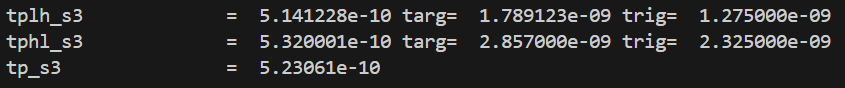
\includegraphics[width=1\linewidth]{q9_tp.png}
    \caption{CLA Propagation Delay}
    \label{fig:enter-label}
\end{figure}
The case with maximum $t_p$ (lh or hl) was chosen to calculate Maximum Clock Frequency.
\[
    t_{CLK} \geq t_p + t_{setup} + t_{pcq} = 532 + 30 + 174 = 736 ps
\]
But certain flaws were noticed at exact time period of 736 ps, therefore for reliable operation a time period of 800 ps was chosen. This equates to 1.25 GHZ of max clock frequency.

\textbf{Circuit Specifications}\newline
RMS Current = 2.996 mA\newline
RMS Power = 5.393 mW\newline
Considering delay offered by CLA combinational circuit only
Power Delay Product = 3.97e-12 Ws


\section{Verilog Implementation and Verification with Oscilloscope}
\begin{figure*}[ht]
    \centering
    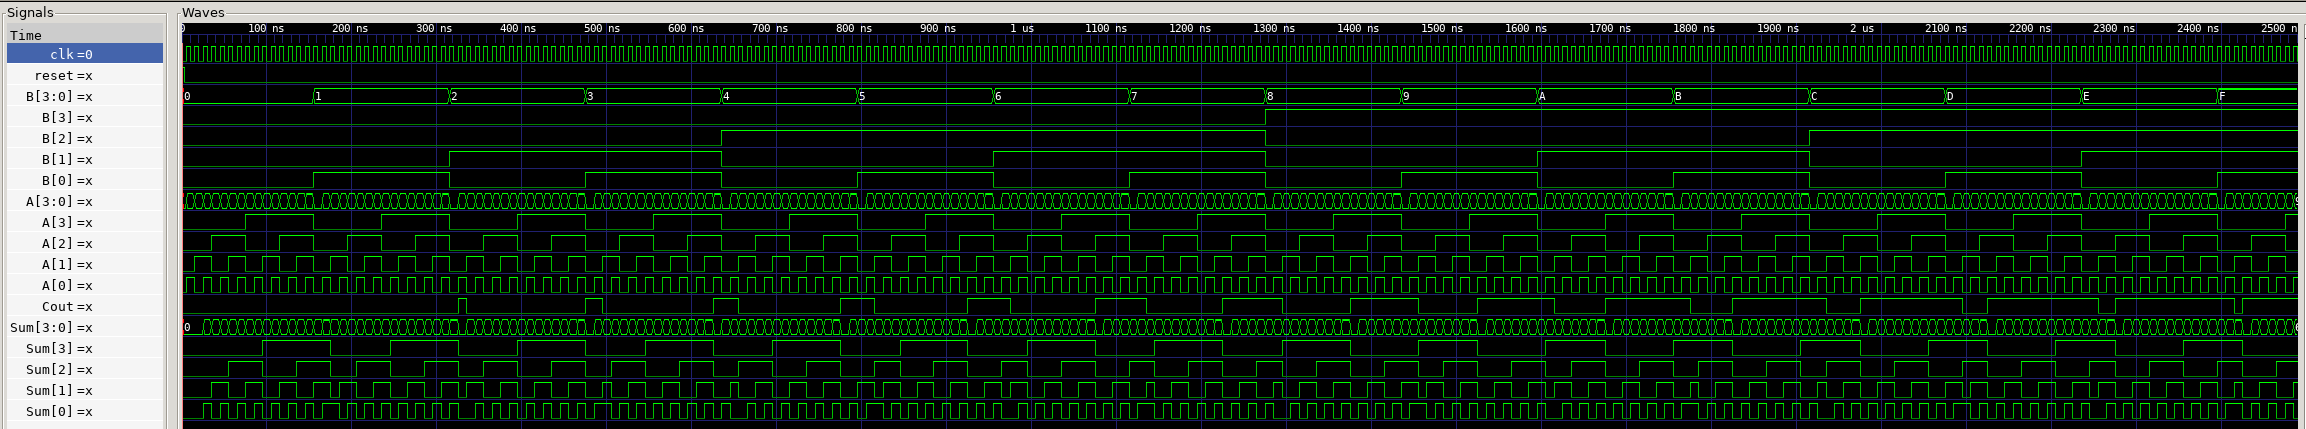
\includegraphics[width=1\linewidth]{gtkwave.png}
    \caption{GTKWave Verification}
    \label{fig:enter-label}
\end{figure*}
The clk was internally divided and provided as inputs to produce all possible 256 combinations of sum. This was viewed on a Oscilloscope (Logic Analyzer -- Digital Probe). The channel if viewed from top to bottom are in order of outputs: C4 S3 S2 S1 S0.
\begin{figure*}[ht]
    \centering
    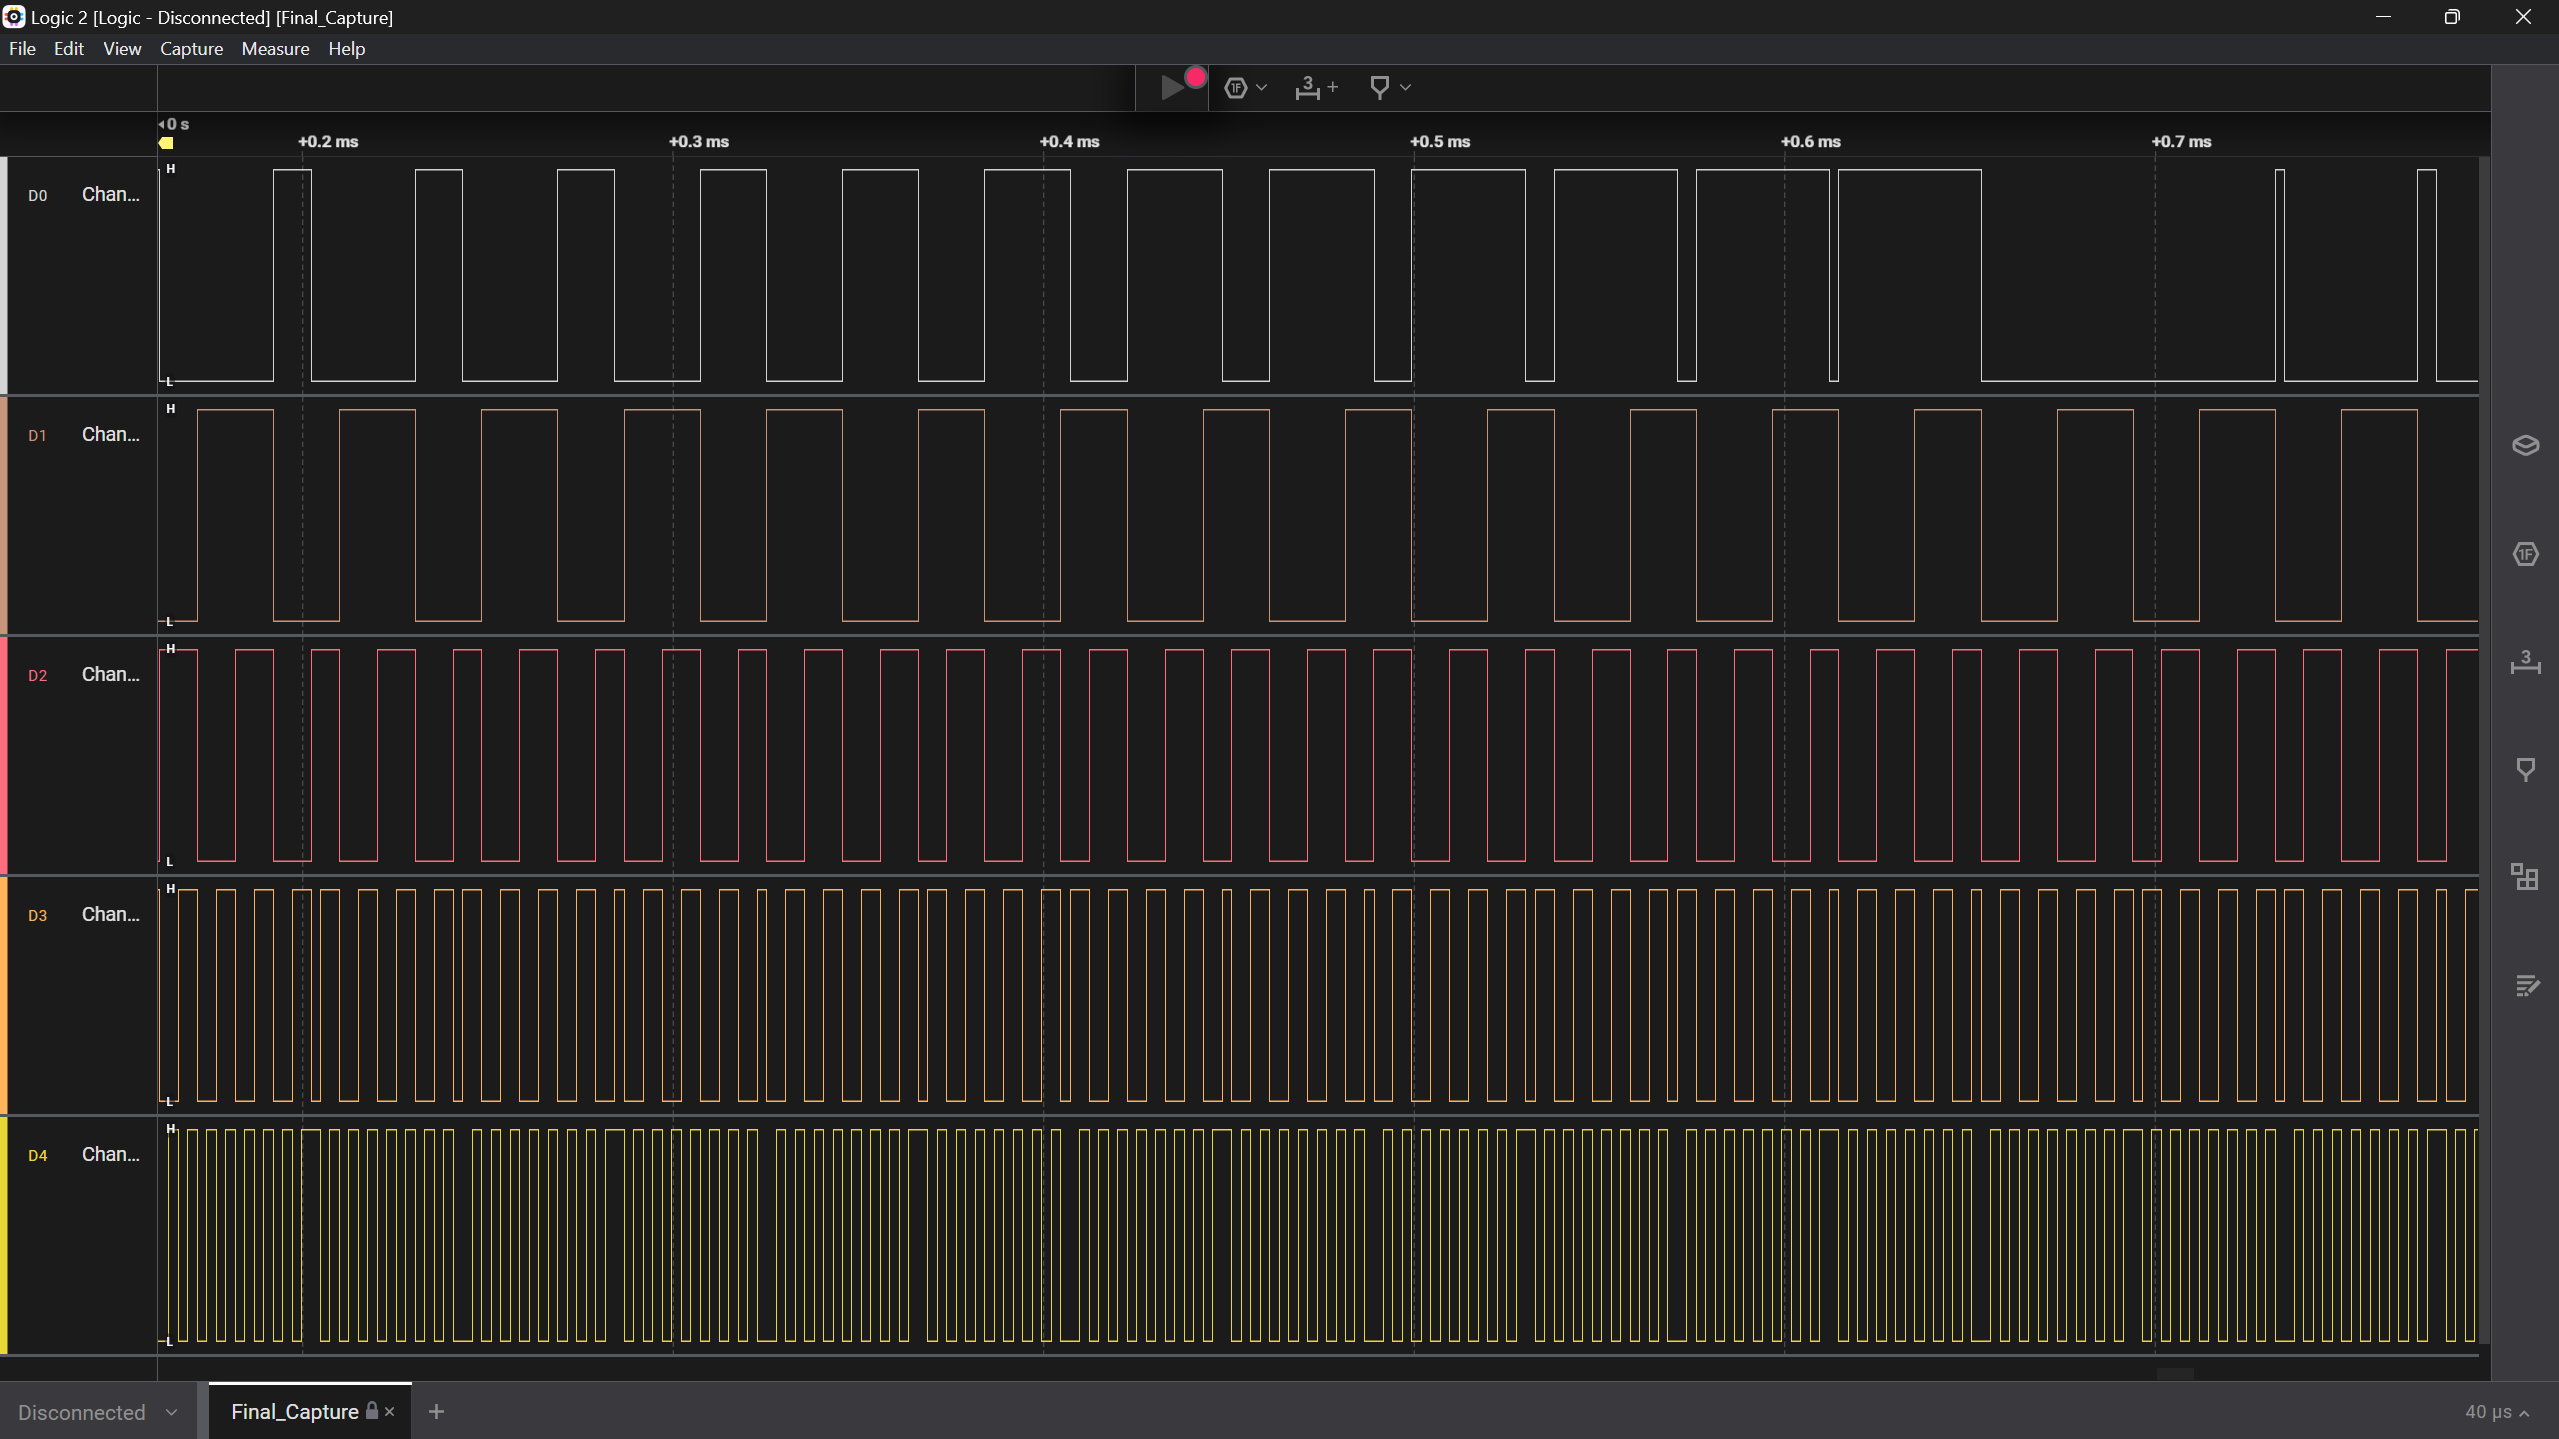
\includegraphics[width=1\linewidth]{logic_analyzer.png}
    \caption{Oscilloscope Capture}
    \label{fig:enter-label}
\end{figure*}
Test Setup:
\begin{figure*}[ht]
    \centering
    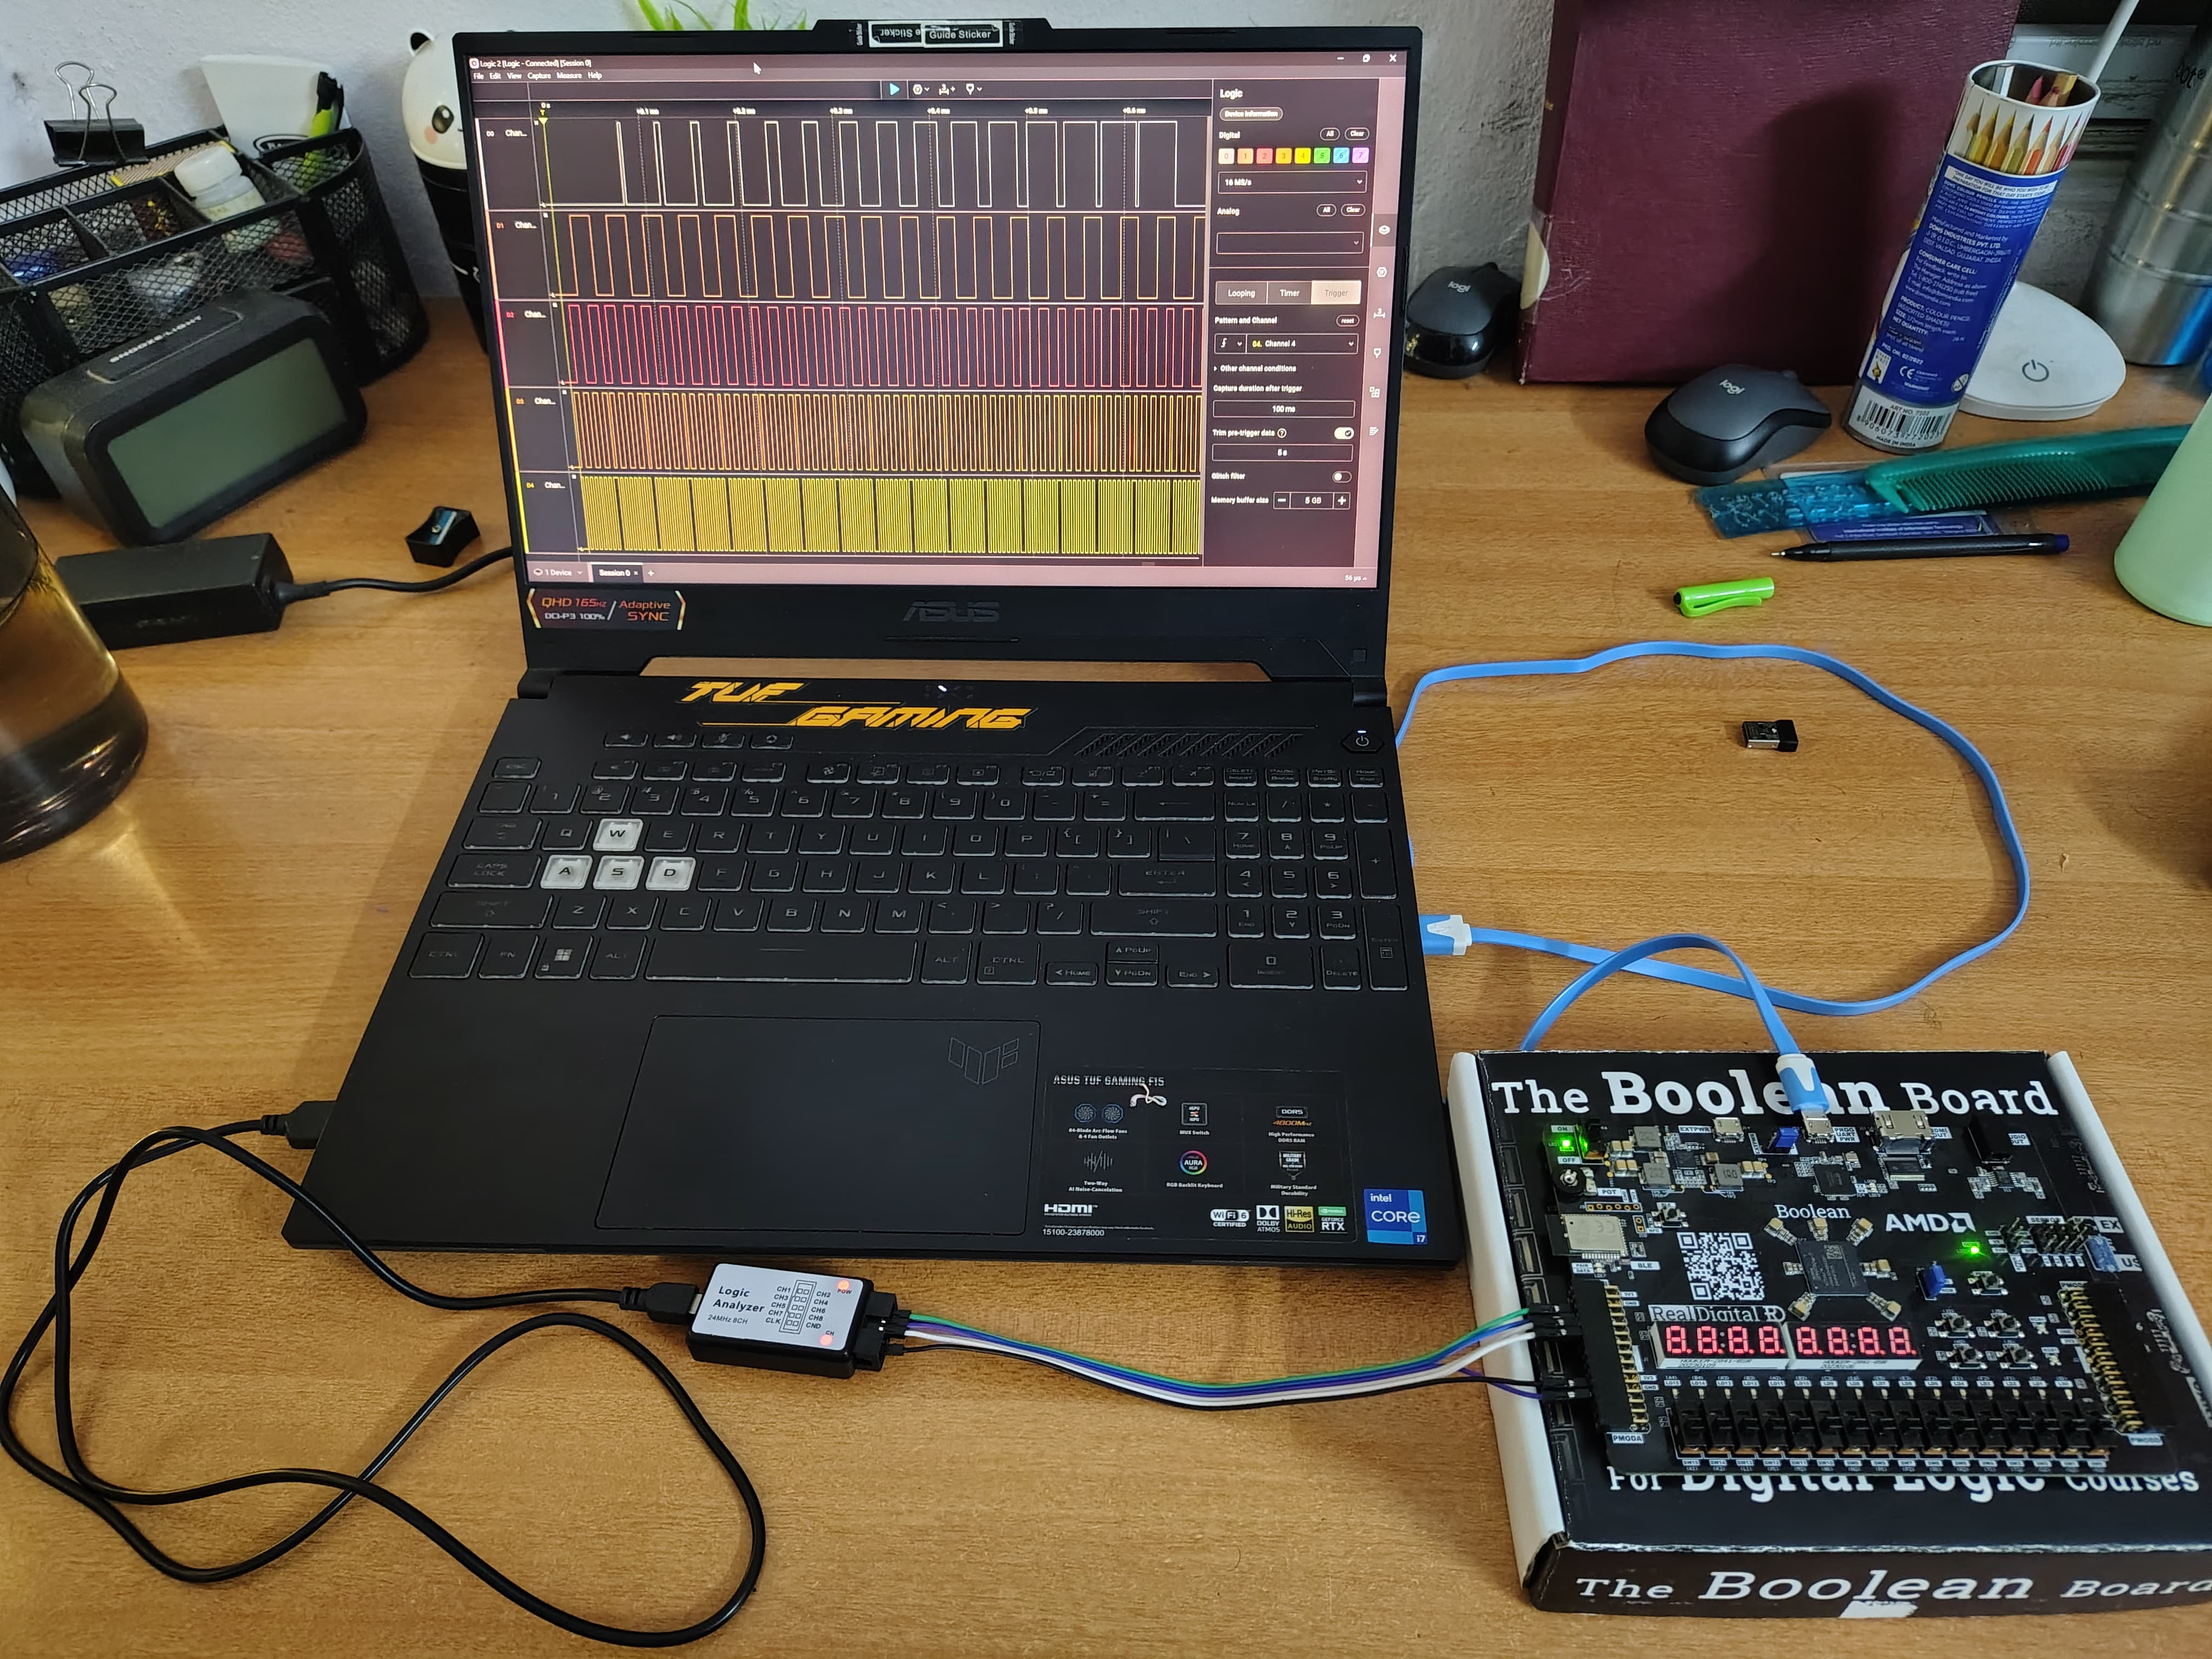
\includegraphics[width=1\linewidth]{Oscilloscope_TestSetup.jpg}
    \caption{Test Setup}
    \label{fig:enter-label}
\end{figure*}

\section{References}
\begin{itemize}
    \item Md. Ashik Zafar Dipto, Elias Ahammad Sojib, Afran Sorwar, Md. Mostak Tahmid Rangon," Performance Improvement in Conventional 4-bit Static CMOS Carry Look-Ahead Adder by Modifying Carry-Generate and Propagate Terms", 11th ICCCNT 2020, July 1-3, 2020-IIT-Kharagpur.
    \item Behzad Razavi, "A Ciruit for All Seasons - TSPC Logic", IEEE SOLID-STATE CIRCUITS MAGAZINE, FALL 2016.
    \item CMOS VLSI Design (fourth edition) by Weste and Harris.
\end{itemize}



\end{document}
